\documentclass{tropLaClasse}

%----------- Report Information ---------

% The type of report
\typestage{M1 Internship Report}

% The location of the internship
\institut{Institute of Science Tokyo}
\laboratoire{Nakashima Laboratory}

% The REAL title of your internship
\titre{Study on Motion Control for the Humanoid Swimming Robot SWUMANOID}

% Your information
\eleve{Clément MESPOUILLES}
\mention{Master of Engineering Sciences -- Sorbonne University}
\filiere{ROBOT Track}
\master{Student ID: 21207226}
\trigrammemention{CMI Mechanics}

% Dates
\dates{01/06/2026 -- 31/08/2026}

% Supervisors and year
\annee{2025/2026}
\tuteurentreprise{
    Motomu NAKASHIMA\\
    Hiroki YANADORI\\
    Daito NAGATA

}

%----------- Initialization -------------------
\logoentreprise{logos/logo_tokyo.png}

\begin{document}

\fairemarges
\fairepagedegarde

% ==========================================
%                 ABSTRACT
% ==========================================
\clearpage
\pagestyle{empty} % No page number for the abstract
\section*{Abstract}
\textit{This report presents the work conducted during my M1 internship at the Nakashima Laboratory, focusing on the SWUMANOID humanoid swimming robot project. The objective of my internship was to improve and modernize the command and control system of the robot. To achieve this, I designed and assembled a new main control board and developed a web interface. This new architecture allows the operator to communicate directly with the robot and provides real-time access to all critical telemetry and status information during pool experiments. Successfully implementing these upgrades required including the seamless integration of motion files, the mathematical interpolation of joint trajectories for smooth swimming, the optimization of the communication baud rate, and the extraction of spatial orientation angles using IMU data. Ultimately, these contributions have established a reliable and responsive experimental platform for future hydrodynamic research.
}

% ==========================================
%             TABLE OF CONTENTS
% ==========================================
\clearpage
\setcounter{page}{1}
\pagestyle{plain} % Resume page numbering
\tabledematieres  % Command already present in your .cls file!

% ==========================================
%             BODY OF THE REPORT
% ==========================================
\section{Introduction}

\subsection{The Nakashima Laboratory}

The Nakashima Laboratory, led by Professor Motomu Nakashima, belongs to the \textbf{Institute of Science Tokyo}. This university represents the merger of the \textit{Tokyo Institute of Technology} (Tokyo Tech) and the \textit{Tokyo Medical and Dental University} (TMDU) \cite{isct2024merger}. The result is an institution built around "convergence science", bringing together engineering, advanced technology, biology and medicine \cite{isct2024merger}. The Nakashima Laboratory sits right at that crossroads, where fundamental mechanics meets human physiology.

Its focus is biomechanics and sports engineering. The main goal is to use robotics and computation to better understand, simulate and reproduce the complex dynamics of the human body \cite{nakashimalab_website}. Working from mathematical models and detailed simulations, such as the SWUM model, which couples rigid-body dynamics with unsteady fluid forces \cite{nakashima2007swum}, the team analyzes and optimizes human motion in different environments. The work spans several scales, from the macroscopic study of fluid forces to a fine musculo-skeletal analysis of physical effort, as shown in the figure \ref{fig:simulations_labo}.

\begin{figure}[H]
    \centering
    \begin{subfigure}[b]{0.42\textwidth}
        \centering
        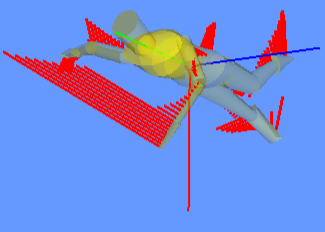
\includegraphics[width=\textwidth]{Introduction/Nakashima_site_1.png}
        \caption{SWUM model with fluid force vectors.}
    \end{subfigure}
    \hfill
    \begin{subfigure}[b]{0.53\textwidth}
        \centering
        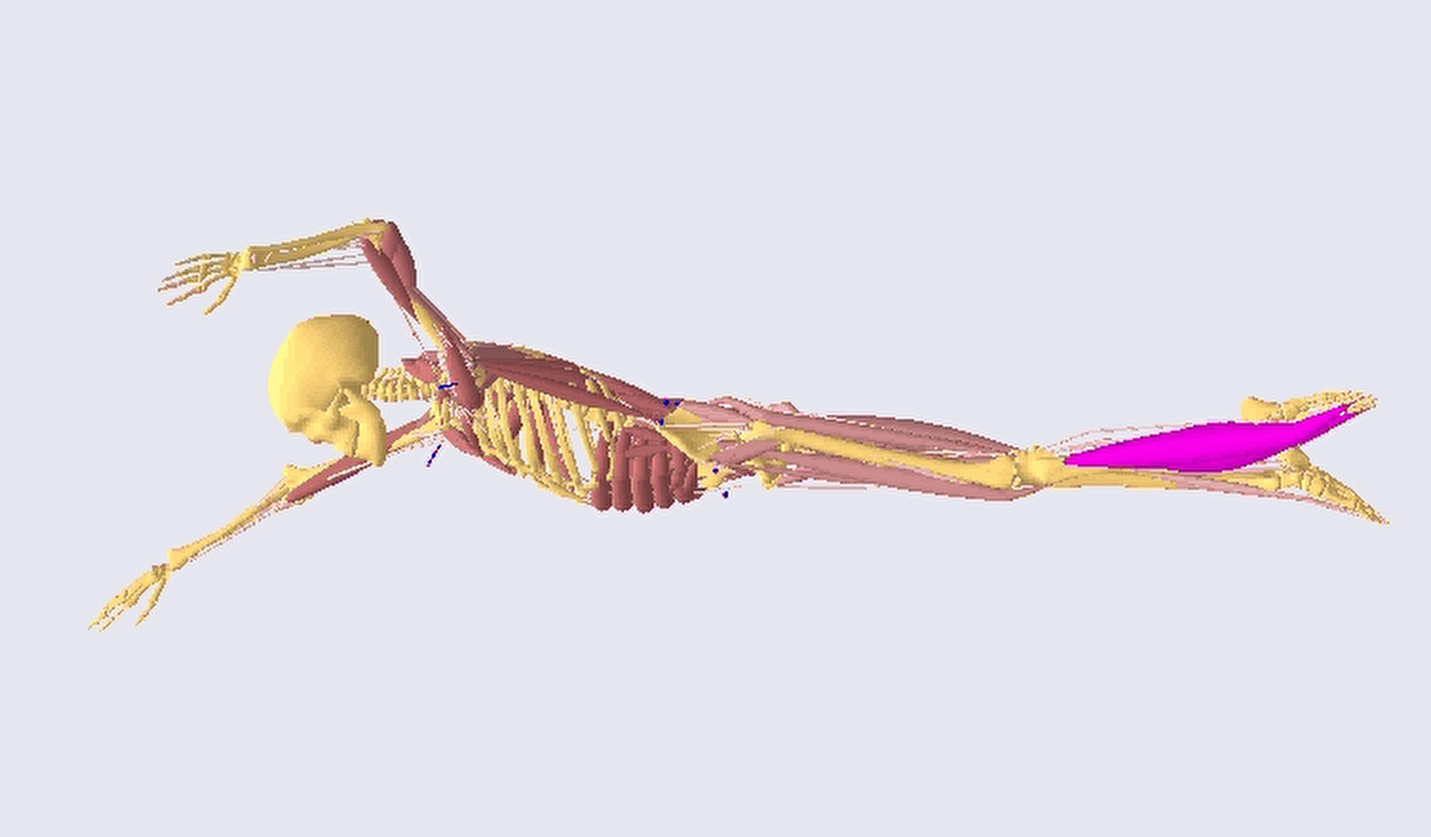
\includegraphics[width=\textwidth]{Introduction/Nakashima_site_5.png}
        \caption{Musculo-skeletal model of swimming.}
    \end{subfigure}
    \caption{Simulations used in the laboratory to study body dynamics.}
    \label{fig:simulations_labo}
\end{figure}

The research is not limited to water, in fact it reaches into many everyday and athletic biomechanical problems for example the body dynamics during wheelchair tennis matches, the study of mass distribution and body management during sleep, and the modeling of effort in redundant human tasks.

\begin{figure}[H]
    \centering
    \begin{subfigure}[b]{0.32\textwidth}
        \centering
        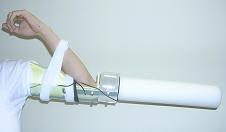
\includegraphics[width=\textwidth]{Introduction/Nakashima_site_6.png}
        \caption{Biomechanical measurement device.}
    \end{subfigure}
    \hfill
    \begin{subfigure}[b]{0.32\textwidth}
        \centering
        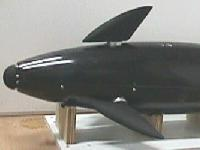
\includegraphics[width=\textwidth]{Introduction/Nakashima_site_4.png}
        \caption{Biomimetic aquatic robot.}
    \end{subfigure}
    \hfill
    \begin{subfigure}[b]{0.32\textwidth}
        \centering
        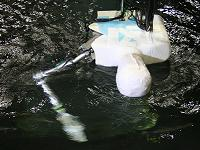
\includegraphics[width=\textwidth]{Introduction/Nakashima_site_2.png}
        \caption{Robotic prototype in a pool.}
    \end{subfigure}
    \caption{Physical experimental platforms developed by the laboratory \cite{nakashimalab_website}.}
    \label{fig:prototypes_labo}
\end{figure}

To test these models in the real world, the lab designs and runs a wide range of experimental devices, shown in the figure \ref{fig:prototypes_labo}. They range from wearable measurement systems for the upper limbs to biomimetic aquatic robots, and up to a full swimming humanoid robot, the SWUMANOID. This robot grew out of years of \textit{Bio-Robotics} research, and it is the project I joined.


\subsection{The SWUMANOID Project}

When I arrived at the lab, I joined the SWUMANOID project. Its purpose is to get around the limits of swimming experiments run on real humans. In fact, measuring unsteady fluid forces on an actual swimmer is hard because the subject gets tired, sensors are difficult to mount reliably underwater, and no human can repeat a stroke with perfect consistency \cite{chung2014swimming} \cite{nakashima2016realization}.

To sidestep all of this, the lab built a complete swimming humanoid robot that acts as a stand-in experimental platform \cite{chung2014swimming} \cite{nakashima2016realization}. The base model was designed by reproducing the body geometry of an elite swimmer captured in a 3D scan \cite{chung2013free} \cite{nakashima2016realization}. Figure \ref{fig:modeles_3d} shows this biomimetic approach, comparing the 3D mesh of a real swimmer with the CAD shell adapted for the SWUMANOID.

\begin{figure}[H]
    \centering
    \begin{subfigure}[b]{0.45\textwidth}
        \centering
        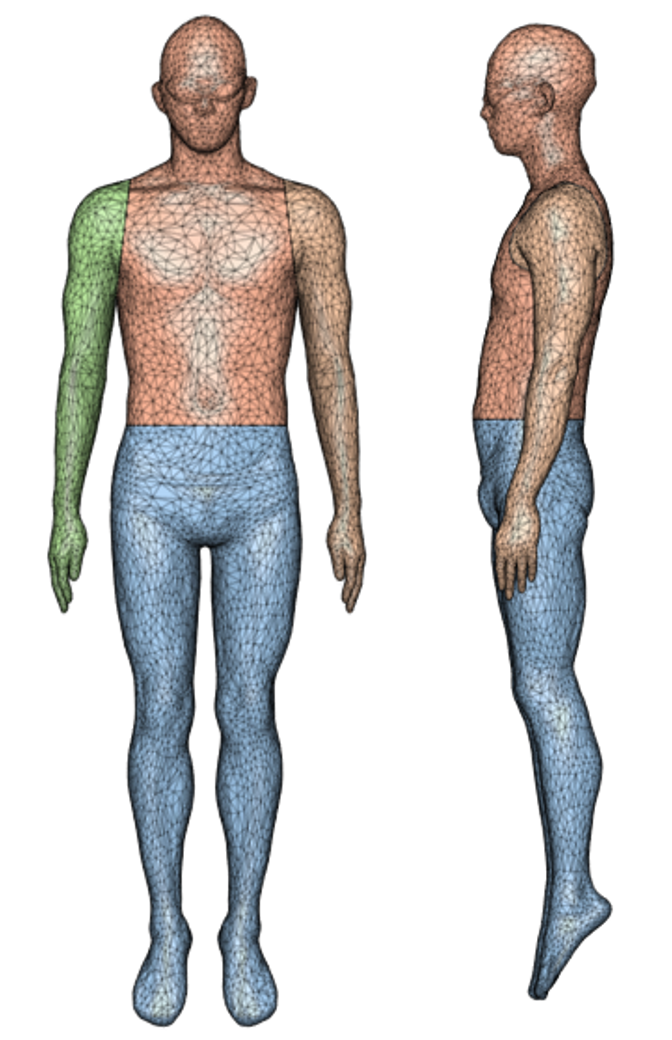
\includegraphics[height=9cm]{Introduction/Model_3D_real_swimmer.png}
        \caption{3D scan of the swimmer}
    \end{subfigure}
    \hfill
    \begin{subfigure}[b]{0.45\textwidth}
        \centering
        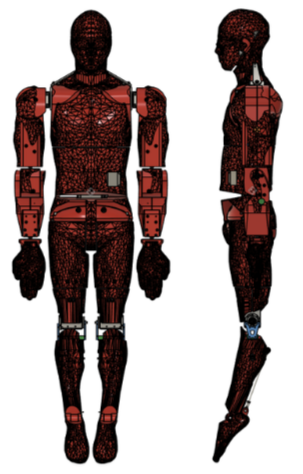
\includegraphics[height=9cm]{Introduction/SWUMANOID_Model_3D.png}
        \caption{3D model adapted for the robot}
    \end{subfigure}
    \caption{Robot geometry derived from the morphology of an elite swimmer.}
    \label{fig:modeles_3d}
\end{figure}

When I joined the project, it was in a transition phase, the previous SWUMANOID, which swam perfectly, had suffered irreversible damage and could no longer be used. A brand-new version, starting from scratch, had been launched only a few months earlier. This full rebuild covered the structure, the skeleton, the 3D printing of every part, new motors, and a rewrite of the motion files. Figure \ref{fig:robot_moteurs} shows this new iteration and the layout of its actuation.

\begin{figure}[H]
    \centering
    \begin{subfigure}[b]{0.45\textwidth}
        \centering
        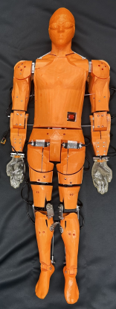
\includegraphics[height=7cm]{Introduction/SWUMANOID_Front_Picture.png}
        \caption{New version of the SWUMANOID}
    \end{subfigure}
    \hfill
    \begin{subfigure}[b]{0.45\textwidth}
        \centering
        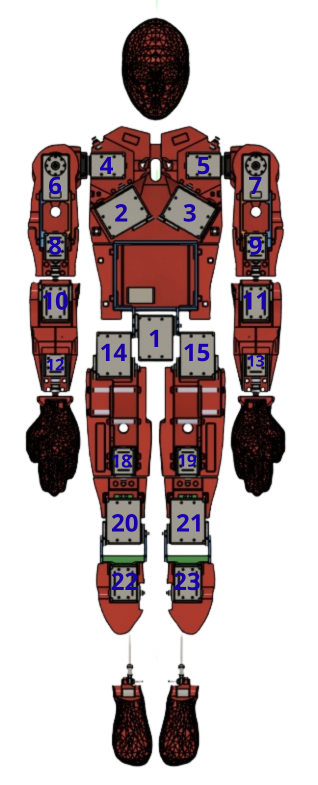
\includegraphics[height=7cm]{Introduction/SWUMANOID_Motors_Ids.png}
        \caption{Motor map and IDs}
    \end{subfigure}
    \caption{Hardware and kinematic overview of the robot.}
    \label{fig:robot_moteurs}
\end{figure}

Building the robot at full human size is not practical, so its scale was reduced. The robot is roughly 50\% of the real swimmer's size \cite{chung2013free} \cite{chung2014swimming}, but the arms of the new version were modeled at 60\% of full scale to make place for the new motors. These motors are more powerful and, above all, IP68-certified, so fully waterproof, which removes any risk of short circuits. The robot weighs about 7.3 kg, close to 10\% of an adult swimmer's weight, in line with the earlier models that weighed between 7.12 kg and 7.4 kg \cite{chung2013free} \cite{nakashima2016realization}.

I joined the SWUMANOID team, a group of three where I work alongside my two supervisors, M. YANADORI and M. NAGATA. When I arrived, the team was finishing tests on new coatings for the 3D-printed parts and before that, the parts filled up with water, which changed the buoyancy and sank the robot. The multi-layer waterproofing process, detailed in the figure \ref{fig:waterproof}, was a decisive step for the integrity of the whole system. We settled on urethane as the coating for the PLA+ printed parts which solved the water infiltration problem, and the robot could finally float the moment I arrived, which had not been the case before.

\begin{figure}[H]
    \centering
    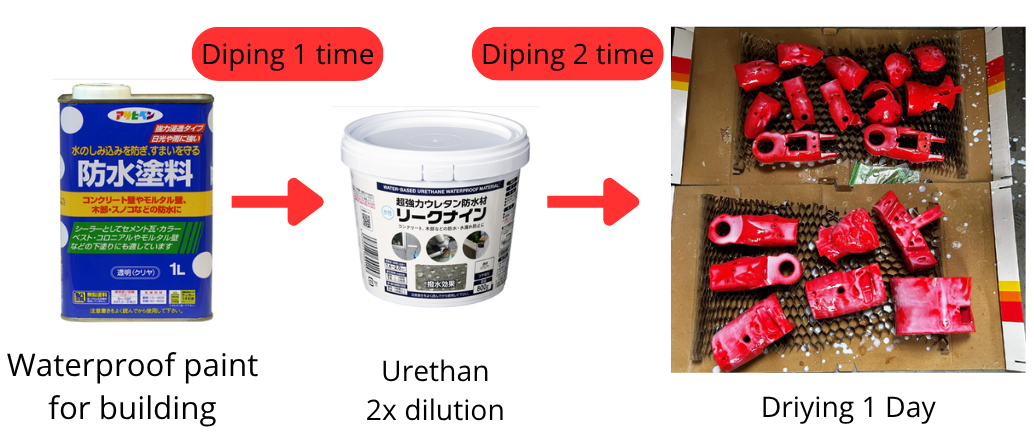
\includegraphics[width=0.85\textwidth]{Introduction/Werproof_method.png}
    \caption{Waterproofing protocol for the PLA+ parts.}
    \label{fig:waterproof}
\end{figure}

Within our trio, the work is clearly split. My two supervisors focus on the theoretical and analytical study of motion, their research relies on the simulation software \textit{SWUMSUIT}. Built to implement the SWUM (Swimming Human Model) simulation model, it computes the absolute motion of the human body in water by solving the equations of motion of a rigid body, and estimates the fluid forces acting on the body from the input geometry and joint motions \cite{swumsuit2005}. The numerical results let us visualize the swimming dynamics and read the vector distribution of the propulsive forces, as the captures in the figure \ref{fig:swumsuit_sim} show.

\begin{figure}[H]
    \centering
    \begin{subfigure}[b]{0.43\textwidth}
        \centering
        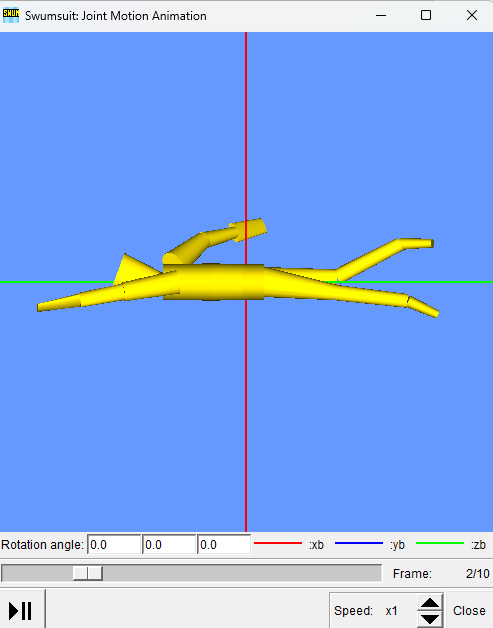
\includegraphics[width=\textwidth]{Introduction/SWAM_simulation.png}
        \caption{Simulation of the joint kinematics}
    \end{subfigure}
    \hfill
    \begin{subfigure}[b]{0.48\textwidth}
        \centering
        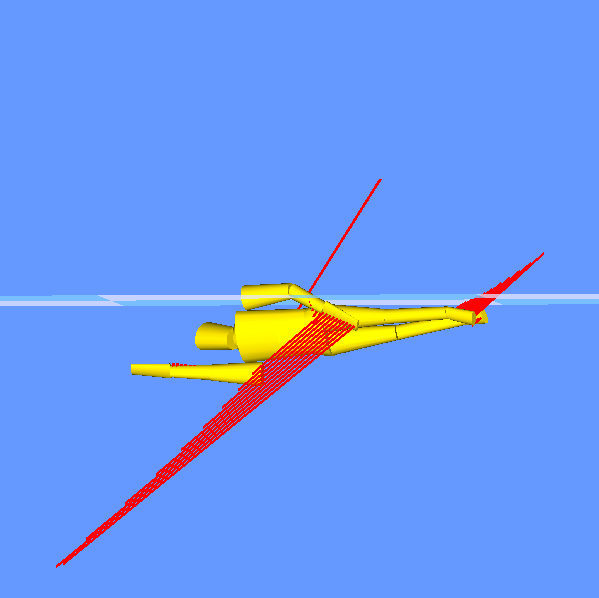
\includegraphics[width=\textwidth]{Introduction/SWAM_simulation_with_force.png}
        \caption{Fluid force vectors (in red)}
    \end{subfigure}
    \caption{Interface and renders of the \textit{SWUMSUIT} simulation software.}
    \label{fig:swumsuit_sim}
\end{figure}

The SWUMSUIT interface can extract swimming data such as swimming speed, propulsive efficiency, and joint torques \cite{swumsuit2005}.
\begin{itemize}
    \item \textbf{NAGATA} works on steering the robot during swimming, with a particular focus on the dynamics of turning strokes.
    \item \textbf{YANADORI} studies the torques generated by the robot's joints while swimming, using the current drawn by the motors.
\end{itemize}

\vspace{0.2cm}

These studies extend the lab's long line of research into how muscular constraints, such as maximum joint torque, shape the speed and propulsive efficiency of human swimmers \cite{nakashima2012optimizing}.

For me, my studies focus on the low-level and hardware control of the SWUMANOID. This split makes us efficient for improving the project? We run roughly two pool experiments a week and during those sessions we test different strokes and iterate on the control parameters, hunting for the settings that lead to a clean, natural swim.

To keep up that pace and make our deployments safe, we have a room dedicated entirely to the project. There, the robot hangs in the air on a bar, which lets us send commands and check the joint motions dry before any immersion. As in the figure \ref{fig:air_test} shows, this suspension rig isolates the actuators so we can debug their mechanical response on its own. This is also where we manage all the hardware and 3D-print new parts to keep improving the robot.

\begin{figure}[H]
    \centering
    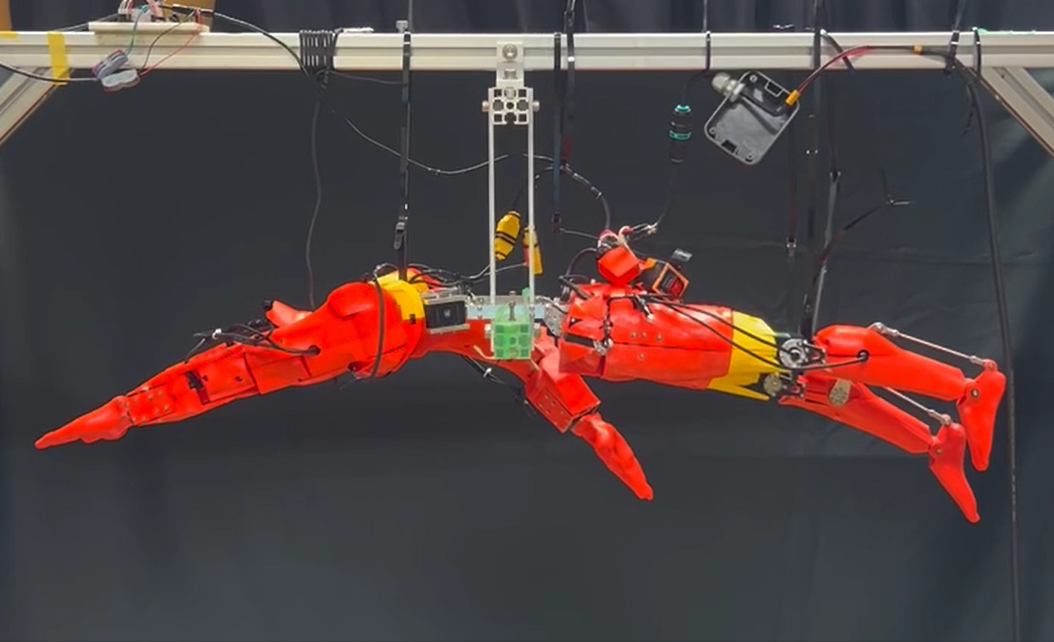
\includegraphics[width=0.6\textwidth]{Introduction/Swumanoid_test_salle_en_l_air.png}
    \caption{Suspended test rig in the laboratory.}
    \label{fig:air_test}
\end{figure}

\subsection{Assigned Missions}

The overall goal of the SWUMANOID project is to provide an experimental platform that reproduces the complex motions of a human swimmer, so we can quantify the unsteady fluid forces generated during swimming \cite{chung2013free, chung2014swimming}. For the measured data to be scientifically usable and comparable to human swimming, the robot has to swim smoothly and without interruption \cite{chung2013free, chung2014swimming}. This is where my work fits with embedded software development, control theory, and experimental validation in the pool. Within the team, I took charge of developing and optimizing the embedded control system, and of running the physical experiments.

\subsubsection*{Control architecture and kinematics}

When I arrived, the previous system was heavily limited because the control frequency was locked at 72 Hz, the Wi-Fi connection was unstable, and other issues that produced mechanical jerks. So my main technical mission was to design a new software and hardware architecture around a more capable microcontroller, the M5Stack AtomS3R. My tasks here were:

\begin{itemize}
    \item \textbf{High-frequency control and hardware interface:} Rethink the communication with the Dynamixel motors' RS-485 bus by studying how the motors react to commands and to design a circuit able to reach a \textit{baudrate} of 3 Mbps. That gives an ultra-fast 200 Hz control loop for all 21 motors, and motion smooth enough not to disturb the fluid dynamics during swimming \cite{chung2014swimming}.
    \item \textbf{Kinematics and trajectory processing:} Implement mathematical smoothing and interpolation to recompute the joint positions at high frequency. The point is to kill the mechanical jolts caused by the acceleration discontinuities of poor interpolation.
    \item \textbf{Spatial configuration and telemetry:} Handle the acquisition from the inertial unit embedded in the robot's head, to configure and track the SWUMANOID's spatial orientation in real time.
    \item \textbf{User Interface (UI) development:} Build a standalone HTML/JavaScript web page to interact with the robot easily. It secures the Wi-Fi connection, converts the motion files directly, and lets the operator tune the control parameters remotely on the fly.
\end{itemize}

\begin{figure}[H]
    \centering
    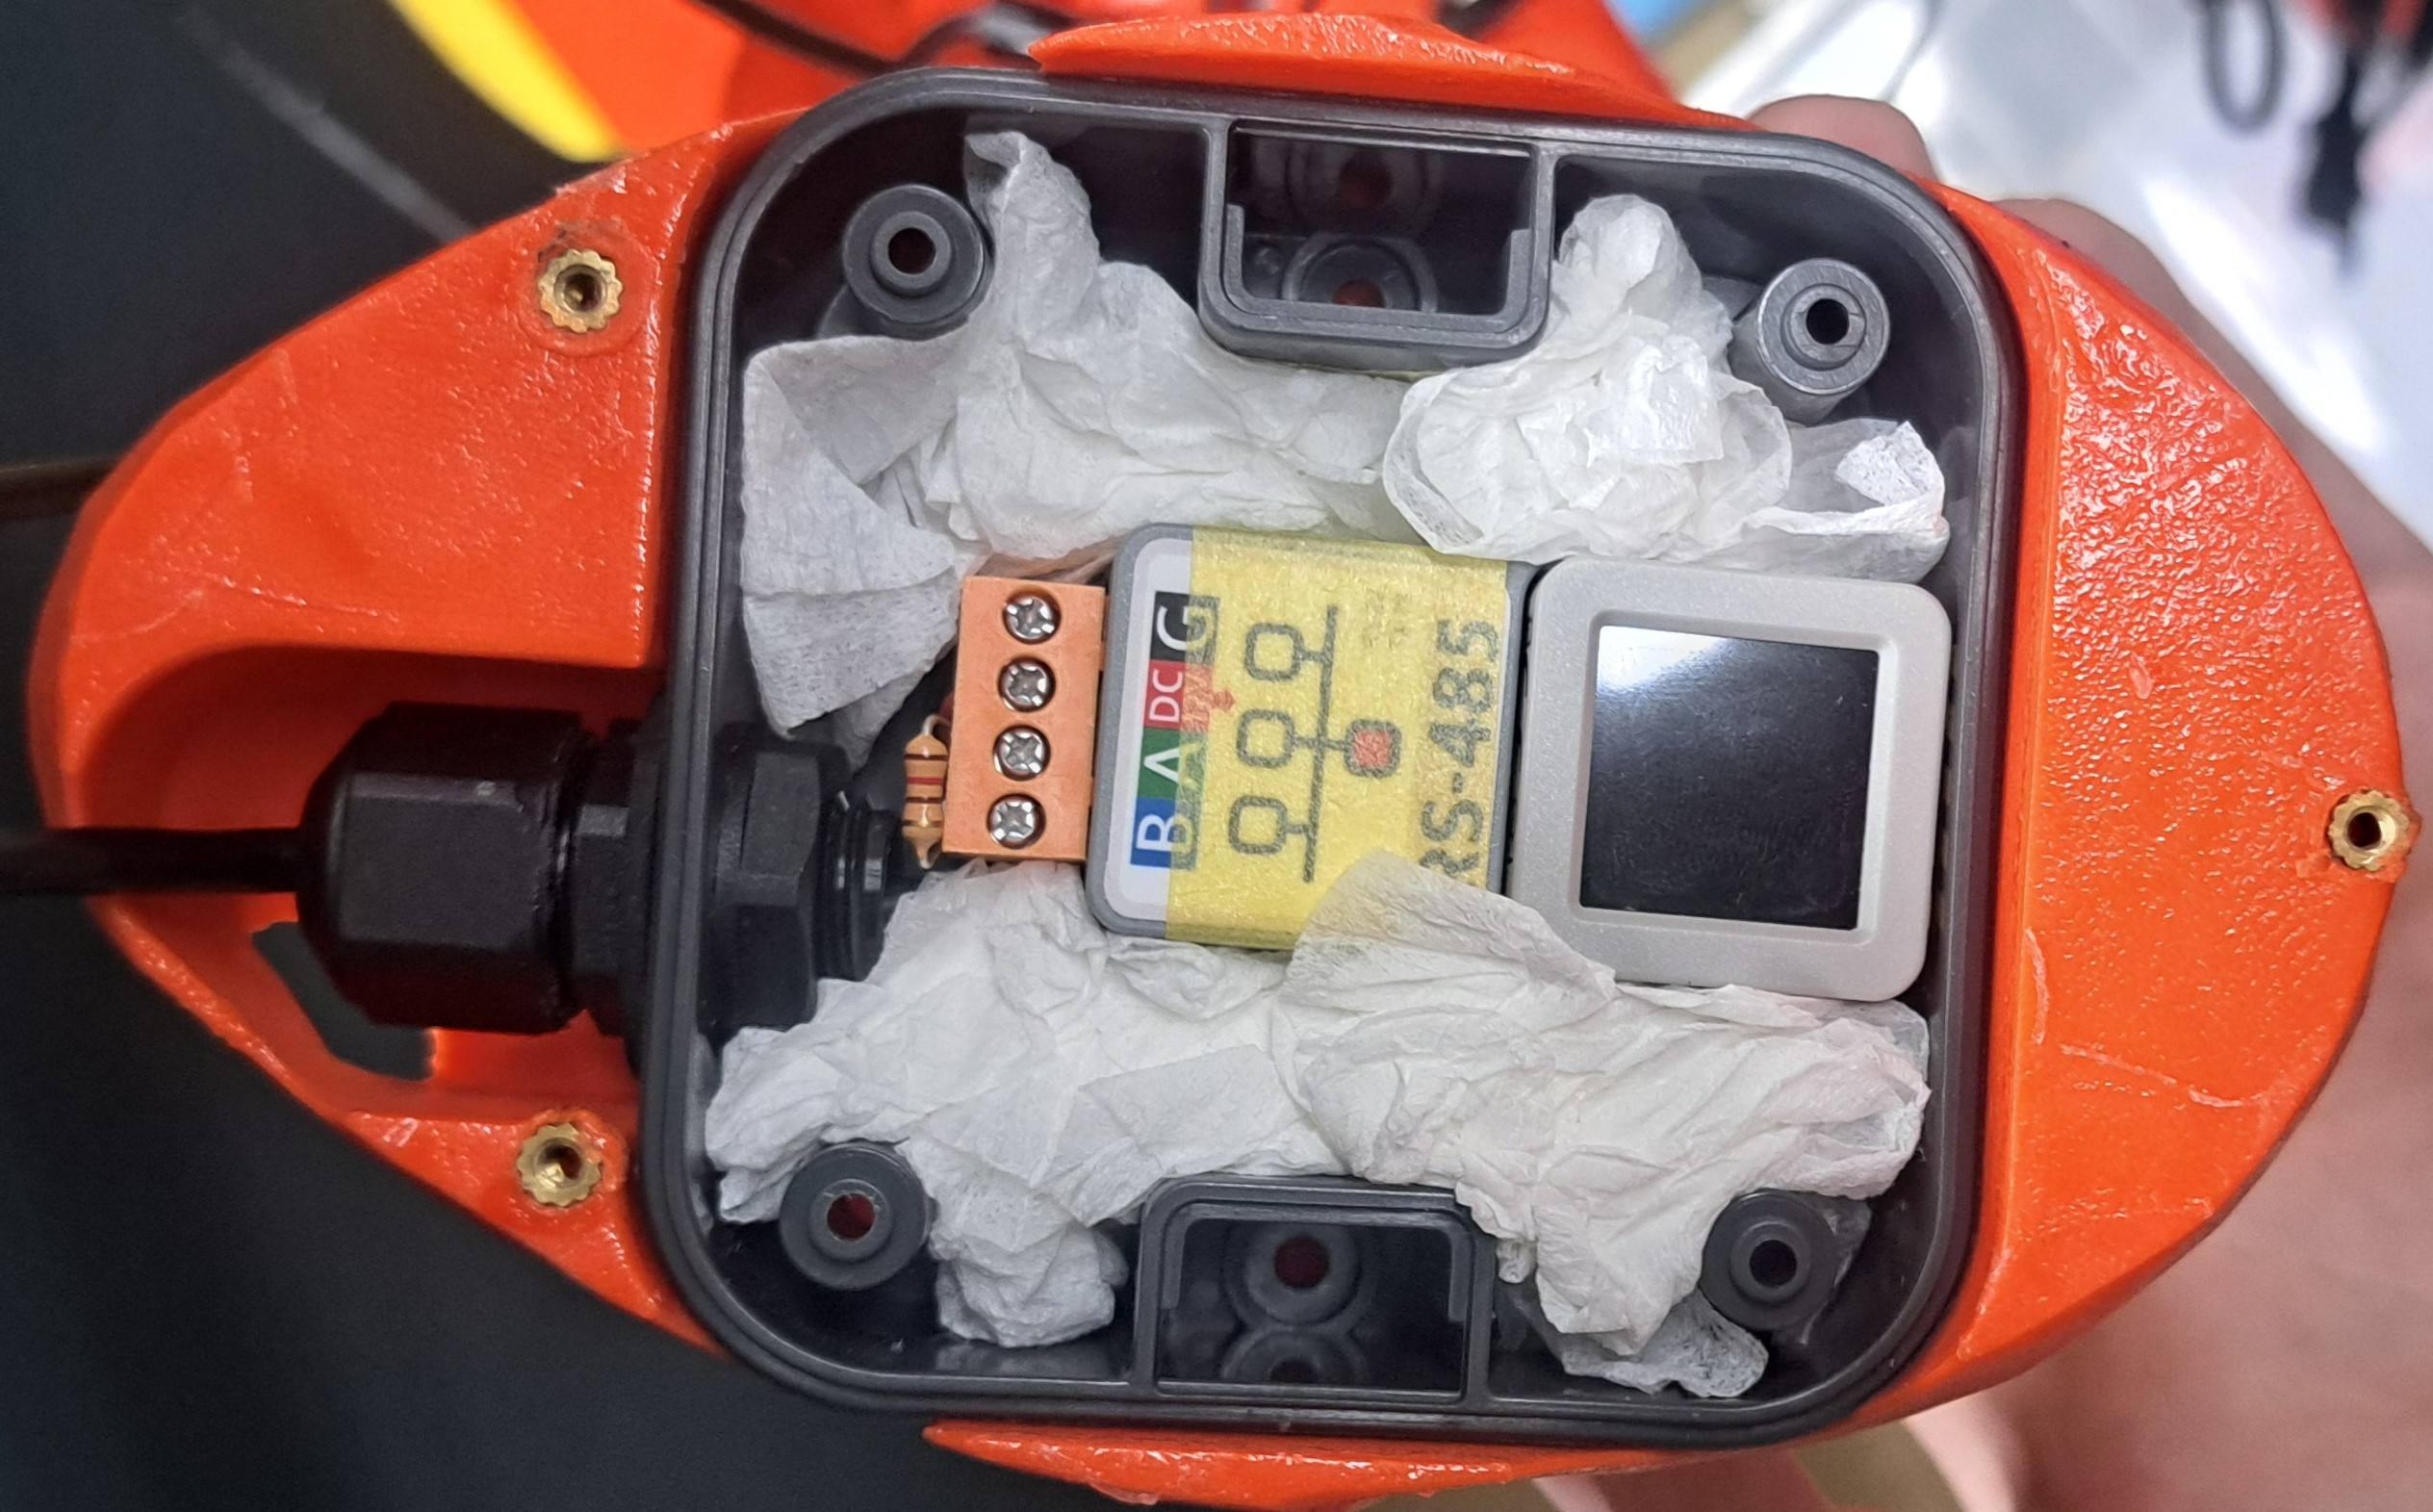
\includegraphics[width=0.6\textwidth]{Introduction/atoms3r_main_board.jpg}
    \caption{New main board for the SWUMANOID (housed in its head).}
    \label{fig:new_main_board_in_head}
\end{figure}

\subsubsection*{Running and optimizing the pool experiments}

To test the software that we developped during each week we put the robot in a real environment, so the second half of my mission plays out in the field, during pool experiments, about twice a week. These sessions follow a strict protocol to yield reliable data.The figure \ref{fig:pool_experiment} shows the robot going into the water during one of these tests.

\begin{figure}[H]
    \centering
    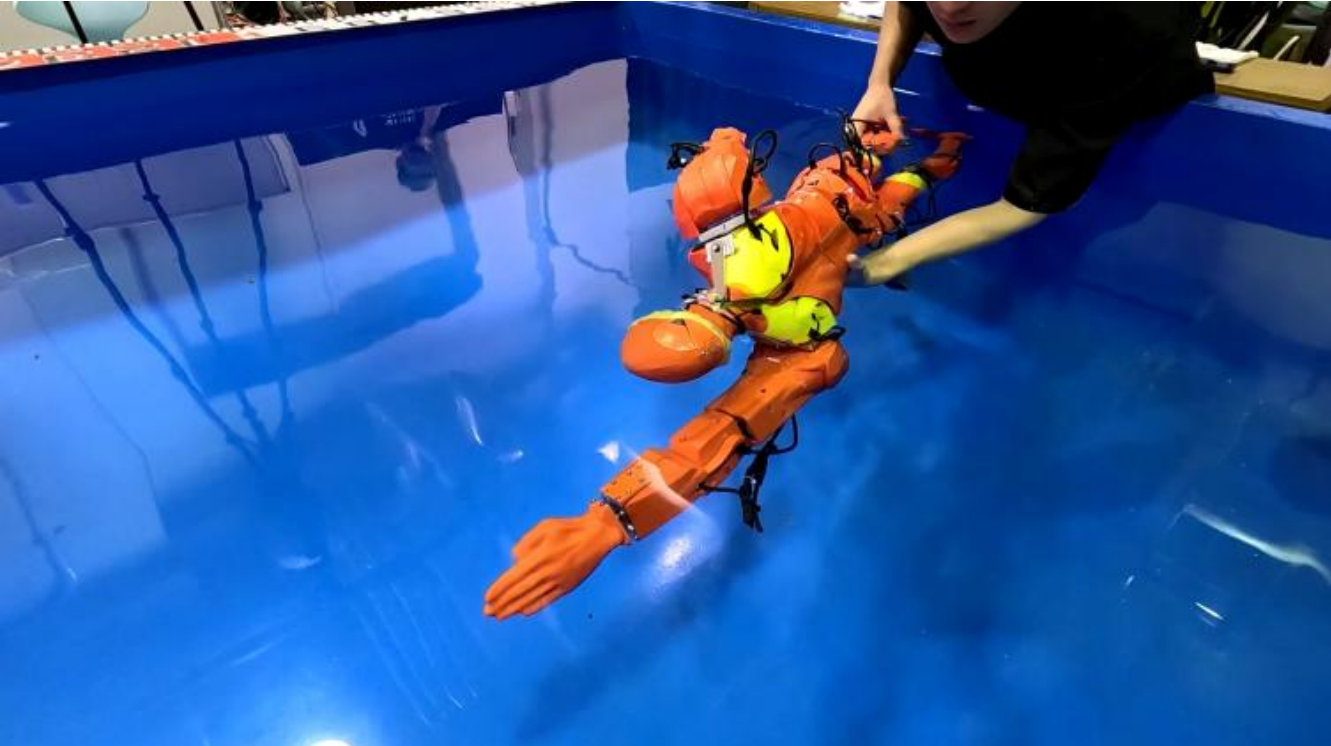
\includegraphics[width=0.7\textwidth]{Introduction/SWUMANOID_ready_to_swim_pool_room_experiment.png}
    \caption{Free-swimming pool experiment with the SWUMANOID.}
    \label{fig:pool_experiment}
\end{figure}

My job during these tests is to help the team prepare in the lab by weighing the robot, assembling the waterproof modules when needed, 3D-print parts for repairs or upgrades, and carrying the equipment to the pool. Once there, we set up the measurement system. That means laying measuring tapes along the water line to estimate the robot's spatial speed \cite{chung2013free}, configuring the control PC, and installing the tracking camera we need for the later kinematic analysis \cite{chung2013free}.

\begin{figure}[H]
    \centering
    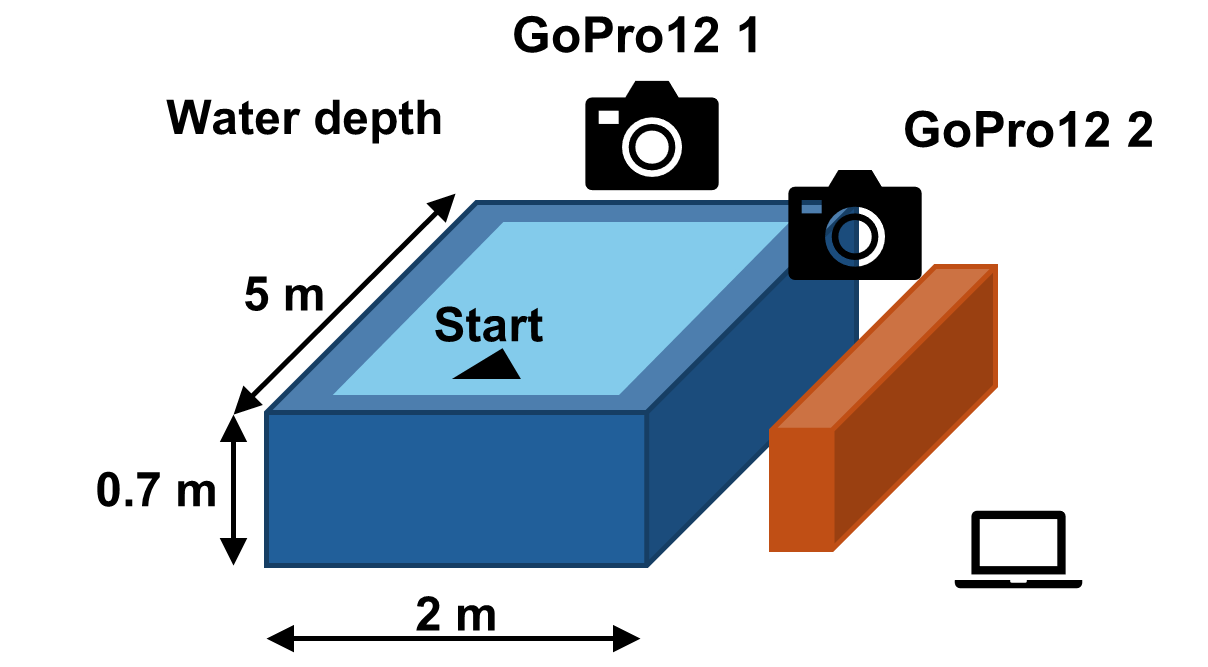
\includegraphics[width=0.6\textwidth]{Introduction/Salle_experience_dispositif.png}
    \caption{Layout of the experiment recording setup.}
    \label{fig:dispositif_experiment}
\end{figure}

During the experiment itself, I operate the SWUMANOID from the web interface I built. I swap trajectory files after each run and adjust control parameters like the sampling frequency or the stroke cycle time, testing different configurations to find the best trade-off between swimming speed and propulsive efficiency. In practice, these tests confirm the optimization models my supervisors compute in simulation \cite{nakashima2012optimizing}.


\section{Building a Web Interface for Control}
\label{sec:web_interface_sec}
\subsection{Code Migration and Getting Started}

When I joined the SWUMANOID project, my first big task was to take over and develop the firmware of the robot's embedded controller. On my first day, M. YANADORI and M. NAGATA handed me a set of requirements written during their earlier pool experiments, where they had spotted several critical weaknesses in the old control system.

As said in the previous section, the old microcontroller has some issues, in fact, the control frequency was locked at 72 Hz, which produced mechanical jerks, the Wi-Fi link dropped packets frequently and logging went to an SD card that turned out to be far too slow, sometimes stalling the main code. My overall goal, then, was to improve the robot's performance, stability, and user interface.

The embedded system is built on the \textbf{PlatformIO} build system, using the \textbf{Arduino} framework on an \textbf{Espressif ESP32-S3} microcontroller. The firmware handles real-time control of the servomotors over a Dynamixel RS-485 bus, inertial measurement, wireless communication through a Wi-Fi access point, and the reading of motion trajectories.

Originally, the software was built around a finite state machine driven by \textbf{UDP} commands received from a web interface, with the system state and telemetry sent back to the client through periodic packets. Inherited from earlier experiments, this scheme relied on a fixed-rate "burst" UDP stream, which was especially sensitive to Wi-Fi packet loss.

During the migration, I replaced this UDP stack with \textbf{HTTP}-based communication. The operator's commands (bus scan, load a motion, play, stop, E-STOP) now travel as simple HTTP requests, while the system state, motor telemetry and IMU data are streamed continuously to the browser over a one-way \textit{Server-Sent Events} (SSE) flow, which holds up far better against the small Wi-Fi dropouts.

The original firmware had been written and validated for the \textbf{M5Stack AtomS3} development board \cite{m5stack_atoms3}. But to meet the new requirements, the hardware had just been upgraded to the \textbf{M5Stack AtomS3R} \cite{m5stack_atoms3r} right before I arrived, we can see the two microcontrollers in the figure \ref{fig:m5stack_comparison}.

\begin{figure}[H]
    \centering
    \begin{subfigure}[b]{0.4\textwidth}
        \centering
        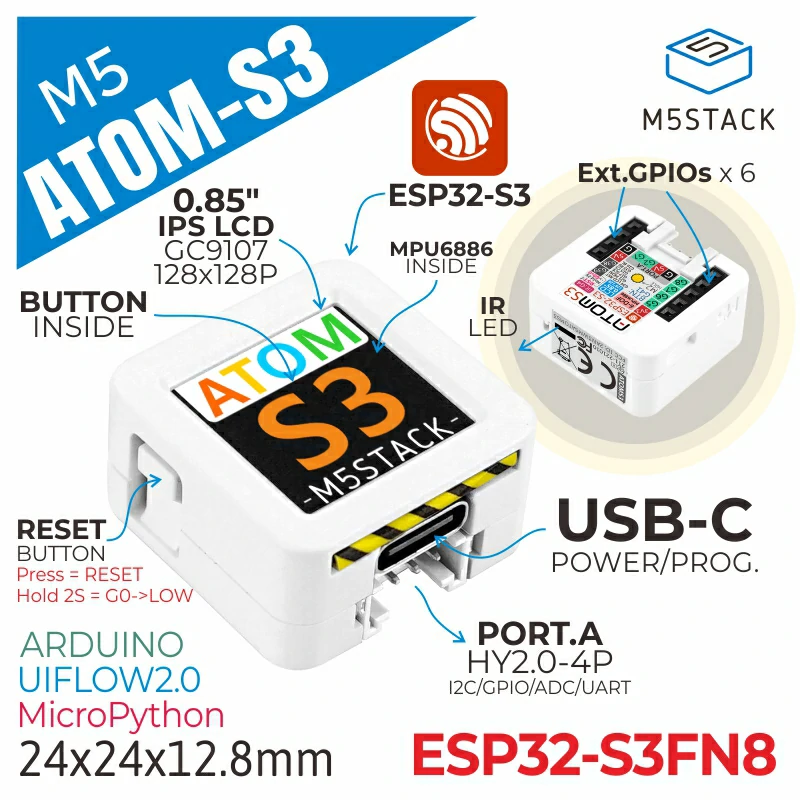
\includegraphics[width=\textwidth]{partie2/atoms3_picture.png}
        \caption{M5Stack AtomS3}
    \end{subfigure}
    \hfill
    \begin{subfigure}[b]{0.4\textwidth}
        \centering
        
\includegraphics[width=\textwidth]{partie2/atoms3r_picture.png}
        \caption{M5Stack AtomS3R}
    \end{subfigure}
    \caption{Visual and technical comparison of the two microcontrollers.}
    \label{fig:m5stack_comparison}
\end{figure}

Both boards share the same core architecture, the ESP32-S3 SoC, which gives them identical compute power and the same networking module (Wi-Fi/Bluetooth). They differ in how their chip is integrated and in their peripheral components. In fact, the AtomS3R uses a highly integrated "PICO" module that stacks extra memory without growing the board's footprint. The table \ref{tab:m5stack_diff} lays out all of these hardware characteristics.

\begin{table}[H]
\centering
\begin{tabular}{|l|l|l|}
\hline
\textbf{Characteristic} & \textbf{AtomS3} & \textbf{AtomS3R} \\
\hline
\textbf{SoC model} & ESP32-S3FN8 & ESP32-S3-PICO \\
\hline
\textbf{Processor} & \multicolumn{2}{c|}{Xtensa® dual-core 32-bit LX7 (up to 240 MHz)} \\
\hline
\textbf{Connectivity} & \multicolumn{2}{c|}{Wi-Fi 2.4 GHz \& Bluetooth 5.0 (LE)} \\
\hline
\textbf{Flash memory} & 8 MB & 8 MB \\
\hline
\textbf{External PSRAM} & None & \textbf{8 MB} \\
\hline
\textbf{IMU sensor} & MPU6886 (I2C 0x68) & BMI270 + BMM150 \\
\hline
\textbf{Backlight control} & Direct GPIO & I2C LED driver (AW9523) \\
\hline
\end{tabular}
\caption{Detailed hardware comparison between the AtomS3 and the AtomS3R \cite{m5stack_atoms3, m5stack_atoms3r}.}
\label{tab:m5stack_diff}
\end{table}

So the key advantage of the new microcontroller is the added \textbf{8 MB of PSRAM} on the AtomS3R \cite{m5stack_atoms3r} which allows to solve the problems my supervisors raised. Thanks to its dual-core processor and its large RAM reserve, the AtomS3R now lets us:
\begin{itemize}
    \item Reach an ultra-fast \textbf{200 Hz} control loop for all 21 motors, giving smooth, responsive motion free of mechanical jolts.
    \item Run the Wi-Fi network on core 0 of the processor, while core 1 handles only the motor control loop in a strictly deterministic way, never interrupted by network requests.
    \item \textbf{Eliminate the SD-card bottleneck}: the large PSRAM now lets us store all the telemetry logs extremely fast, directly in the microcontroller's RAM, before sending them to the web interface at the end of an experiment.
\end{itemize}

My first technical task, then, was to \textbf{migrate the hardware driver layer} from the old code to the new AtomS3R firmware. In fact, the original code relied on manual register access specific to the AtomS3, so I had to rework that part around the \textbf{M5Unified} library, which natively supports both hardware architectures. I started by replacing the raw I2C register access (specific to the MPU6886) with standardized \texttt{M5.Imu} calls to correctly read the new BMI270 sensor, then I made sure the LCD screen and its new I2C backlight controller were properly initialized during the \texttt{Boot} sequence.


\subsection{New Web Architecture}
The main goal of this second development phase was to fold every control function directly into the user interface, the page that manages the microcontroller, so we could drive the SWUMANOID correctly and easily. Just as important, the interface had to show, in real time, all the information we need to run the experiments well and to understand which factor is limiting us and how to fix it.

The starting point was a minimal supervision console (figure~\ref{fig:evolution_rssi}, left), limited to a raw display of the controller state and a few text commands. It told us nothing about the radio link quality, the robot's actual orientation, or the state of individual actuators, which made any experimental diagnosis painful. So the rework was done incrementally, each iteration adding a measurement instrument aimed at one limiting factor identified during the tests.

\begin{figure}[H]
    \centering
    \begin{subfigure}[b]{0.48\textwidth}
        \centering
        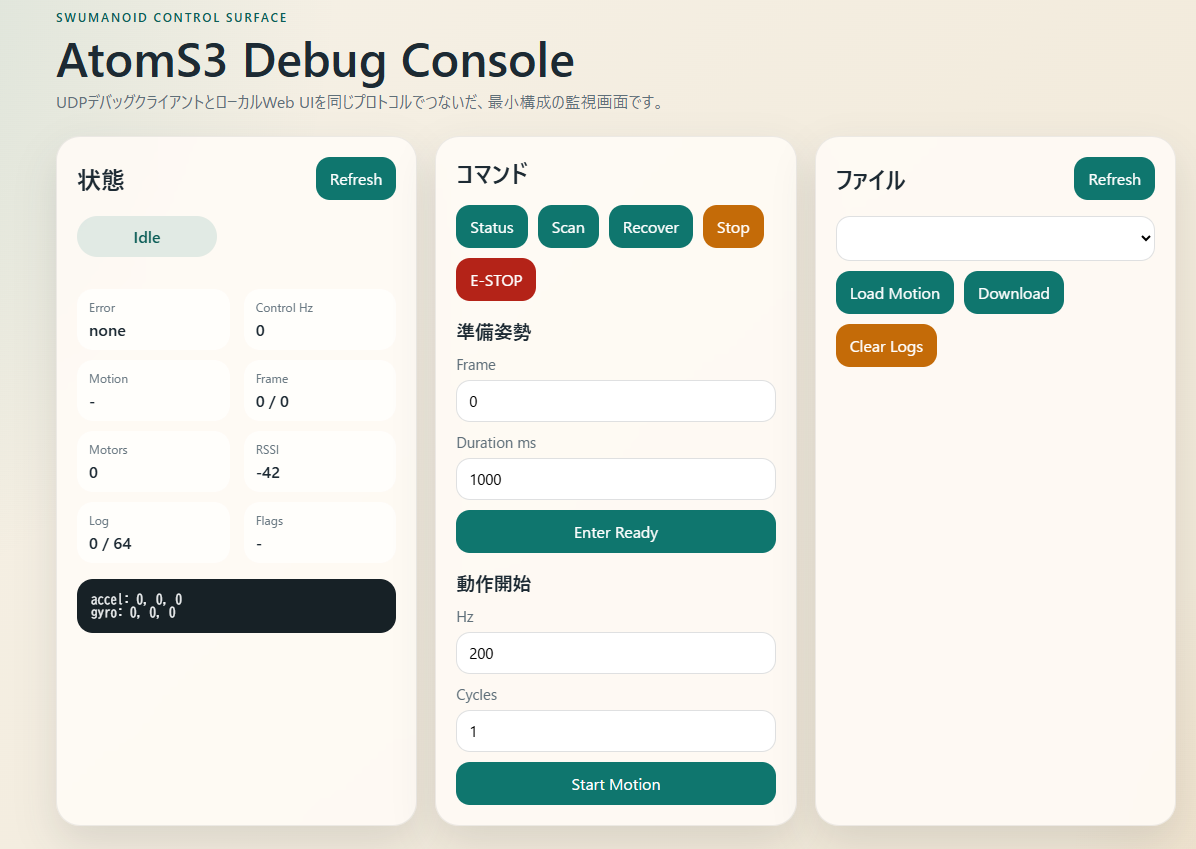
\includegraphics[width=\textwidth]{Interfaces/0_old_interface_begining.png}
        \caption{Initial console for the AtomS3.}
        \label{fig:old_interface}
    \end{subfigure}
    \hfill
    \begin{subfigure}[b]{0.48\textwidth}
        \centering
        
\includegraphics[width=\textwidth]{Interfaces/1_change_RSSI_log.png}
        \caption{Adding the real-time RSSI plot.}
        \label{fig:rssi_chart}
    \end{subfigure}
    \caption{Evolution of the supervision interface.}
    \label{fig:evolution_rssi}
\end{figure}

Since the requirements stressed that the Wi-Fi is often unstable, that's why I started to implement a network diagnostic system:
\begin{itemize}
    \item I modified the firmware to compute the \textbf{RSSI} (Received Signal Strength Indicator), the actual strength of the Wi-Fi signal as seen by the robot.
    \item I built a web control interface with a \textbf{real-time chart (via Chart.js~\cite{chartjs})} that plots how this signal evolves. It lets us locate the packet-loss zones and confirm the connection quality before sending the robot into the water.
\end{itemize}

In practice, the firmware samples the RSSI at the same rate as the real-time telemetry stream ($\approx 20$~Hz) and exposes it to the client, which feeds a thirty-second sliding window. The resulting curve (Figure~\ref{fig:evolution_rssi}, right) gives us a measurable, usable quantity to map the link range around the pool.


In the same spirit, I added a three-dimensional avatar of the robot to the interface, rendered in the browser with the Three.js library~\cite{threejs}. This mannequin reproduces, in real time, the spatial orientation measured by the inertial unit (IMU) housed in the AtomS3R's head. The operator gets an immediate read of the SWUMANOID's attitude (roll, pitch, yaw) without having to interpret raw numbers (Figure~\ref{fig:imu_avatar}). The full inertial signal processing chain and the orientation angle computation have their own section (see \ref{sec:calcul_angle}), but here I only want to underline the role of this visualization as a qualitative control instrument during an experiment.

\begin{figure}[H]
    \centering
    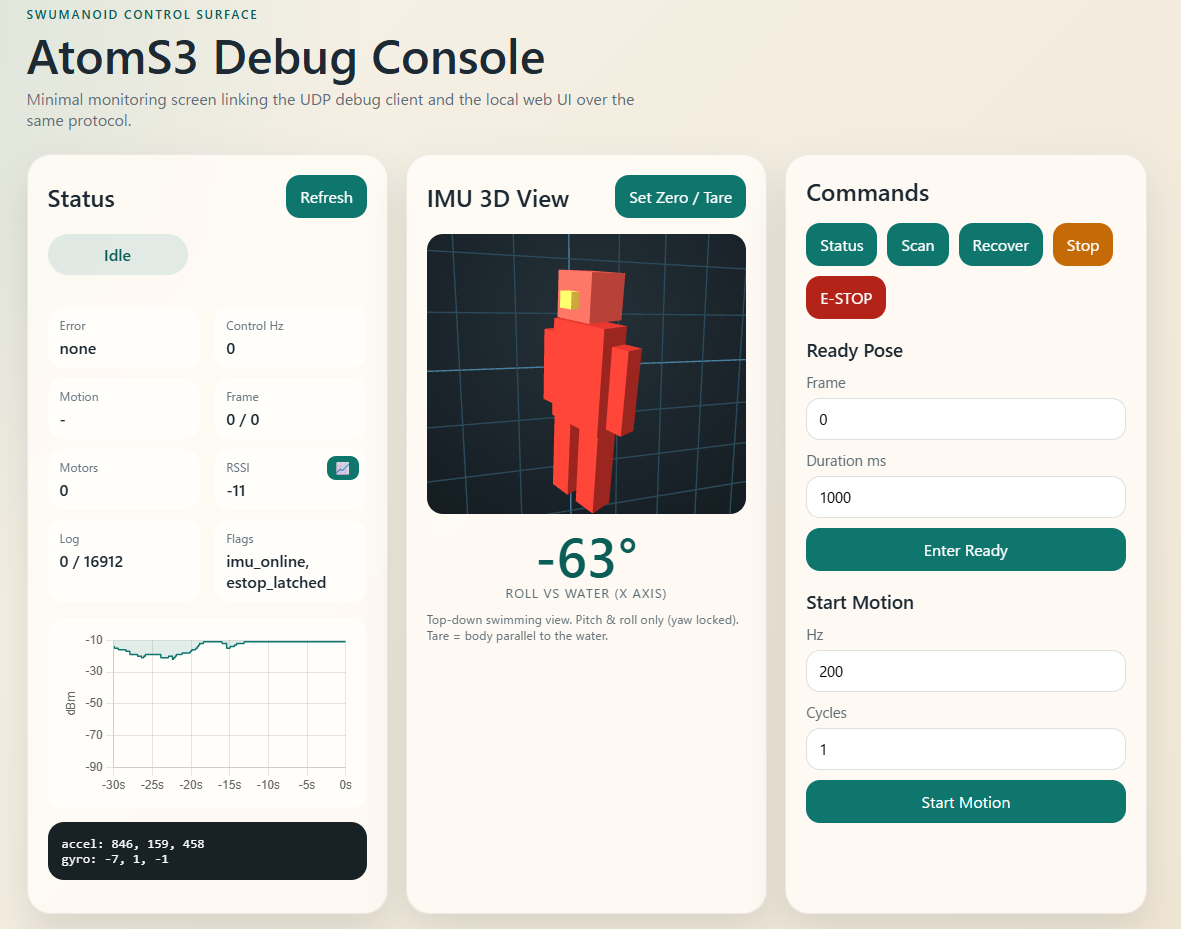
\includegraphics[width=0.6\textwidth]{Interfaces/2_change_3D_Visualisation_with_angle.png}
    \caption{Web interface with the 3D IMU avatar.}
    \label{fig:imu_avatar}
\end{figure}

I also added the ability to upload motion files straight from SWAM (.dat), converted on the fly during upload, to make the web control interface fully standalone, smooth and secure. The trajectory conversion logic runs entirely on the client (JavaScript) and I ported it from the MATLAB code used previously and provided by Iroki-san.

More precisely, when parsing the \texttt{.dat} file in JavaScript, each joint angle is converted to Dynamixel ticks using the affine formula of the X-series motors~\cite{dynamixel_x_manual}:
\begin{equation}
tick = \frac{\theta_{deg}+180}{360} \times 4095
\end{equation}
The conversion includes an integer rounding and a clamp to $[0, 4095]$. It can also apply a per-servo calibration table (an offset and rotation direction specific to each joint), to compensate for the mechanical mounting differences between the model's theoretical axis and the actuator's real axis. 

Also, as we will discuss in section \ref{sec:method_interpolation}, we decided to make the control frequency and the duration of a swimming cycle user-configurable to allow for flexible robot control. This capability entails calculating a new number of frames, $F$, using an interpolation method explained later and resulting in a frame count that differs from that of the motion file originally uploaded to the client.

Finally, the AtomS3R now acts as a simple executor, it indeed receives the trajectory as a single compact binary block, which makes it immune to Wi-Fi instability during playback. This binary format (little-endian) drastically minimizes the network transfer size, the structure of this packet is detailed in Table \ref{tab:binary_payload}.

\begin{table}[h]
\centering
\begin{tabular}{|c|c|l|}
\hline
\textbf{Offset} & \textbf{Type} & \textbf{Content} \\ \hline
0 & \texttt{uint8} & Version ($=1$) \\ \hline
1 & \texttt{uint8} & Number of motors $N$ \\ \hline
2-5 & \texttt{uint32} & Number of frames $F$ \\ \hline
6 to $5+N$ & $N \times \texttt{uint8}$ & Motor IDs (column order) \\ \hline
$6+N$ to end & $F \times N \times \texttt{uint16}$ & Ticks (row-major) \\ \hline
\end{tabular}
\caption{Structure of the binary trajectory packet sent through the API}
\label{tab:binary_payload}
\end{table}

The total payload size (in bytes), noted $S$, depends directly on the number of motors $N$ and the number of frames $F$. From the structure in Table \ref{tab:binary_payload}, the generic formula breaks down as:
\begin{equation}
S(N, F) = 6 + N + 2NF
\end{equation}
where $6$ bytes are the fixed header (Version, Number of motors, Number of frames), $N$ bytes hold the motor ID array, and $2NF$ bytes carry the raw trajectory data (each position coded on an unsigned 16-bit integer, so 2 bytes).\\

In our setup, the SWUMANOID is driven by $N = 21$ motors. For a trajectory of $F = 144$ frames, the exact network transfer size is:
\begin{align*}
S(21, 144) &= 6 + 21 + 2 \times 21 \times 144 \\
S(21, 144) &= 27 + 2 \times 3024 \\
S(21, 144) &= 27 + 6048 \\
S(21, 144) &= 6075 \text{ bytes}
\end{align*}

With a network \textit{payload} of exactly 6075 bytes (about 6.07 kB), the AtomS3R can easily absorb the whole trajectory in a single transfer. This loading panel also exposes the playback timing settings (rate in Hz, cycle duration, number of repetitions), from which the number of resampled frames is recomputed (Figure~\ref{fig:motion_control}). The web interface was reorganized into five vertical panels (Status, Network \& Scan, IMU Lab, Motion Control, Motion Settings \& Logs) for better readability and the real-time communication now relies on one-way \textit{Server-Sent Events} (SSE)~\cite{whatwg_sse} rather than WebSockets, which removes the jitter and collision problems on the RS-485 bus.

\begin{figure}[H]
    \centering

    \begin{subfigure}[b]{0.5\textwidth}
        \centering
        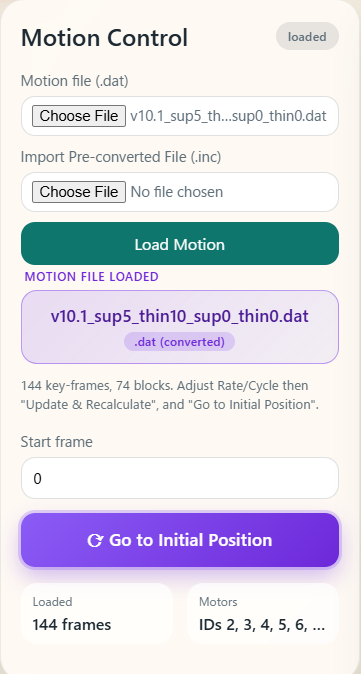
\includegraphics[width=0.42\textwidth]{Interfaces/4_motion_control.png}
        \caption{\emph{Motion Control} panel.}
        \label{fig:motion_control}
    \end{subfigure}
    \hfill
    \begin{subfigure}[b]{0.35\textwidth}
        \centering
        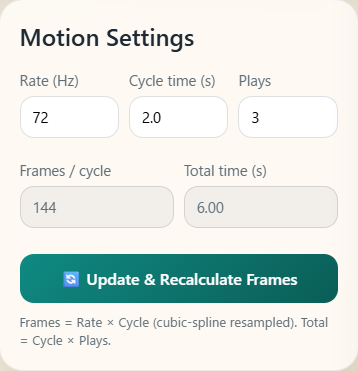
\includegraphics[width=\textwidth]{Interfaces/4_motion_settings.png}
        \caption{\emph{Motion Settings} panel.}
        \label{fig:motion_settings}
    \end{subfigure}
    \caption{\emph{Motion Control} and \emph{Motion Settings} panels with motion file upload.}
\end{figure}

To check the integrity of the actuation chain before any motion, I also implemented an \textbf{RS-485 bus scan}. On the operator's command, the firmware pings (Dynamixel 2.0 \textit{ping}) the whole configured ID range and keeps only the motors that answered. For each of them, it reads the control table to report supply voltage, instantaneous current, temperature and the hardware error register (Figure~\ref{fig:scan_motors}). At a glance, the operator sees how many motors are actually online on the bus and their state of health, which avoids starting an experiment with a faulty or disconnected actuator. Since this read blocks the control loop (missing IDs cause a \textit{timeout}), it is triggered explicitly and never during motion playback.

\begin{figure}[H]
    \centering
    \begin{subfigure}[b]{0.46\textwidth}
        \centering
        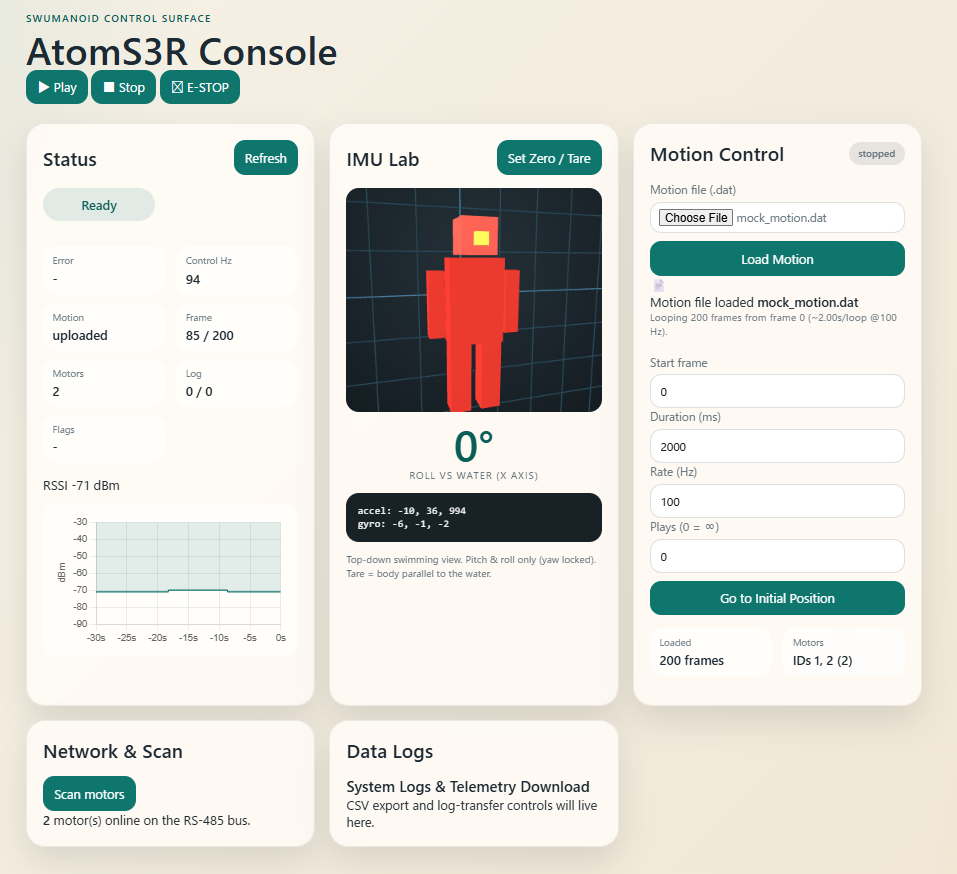
\includegraphics[width=\textwidth]{Interfaces/3_scan_motors.png}
        \caption{\emph{Network \& Scan} panel in the dashboard.}
        \label{fig:scan_panel}
    \end{subfigure}
    \hfill
    \begin{subfigure}[b]{0.3\textwidth}
        \centering
        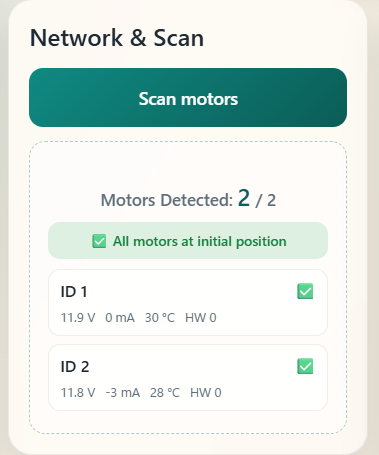
\includegraphics[width=\textwidth]{Interfaces/3_scan_motors_example.png}
        \caption{Result after a scan.}
        \label{fig:scan_result}
    \end{subfigure}
    \caption{RS-485 bus scan feature.}
    \label{fig:scan_motors}
\end{figure}

All of these instruments were put into a single dashboard (Figure~\ref{fig:final_dashboard}), which gathers on one view the controller state and MCU temperature, the network scan panel, the IMU lab (3D avatar and roll, yaw, pitch angles), the motion control, and the telemetry management described in the next section.

\begin{figure}[H]
    \centering
    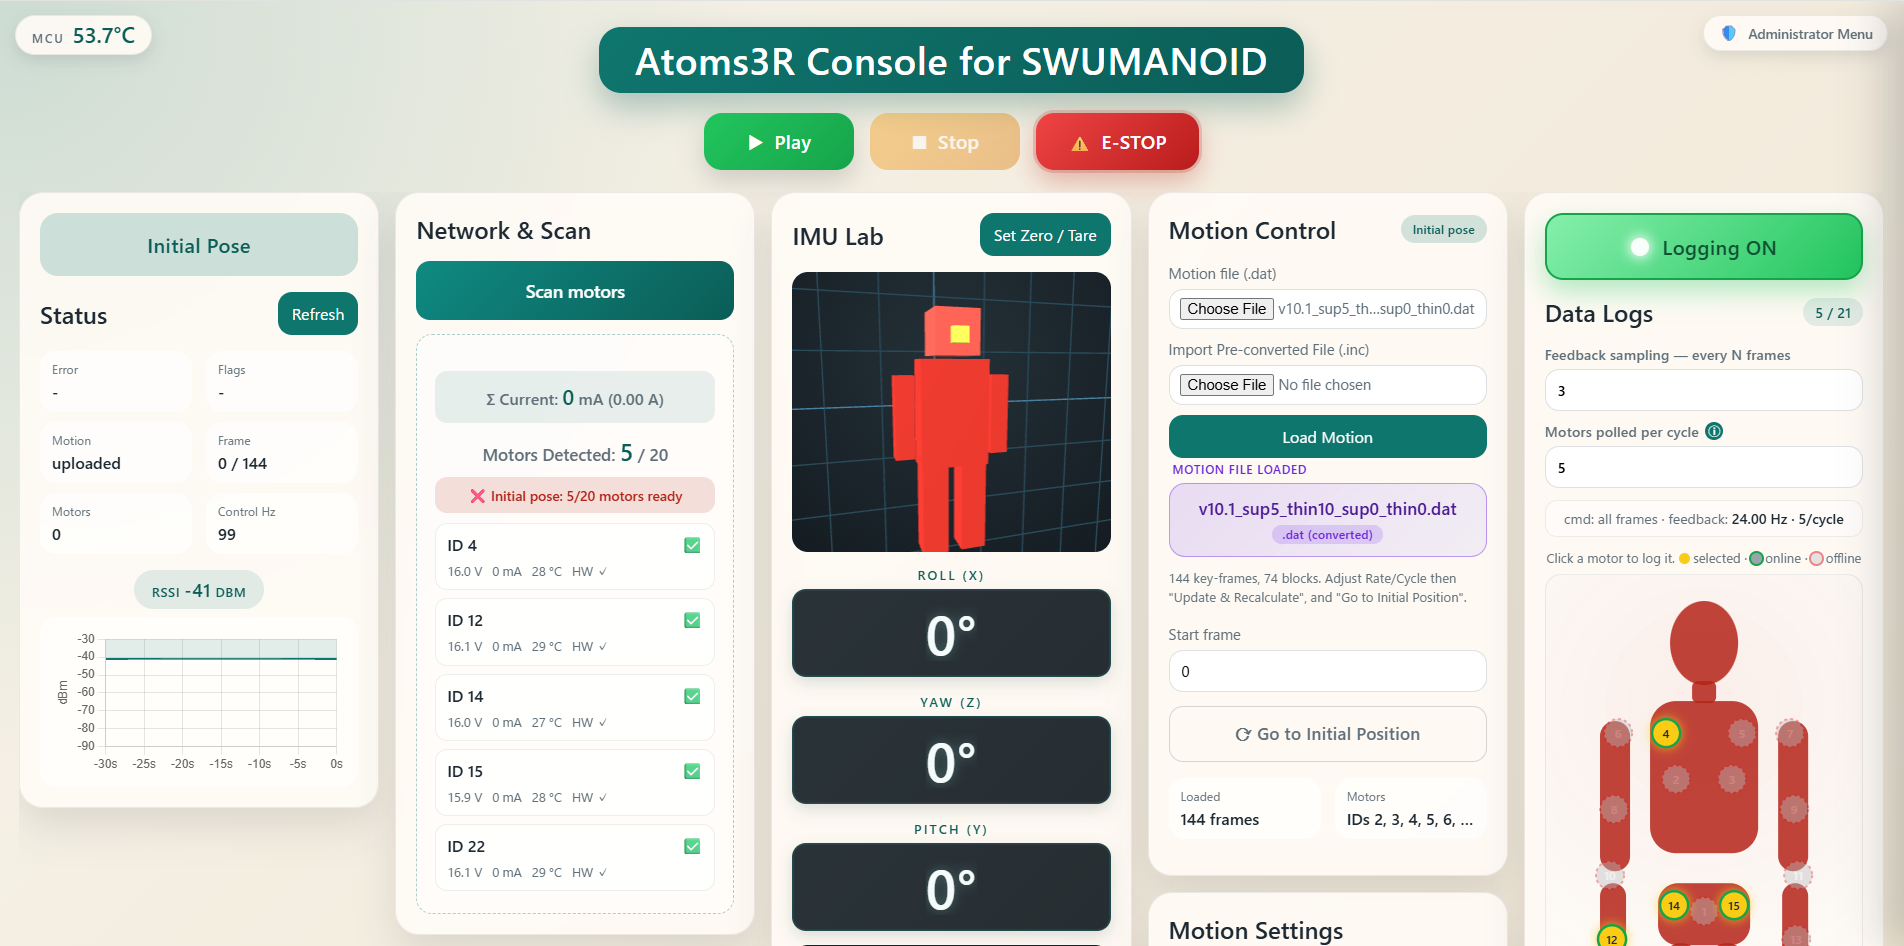
\includegraphics[width=0.75\textwidth]{Interfaces/6_final_interface_with_angles_roll_yaw_pitch.png}
    \caption{Final control dashboard of the SWUMANOID.}
    \label{fig:final_dashboard}
\end{figure}

Across the pool experiments, the small Wi-Fi dropouts would often freeze the web interface without warning the user. To make the system resilient to signal loss, I wrote a JavaScript \textit{Watchdog} that monitors the \textit{Server-Sent Events} (SSE) stream, so if no data arrives for 600 ms, the interface shows an "OFFLINE" alert and silently attempts to reconnect. The reconnection strategy is \emph{linear} and aggressive, with fixed, closely spaced retries, because underwater the Wi-Fi link drops the instant the robot goes under and only comes back when it surfaces. It's allowing the fact to not have any waiting delay once the robot reappears.


\subsection{Telemetry Implementation and Memory Management}

In parallel, I wanted to add the ability to record the telemetry logs (position, current, voltage, IMU) of each run. The first problem I spotted was the risk of saturating the ESP32's RAM (PSRAM) if it had to generate and store a text file in CSV format. So the solution was to record these logs as a raw binary buffer, extremely compact. The software structure of one log cycle was optimized as shown in Table \ref{tab:telemetry}.

\begin{table}[h]
\centering
\begin{tabular}{|l|c|l|}
\hline
\textbf{Field} & \textbf{Type} & \textbf{Description} \\ \hline
\texttt{t\_us} & \texttt{uint32} & Timestamp in microseconds \\ \hline
\texttt{accel[3], gyro[3]} & $6 \times \texttt{int16}$ & IMU (milli-g, deci-deg/s) \\ \hline
\texttt{cmd, pos, cur} & \texttt{int16, int32, int16} & Command, Position, Current \\ \hline
\texttt{volt} & \texttt{uint16} & Voltage \\ \hline
\end{tabular}
\caption{Structure of the binary telemetry log record}
\label{tab:telemetry}
\end{table}

This choice allows to decouple the writing (a plain memory copy of fixed-width fields, with no allocation or text formatting) from the heavy processing, pushed offline onto the client computer. It also cleanly separates the command (\texttt{cmd}, known every cycle without touching the bus) from the position measurement (\texttt{pos}, acquired only when the motor actually answered). But during the first attempts to record all 21 motors, a drastic drop in the control frequency appears. The robot's motion became strongly jerky, causing frame loss and a degraded swimming dynamic. This was not a memory saturation problem, but the physical limit of the RS-485 communication bus running in \textit{half-duplex}.

%When a position could never be read, the field gets a sentinel value ($\mathtt{0x80000000}$) rather than zero. On the browser side, the matching CSV cell is then left empty, which prevents a zero or a leftover from the previous run from being mistaken for a valid physical reading.



While sending commands (\texttt{SyncWrite}) is nearly instant thanks to its \textit{broadcast} mode, reading states (\texttt{SyncRead}) forces each motor to answer sequentially. And with an individual response time of about 3 to 4 ms per motor, polling every actuator in one pass froze the control loop for 60 to 80 ms, far beyond the critical 10 ms budget of a 100 Hz control loop. To resolve this timing conflict between motion smoothness and data acquisition, the architecture was reworked like it :
\begin{itemize}
    \item \textbf{Spatial selection (UI):} I added an interactive SVG diagram of the robot to the web interface, letting the user click on joints to select only the relevant motors ($N$ motors instead of all 21 every time).
    \item \textbf{Temporal selection and smoothing:} The embedded code now separates command sending from sensor reading. The user can set a sampling stride (\textit{Feedback sampling every $K$ frames}) to avoid logging every single frame. On top of that, a rotating (\textit{Round-Robin}) read was introduced (\textit{Motors polled per cycle}) so only a small subgroup of motors is queried per clock cycle, capping bus occupancy at $\approx 7$ ms and preserving the integrity of the control loop.
\end{itemize}

\begin{figure}[H]
    \centering
    \begin{subfigure}[b]{0.21\textwidth}
        \centering
        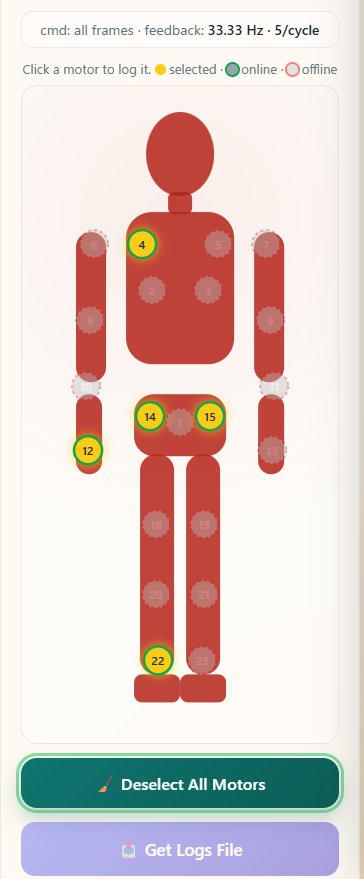
\includegraphics[width=\textwidth]{Interfaces/5_logs_svg_scheme.png}
        \caption{Interactive SVG diagram of the robot.}
        \label{fig:svg_scheme}
    \end{subfigure}
    \hfill
    \begin{subfigure}[b]{0.55\textwidth}
        \centering
        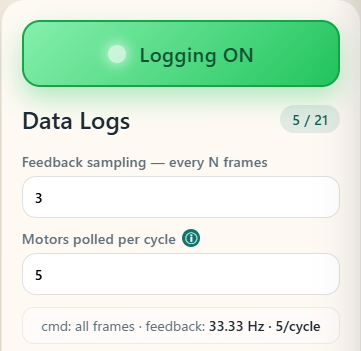
\includegraphics[width=\textwidth]{Interfaces/5_logs_example_sampling.png}
        \caption{Temporal selection of the logs}
        \label{fig:sampling}
    \end{subfigure}
    \caption{Tuning the telemetry acquisition.}
    \label{fig:svg_selection}
\end{figure}

On the figure~\ref{fig:svg_selection}, the SVG diagram turns each joint into a clickable dot whose color reflects the motor state (selected, online, offline). The list of chosen IDs becomes the \texttt{read\_ids} parameter passed to the firmware when the motion starts. On the embedded side, a round-robin cursor walks this list and, at each acquisition cycle, issues a single \texttt{SyncRead} over a subgroup of $G$ motors (\textit{Motors polled per cycle}). Since the command is logged every control period without any bus access, only the measured part is subject to this sequencing, so the result is an effective refresh rate, per motor, of the position measurement:
\begin{equation}
f_{fb} = \frac{f_{play}}{K \times \left\lceil \dfrac{N}{G} \right\rceil}
\end{equation}
where $f_{play}$ is the playback rate, $K$ the sampling stride (\textit{feedback every $K$ frames}), $N$ the number of selected motors and $G$ the subgroup width polled per cycle. These two variables allow us to trade telemetry density against motion smoothness, without ever letting the bus occupancy exceed $t_{bus} \approx G \times 4~\text{ms}$.


%This setup is rounded out by monitoring the safety-critical quantities. The current drawn by each motor, its supply voltage and its temperature are read during the bus scan (previous section), the total bus current is aggregated continuously, and the microcontroller's own temperature is shown permanently on the dashboard. These indicators let us catch a joint overheating or an abnormal current draw early, the classic symptom of a mechanical jam under hydrodynamic load, before it turns into a hardware failure.

So thanks to this temporal and structural organization, the \textit{stride} per record is reduced to $16 + 10N$ bytes. The total RAM size of the binary buffer, noted $M$, therefore depends on the number of selected motors $N$, the total number of frames $F$ of the trajectory, and the sampling interval $K$ (one frame recorded every $K$ frames). The generic formula is:
\begin{equation}
M(N, F, K) = \left\lfloor \frac{F}{K} \right\rfloor \times (16 + 10N)
\end{equation}

To estimate the memory load in the most demanding scenario (full recording with no selection and no subsampling), take $N = 21$ motors, clocked at 72 Hz over 2 seconds, so $F = 144$ frames, recording every frame ($K = 1$):
\begin{align*}
M(21, 144, 1) &= 32544 \text{ bytes}
\end{align*}

Even in this worst case, the buffer needs only $\approx 32.54 \text{ kB}$ of RAM, entirely negligible next to the 2 MB allocated on the chip. At the end of a run, this compact binary block is transferred to the web browser and then the JavaScript on the client computer decodes the binary, builds the full \texttt{.csv} text file, and automatically triggers the offline download for the user.


\section{Motor Tests and Main Board Configuration}
\label{sec:motors_board_configuration}

\subsection{Building a First Circuit and the Need for New Components}

To validate the RS-485 communication chain (Dynamixel 2.0 protocol) between the microcontroller and the actuators, a preliminary hardware test bench was established. Due to the initial unavailability of the SWUMANOID's waterproof XW-series motors, functionally equivalent XM-series motors (XM430 and XM540-W150-R~\cite{dynamixel_xm540w150}) were utilized. These actuators share the same electrical and protocol properties, making them a representative substitute for tuning the communication layer.

Initial single-motor tests with minimal wiring successfully validated basic commands (\textit{Ping}, \textit{Torque Enable}), exhibiting a negligible $2\%$ packet loss with no impact on motion precision. However, scaling to a multi-motor configuration required a rigorous electrical topology to maintain signal integrity and ensure device detection (Figure~\ref{fig:premier_circuit}):
\begin{itemize}
\item \textbf{Power supply (Star topology)}: Independent 12\,V and ground lines for the microcontroller and each motor, connected to a strict common ground to prevent voltage drops and ground loops.
\item \textbf{Data line (Daisy-chain)}: Series routing of the D+ (A) and D-- (B) signals across the devices.
\end{itemize}

\begin{figure}[H]
\centering
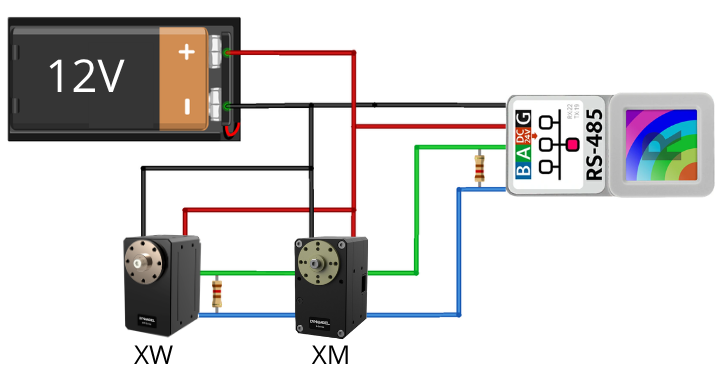
\includegraphics[width=0.65\textwidth]{schemas/First_test_schema_xm_xw_motors.png}
\caption{Diagram of the first test circuit.}
\label{fig:premier_circuit}
\end{figure}

Despite this topology, the bus experienced an $80\%$ packet loss, causing severe motion instability. The problem could be a signal reflection in an unterminated differential bus so to achieve impedance matching and absorb these reflections, 120\,$\Omega$ termination resistors~\cite{dynamixel_x_manual} were installed at both ends of the transmission line (at the AtomS3R base and the terminal motor). While this hardware correction successfully eliminated signal interference, attempting to scale the control frequency exposed a critical bottleneck, as illustrated in the figure~\ref{fig:first_bad_result}, commanding the motors at 90\,Hz led a real control rate capped at only 73.8\,Hz. Furthermore, the actuator exhibited severe tracking latency, with the physical position significantly lagging behind the commanded trajectory. Such degraded responsiveness and time stretching are entirely incompatible with the precision required for hydrodynamic pool experiments.

\begin{figure}[H]
\centering
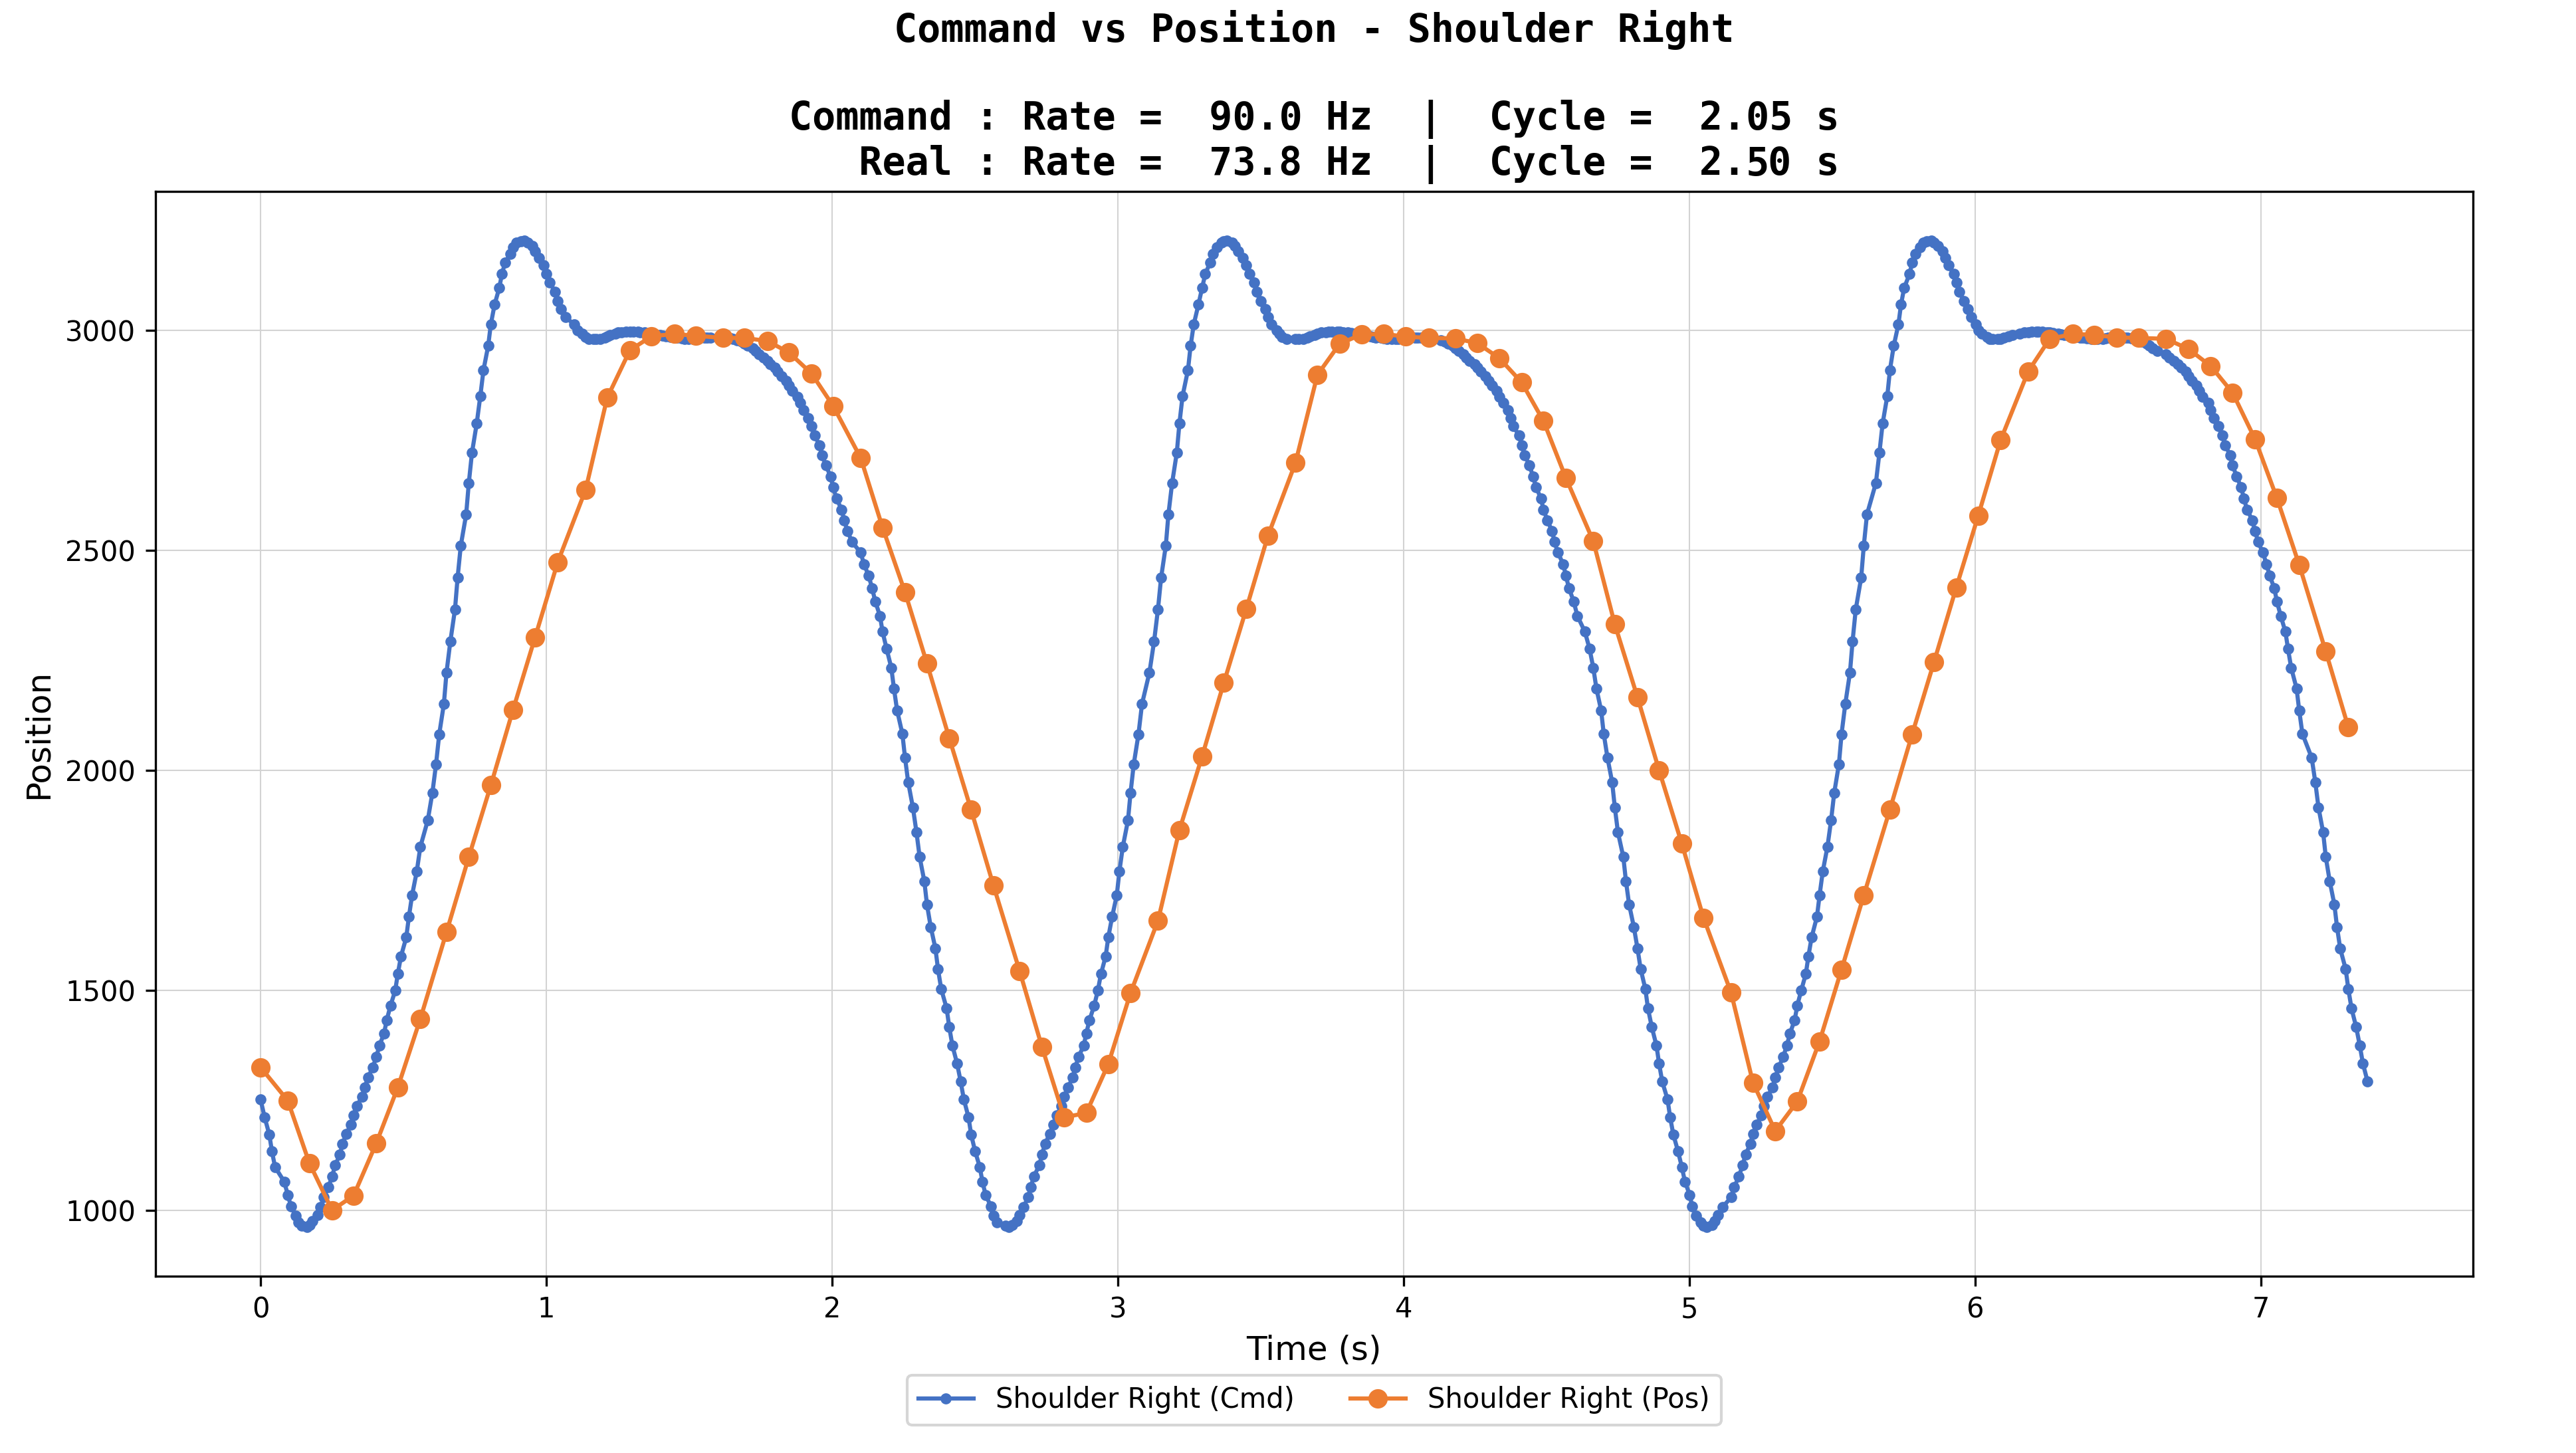
\includegraphics[width=0.85\textwidth]{graphiques/First_result_bad_control_ID_4.png}
\caption{Command versus actual position of the right shoulder at a 90\,Hz setpoint.}
\label{fig:first_bad_result}
\end{figure}

To achieve the 200\,Hz control frequency target, the bus throughput needed to reach at least 1 Mbps. However, initial tests revealed a physical transmission cap at 115200 bps, beyond which the microcontroller failed to detect the motors. This limitation did not originate from the SP3485 transceiver~\cite{sp3485}, which supports up to 10 Mbps, but rather from the automatic direction circuit of the \textit{Atomic RS485} base~\cite{m5stack_atomic485}.

Because the Dynamixel bus operates in half-duplex, a single A/B wire pair for both directions, the transceiver must constantly switch between transmit and receive modes via its Driver Enable (DE) pin, but the \textit{Atomic RS485} base does not expose this pin, relying instead on an internal automatic circuit to guess the data direction. While functional at low speeds, where a single bit lasts roughly 8.7 µs, this automatic switching is too slow for a 1 Mbps throughput, where a bit lasts $\approx 1$ µs. Consequently, the circuit fails to release the line fast enough, masking the start of the motor's \textit{Status Packet} reply. This turnaround latency previously required a deliberately high \textit{Return Delay Time} ($\approx 500$ µs)~\cite{dynamixel_x_manual}, a workaround incompatible with high-frequency control loops.

\begin{figure}[H]
    \centering
    \begin{subfigure}[b]{0.25\textwidth}
        \centering
        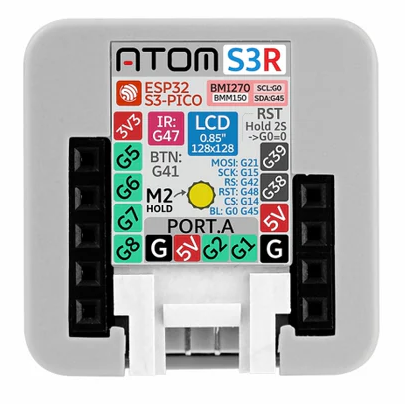
\includegraphics[width=\textwidth]{composants/atoms3r_pinout.png}
        \caption{AtomS3R.}
        \label{fig:comp_atoms3r}
    \end{subfigure}
    \hfill
    \begin{subfigure}[b]{0.25\textwidth}
        \centering
        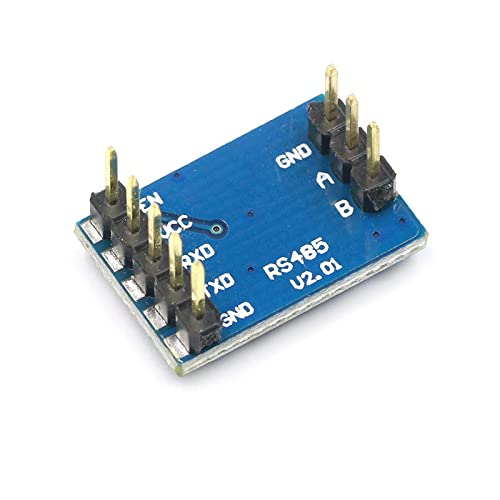
\includegraphics[width=\textwidth]{composants/MAX3485_avec_broche_EN.jpg}
        \caption{RS-485 transceiver module.}
        \label{fig:comp_rs485}
    \end{subfigure}
    \hfill
    \begin{subfigure}[b]{0.25\textwidth}
        \centering
        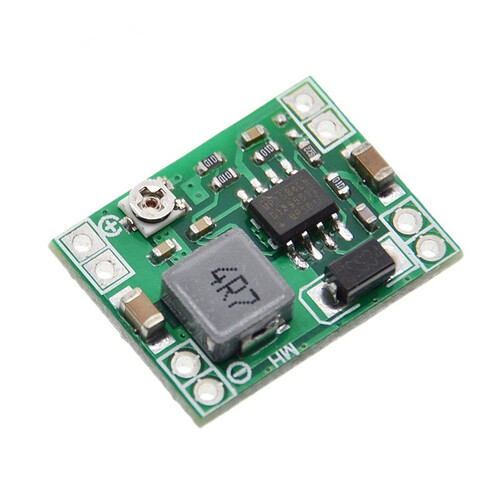
\includegraphics[width=\textwidth]{composants/DCDC_converter.jpeg}
        \caption{DC-DC converter (MP2307).}
        \label{fig:comp_buck}
    \end{subfigure}
    \caption{Components of the new \textit{main board}.}
    \label{fig:composants}
\end{figure}

Resolving this bottleneck required replacing the \textit{Atomic RS485} base with a custom hardware solution where the DE direction pin is explicitly driven by the microcontroller. To implement this, the two new components shown in Figure~\ref{fig:composants} were acquired. First, the architecture relies on a 3.3\,V RS-485 transceiver board with an exposed DE pin (MAX3485-type~\cite{max3485}). Furthermore, because the original base internally handled power regulation, this modification required adding a dedicated 12–16\,V to 5\,V step-down converter, implemented here with a compact MP2307 module~\cite{mp2307}.

On the software side, the PlatformIO bus driver was updated to leverage the hardware RS-485 half-duplex mode of the ESP32-S3's UART~\cite{esp32s3_uart}. By linking the transceiver's DE pin to the UART controller's RTS pin, the transmit/receive direction is toggled automatically in direct synchronization with the last transmitted stop bit, which allows to eliminate software latency and frees the bus in under a microsecond, reliably supporting baud rates of 1 Mbps and up to 3 Mbps. This explicit direction control allows the motors' \textit{Return Delay Time} to be minimized, securing the high-frequency control loop and laying the groundwork for the final main board architecture.


\subsection{New Main Board and Configuration}

When the components arrived, I assembled the new control board with the three active elements showing in the figure~\ref{fig:composants}, the AtomS3R microcontroller~\cite{m5stack_atoms3r}, the RS-485 transceiver module with an accessible direction pin, and the DC-DC step-down converter supplying the logic power.

\newpage

Above all, this new architecture made it possible, for the first time, to test the \emph{real} motors of the robot. In fact, the SWUMANOID is driven by three families of XW-series Dynamixel servomotors (waterproof, IP68 rating), spread across the body according to their torque needs presented in the figure~\ref{fig:swumanoid_map}: XW540-T140-R and XW540-T260-R~\cite{dynamixel_xw540t140,dynamixel_xw540t260} for the most heavily loaded joints, and XW430-T200-R~\cite{dynamixel_xw430t200} for the distal joints, all these motors are waterproof.

\begin{figure}[H]
    \centering
    \begin{subfigure}[b]{0.34\textwidth}
        \centering
        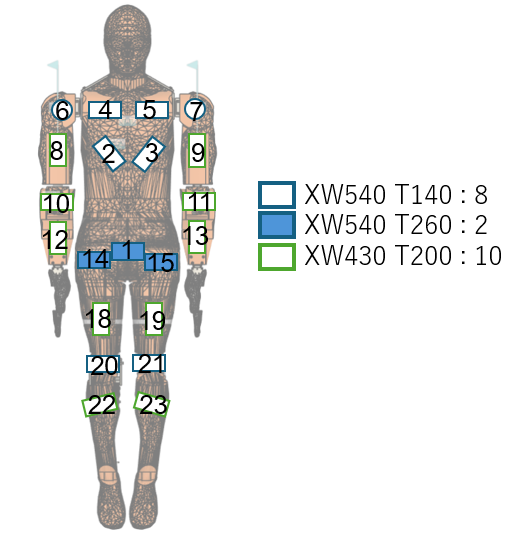
\includegraphics[height=6cm]{schemas/swumanoid_motor_map.png}
        \caption{Motor layout on the SWUMANOID.}
        \label{fig:map_body}
    \end{subfigure}
    \hfill
    \begin{subfigure}[b]{0.24\textwidth}
        \centering
        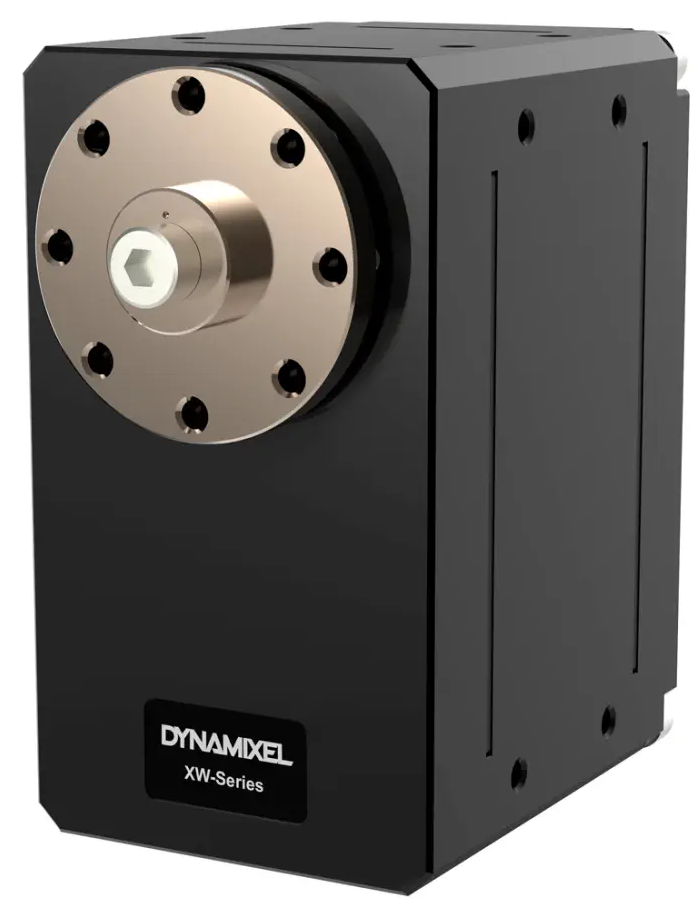
\includegraphics[height=5cm]{composants/XW_series_motors_dynamixel.png}
        \caption{XW-series Dynamixel.}
        \label{fig:motor_xw}
    \end{subfigure}
    \hfill
    \begin{subfigure}[b]{0.24\textwidth}
        \centering
        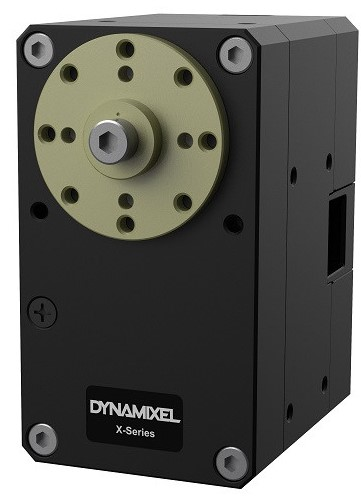
\includegraphics[height=5cm]{composants/xm540-w150.jpg}
        \caption{XM-series Dynamixel.}
        \label{fig:motor_xm}
    \end{subfigure}
    \caption{SWUMANOID motor configuration.}
    \label{fig:swumanoid_map}
\end{figure}

So, to validate the hardware architecture under representative conditions, I built a test circuit combining the new components with a cluster of five \emph{real} Dynamixel motors from the robot with two XW430-T200-R, two XW540-T260-R and one XW540-T140-R. Each was given the ID matching its actual function in the SWUMANOID, so the bench faithfully reproduces a subset of the robot rather than an arbitrary assembly. The XW540-T140-R thus corresponds to a \textbf{shoulder joint}, whose behavior gets a detailed analysis in the results section. Unlike the first bench, limited to substitute motors, this configuration uses far more powerful and extremely responsive, they allow much better command tracking.

\begin{figure}[H]
    \centering
    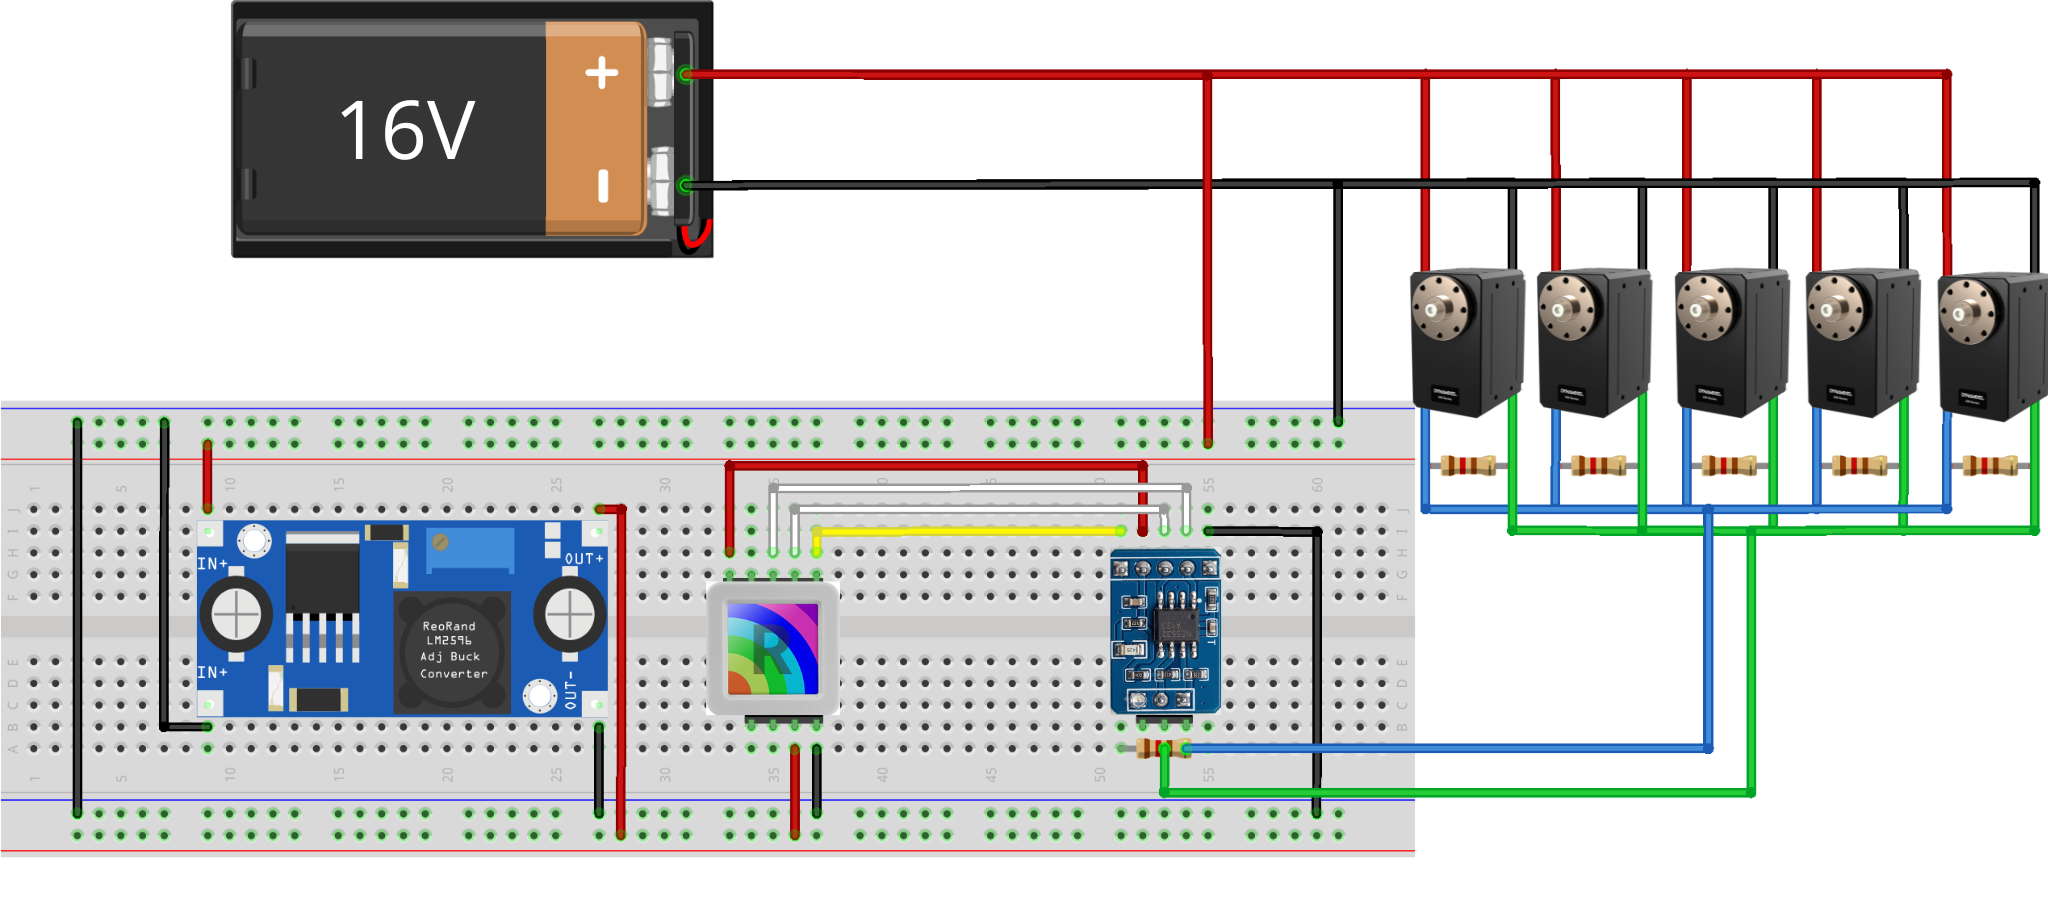
\includegraphics[width=0.9\textwidth]{schemas/schema_5_moteurs_haut_baudrate.png}
    \caption{New control circuit tested on the five XW motors.}
    \label{fig:circuit_test}
\end{figure}

To make this new circuit safe, the power architecture was split into a power stage and a logic stage. A 16\,V power line, straight from the generator, supplies the Dynamixel motors, it is also fed into the DC-DC step-down converter, a compact module recognizable by its inductor marked "4R7", based on the MP2307~\cite{mp2307}, which turns it into a stable 5\,V for the AtomS3R. The logic stage of the MAX3485 module is powered at 3.3\,V directly from the AtomS3R, to keep the signal levels perfectly aligned. Finally, all the grounds (GND) of the generator, the converter, the AtomS3R and the MAX3485 were tied together for a strict common ground, with no reference drift. Within this circuit showed in the figure~\ref{fig:circuit_test}, the ESP32-S3 architecture allows flexible pin routing. I configured the communication lines as follows, in line with the embedded bus driver:
\begin{itemize}
    \item the \textbf{DI} pin (\textit{Driver Input}, data to transmit) of the MAX3485 is connected to the microcontroller's \textbf{TX} output, on GPIO \textbf{G6}.
    \item the \textbf{RO} pin (\textit{Receiver Output}, received data) is connected to the \textbf{RX} input, on GPIO \textbf{G5}.
    \item the \textbf{DE/RE} direction pins (\textit{Enable}) are tied together and driven by a free GPIO (\textbf{G7}), wired to the UART's RTS pin for automatic hardware switching.
\end{itemize}

Finally, to keep the signal clean at high speed and absorb reflections, the RS-485 bus was secured, as on the first bench, with two 120\,$\Omega$ termination resistors. This board finally comes with the software change anticipated above. In the \texttt{drivers/motor\_bus} driver, opening the hardware UART is now completed by enabling the ESP32-S3's RS-485 half-duplex mode~\cite{esp32s3_uart}, tying the RTS pin (here G7) to the transceiver's DE/RE direction. The bus throughput, set centrally in \texttt{firmware\_config.h}, is raised from 3\,Mbps toward the high-speed target, and each motor's \textit{Return Delay Time} is reduced accordingly. For the protocol layer, Dynamixel~2.0 frames, CRC-16, \texttt{SyncWrite}/\texttt{SyncRead}, already validated on the first bench, it stays unchanged.

So the five-motor bench proved the electronics were sound but it was still a loose prototype, modules held together by jumper wires whixh is a problem. On a desk it works fine but inside the robot it does not because the MP2307 converter turned out to be simply too tall for the small waterproof box that lives in the SWUMANOID's head, and it would not go in no matter how I placed it.

So I ordered two smaller parts shown in the figure~\ref{fig:new_components}. The first is a MINMAX M78AR05 step-down module, a tiny drop-in replacement for the bulky MP2307 that still delivers the same clean 5\,V rail~\cite{minmax_m78ar05}. The second is a compact soldering PCB, small enough to rest on the floor of the inner case.

\begin{figure}[H]
    \centering
    \begin{subfigure}[b]{0.4\textwidth}
        \centering
        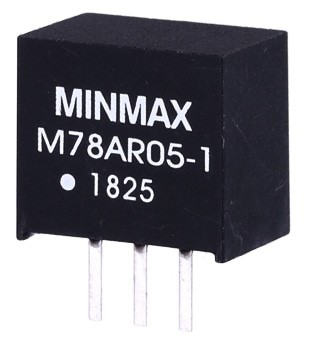
\includegraphics[height=4cm]{composants/DCDC_converter_MINMAX.jpg}
        \caption{MINMAX M78AR05 step-down converter.}
        \label{fig:comp_minmax}
    \end{subfigure}
    \hfill
    \begin{subfigure}[b]{0.4\textwidth}
        \centering
        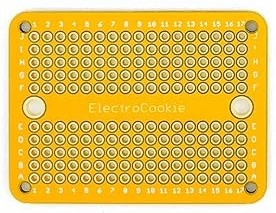
\includegraphics[height=4cm]{composants/PCB_Board.jpg}
        \caption{Compact soldering PCB (ElectroCookie).}
        \label{fig:comp_pcb}
    \end{subfigure}
    \caption{The two smaller parts chosen to shrink the board down to size.}
    \label{fig:new_components}
\end{figure}

Then, we moved the whole circuit off the breadboard and onto that PCB. The AtomS3R, the MAX3485, the little converter and the termination resistors were all soldered down and wired point to point, so nothing can pop loose when the lid is closed and the board came out small, flat and sturdy. It drops straight into the waterproof case, which in turn slots into the head we can see in figure~\ref{fig:final_board}.

\begin{figure}[H]
    \centering
    \begin{subfigure}[b]{0.38\textwidth}
        \centering
        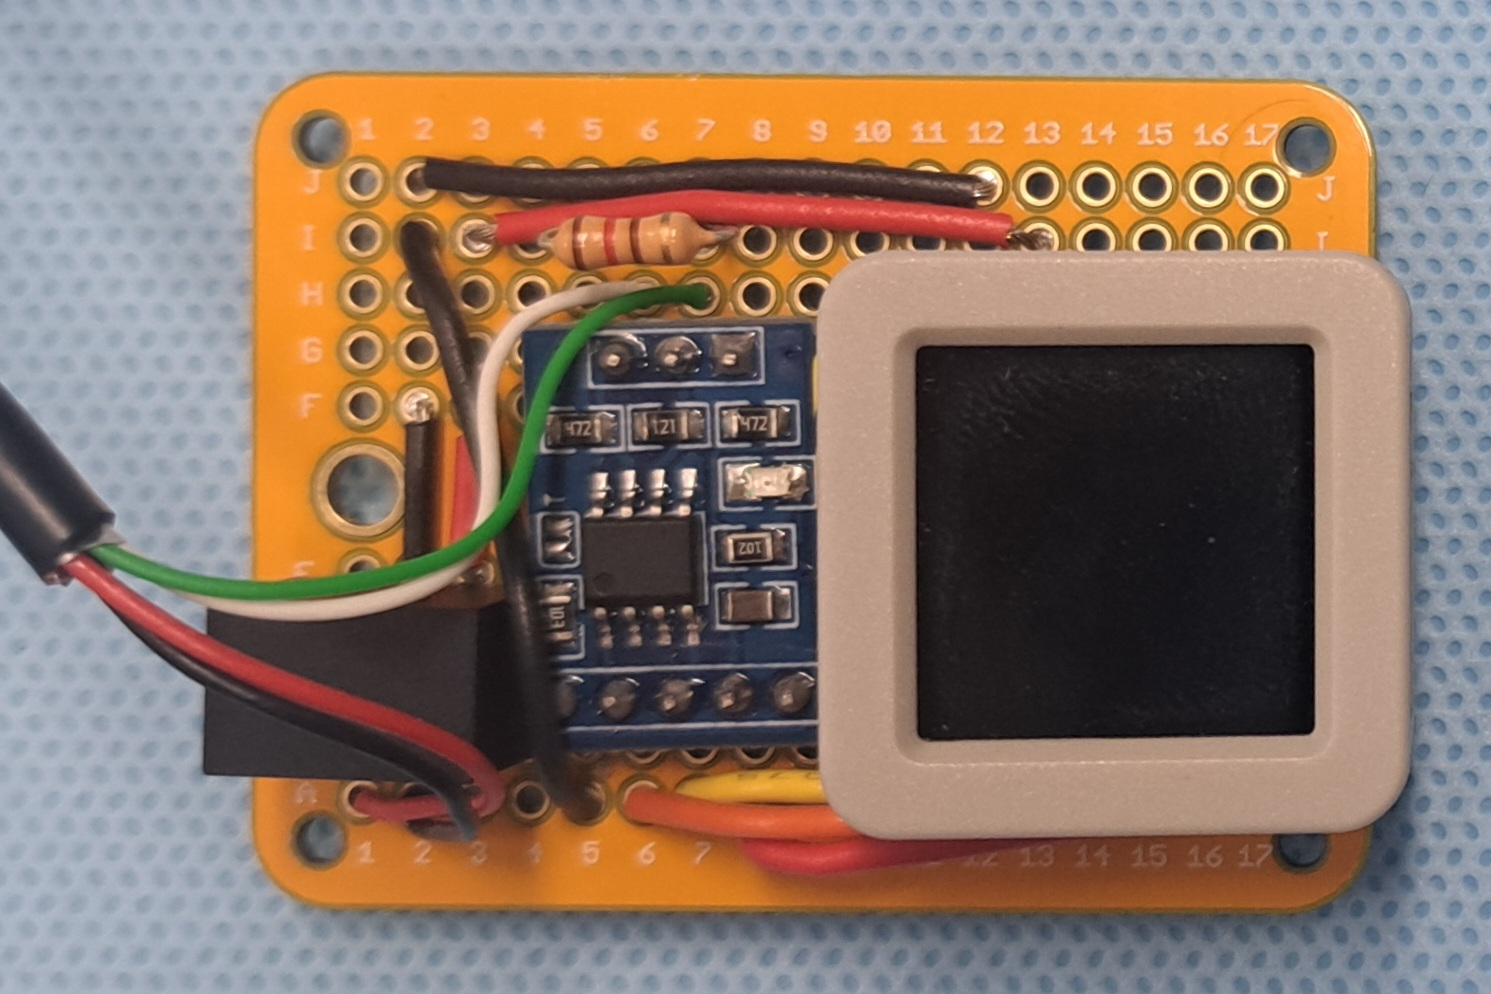
\includegraphics[width=\textwidth]{composants/New_Main_Board.jpg}
        \caption{The soldered main board.}
        \label{fig:board_soldered}
    \end{subfigure}
    \hfill
    \begin{subfigure}[b]{0.23\textwidth}
        \centering
        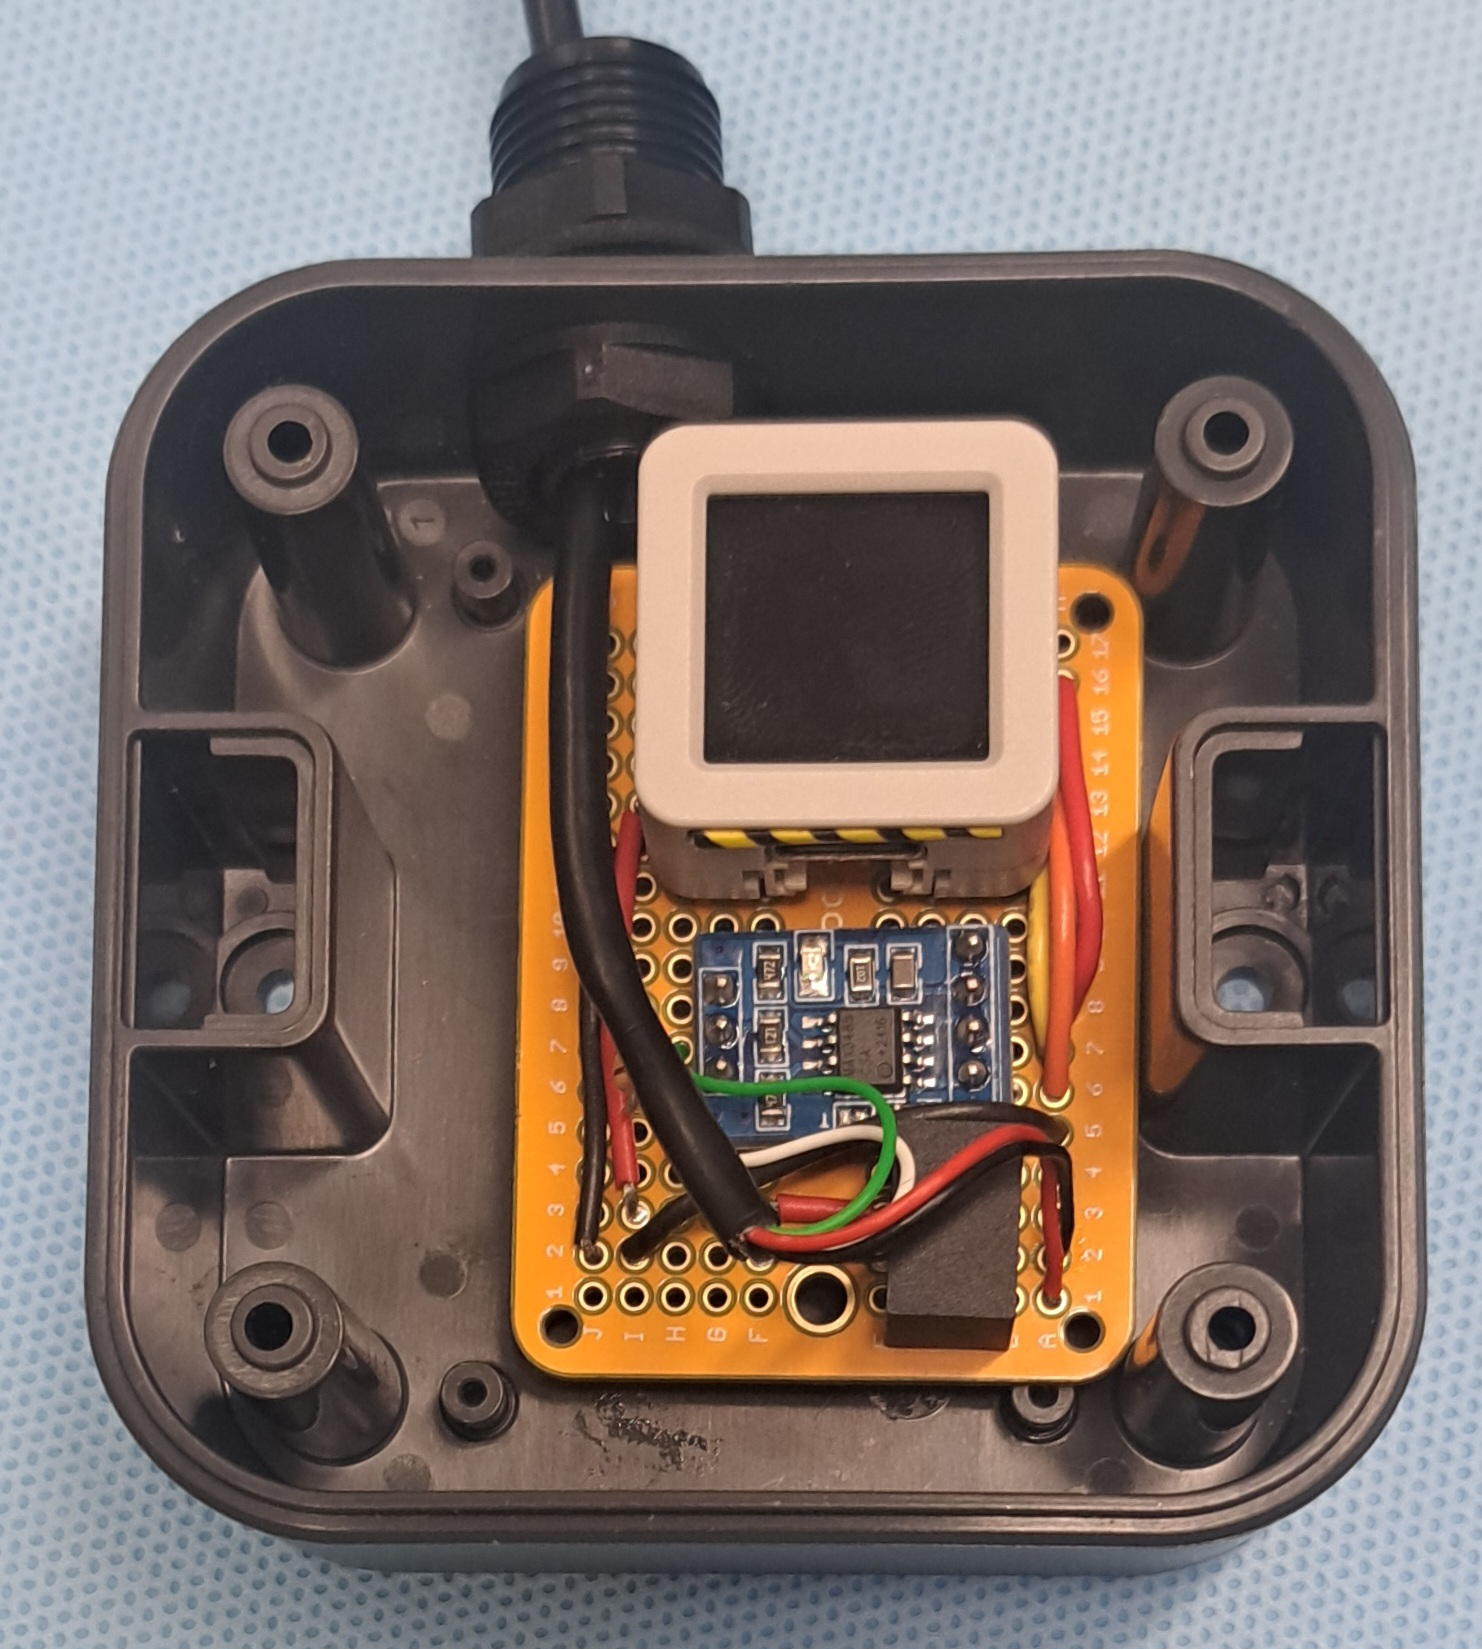
\includegraphics[width=\textwidth]{composants/New_Main_Board_in_case.jpg}
        \caption{Mounted in the waterproof case.}
        \label{fig:board_case}
    \end{subfigure}
    \hfill
    \begin{subfigure}[b]{0.31\textwidth}
        \centering
        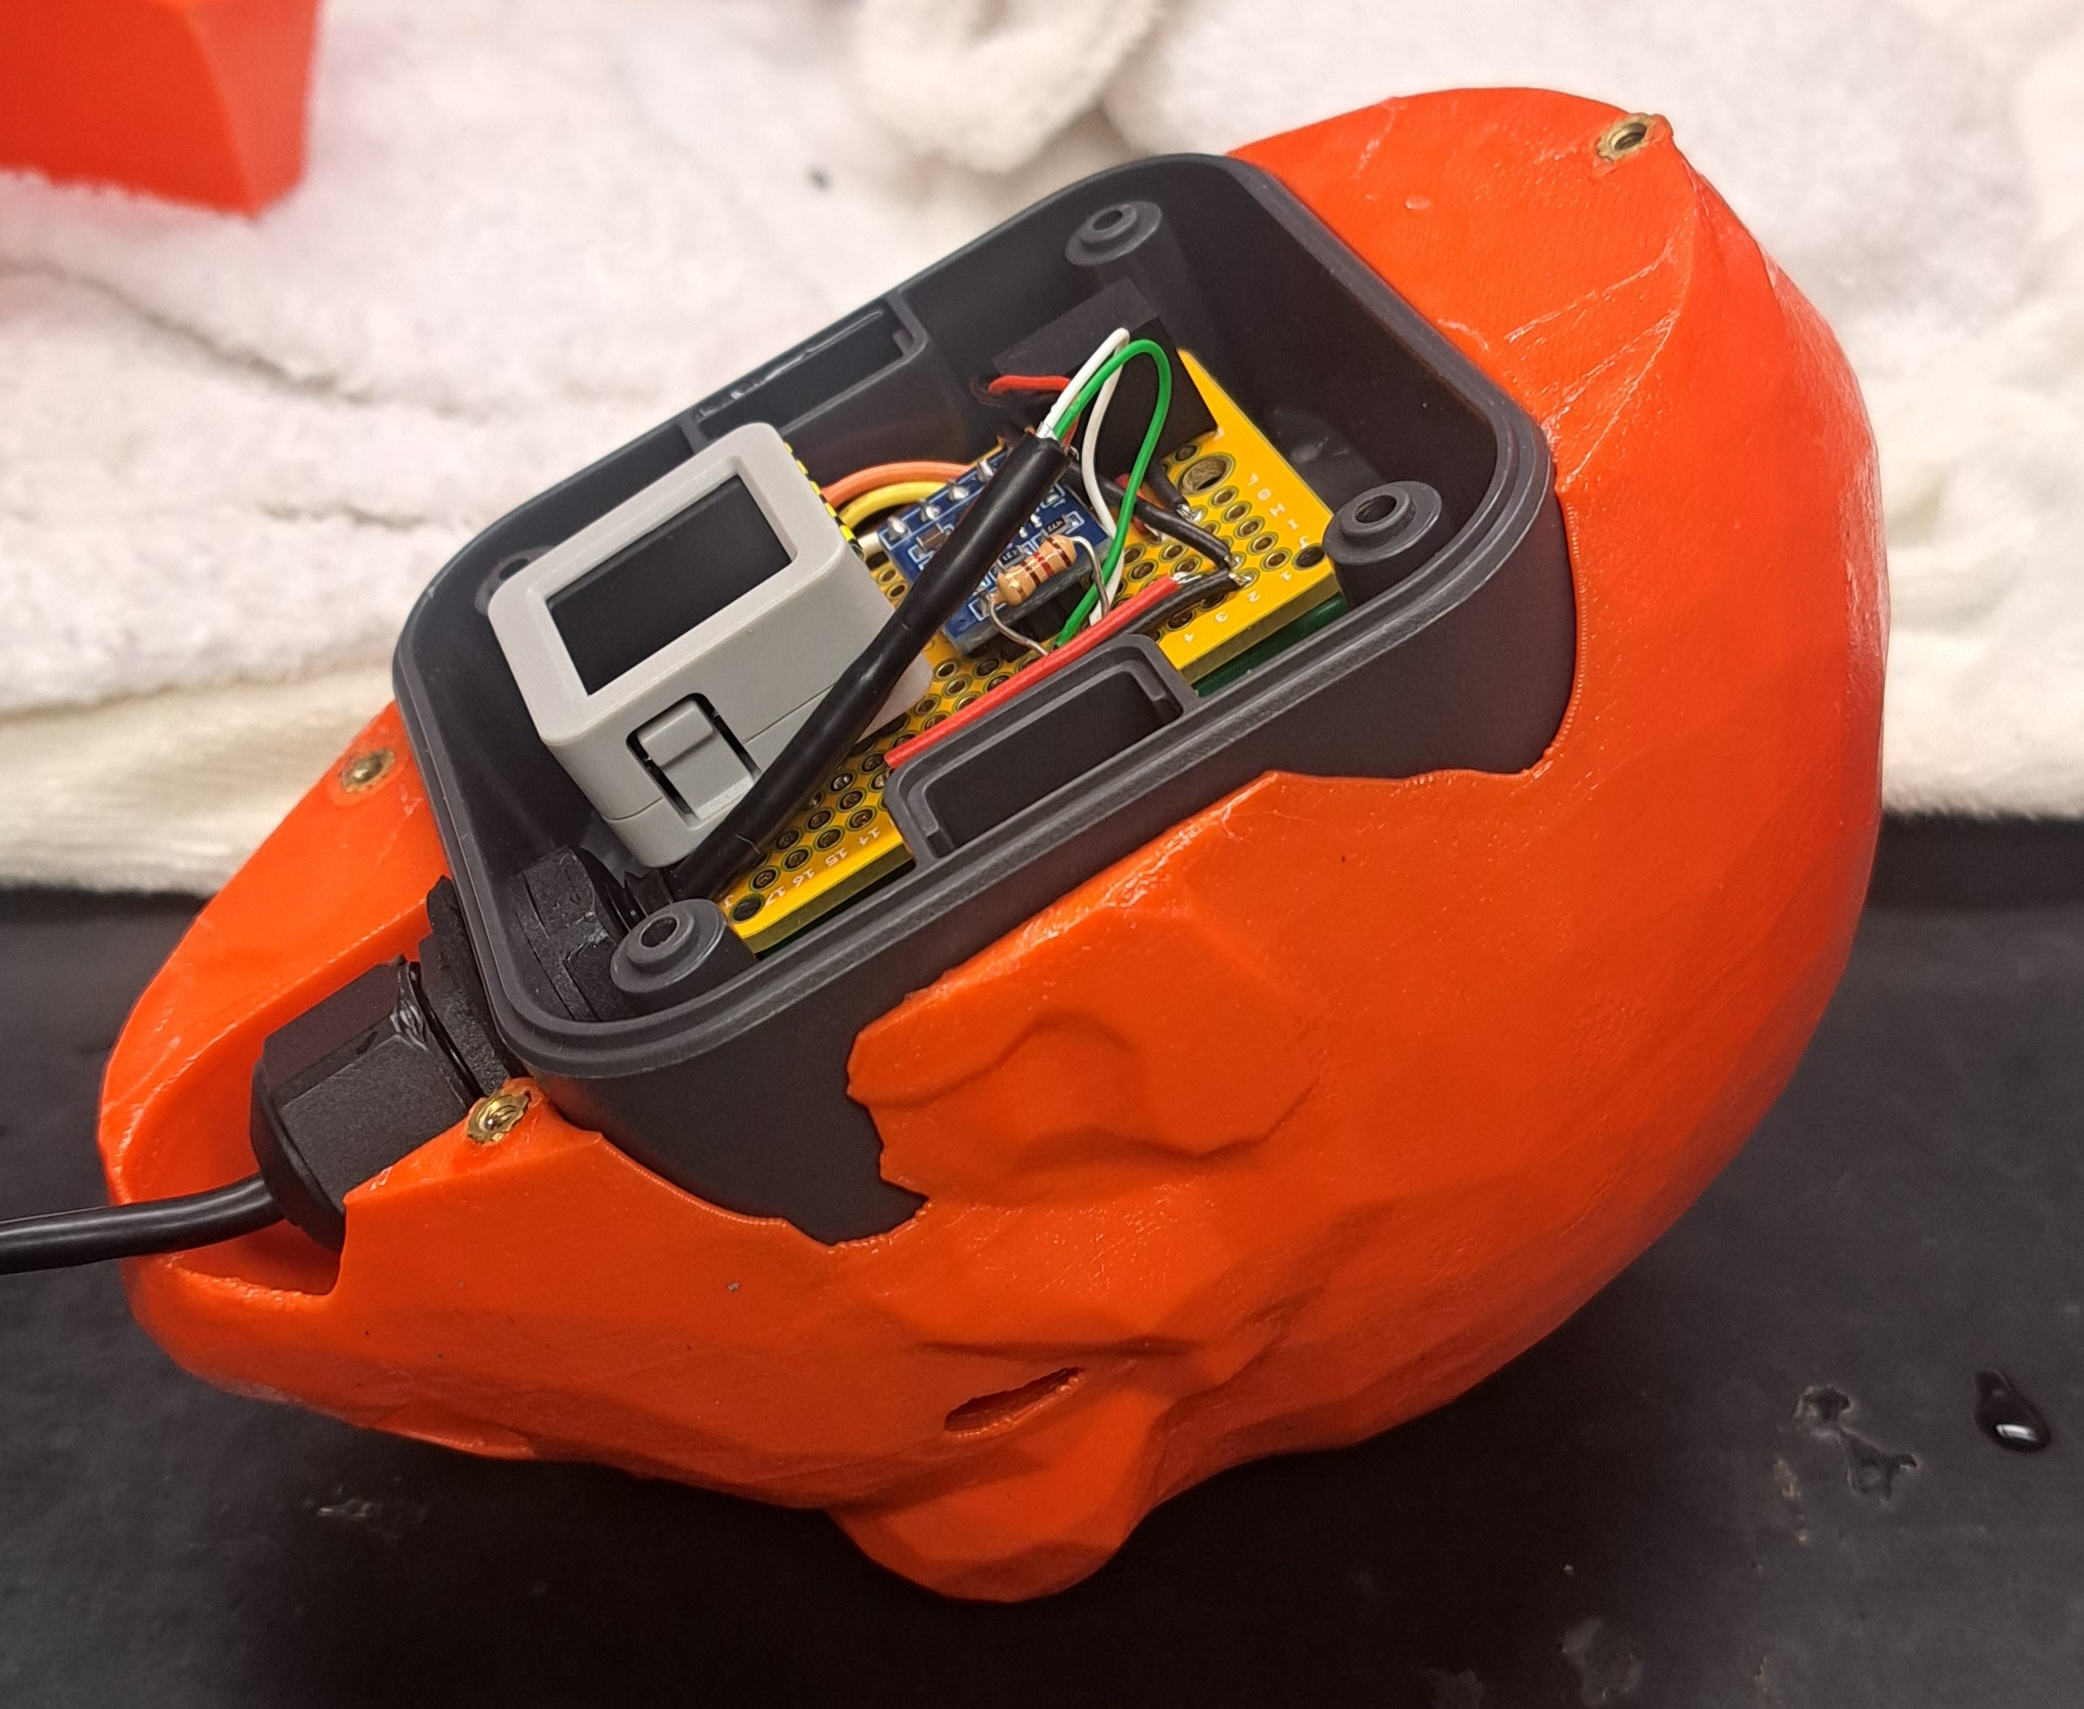
\includegraphics[width=\textwidth]{composants/New_Main_Board_in_head.jpg}
        \caption{Installed in the robot's head.}
        \label{fig:board_head}
    \end{subfigure}
    \caption{The final soldered main board and its integration into the SWUMANOID's head.}
    \label{fig:final_board}
\end{figure}

This represents the final state of the controller as a single soldered board securely housed inside the robot, driving all twenty-one motors at high frequency. All subsequent pool experiments rely on this hardware and working good.

\subsection{Results at High Baud Rate}

With this new assembly, taking back control of the EN pin, the transmit/receive switch happens with no latency at all. I was able to raise the baud rate to \textbf{3 Mbps} with perfect motor detection and zero packet loss. Freeing up this bandwidth reduces the bus occupancy time, so the cost of polling one motor, which reached 3 to 4\,ms on the slow, auto-direction bus (previous section), collapses here to the hundred-microsecond scale. This reduction, combined with the lower \textit{Return Delay Time} now allowed by explicit direction control, is what finally makes a high-frequency control loop reachable.

\begin{figure}[H]
    \centering
    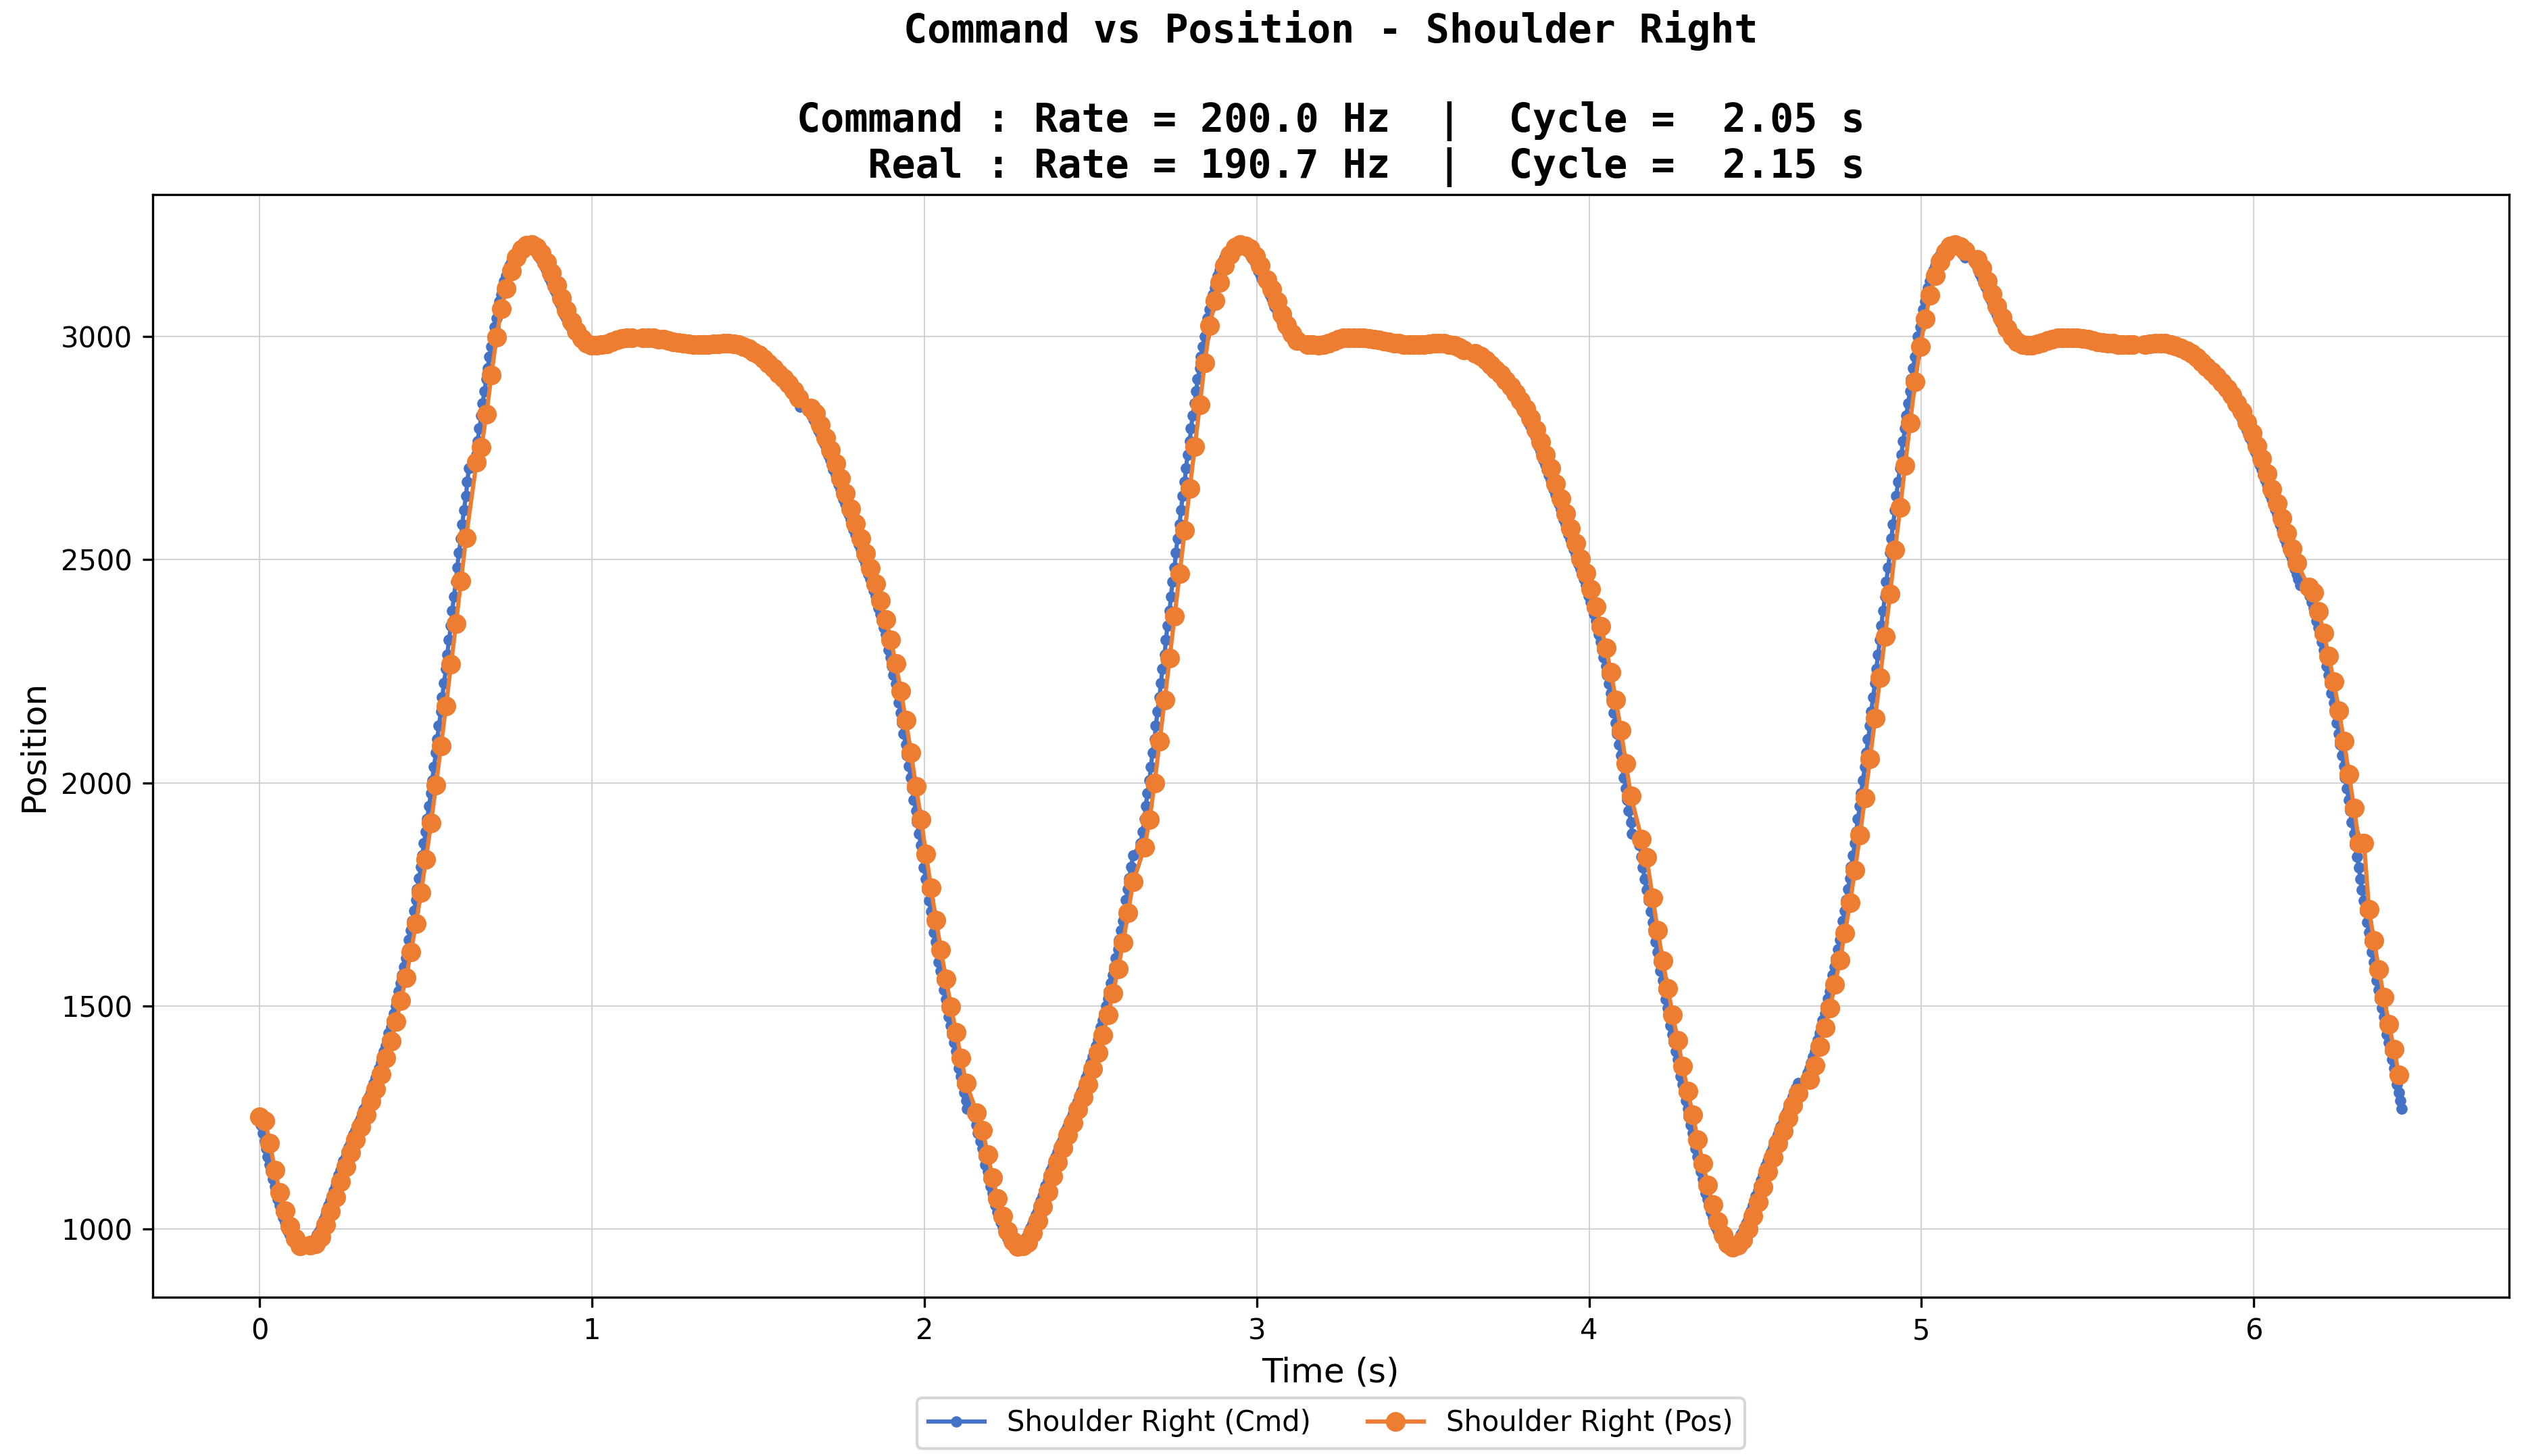
\includegraphics[width=0.7\textwidth]{graphiques/202607241639_ID_4_200Hz.png}
    \caption{Comparison of the command and the actual position of the right shoulder (200\,Hz).}
    \label{fig:graph_200hz}
\end{figure}

As the figure \ref{fig:graph_200hz} shows, the running system behaves excellently. We reach a real frequency of \textbf{190.7 Hz} for a 200.0 Hz setpoint. Above all, unlike the old iterations where trajectory tracking was catastrophic, the measured positions (in orange) now sit perfectly on top of the command sent (in blue). The robot finally has an ultra-responsive control loop, which is essential for the next developments on the swimming dynamics.

With tracking validated, it remained to quantify the price of telemetry on the loop rate and as established earlier, reading states with \texttt{SyncRead} is sequential on a \textit{half-duplex} bus, in fact, after a single broadcast instruction, the polled motors answer one after another~\cite{dynamixel_x_manual}. The bus occupancy per read therefore grows with the number of logged motors $N$. So to isolate this factor, I ran a campaign where \emph{all} the selected motors are polled \emph{every $K = 3$ frames} (a single \texttt{SyncRead} pass per read), varying only their number $N$, from 1 to 5, with the setpoint held at 200\,Hz.

\iffalse
\begin{figure}[H]
    \centering
    \begin{subfigure}[b]{0.49\textwidth}
        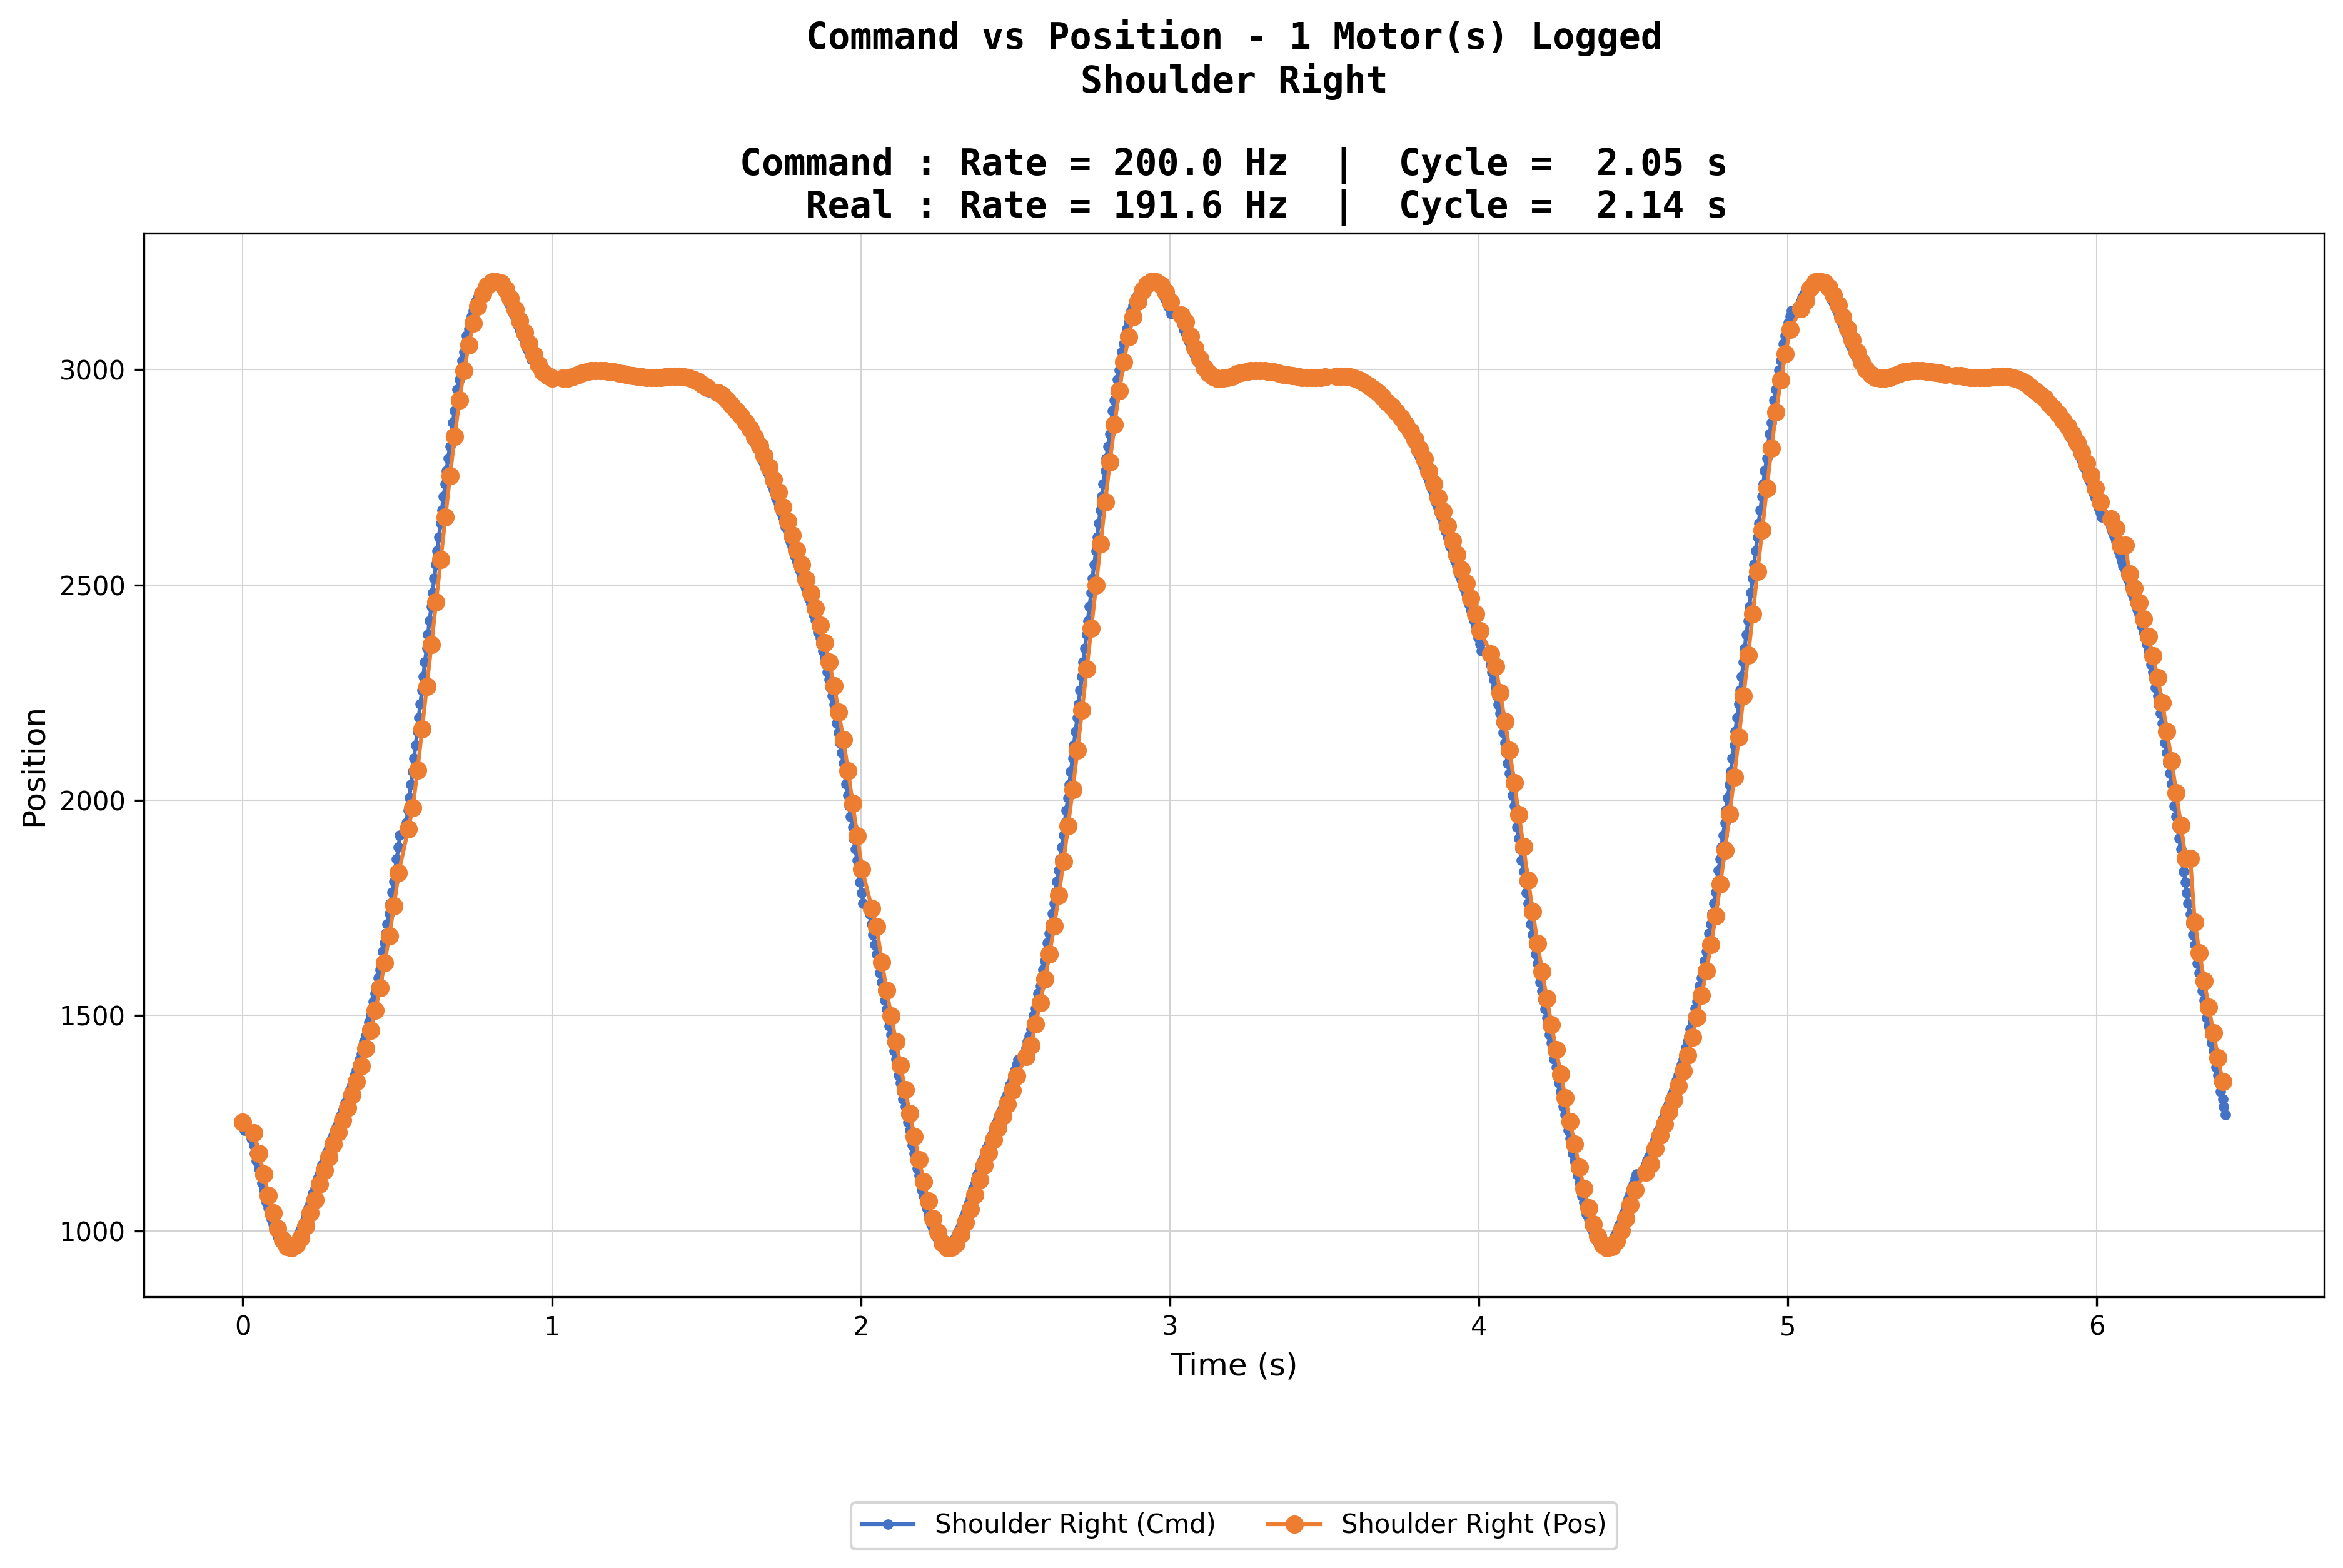
\includegraphics[width=\textwidth]{graphiques/log_1mot_200Hz.png}
        \caption{$N = 1$ motor $\rightarrow$ 191.6 Hz.}
        \label{fig:ssweep1}
    \end{subfigure}
    \hfill
    \begin{subfigure}[b]{0.49\textwidth}
        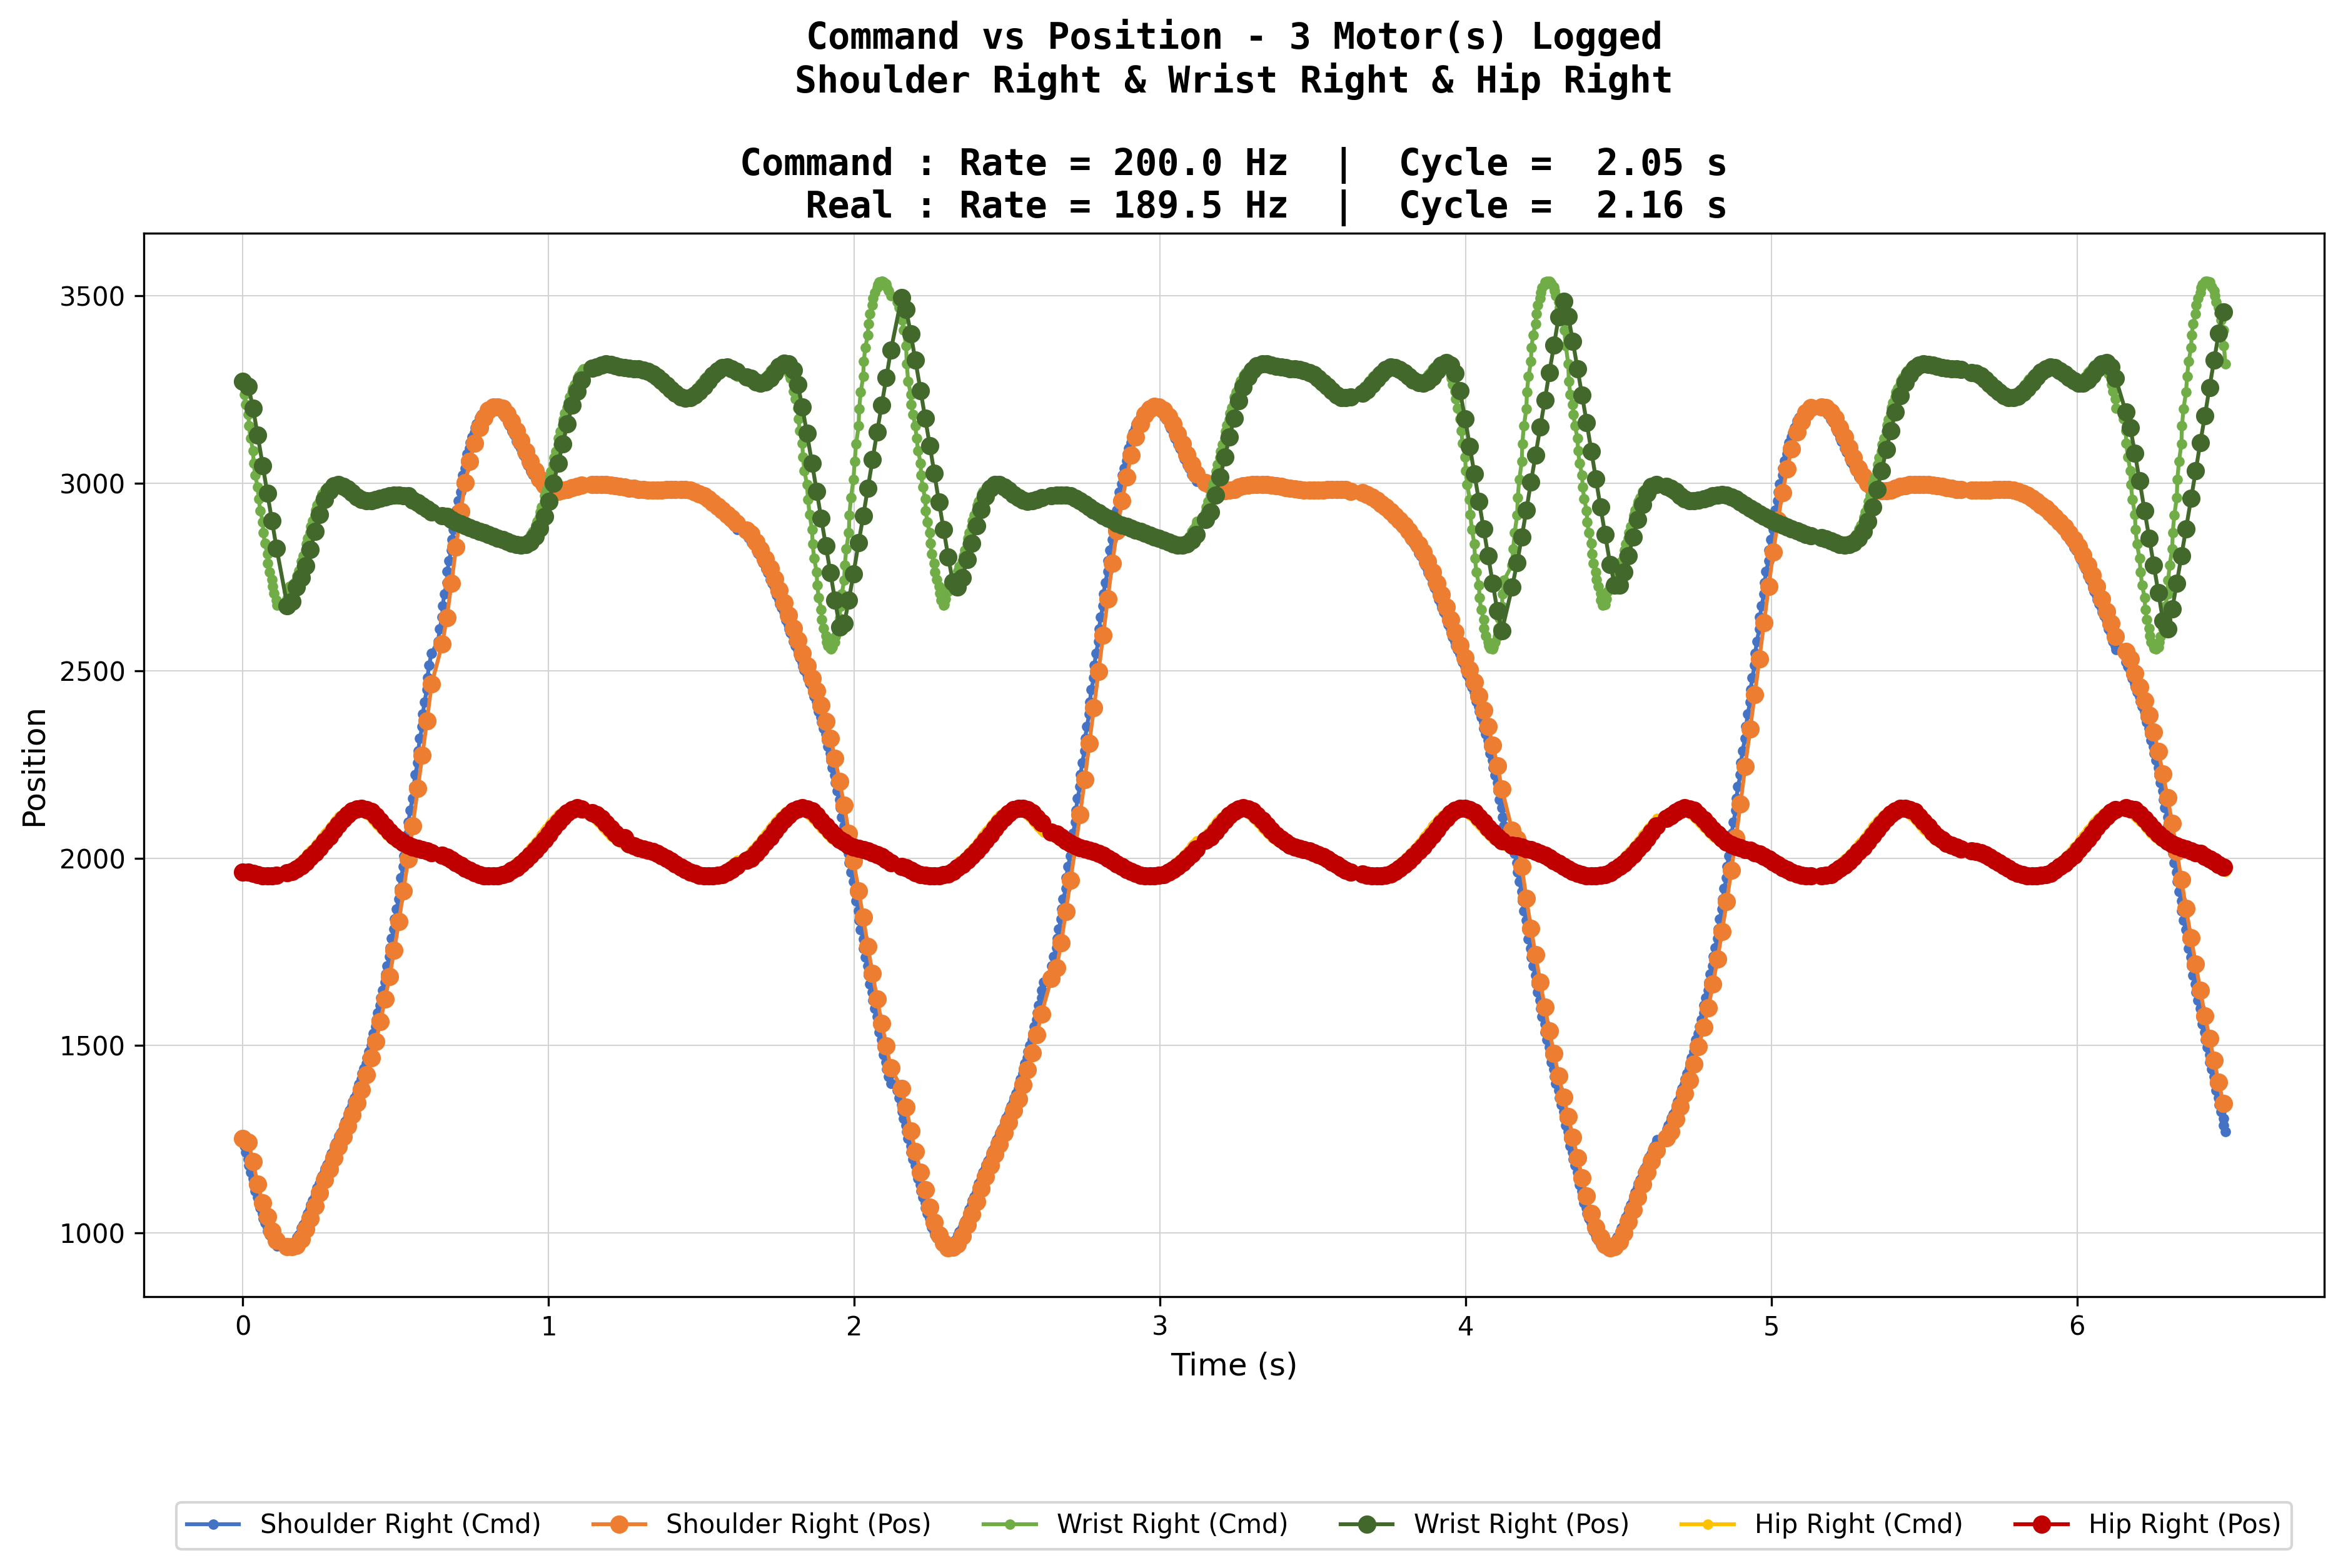
\includegraphics[width=\textwidth]{graphiques/log_3mot_200Hz.png}
        \caption{$N = 3$ motors $\rightarrow$ 189.5 Hz.}
        \label{fig:ssweep3}
    \end{subfigure}
    \caption{Effect of the number of logged motors $N$ on control frequency for 1 and 3 motors (200\,Hz and $K = 3$ frames).}
    \label{fig:sweep_motors_part1}
\end{figure}

\begin{figure}[H]
    \centering
    \begin{subfigure}[b]{0.49\textwidth}
        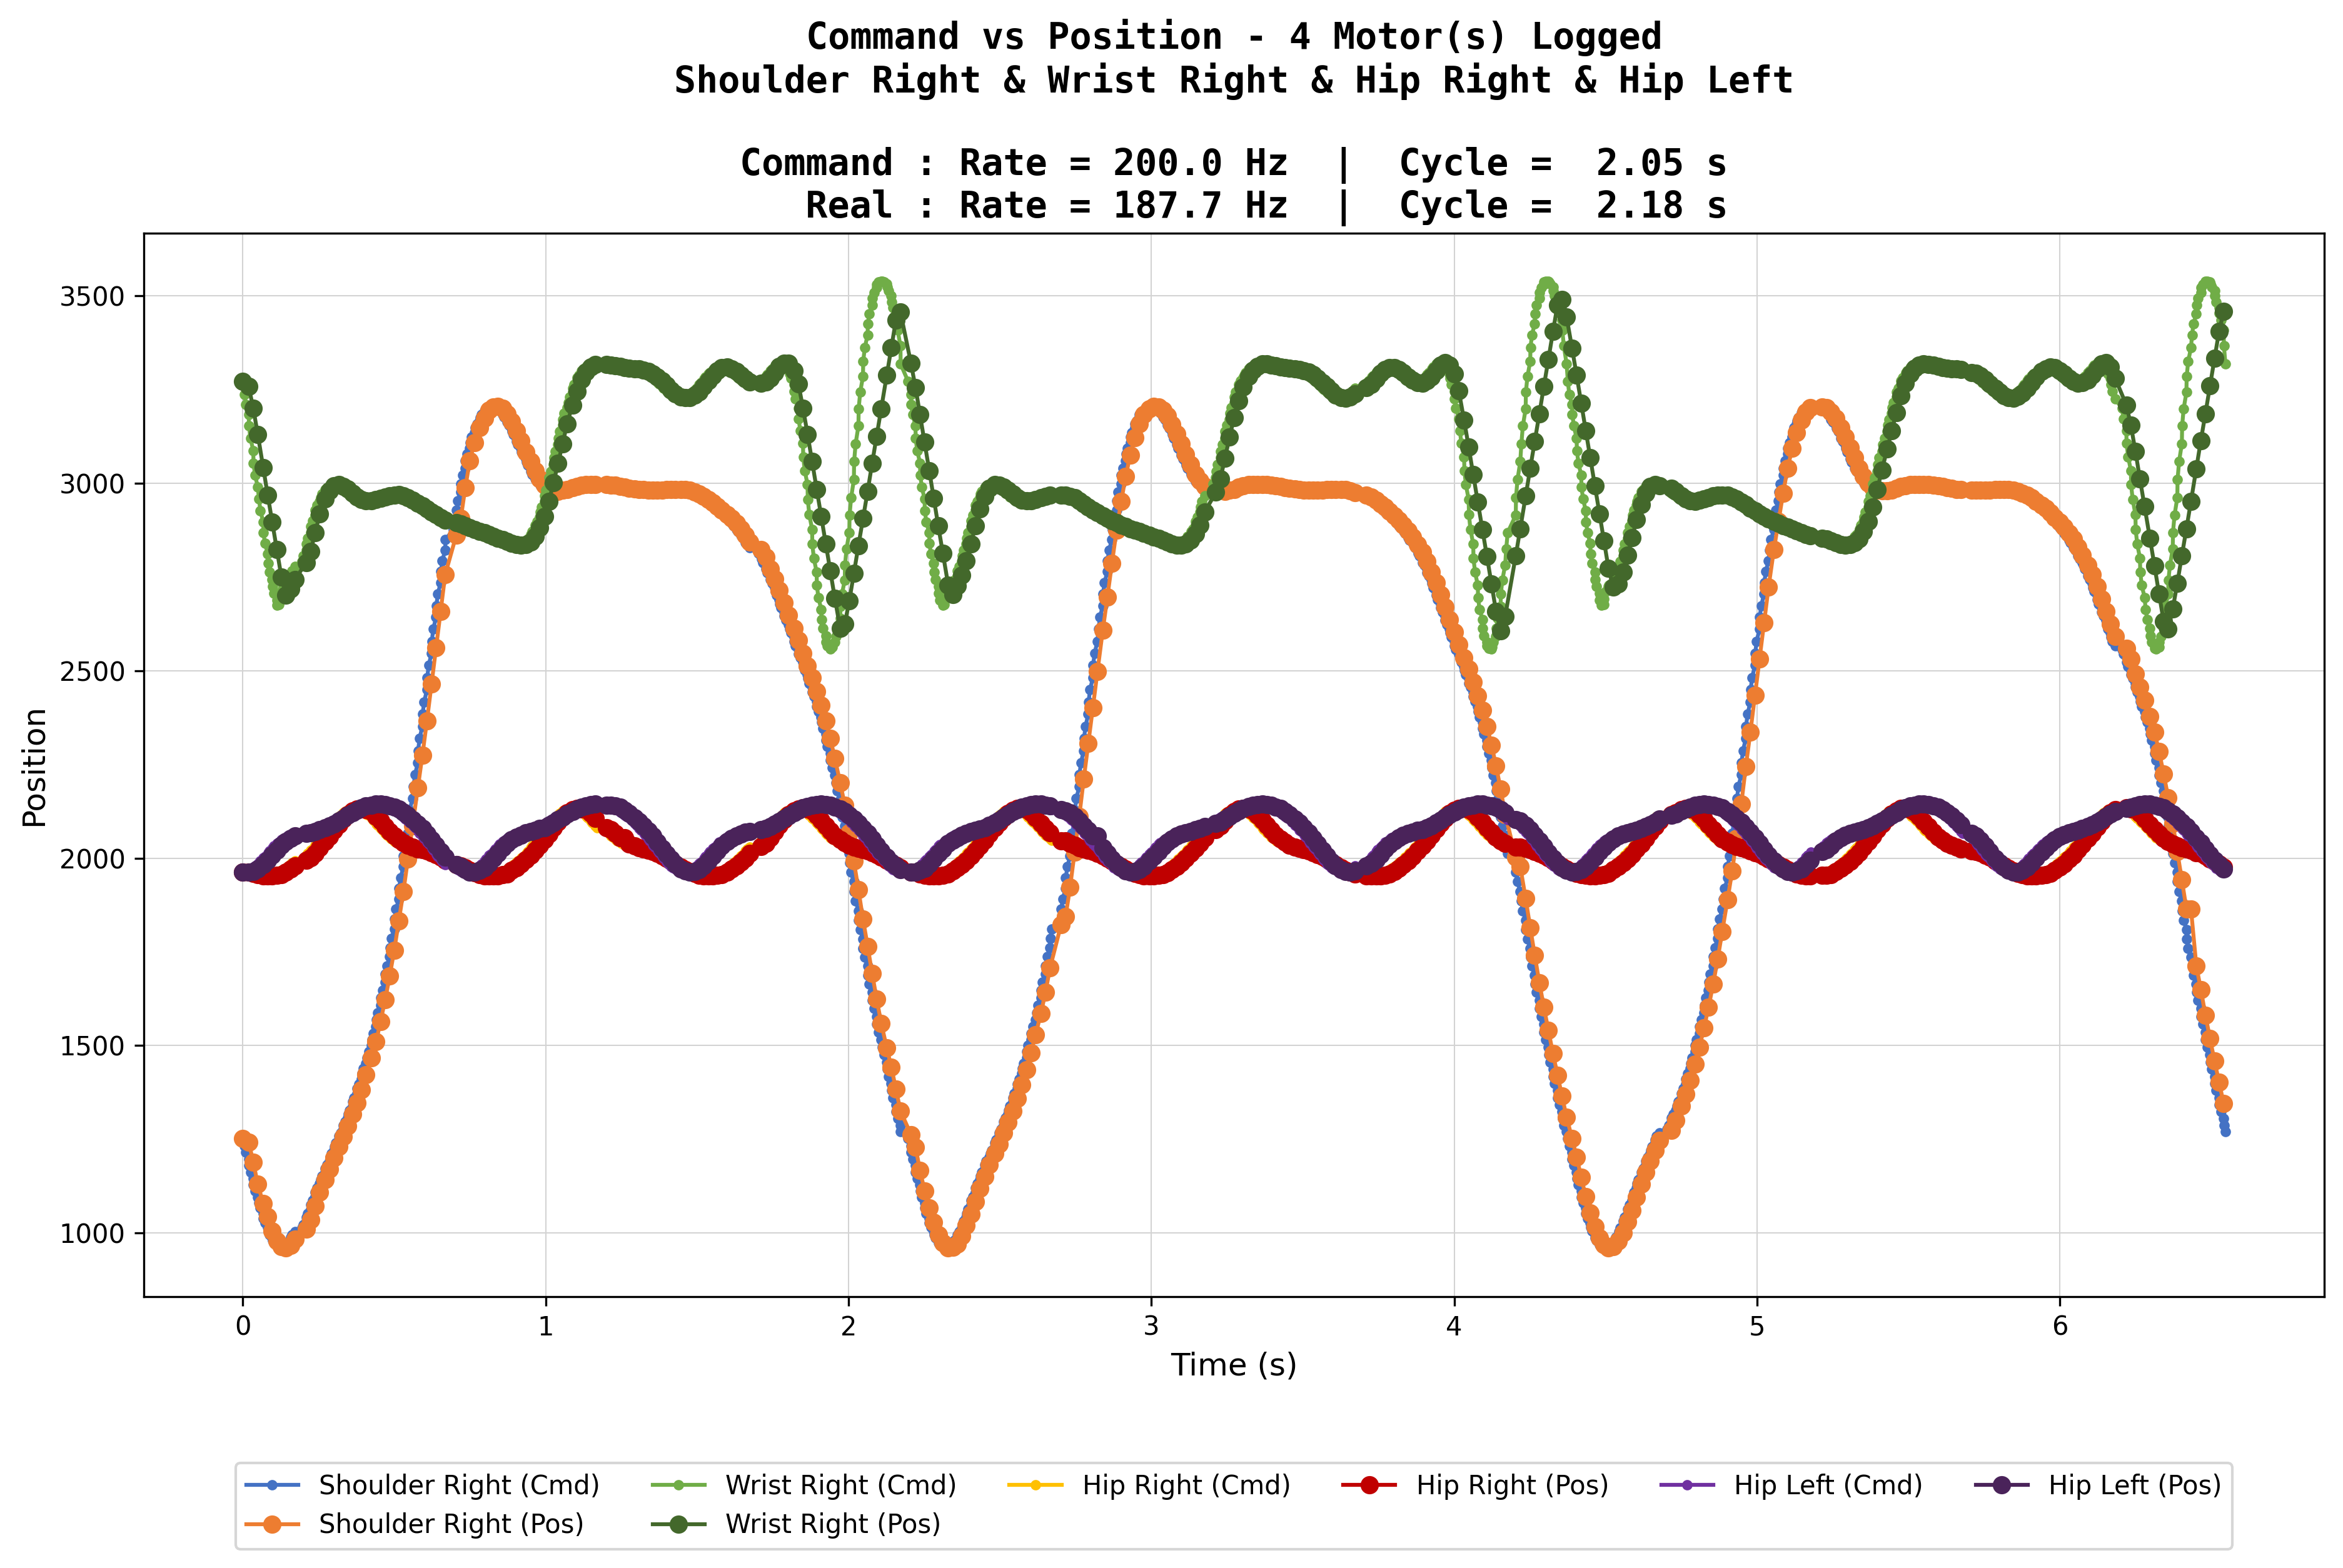
\includegraphics[width=\textwidth]{graphiques/log_4mot_200Hz.png}
        \caption{$N = 4$ motors $\rightarrow$ 187.7 Hz.}
        \label{fig:ssweep4}
    \end{subfigure}
    \hfill
    \begin{subfigure}[b]{0.49\textwidth}
        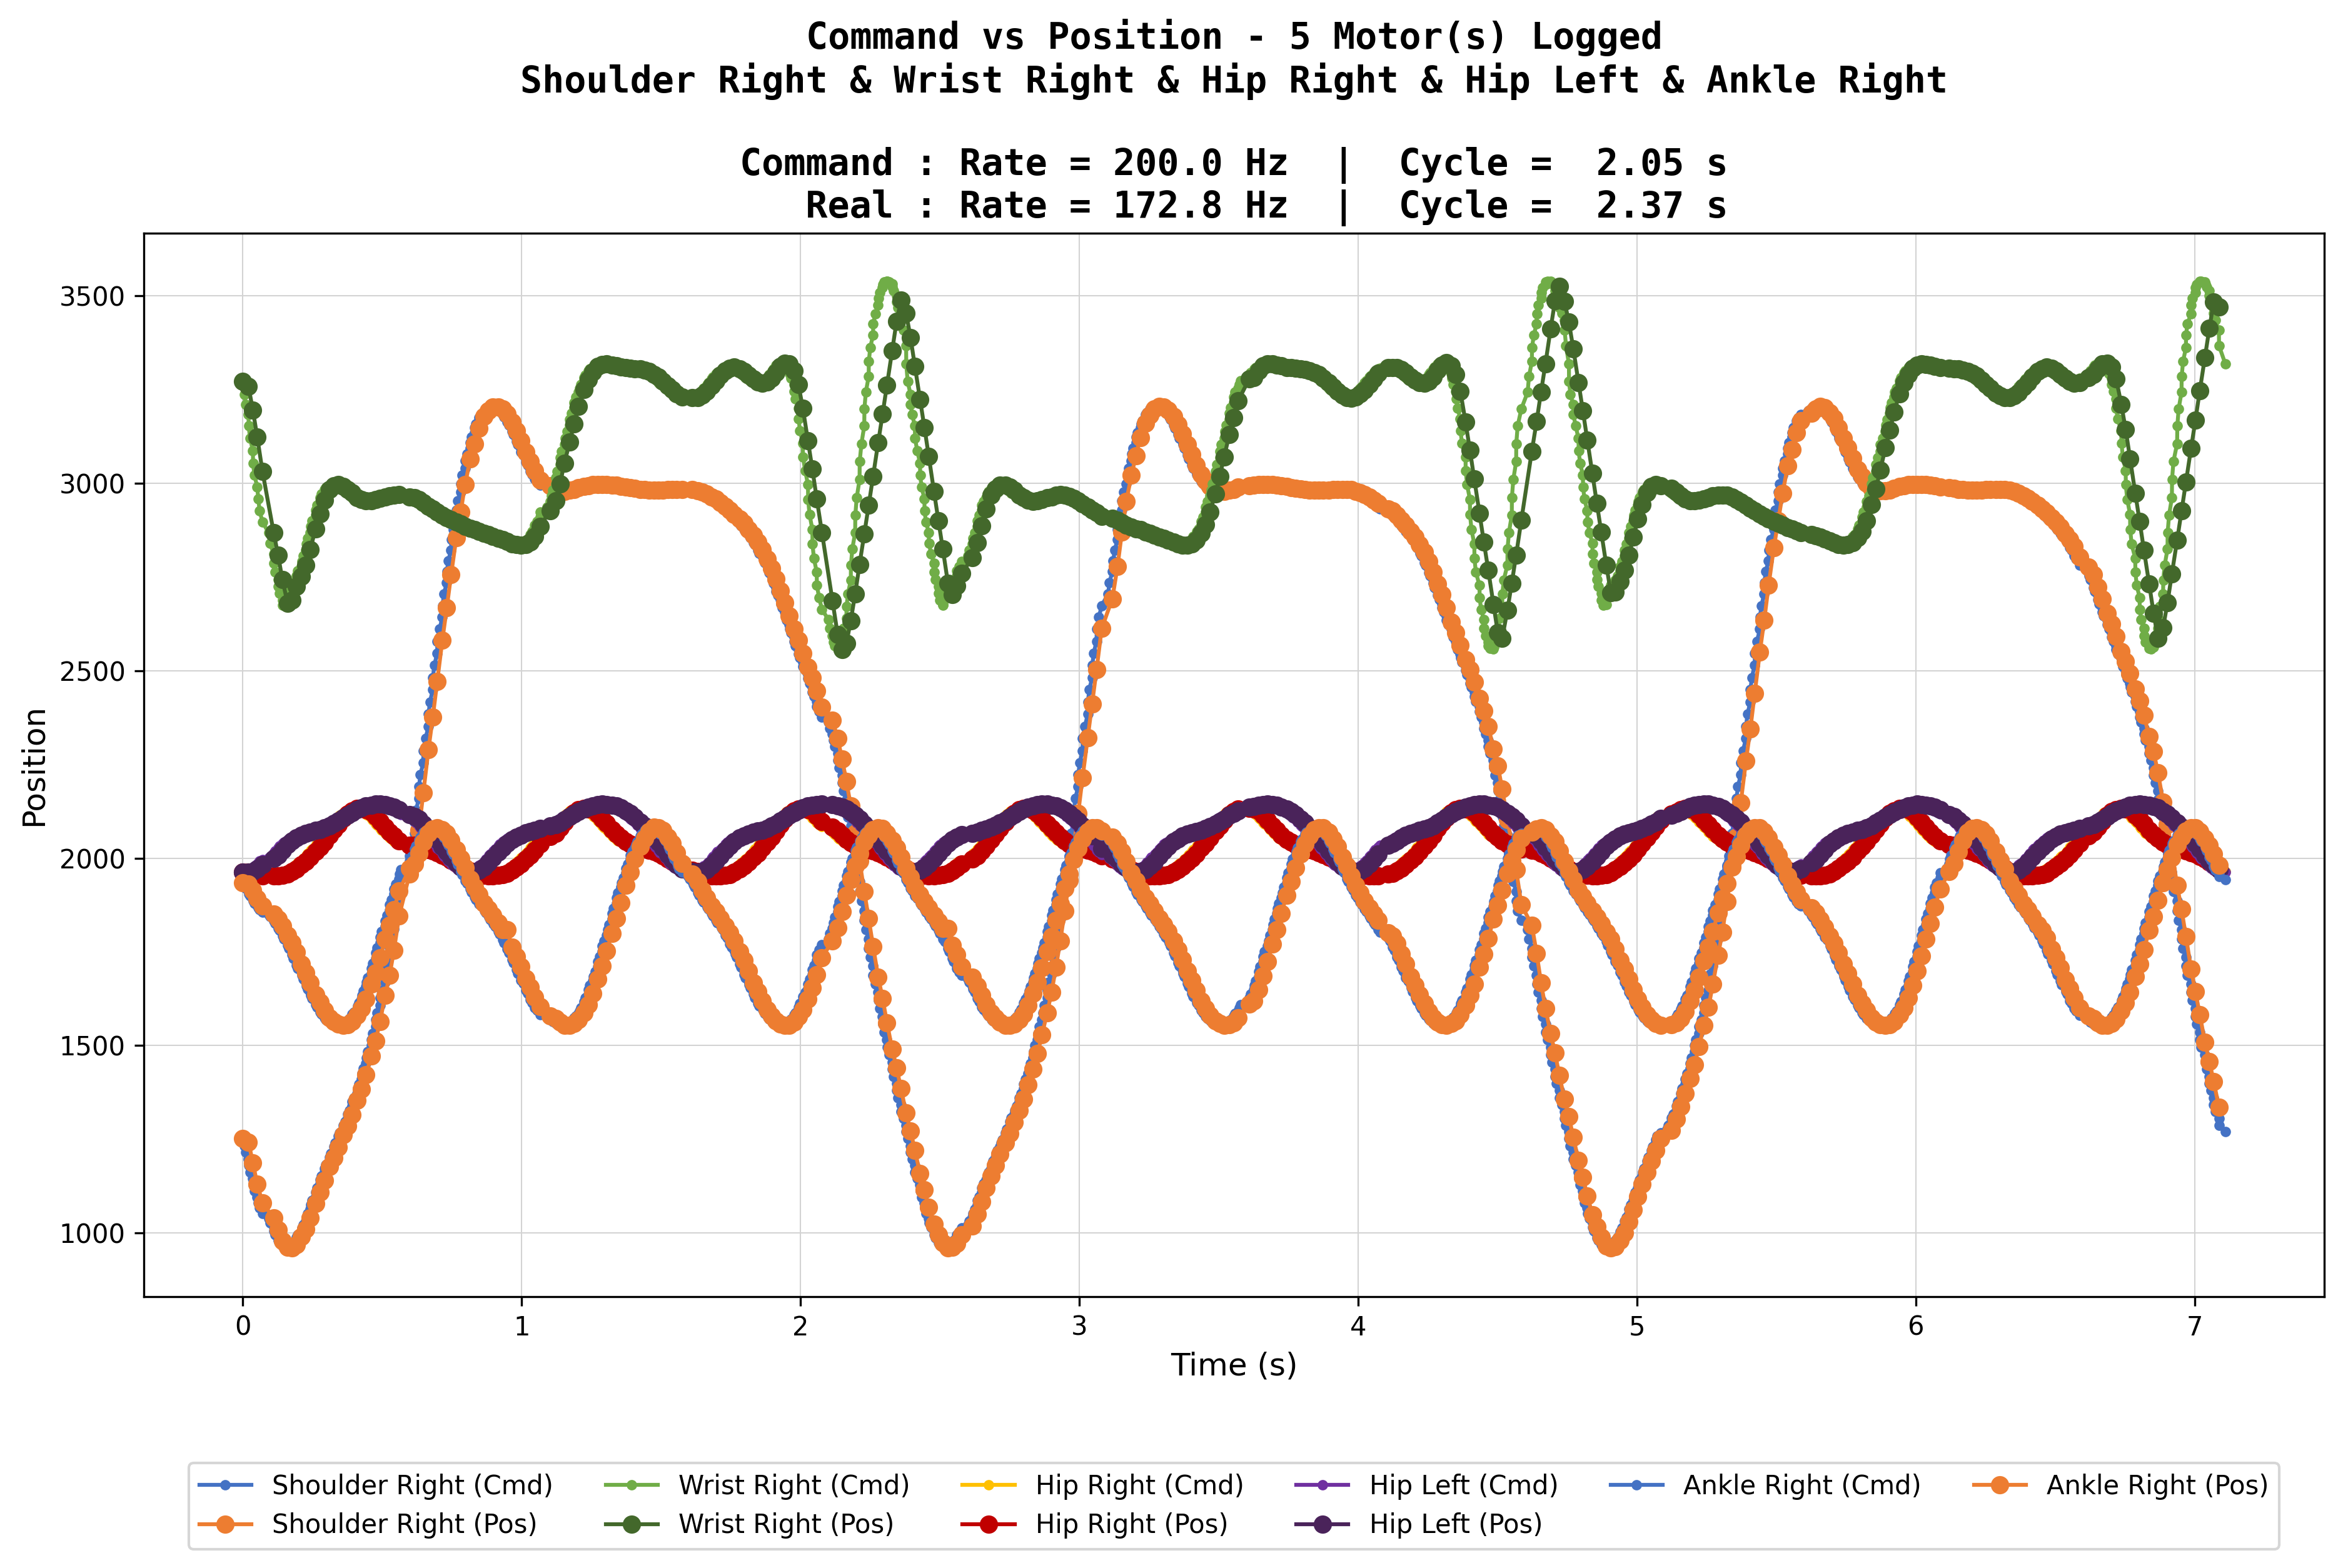
\includegraphics[width=\textwidth]{graphiques/log_5mot_200Hz.png}
        \caption{$N = 5$ motors $\rightarrow$ 172.8 Hz.}
        \label{fig:ssweep5}
    \end{subfigure}
    \caption{Effect of the number of logged motors $N$ on control frequency for 4 and 5 motors (200\,Hz and $K = 3$ frames).}
    \label{fig:sweep_motors_part2}
\end{figure}
\fi

\begin{figure}[H]
    \centering
    \begin{subfigure}[b]{0.49\textwidth}
        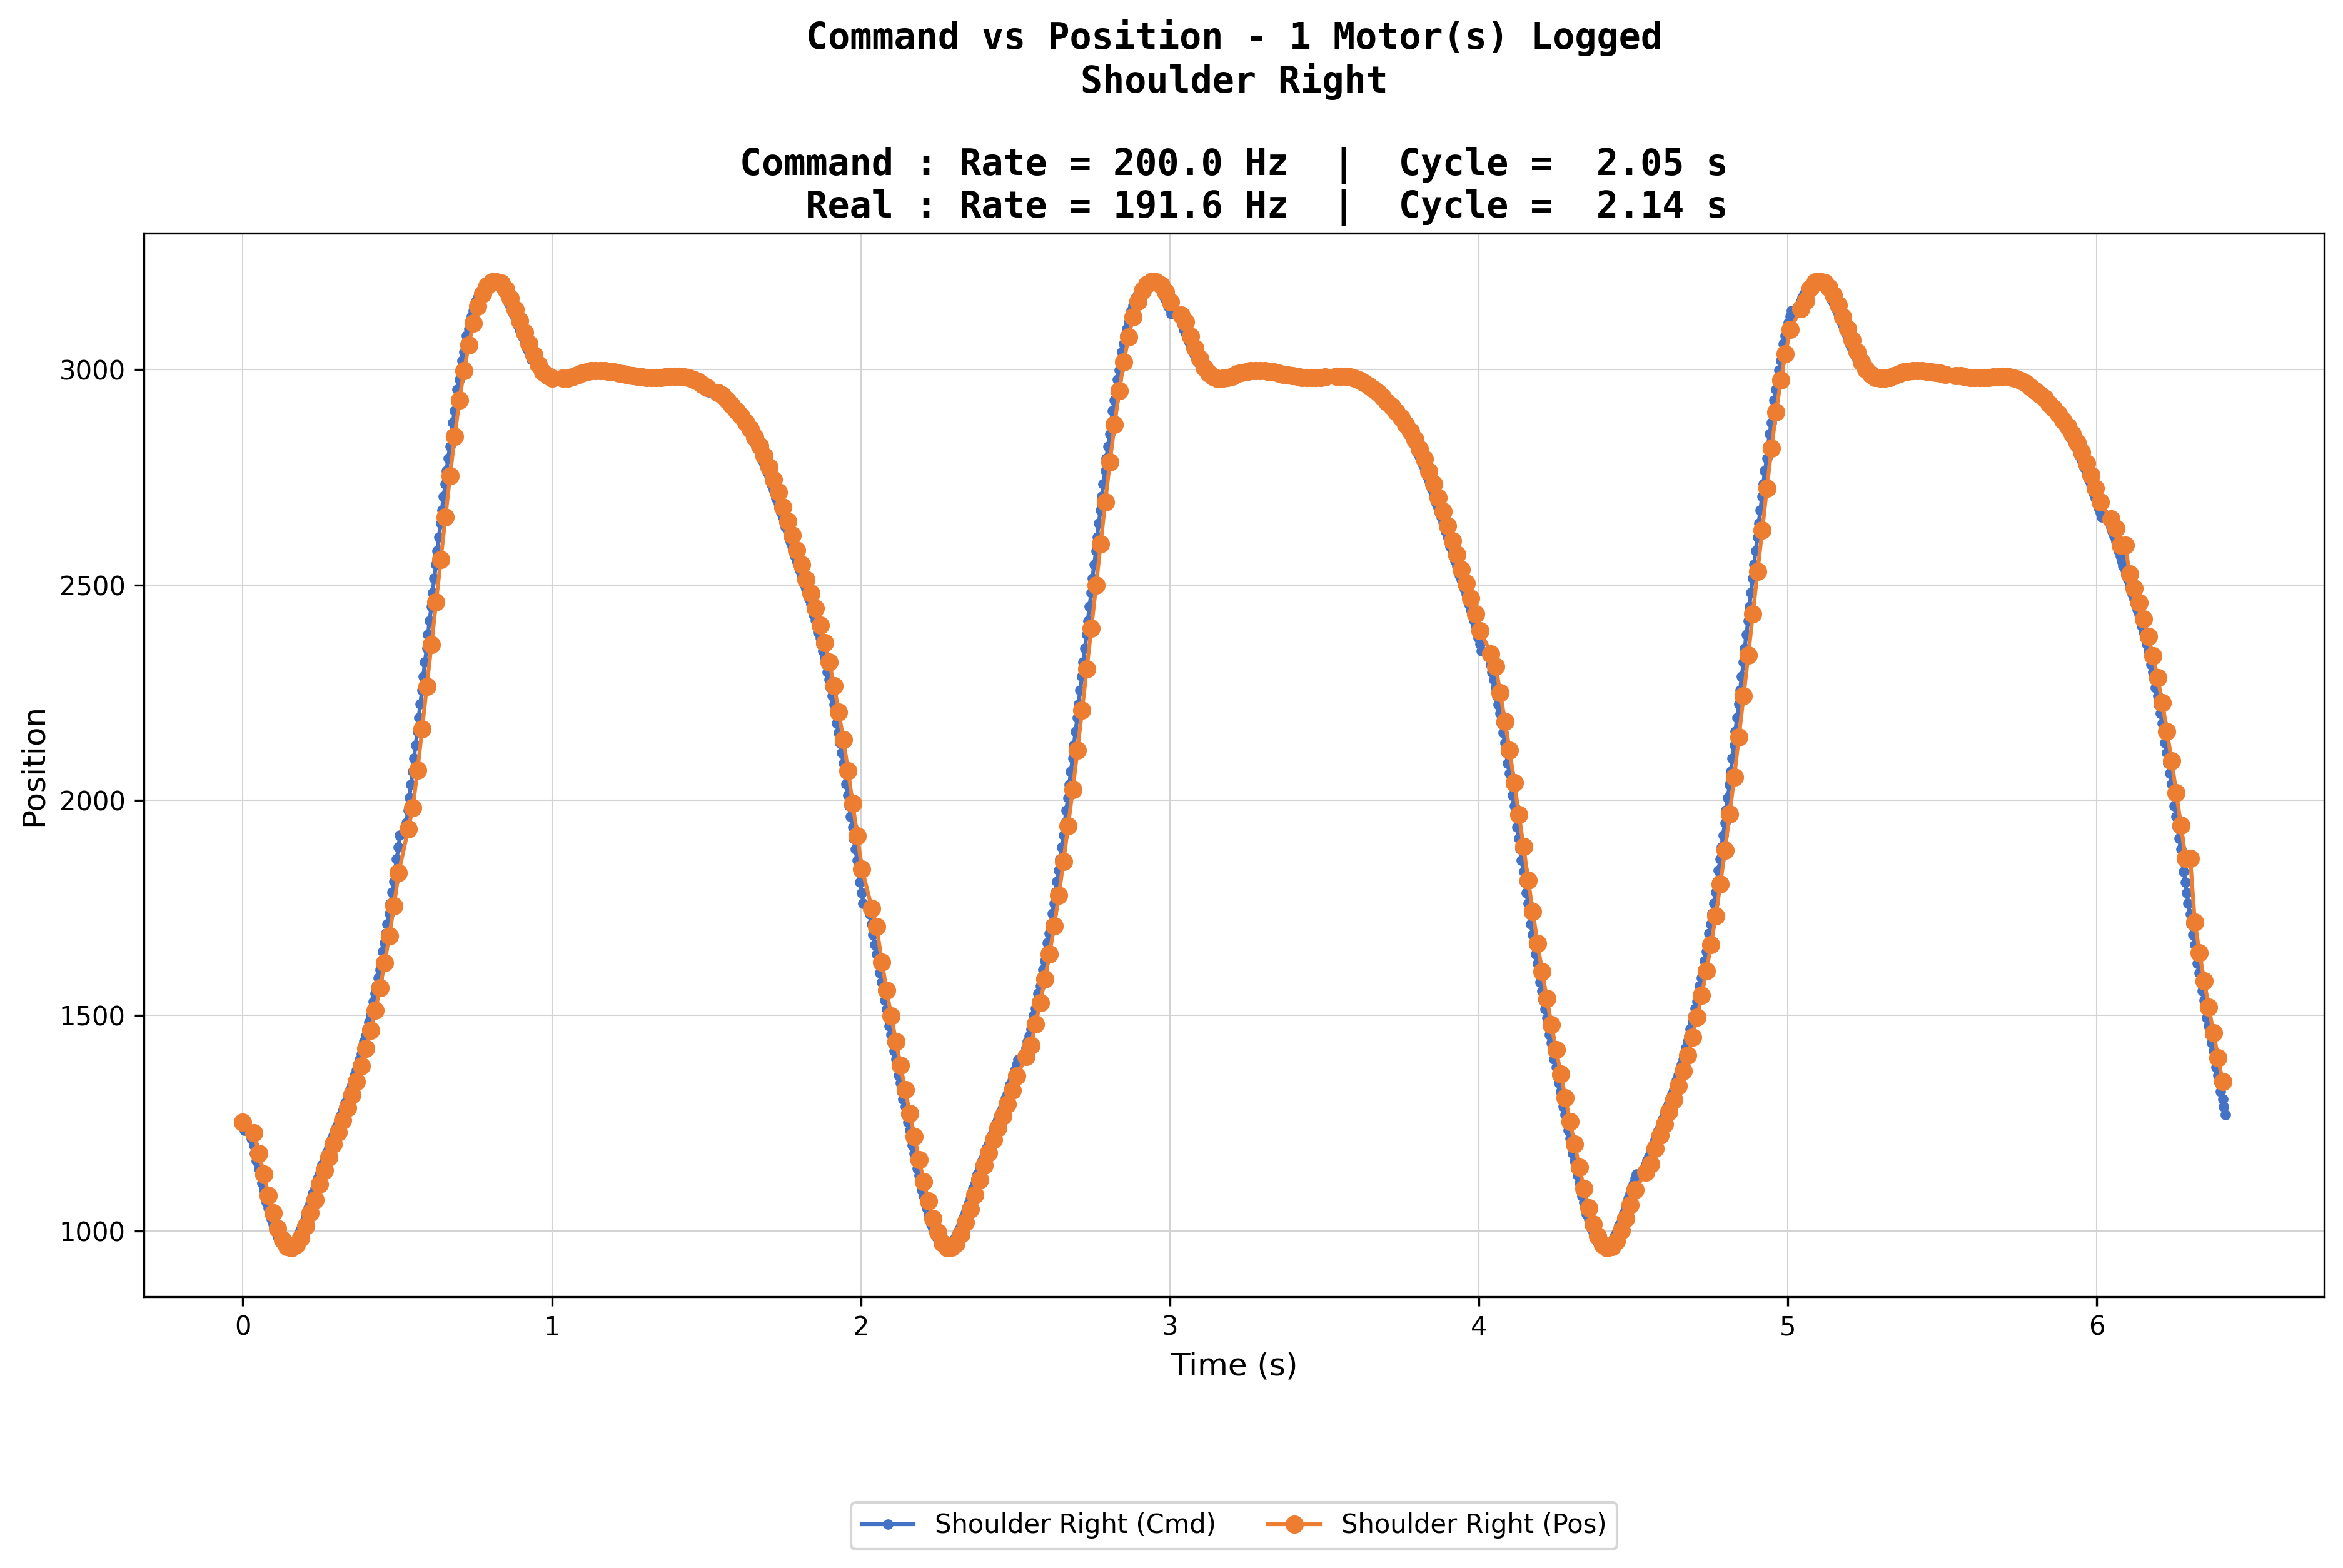
\includegraphics[width=\textwidth]{graphiques/log_1mot_200Hz.png}
        \caption{$N = 1$ motor $\rightarrow$ 191.6 Hz.}
        \label{fig:sweep1}
    \end{subfigure}
    \hfill
    \begin{subfigure}[b]{0.49\textwidth}
        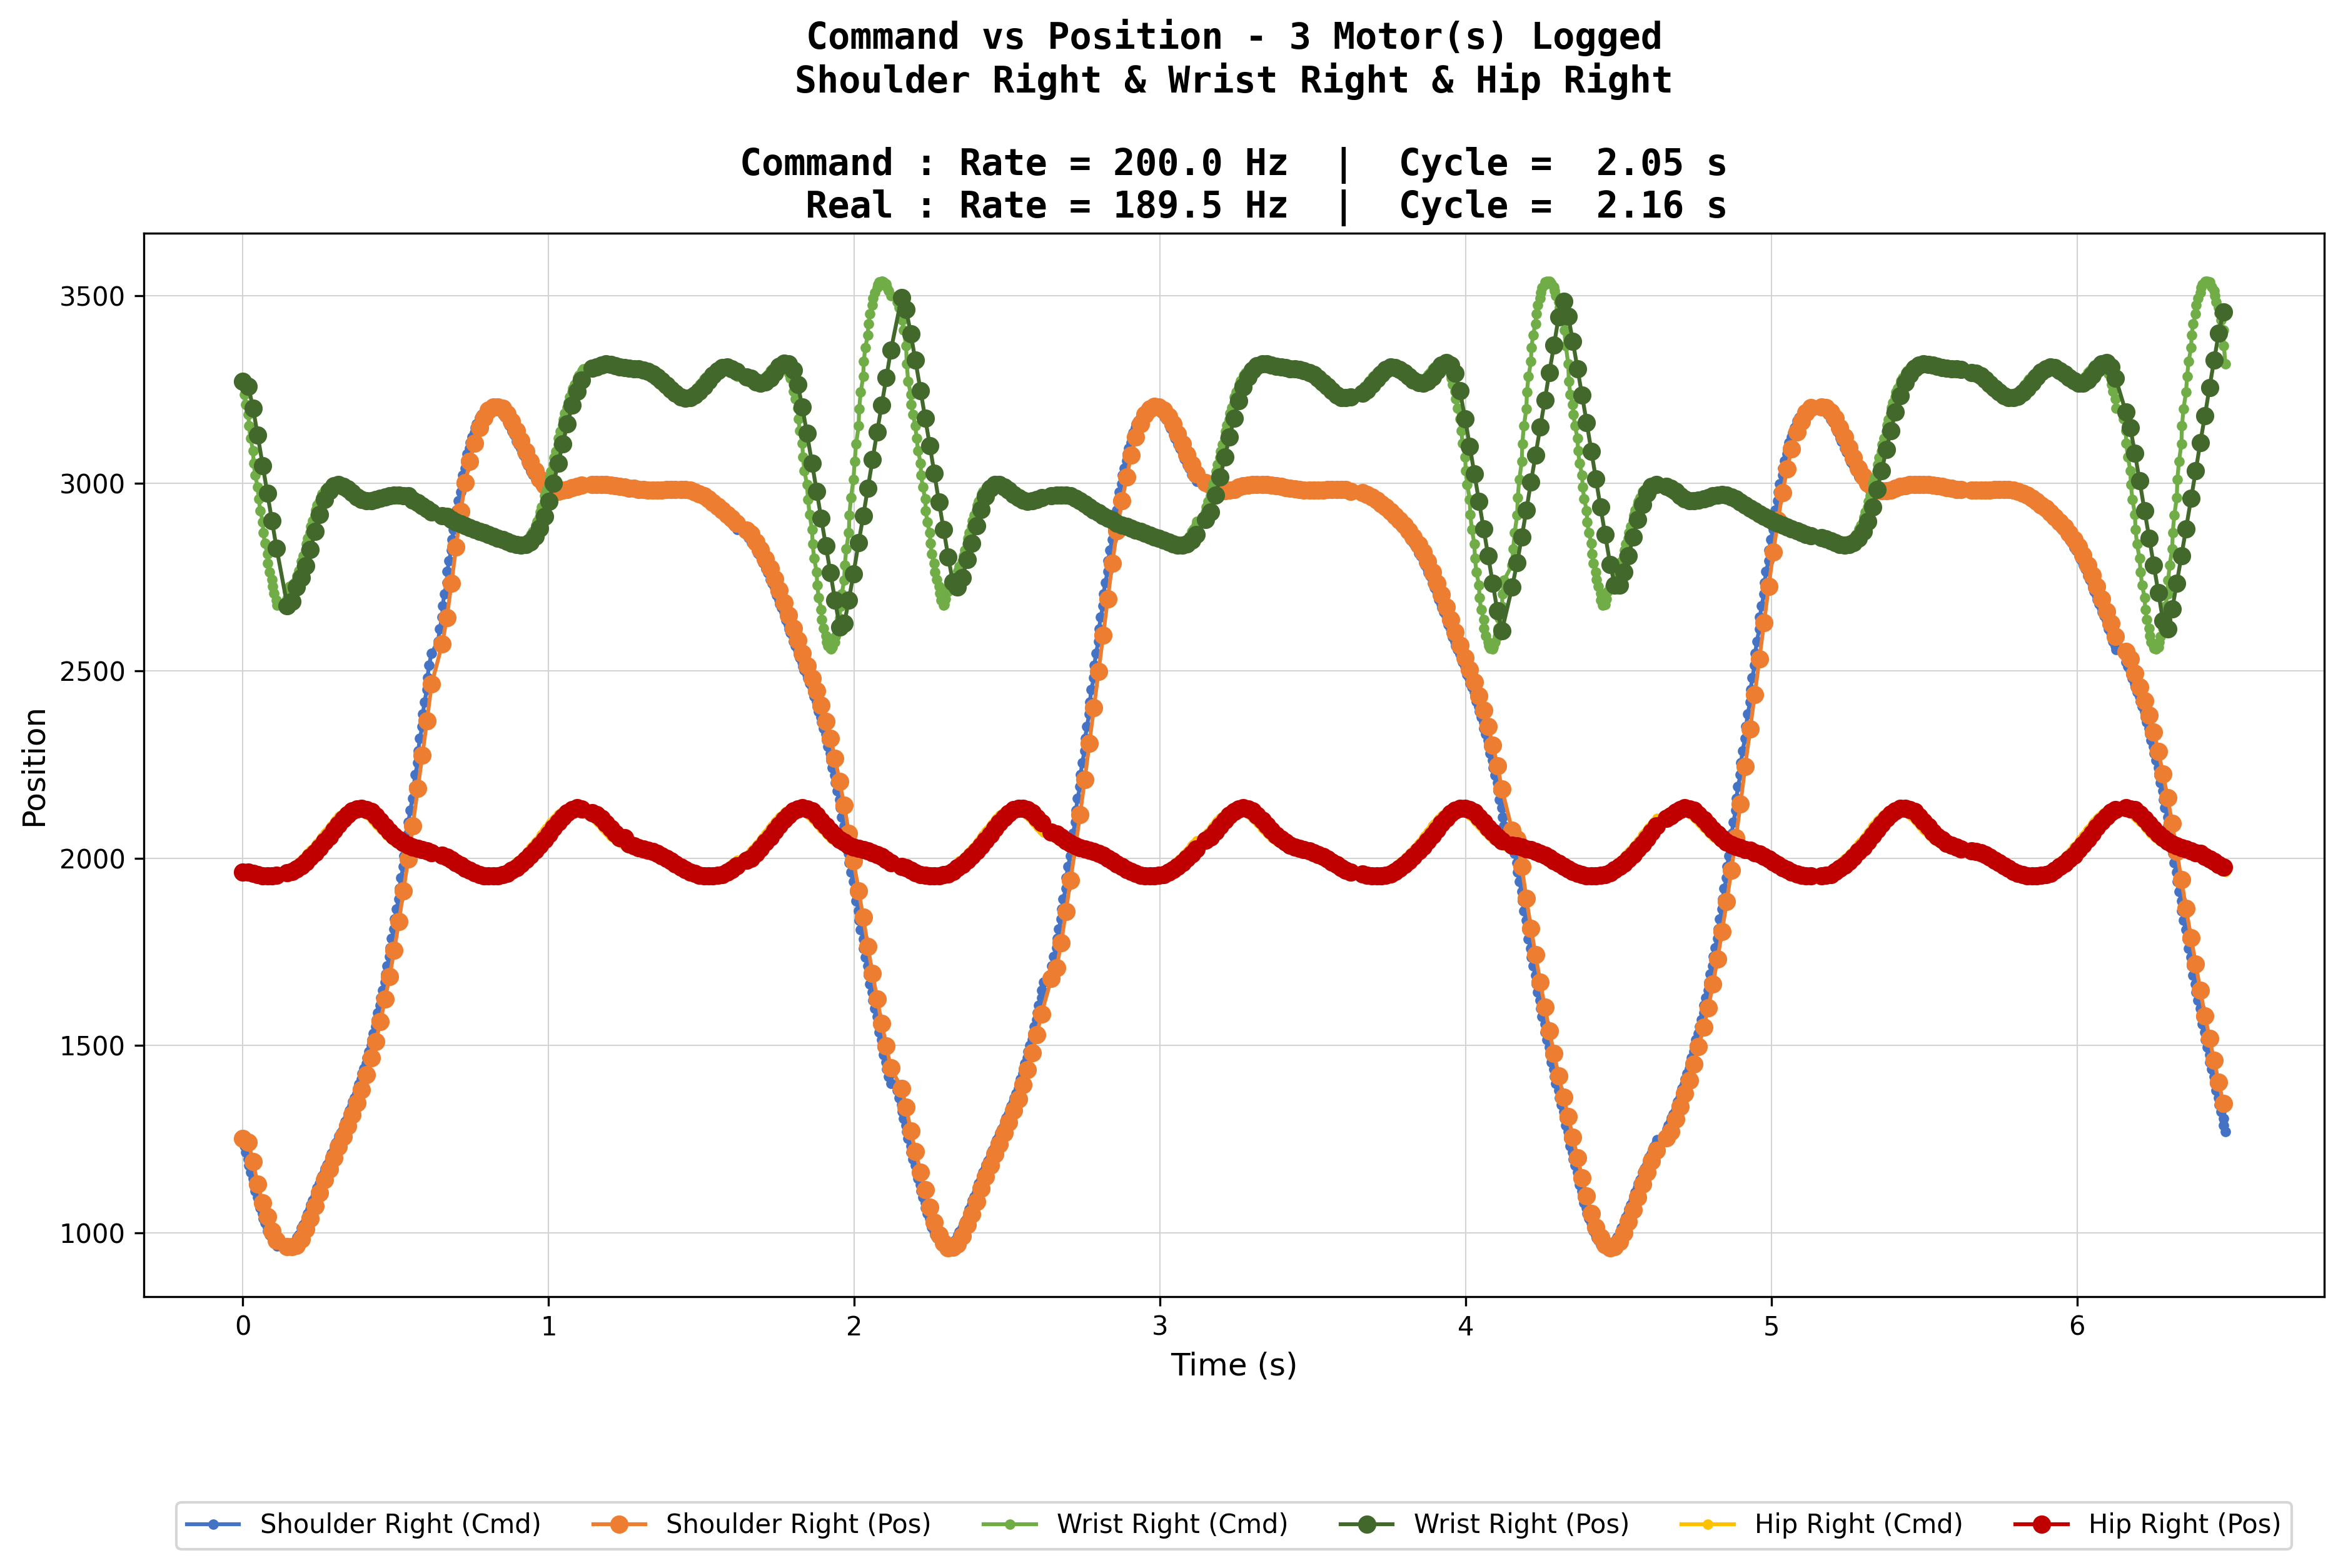
\includegraphics[width=\textwidth]{graphiques/log_3mot_200Hz.png}
        \caption{$N = 3$ motors $\rightarrow$ 189.5 Hz.}
        \label{fig:sweep3}
    \end{subfigure}

    \vspace{0.4em}
    \begin{subfigure}[b]{0.49\textwidth}
        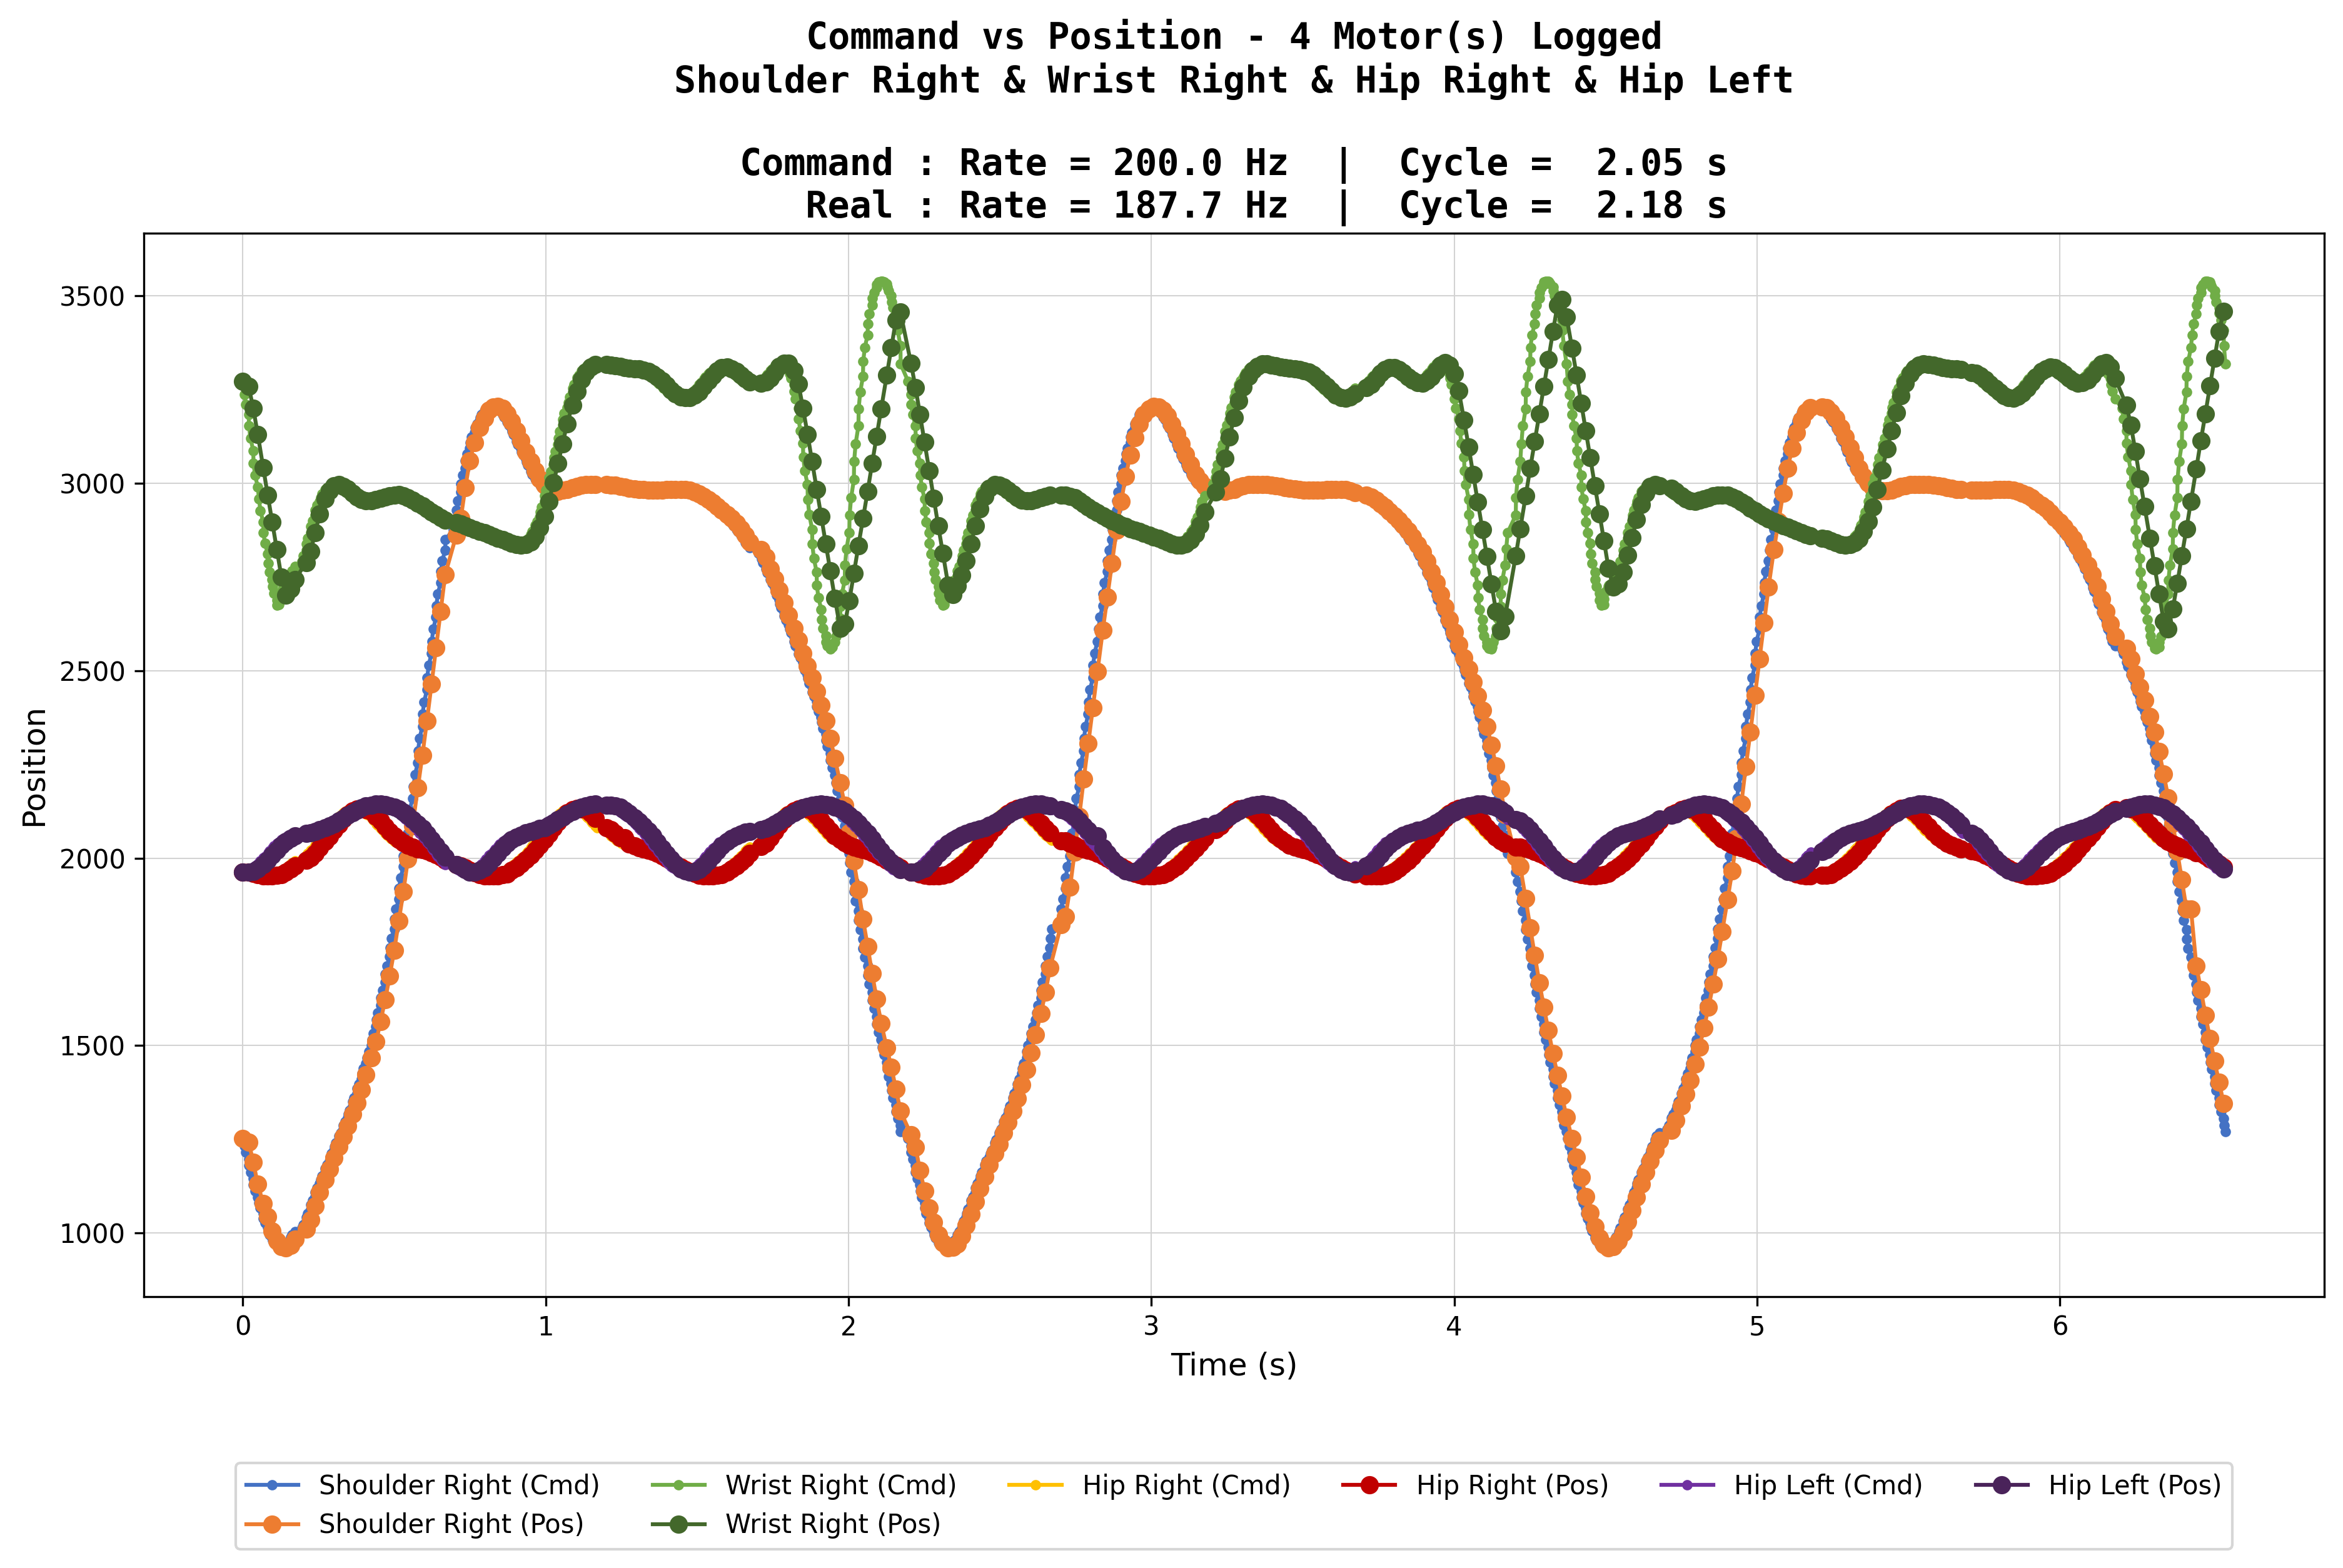
\includegraphics[width=\textwidth]{graphiques/log_4mot_200Hz.png}
        \caption{$N = 4$ motors $\rightarrow$ 187.7 Hz.}
        \label{fig:sweep4}
    \end{subfigure}
    \hfill
    \begin{subfigure}[b]{0.49\textwidth}
        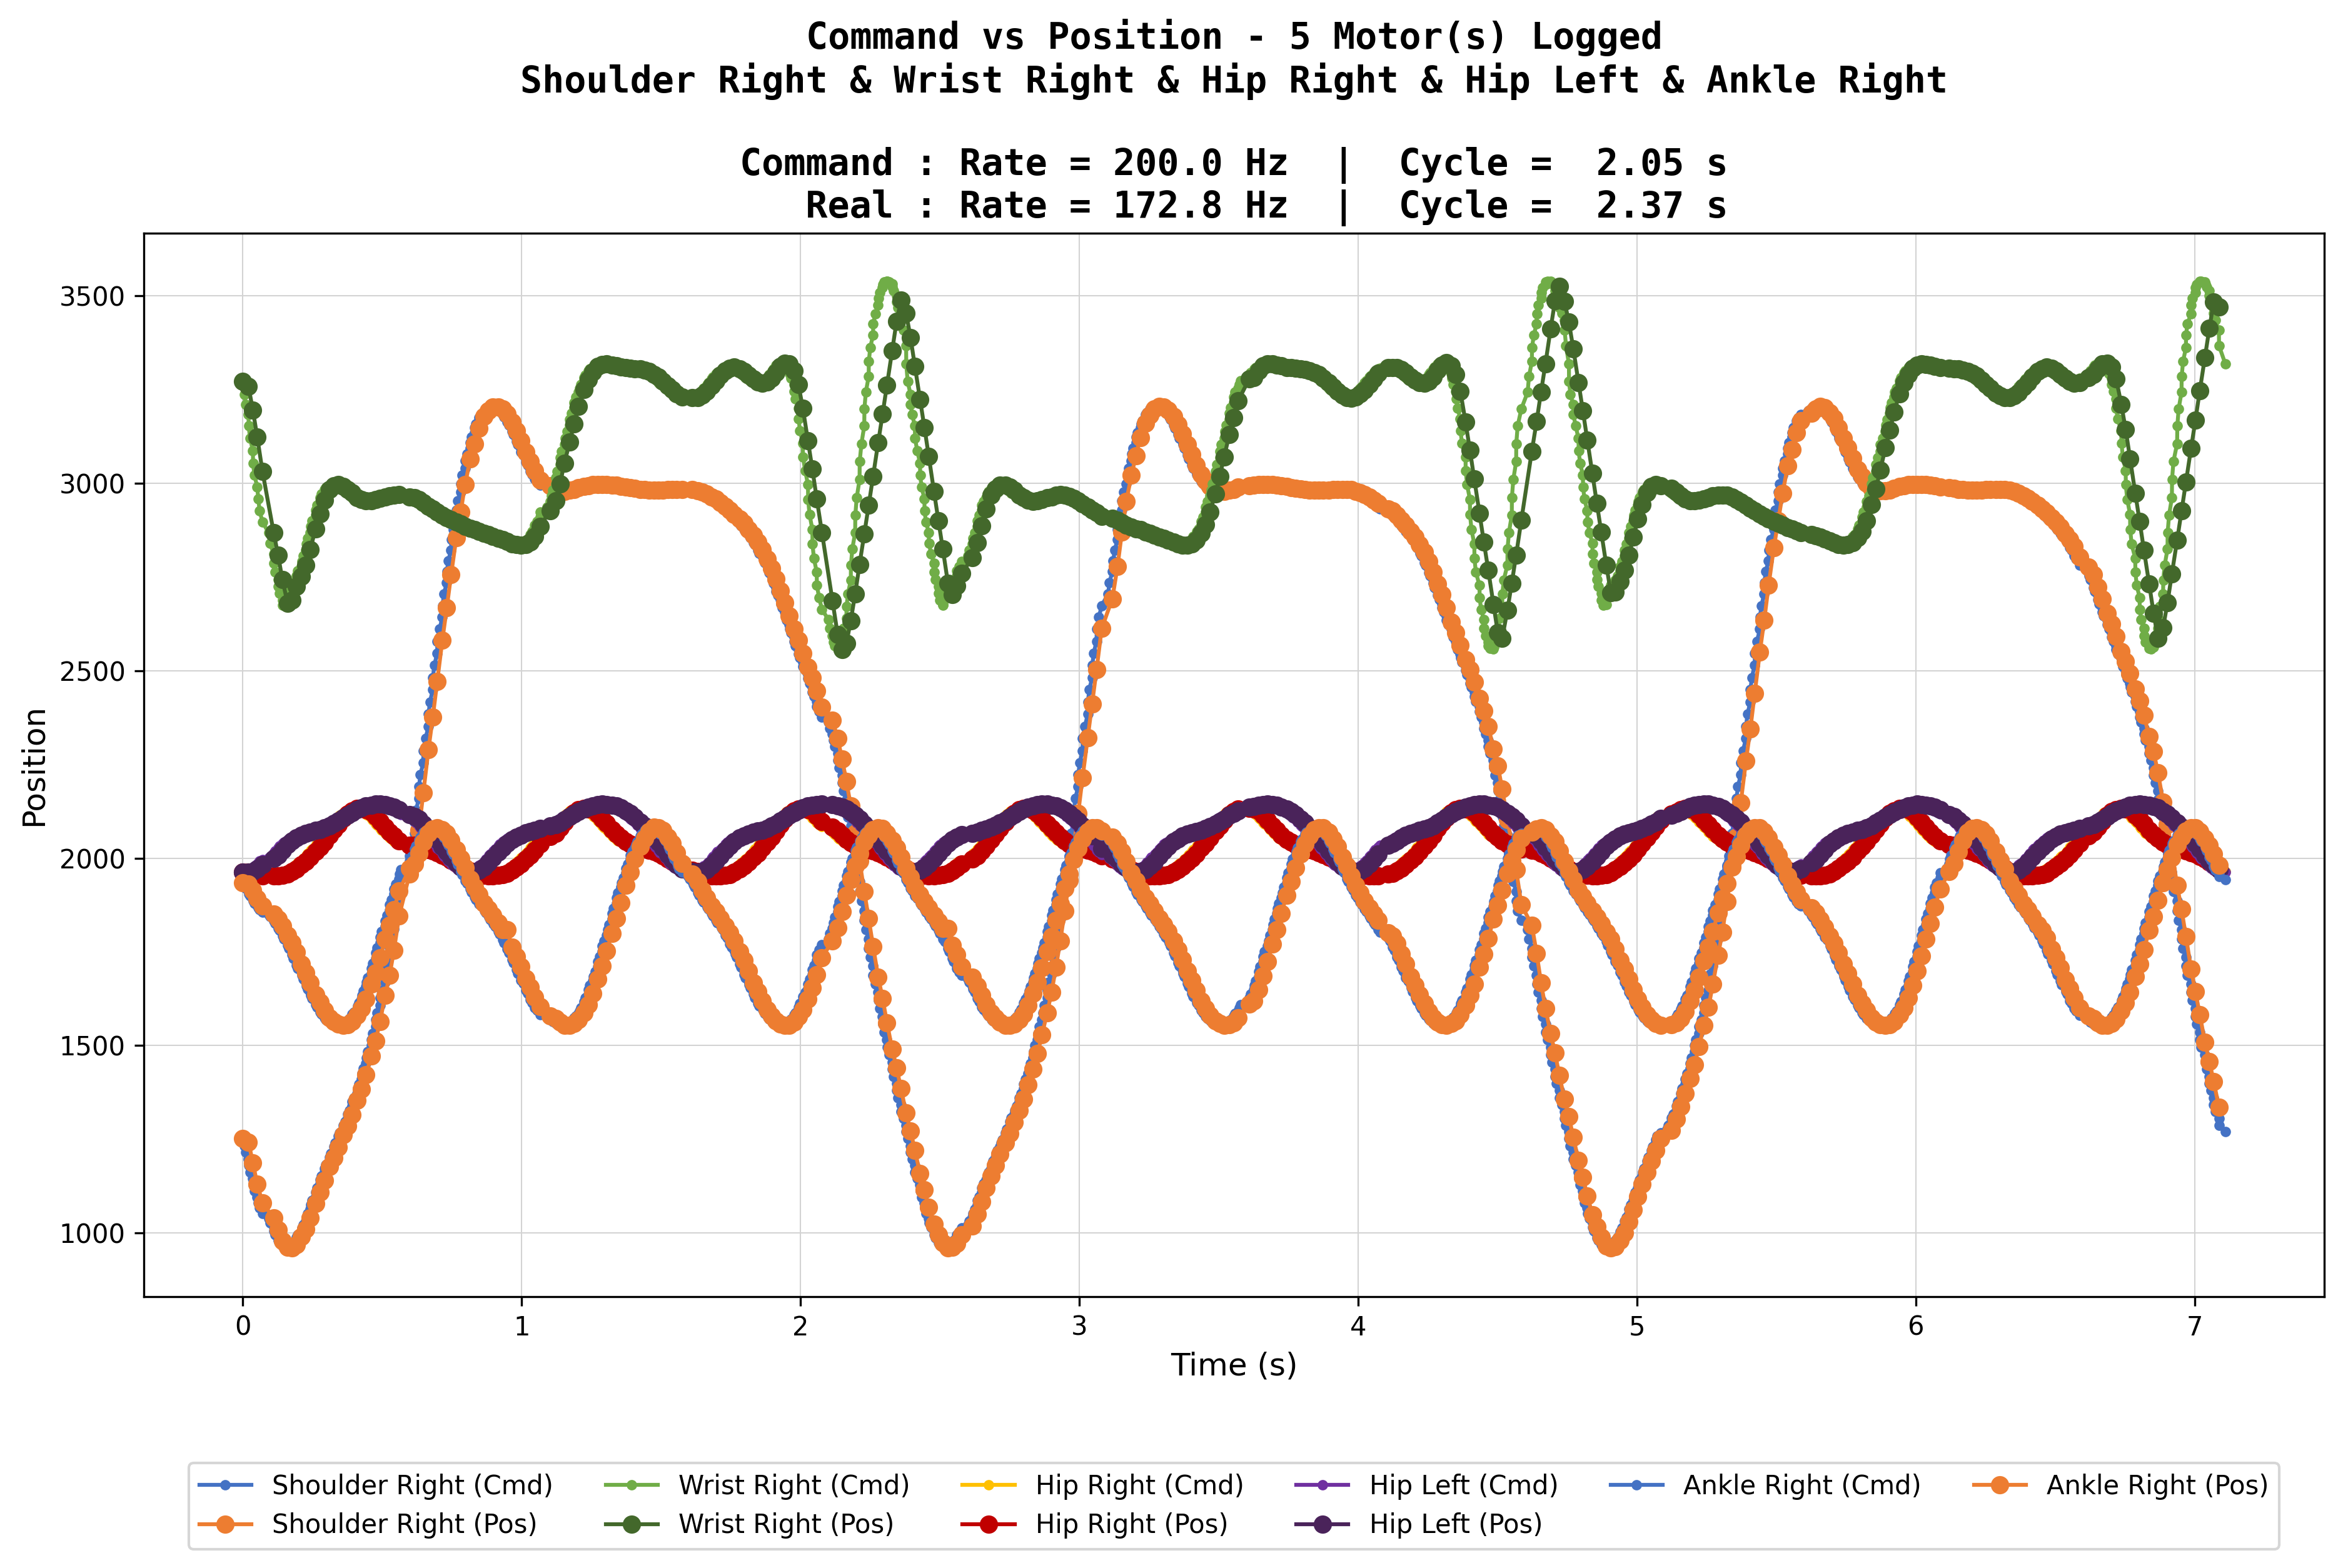
\includegraphics[width=\textwidth]{graphiques/log_5mot_200Hz.png}
        \caption{$N = 5$ motors $\rightarrow$ 172.8 Hz.}
        \label{fig:sweep5}
    \end{subfigure}
    \caption{Effect of the number of logged motors $N$ on control frequency (200\,Hz and $K = 3$ frames).}
    \label{fig:sweep_motors}
\end{figure}


\vspace{-0.2cm}

As we can see in the figure~\ref{fig:sweep_motors}, the control frequency drops from 191.6\,Hz with a single motor to 172.8\,Hz with five, with a particularly sharp fall at the fifth. So the \emph{tracking} stays excellent in every case and only the loop \emph{rate} is affected, not the command/position fidelity. Looking at this result we can wonder if this degradation is an inevitable price of logging, or does it appear only in a particular regime. To settle it, I reran the exact same campaign at lower setpoint rates, at 36, 72 and 100\,Hz :

\iffalse
\begin{figure}[H]
    \centering
    \begin{subfigure}[b]{0.48\textwidth}
        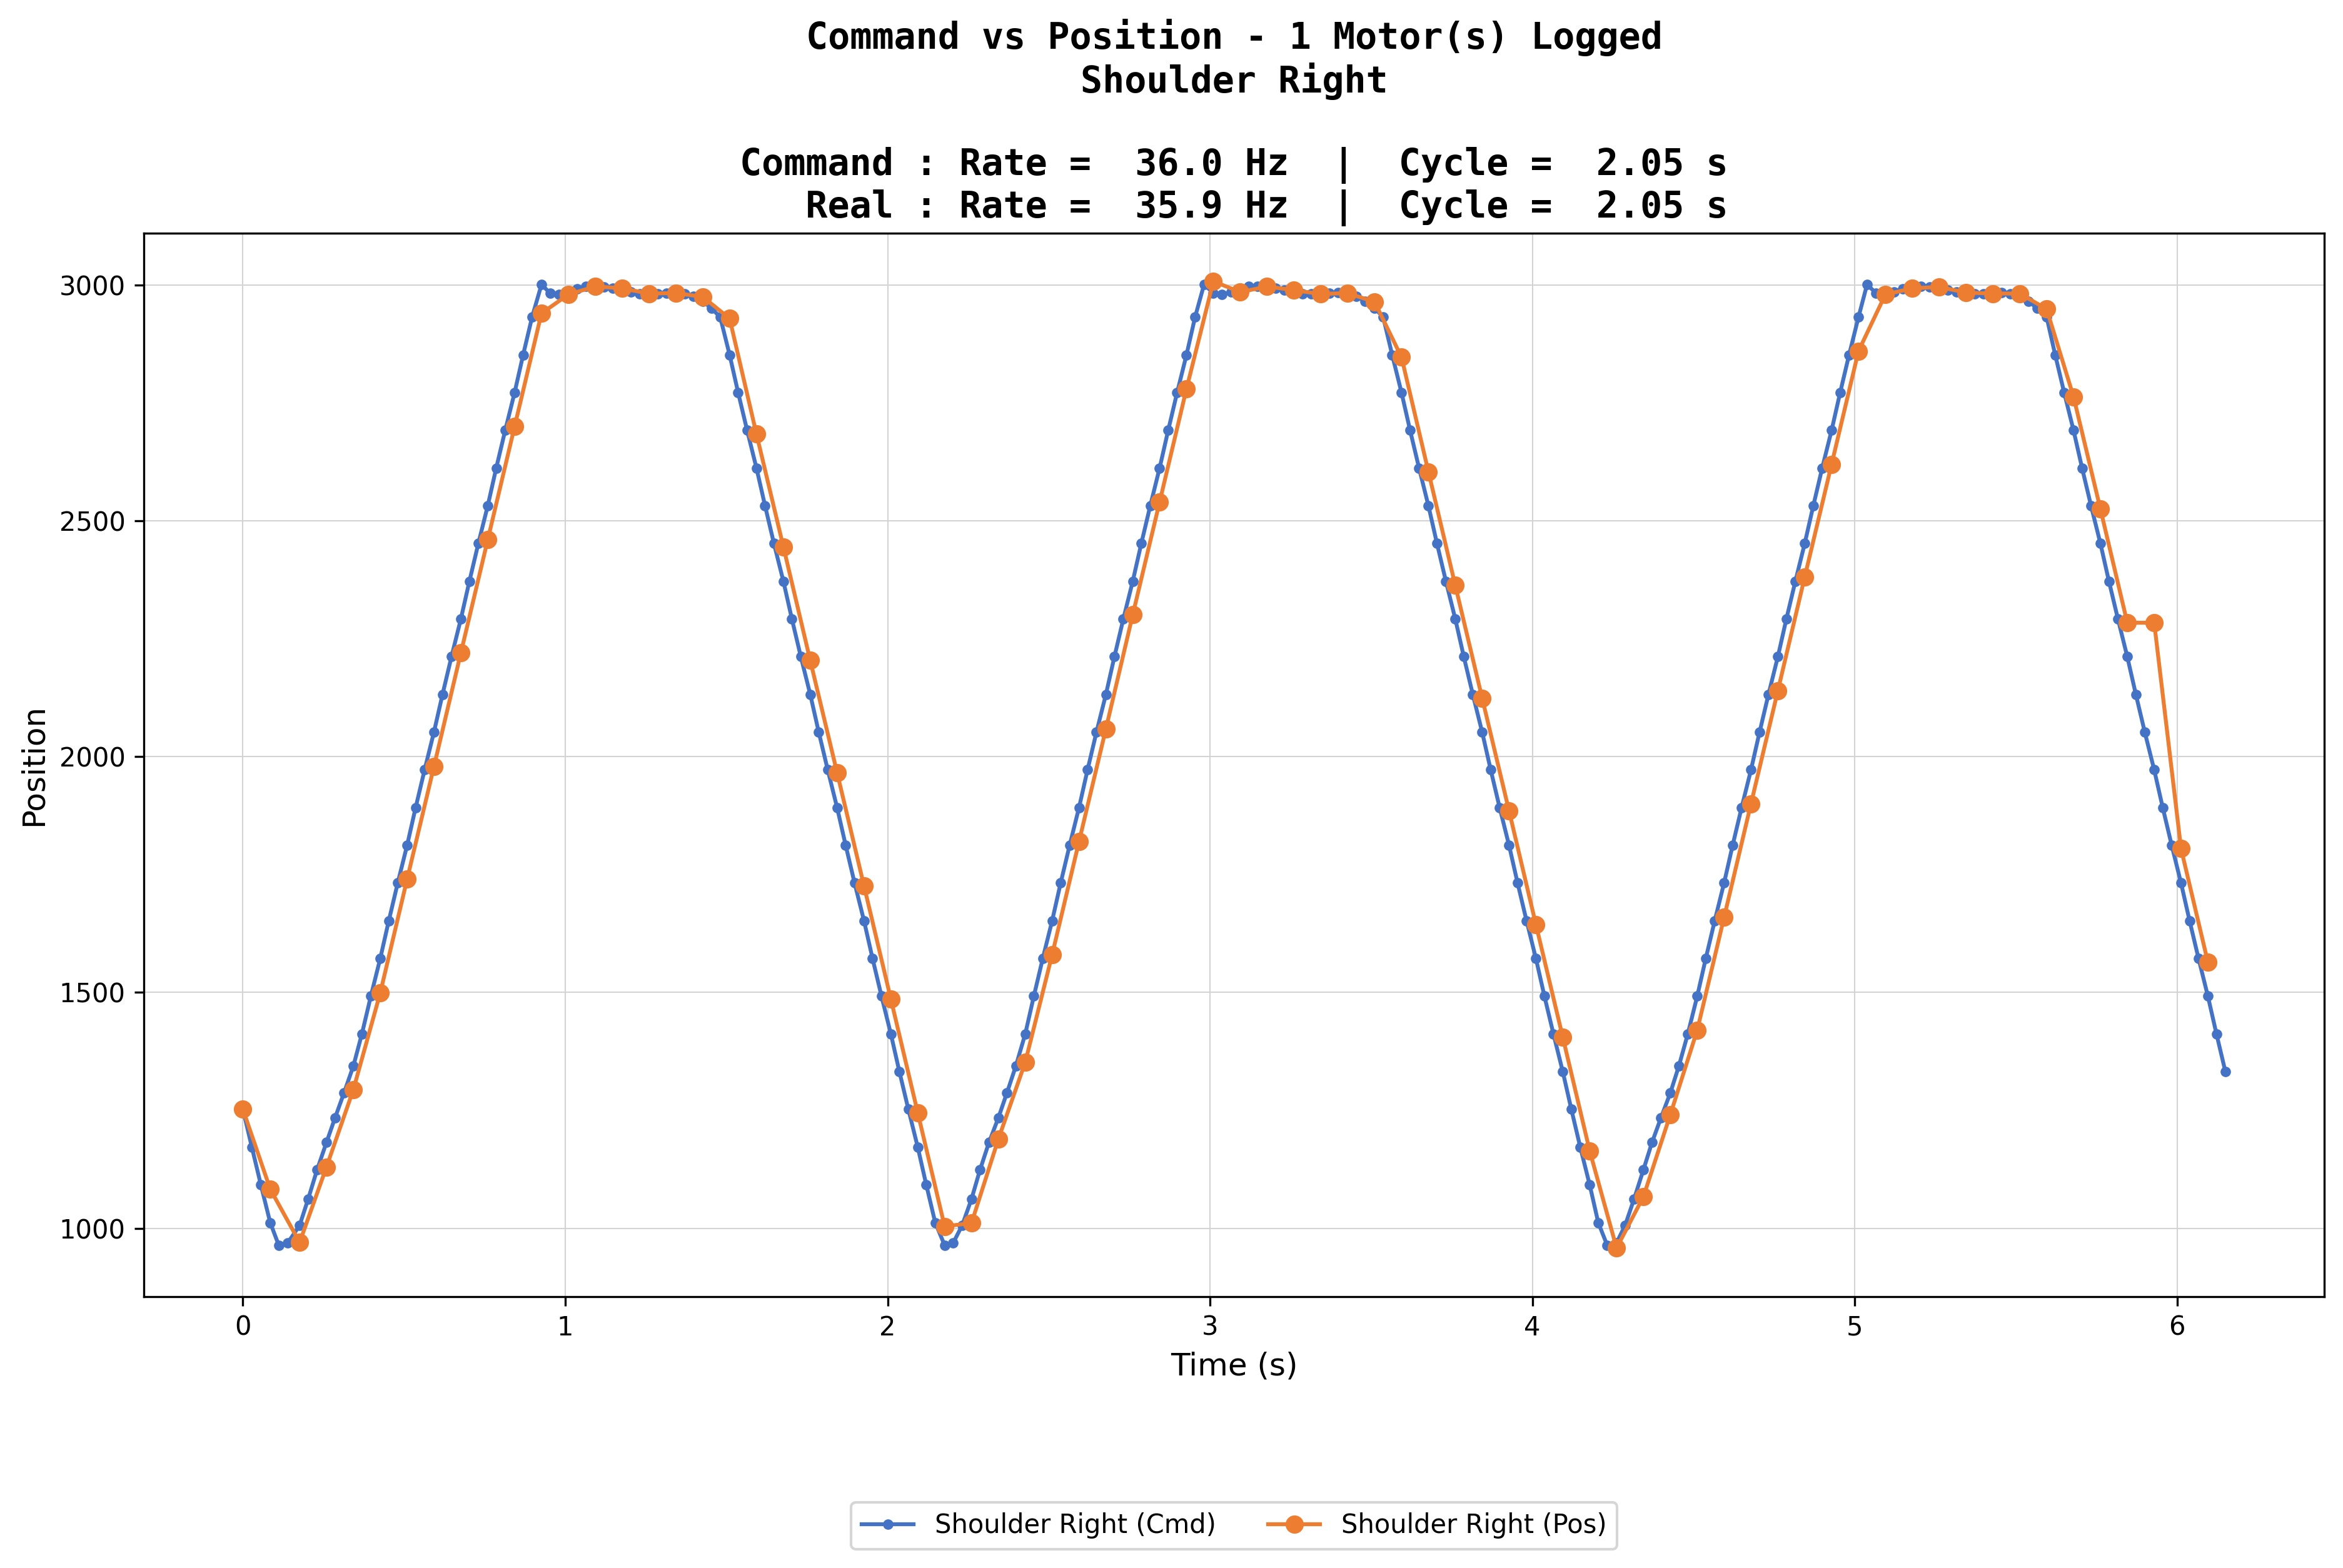
\includegraphics[width=\textwidth]{graphiques/log_36Hz_1mot.png}
        \caption{36\,Hz, $N = 1$ $\rightarrow$ 35.9 Hz.}
    \end{subfigure}
    \hfill
    \begin{subfigure}[b]{0.48\textwidth}
        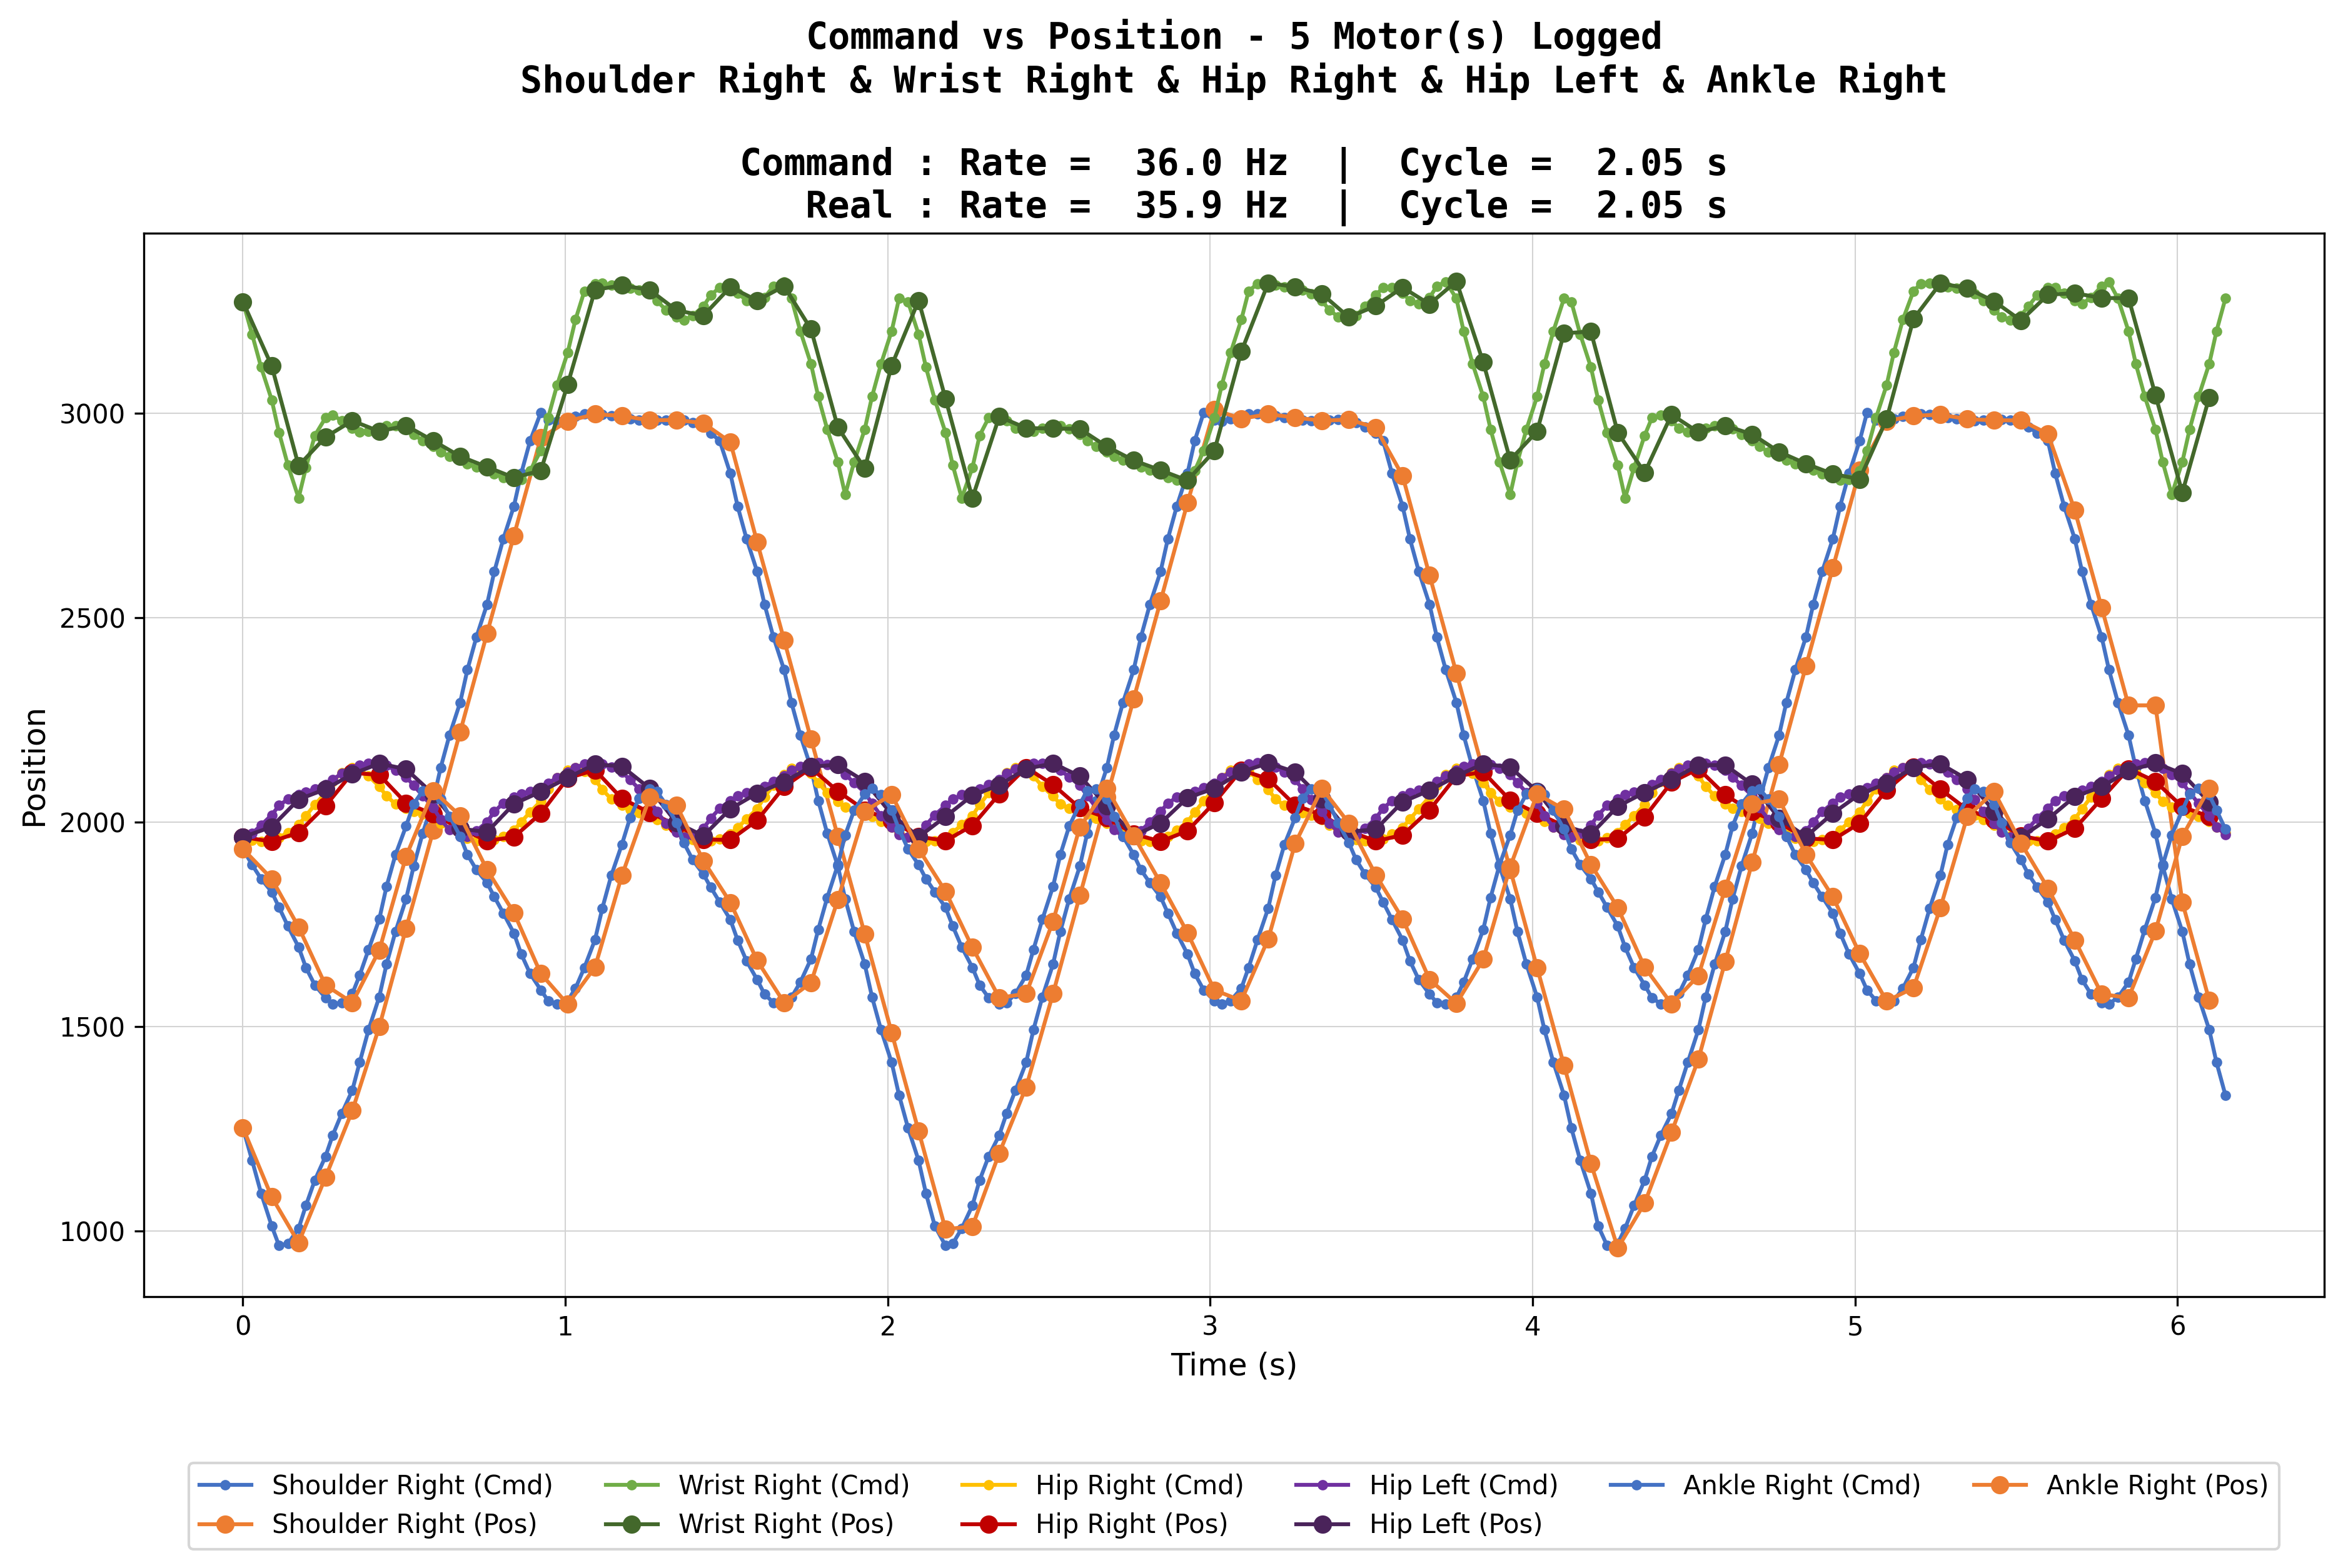
\includegraphics[width=\textwidth]{graphiques/log_36Hz_5mot.png}
        \caption{36\,Hz, $N = 5$ $\rightarrow$ 35.9 Hz.}
    \end{subfigure}
    \caption{Sweep of the number of logged motors at 36 Hz.}
    \label{fig:lowfreq}
\end{figure}

\begin{figure}[H]
    \centering
    \begin{subfigure}[b]{0.48\textwidth}
        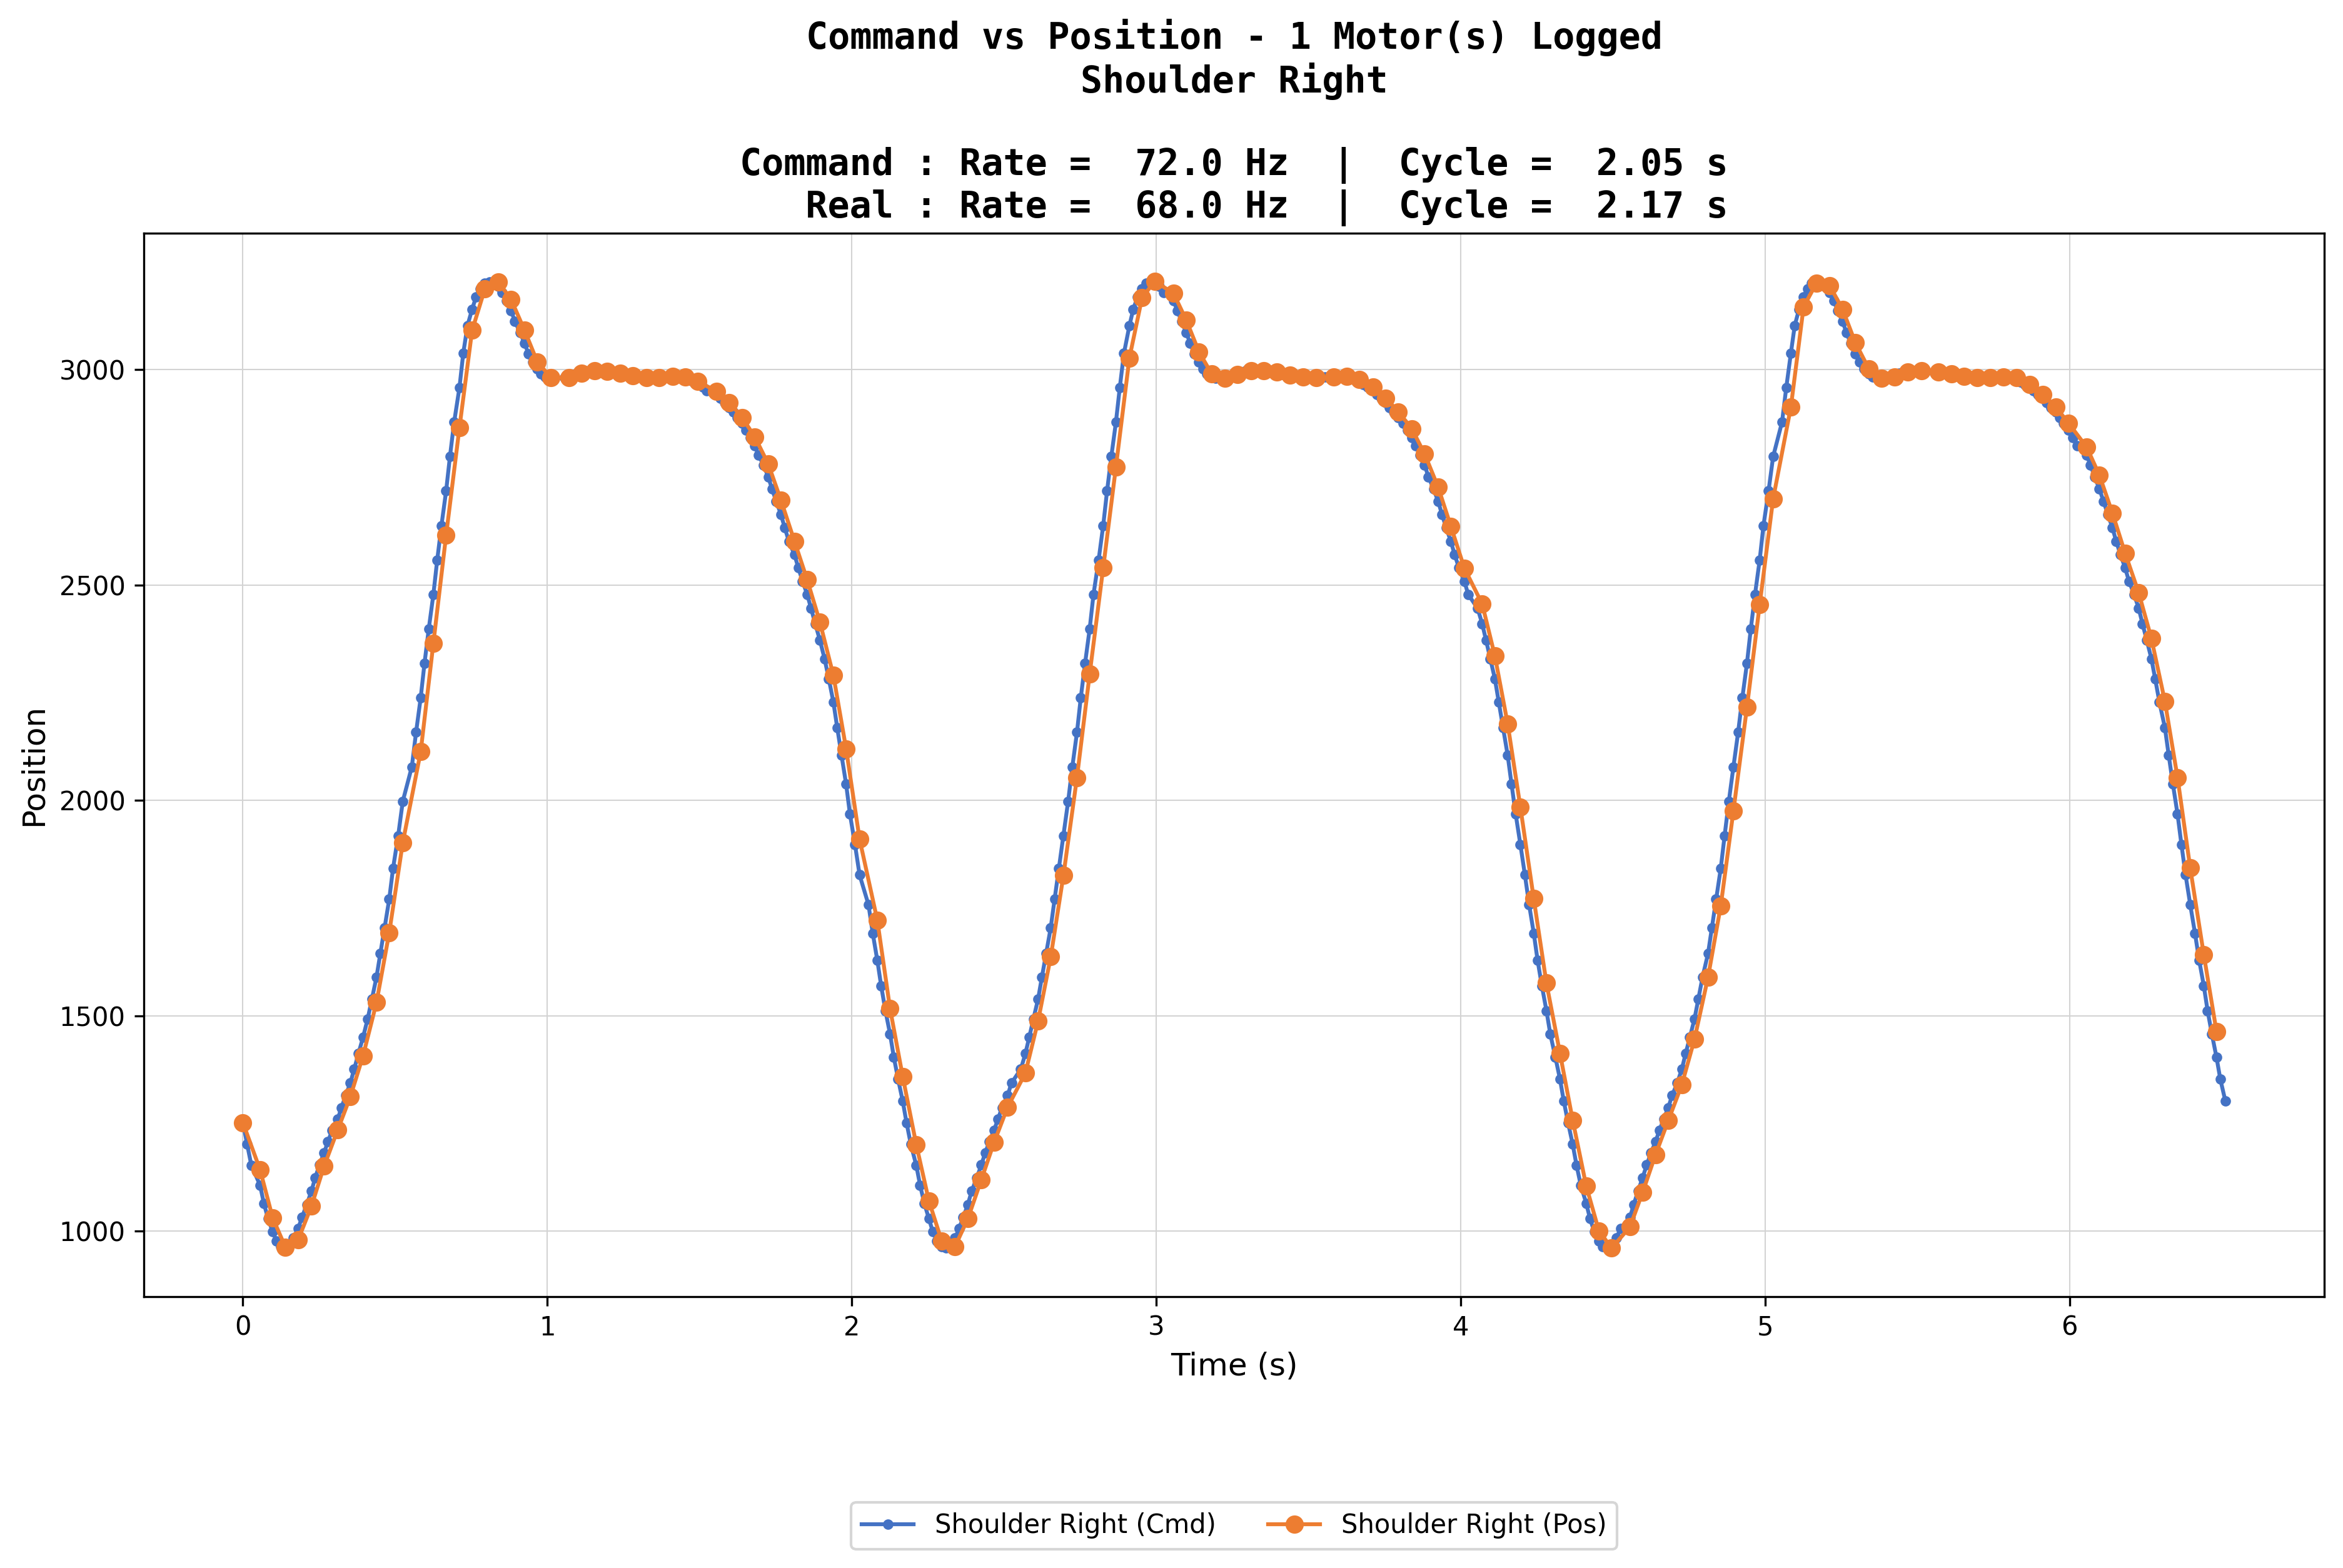
\includegraphics[width=\textwidth]{graphiques/log_72Hz_1mot.png}
        \caption{72\,Hz, $N = 1$ $\rightarrow$ 68.0 Hz.}
    \end{subfigure}
    \hfill
    \begin{subfigure}[b]{0.48\textwidth}
        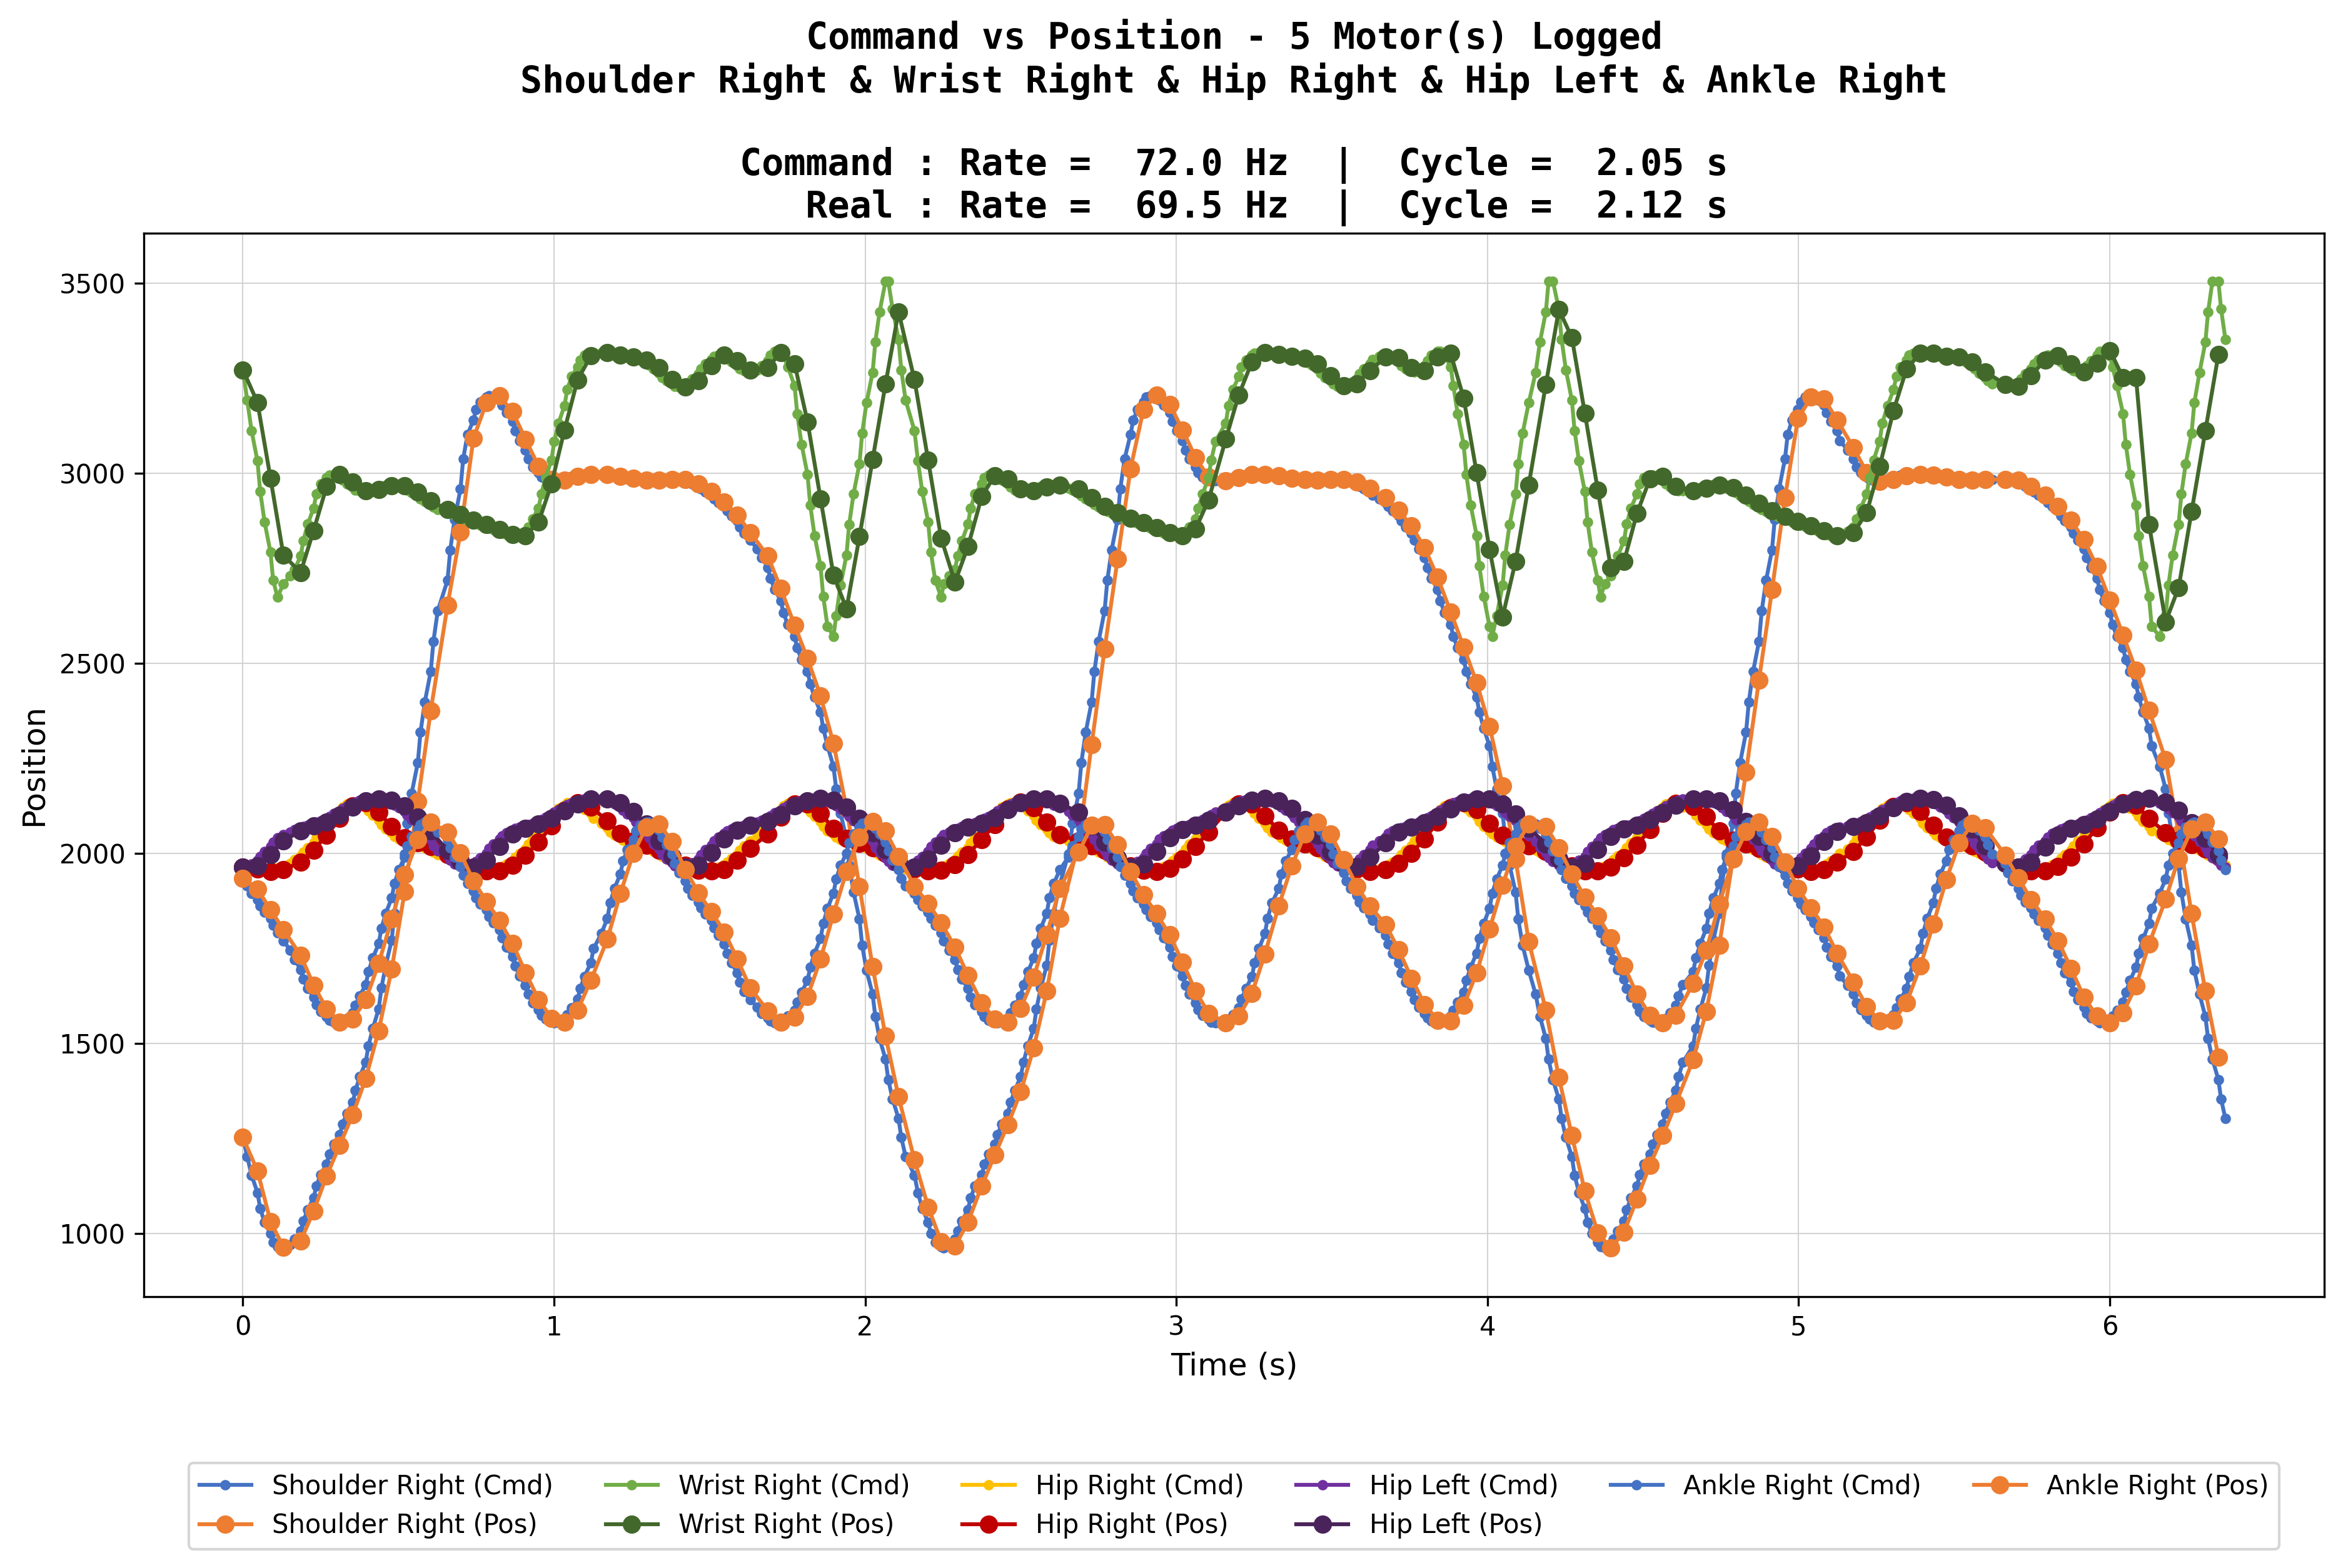
\includegraphics[width=\textwidth]{graphiques/log_72Hz_5mot.png}
        \caption{72\,Hz, $N = 5$ $\rightarrow$ 69.5 Hz.}
    \end{subfigure}
    \caption{Sweep of the number of logged motors at 72 Hz.}
    \label{fig:midfreq}
\end{figure}

\begin{figure}[H]
    \centering
    \begin{subfigure}[b]{0.48\textwidth}
        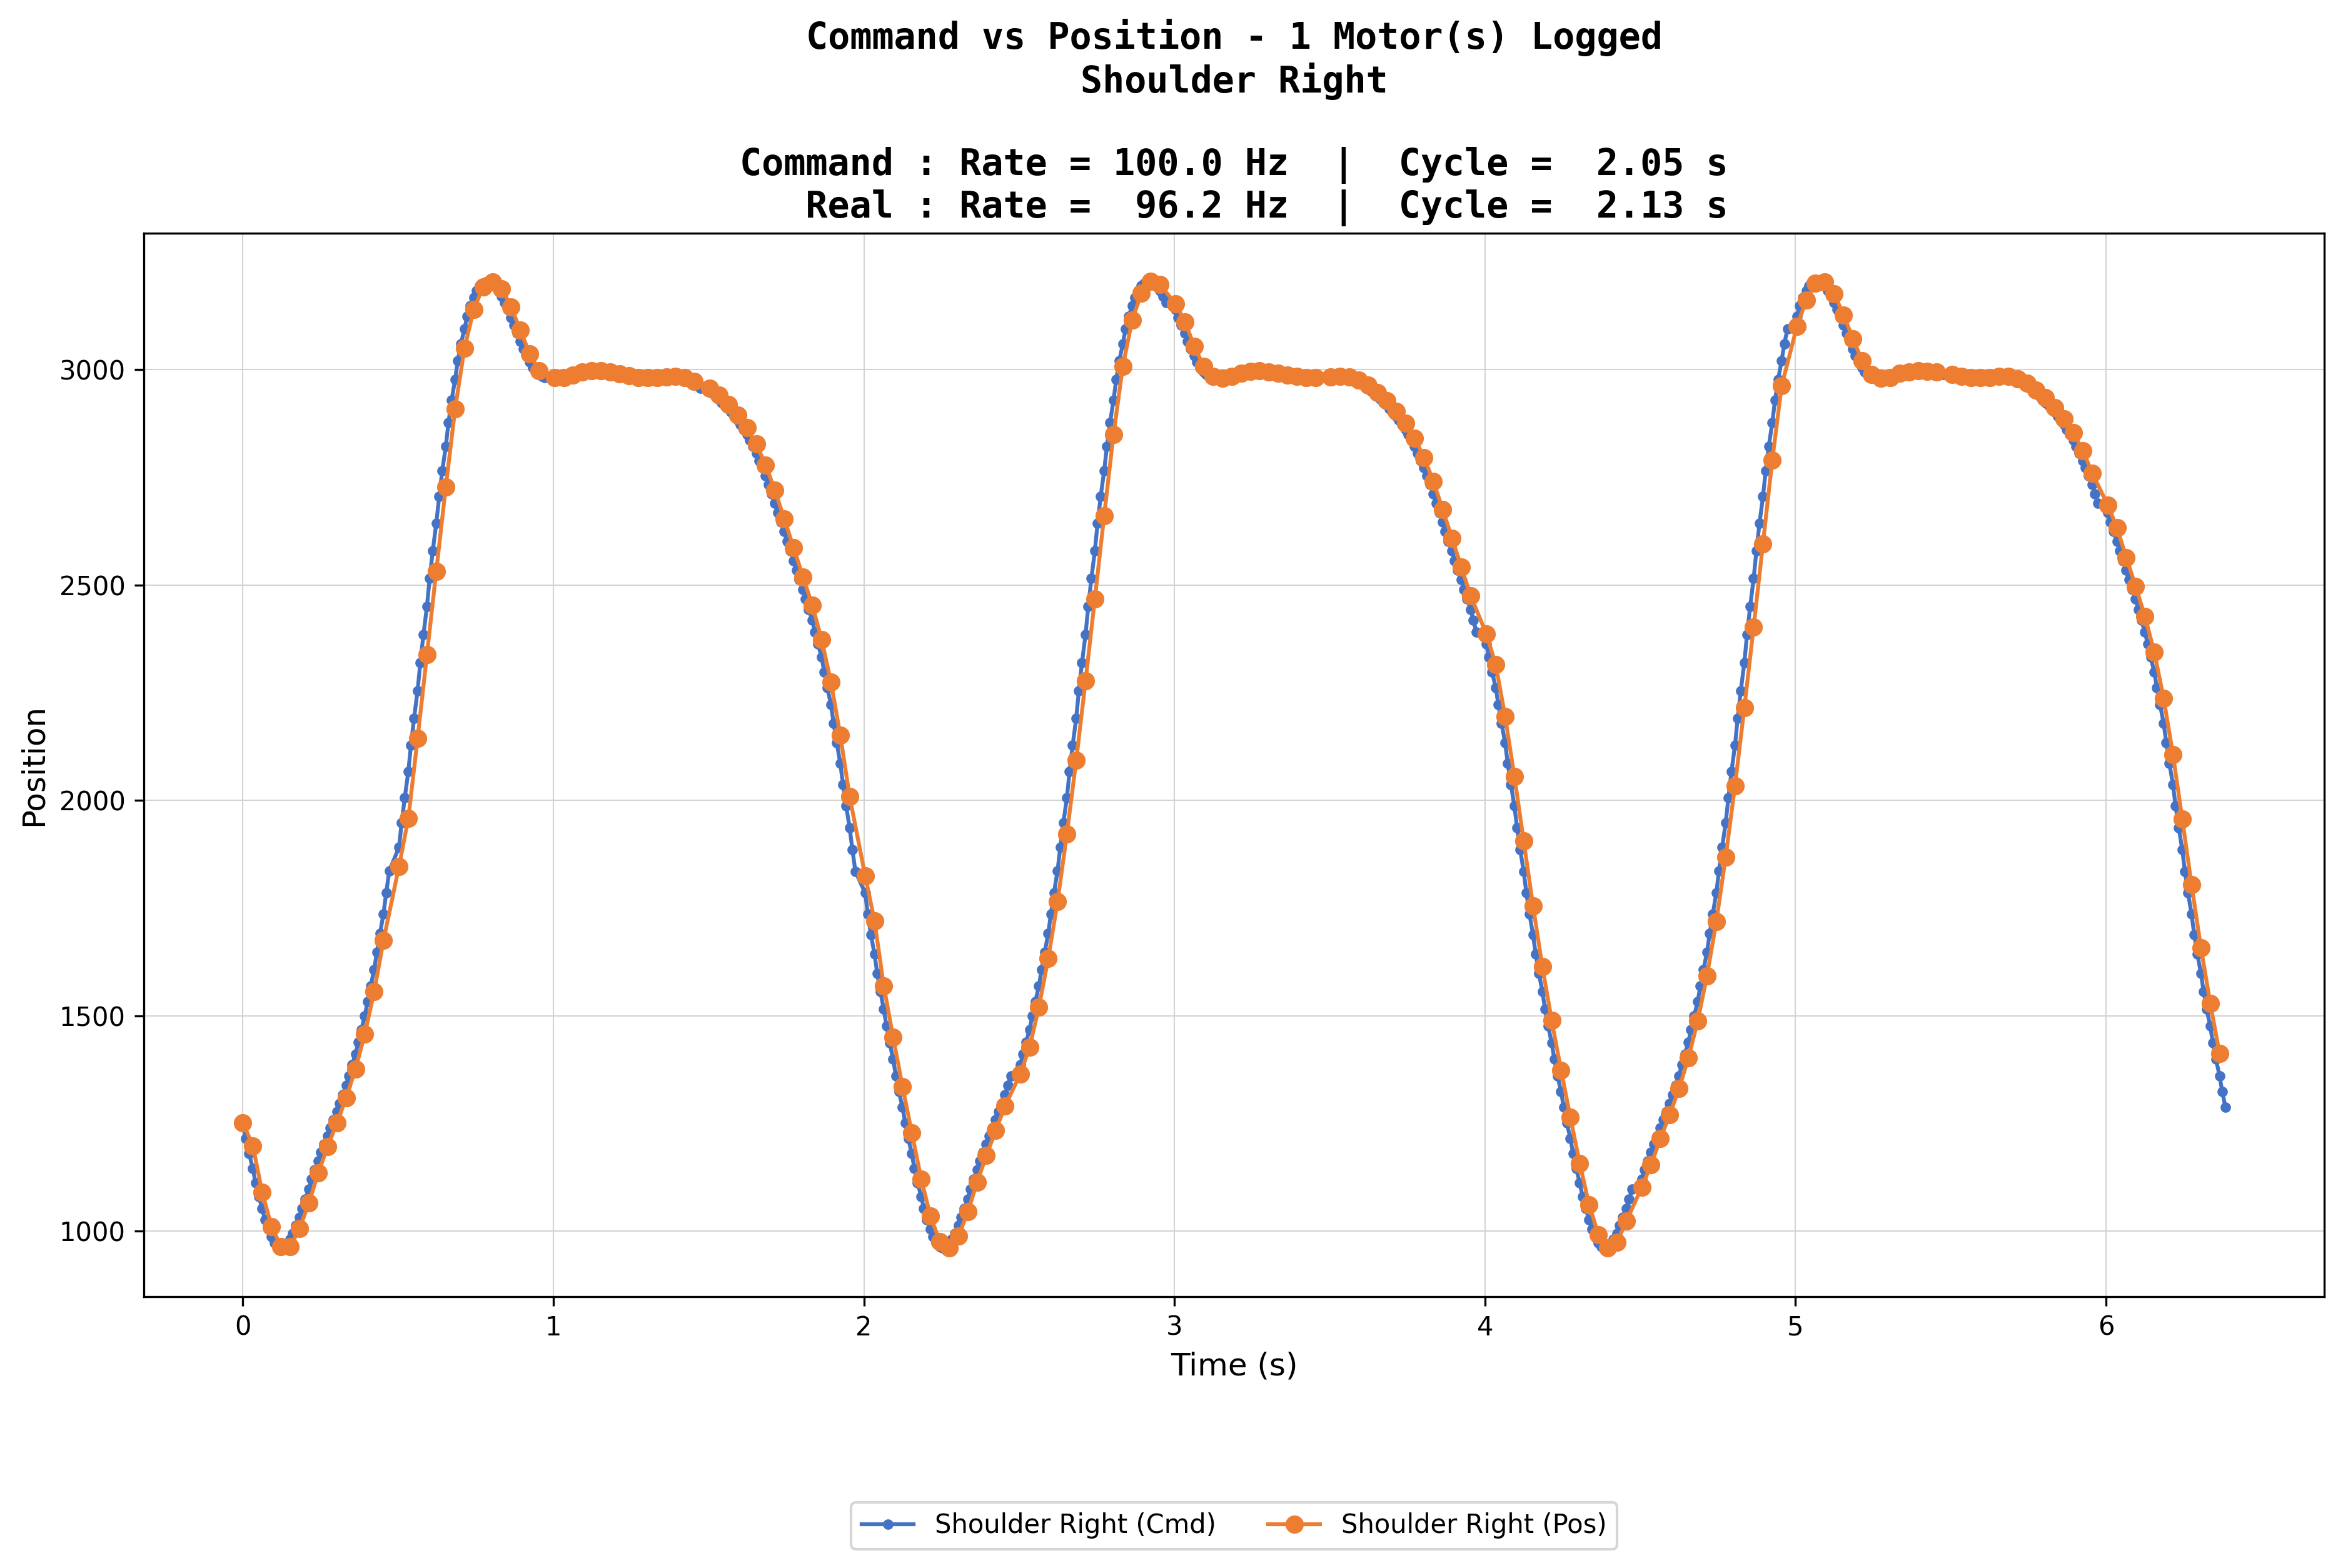
\includegraphics[width=\textwidth]{graphiques/log_100Hz_1mot.png}
        \caption{100\,Hz, $N = 1$ $\rightarrow$ 96.2 Hz.}
    \end{subfigure}
    \hfill
    \begin{subfigure}[b]{0.48\textwidth}
        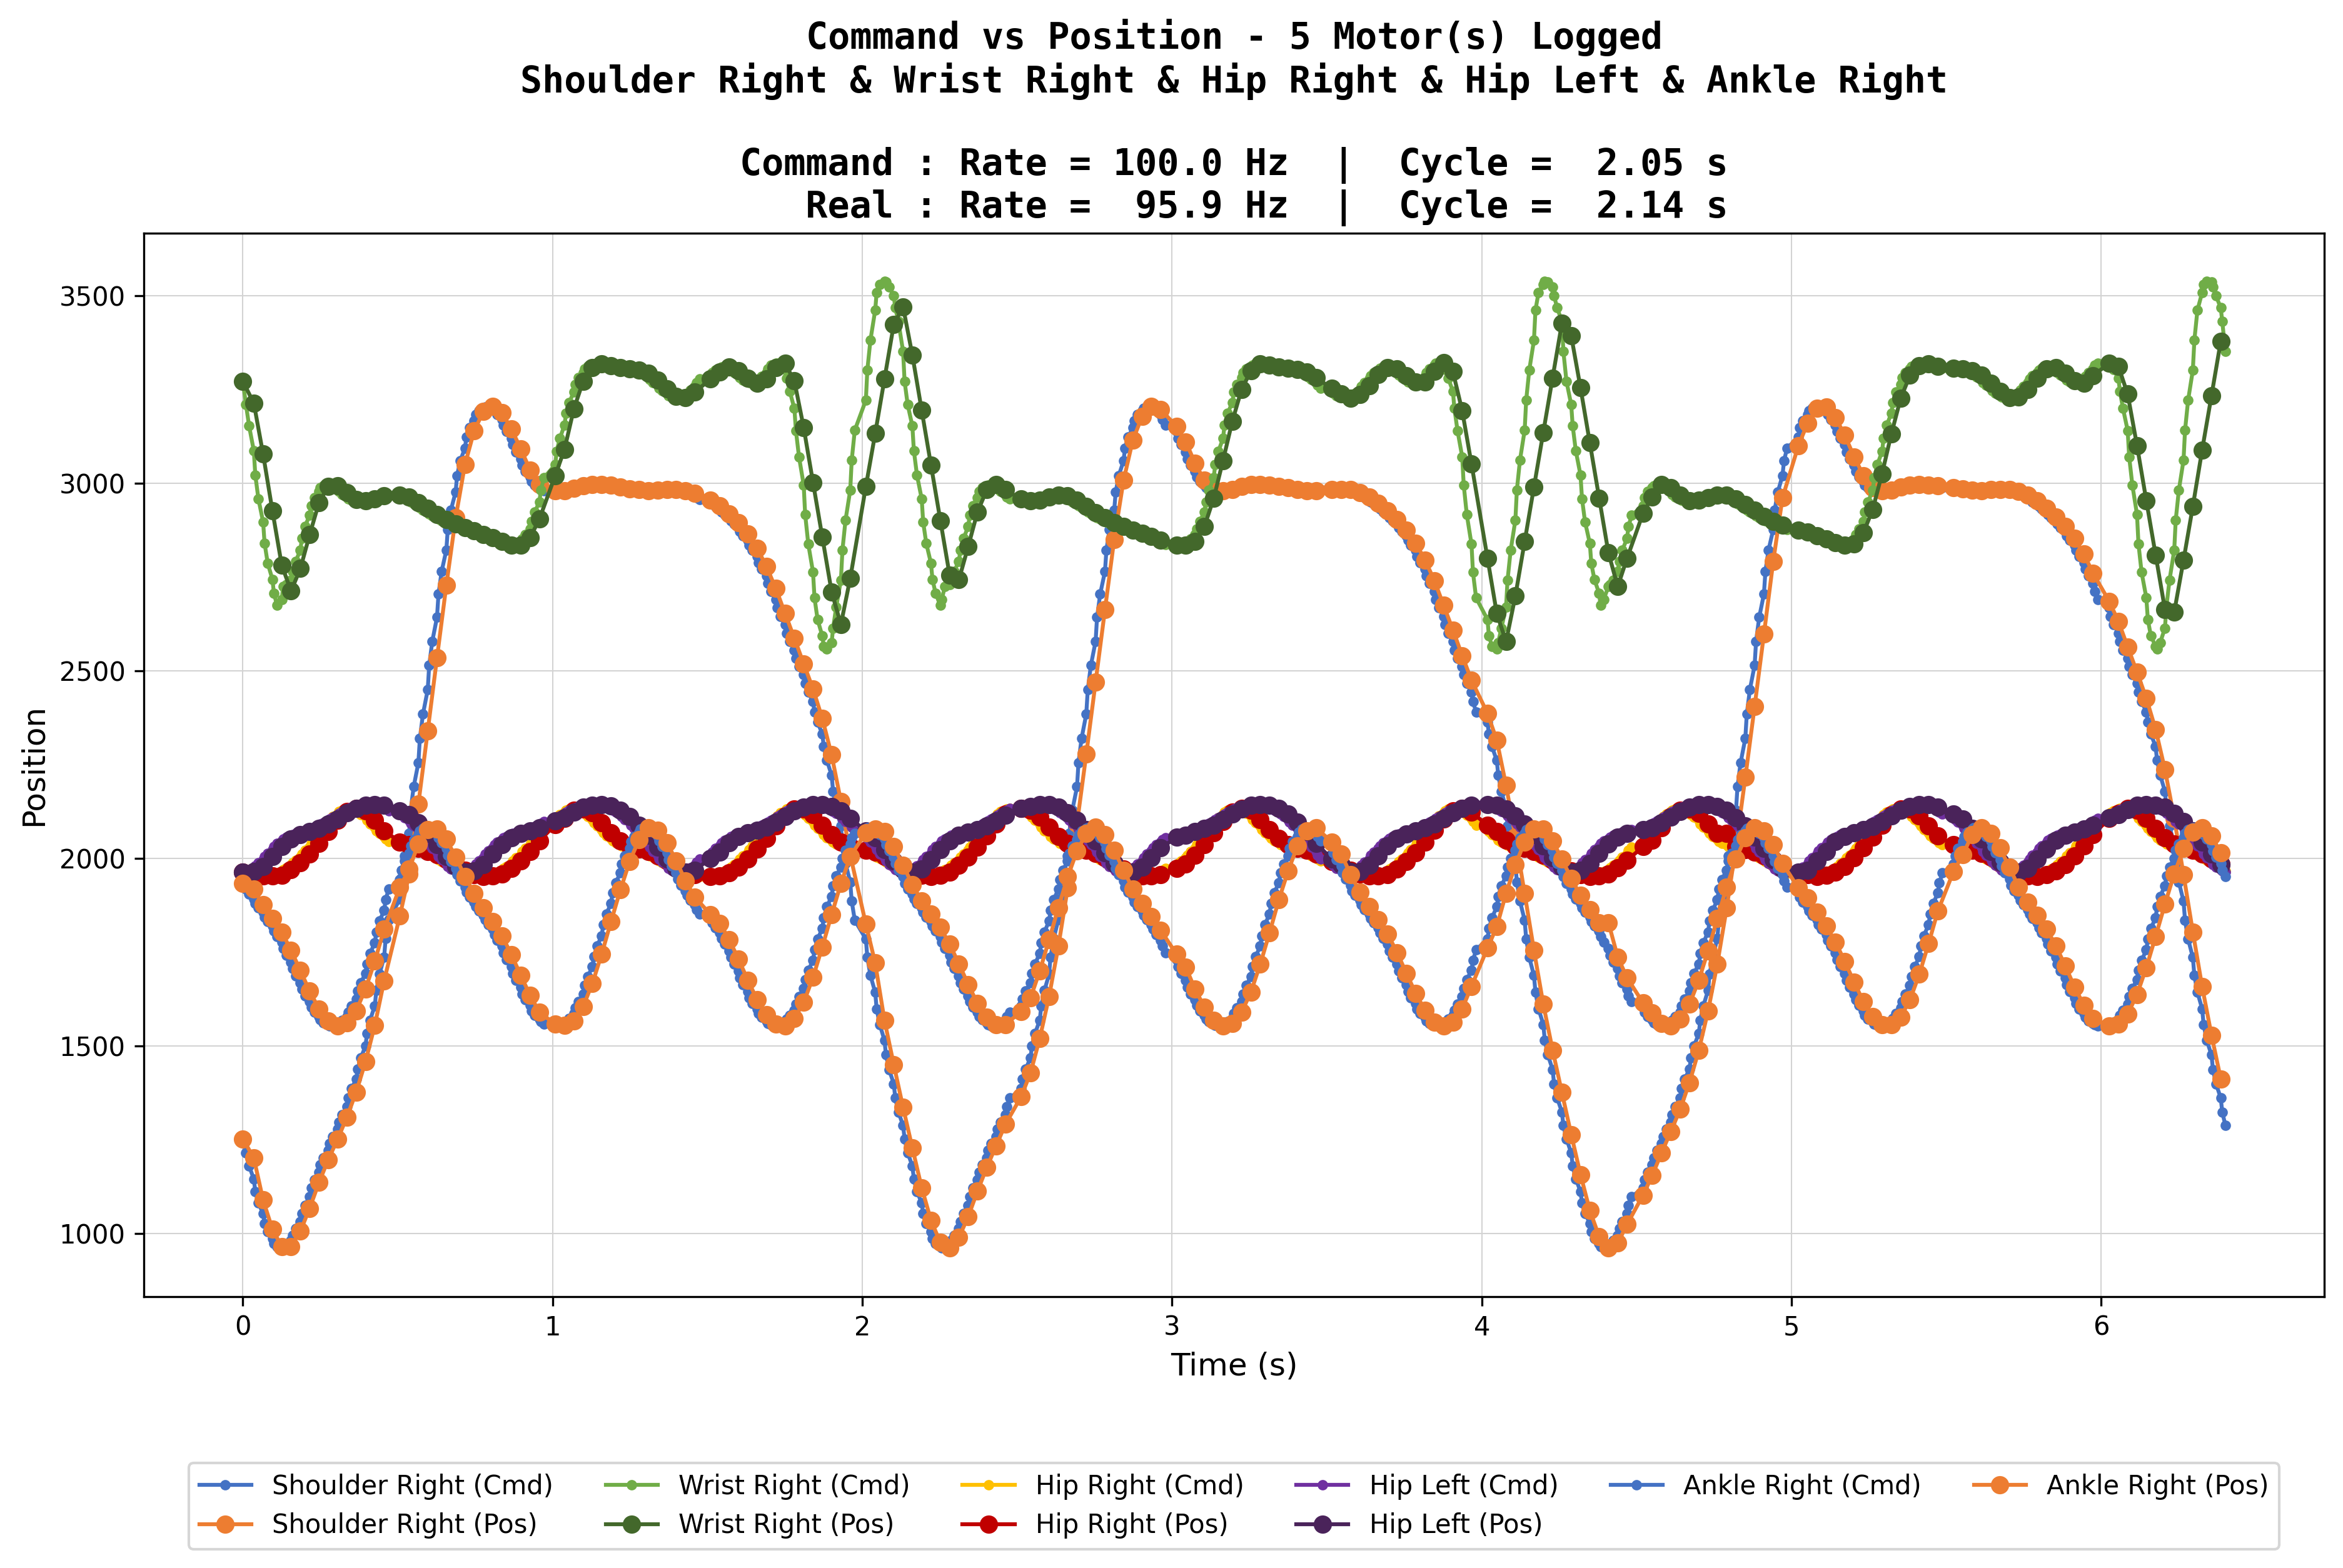
\includegraphics[width=\textwidth]{graphiques/log_100Hz_5mot.png}
        \caption{100\,Hz, $N = 5$ $\rightarrow$ 95.9 Hz.}
    \end{subfigure}
    \caption{Sweep of the number of logged motors at 100 Hz.}
    \label{fig:highfreq}
\end{figure}
\fi


\begin{figure}[H]
    \centering
    % Première ligne : 36 Hz
    \begin{subfigure}[b]{0.48\textwidth}
        \centering
        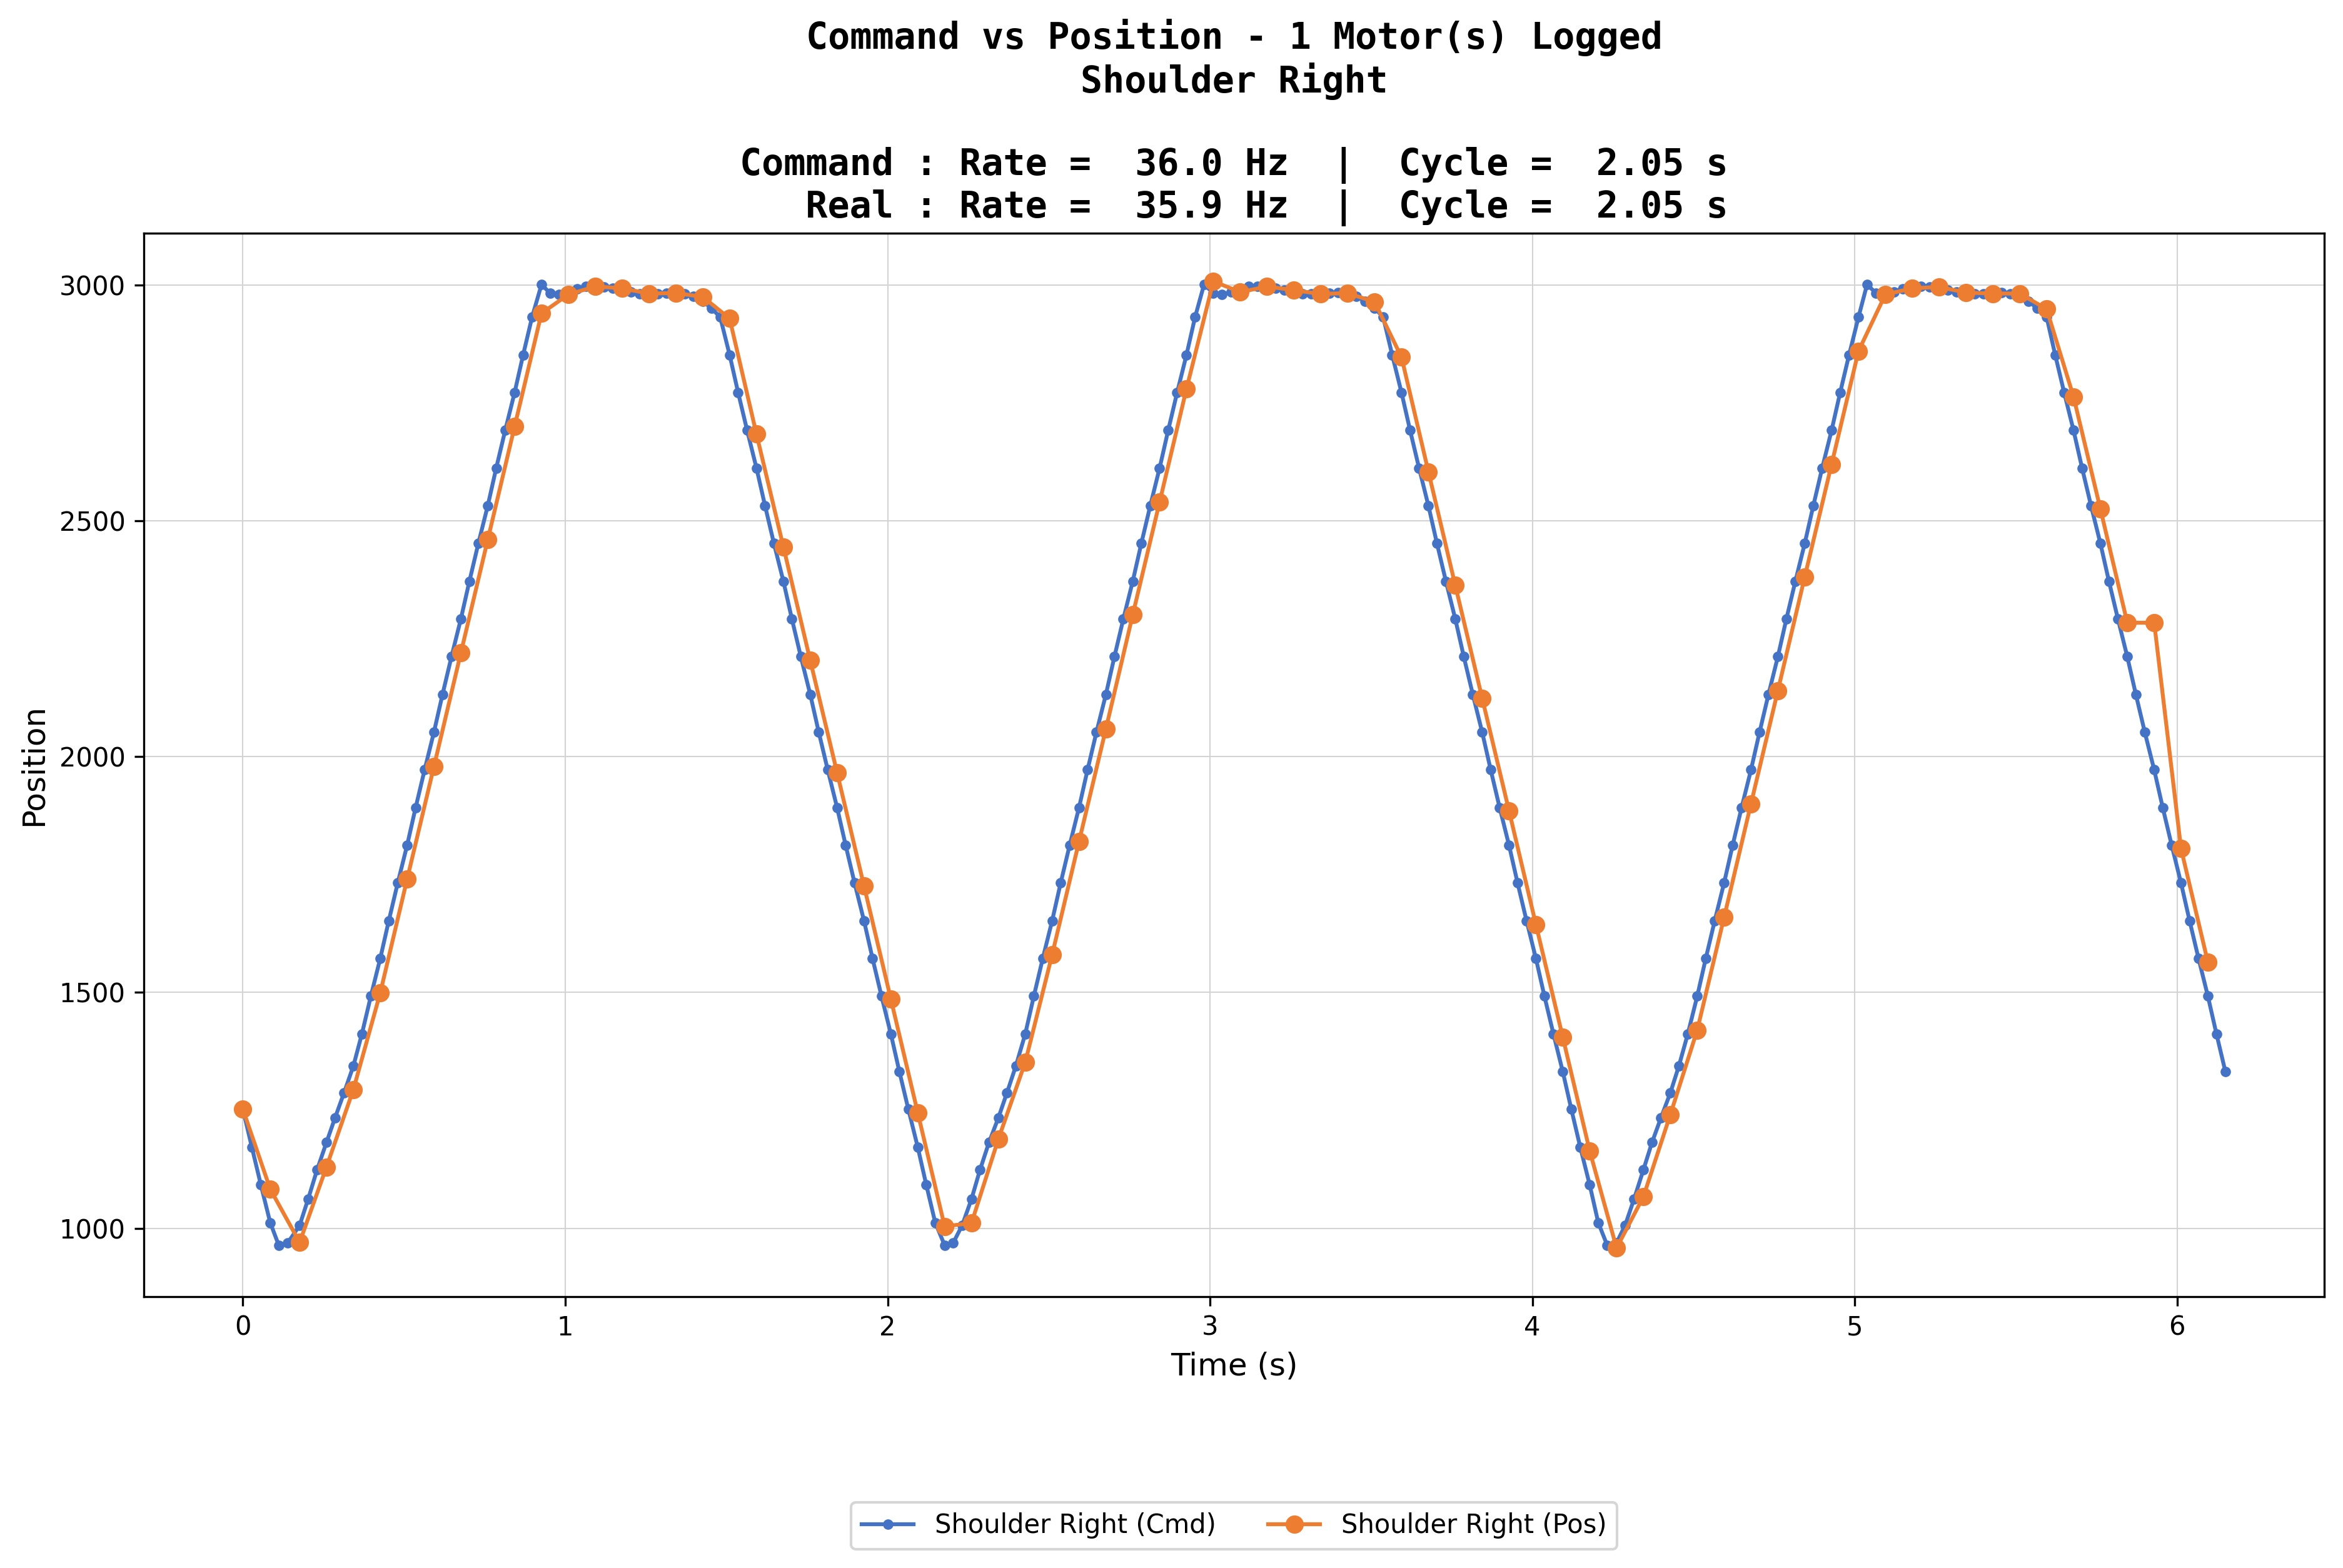
\includegraphics[width=\textwidth]{graphiques/log_36Hz_1mot.png}
        \caption{36\,Hz, $N = 1$ $\rightarrow$ 35.9 Hz.}
        \label{fig:log_36Hz_1mot}
    \end{subfigure}
    \hfill
    \begin{subfigure}[b]{0.48\textwidth}
        \centering
        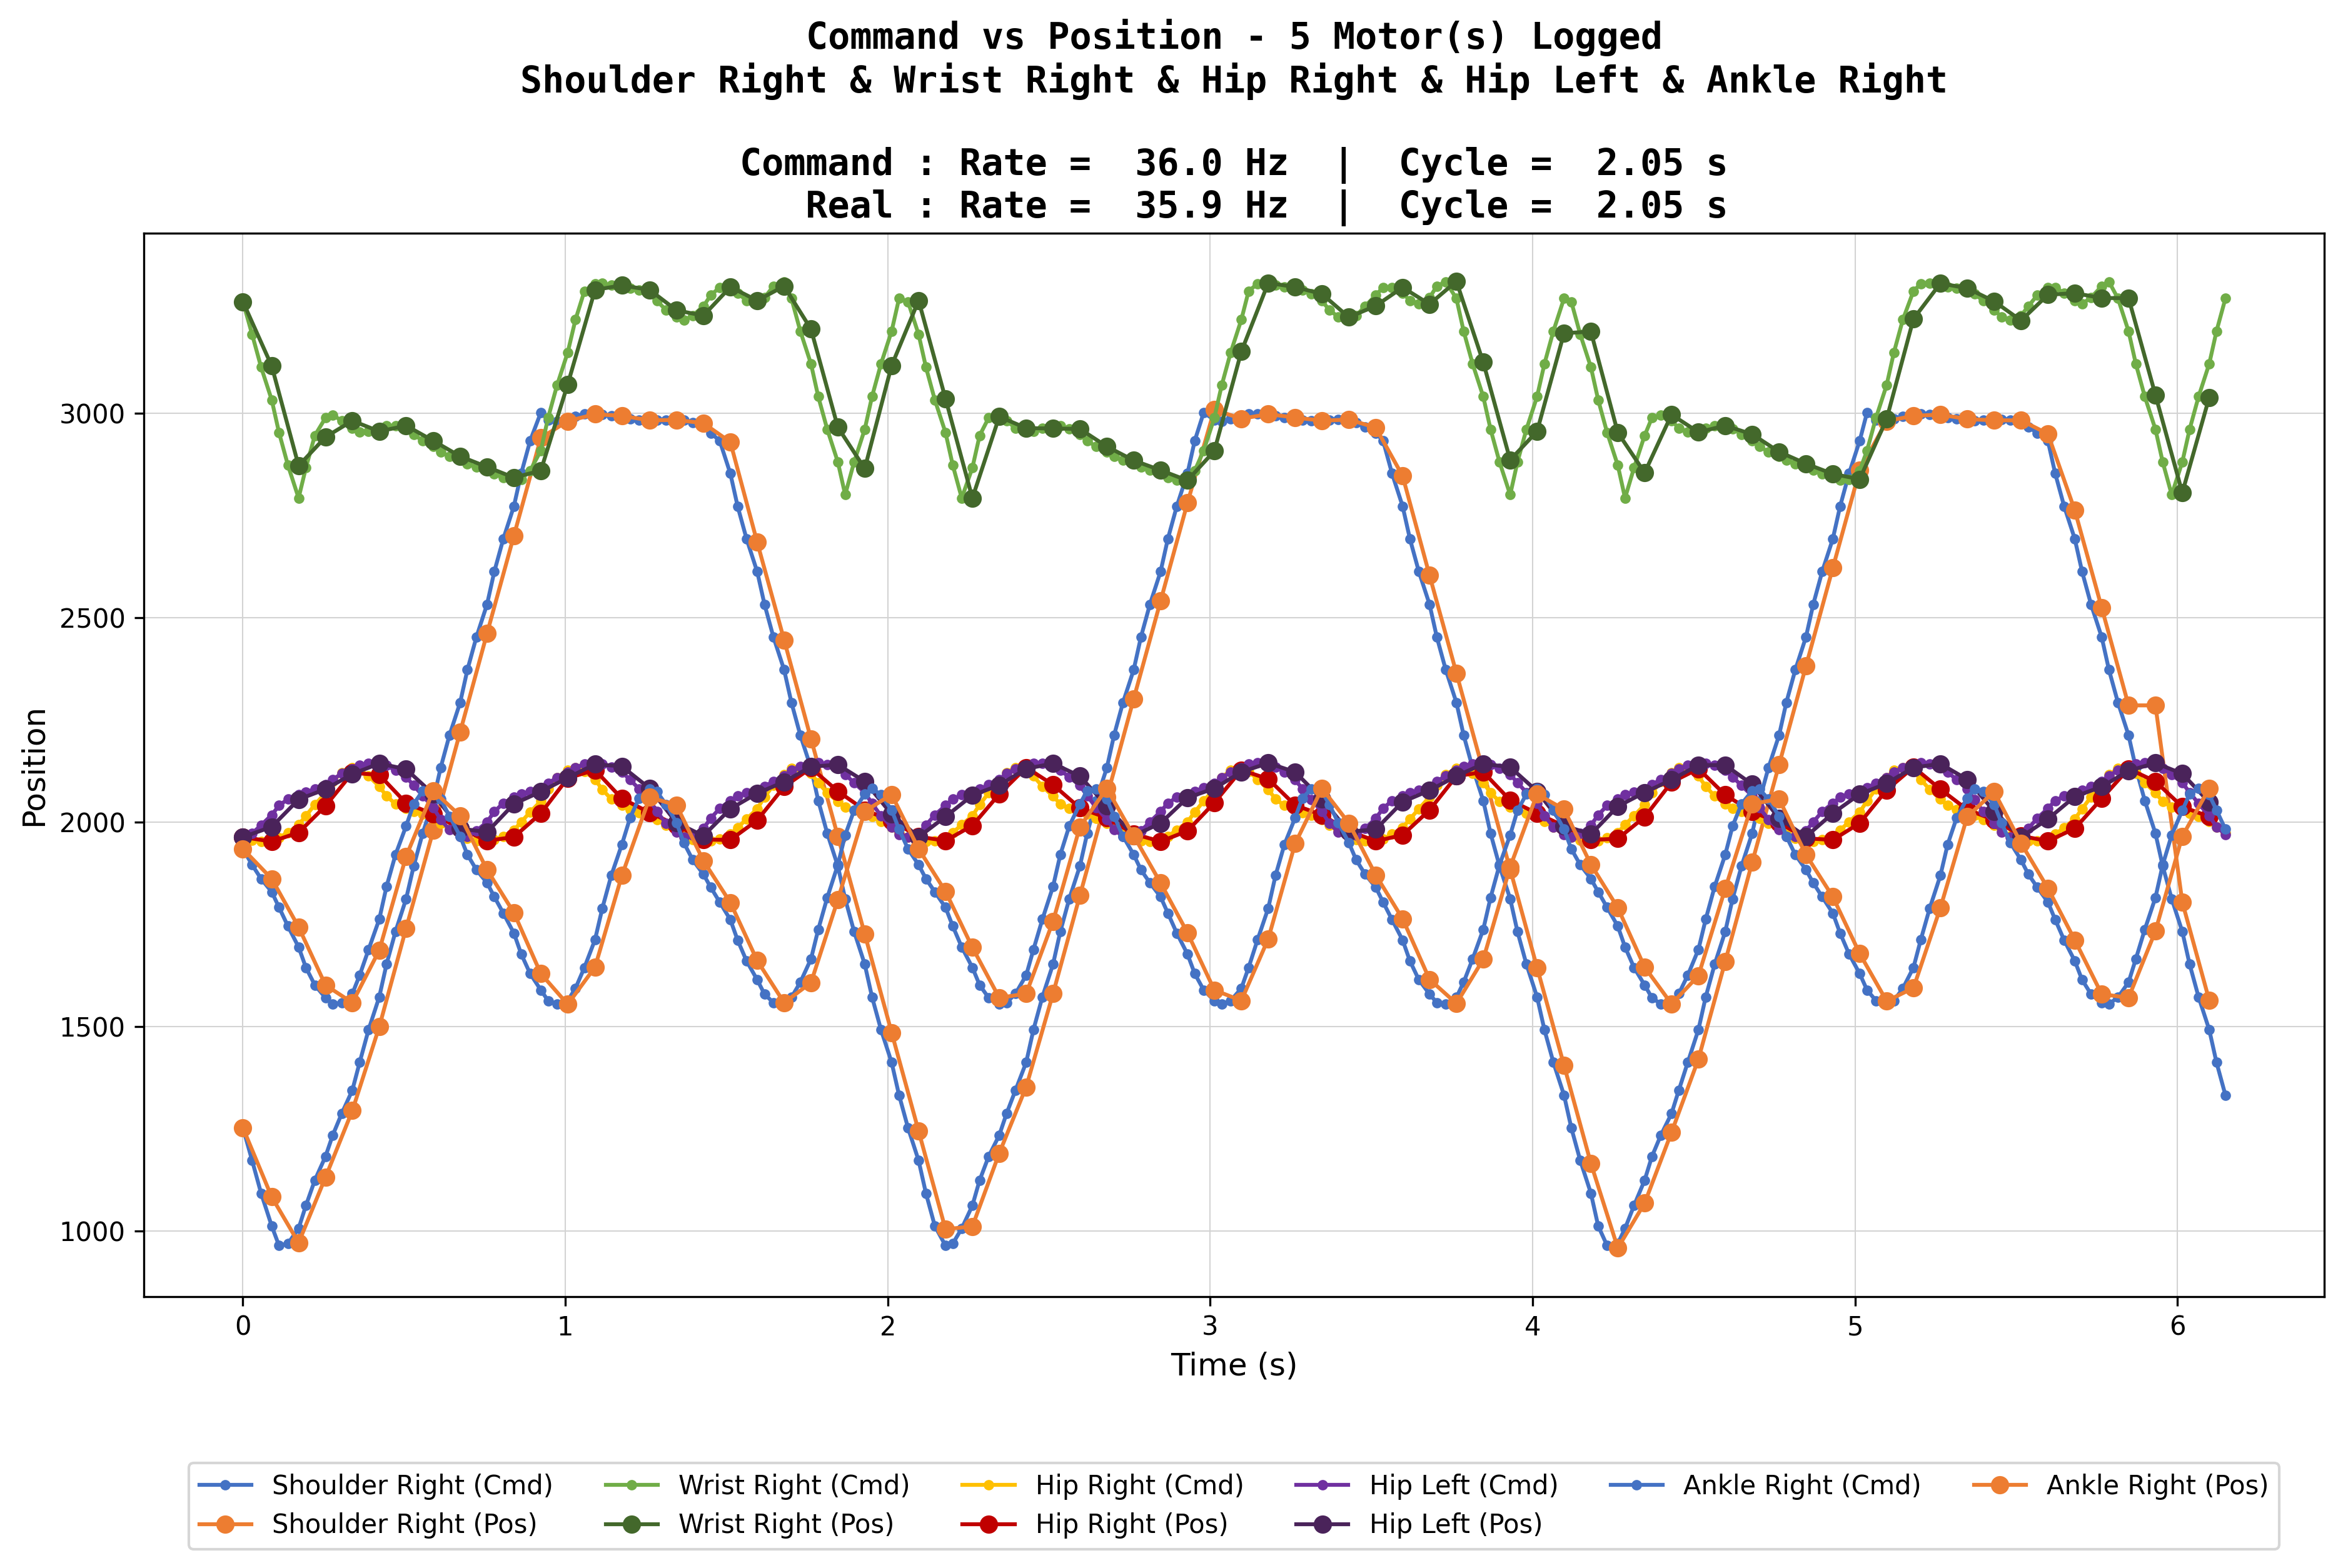
\includegraphics[width=\textwidth]{graphiques/log_36Hz_5mot.png}
        \caption{36\,Hz, $N = 5$ $\rightarrow$ 35.9 Hz.}
        \label{fig:log_36Hz_5mot}
    \end{subfigure}
    
    \vspace{0.3cm} % Espace vertical entre les lignes de graphiques

    % Deuxième ligne : 72 Hz
    \begin{subfigure}[b]{0.48\textwidth}
        \centering
        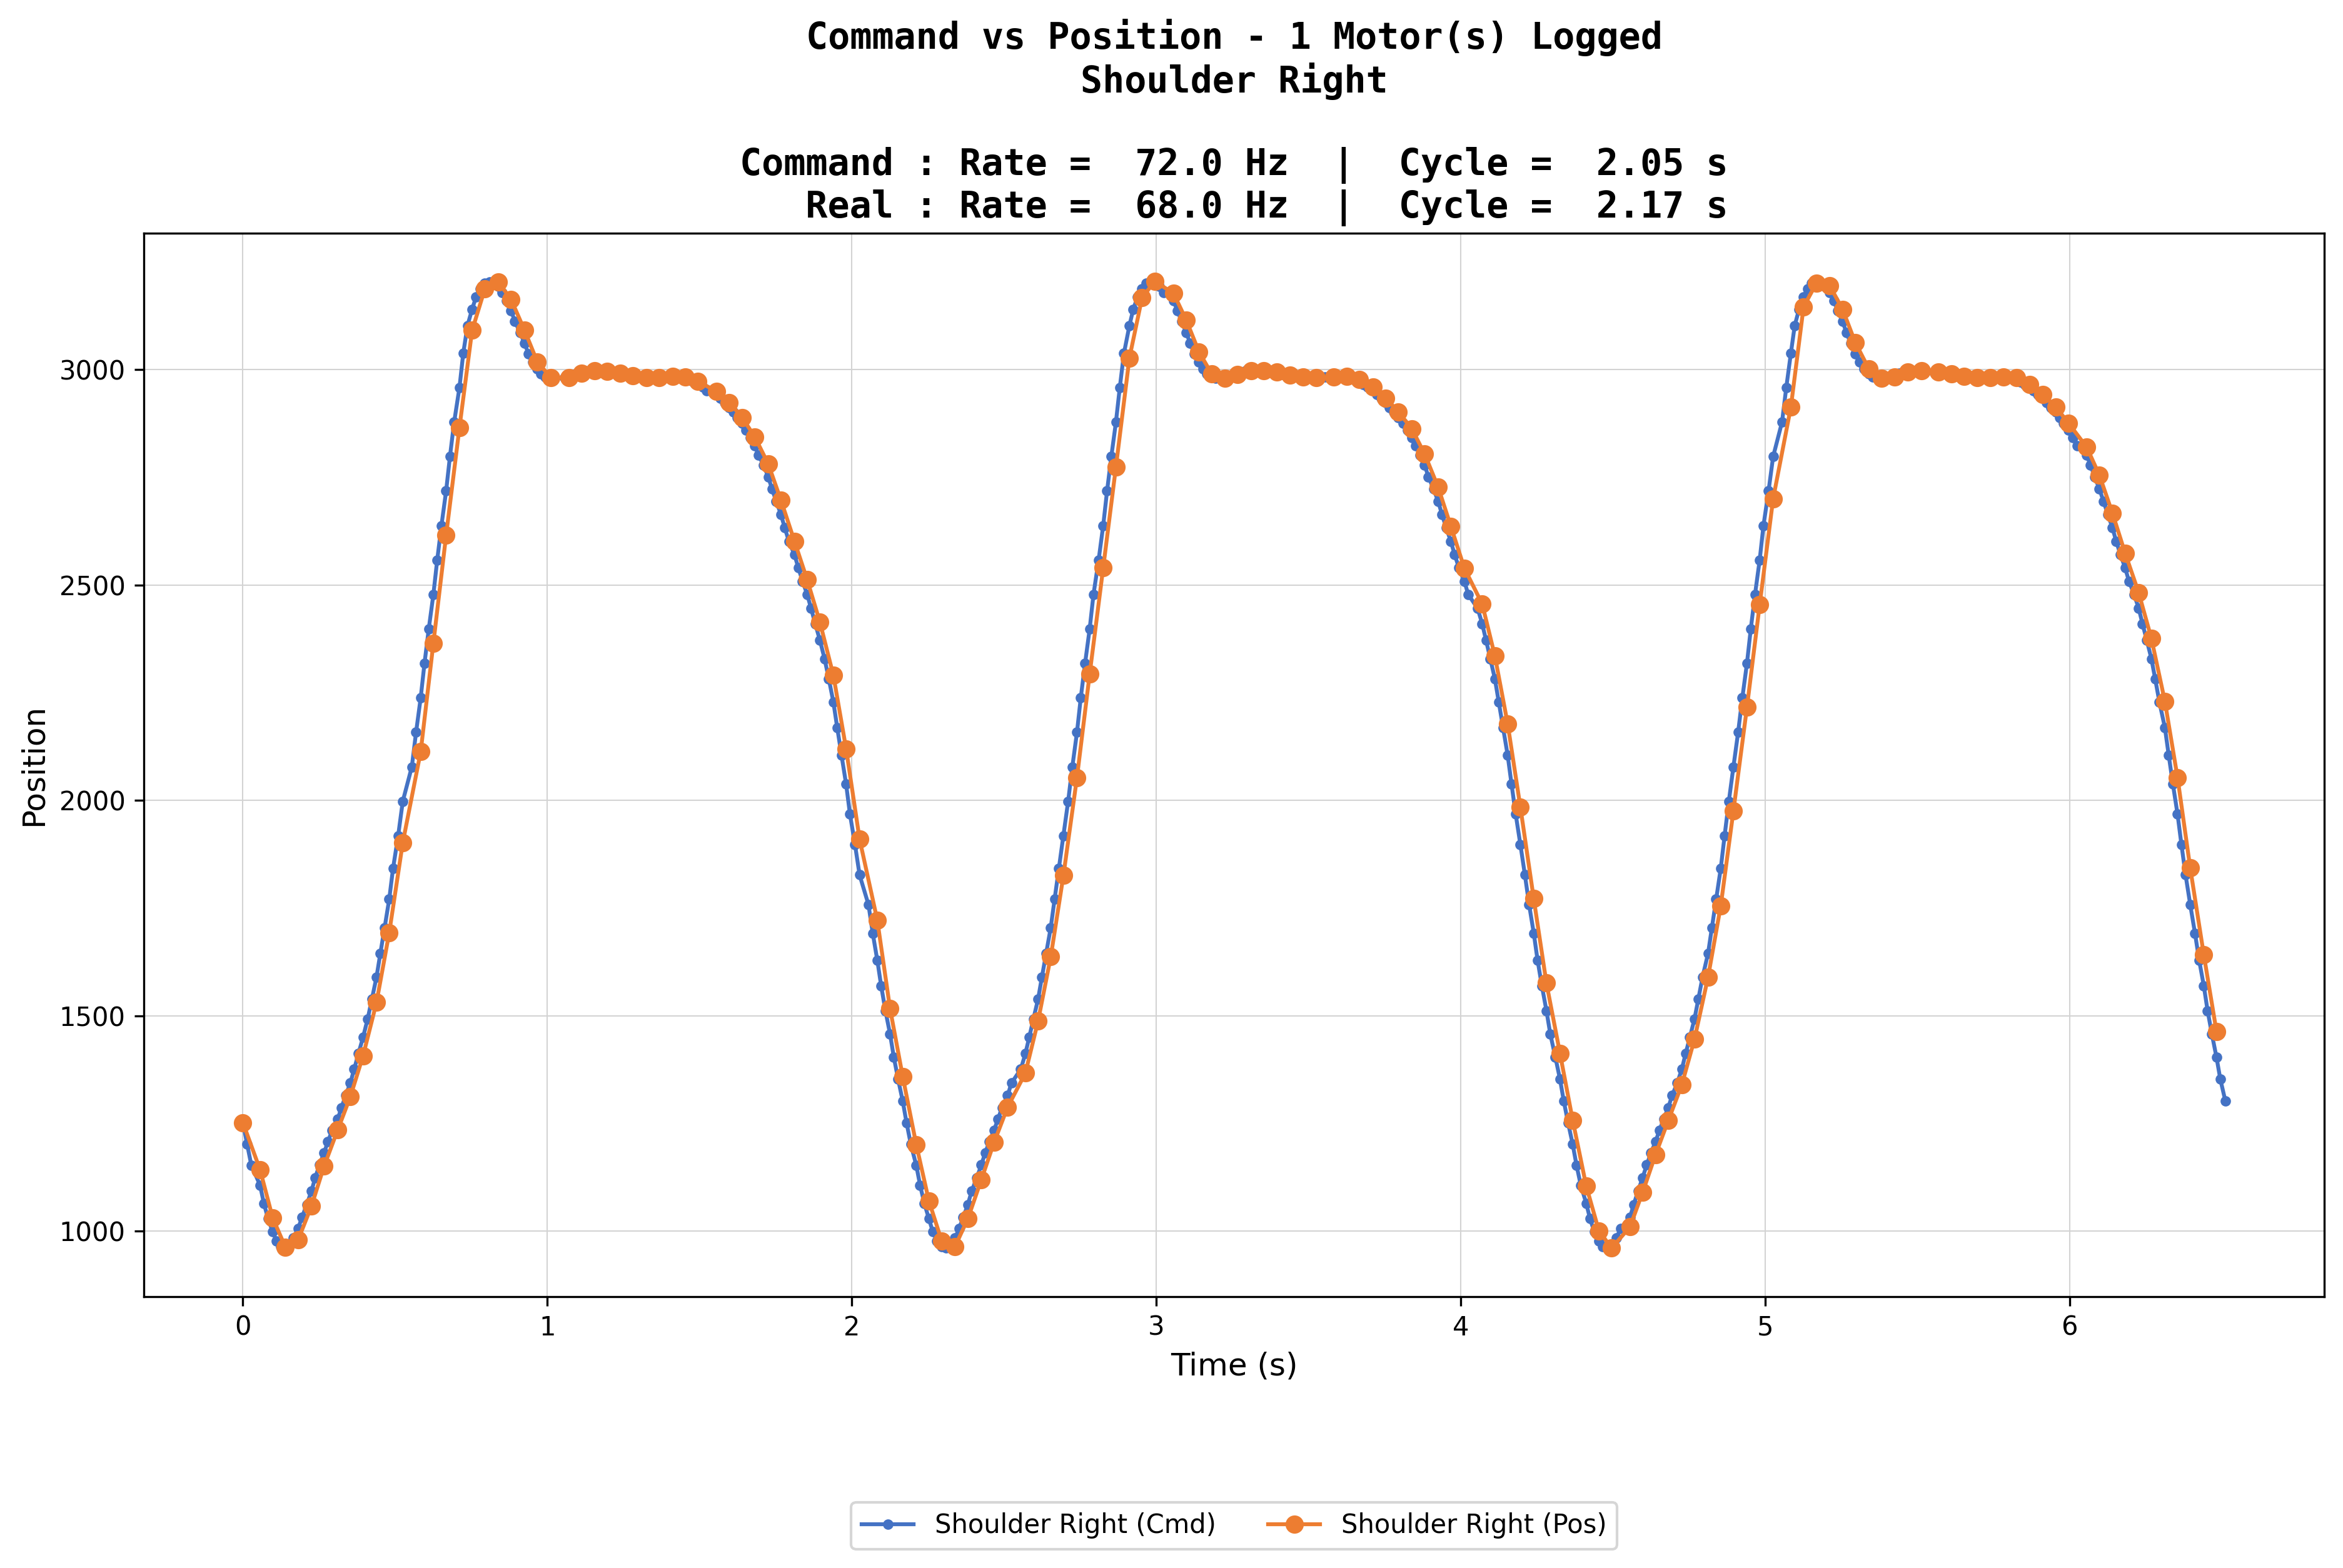
\includegraphics[width=\textwidth]{graphiques/log_72Hz_1mot.png}
        \caption{72\,Hz, $N = 1$ $\rightarrow$ 68.0 Hz.}
        \label{fig:log_72Hz_1mot}
    \end{subfigure}
    \hfill
    \begin{subfigure}[b]{0.48\textwidth}
        \centering
        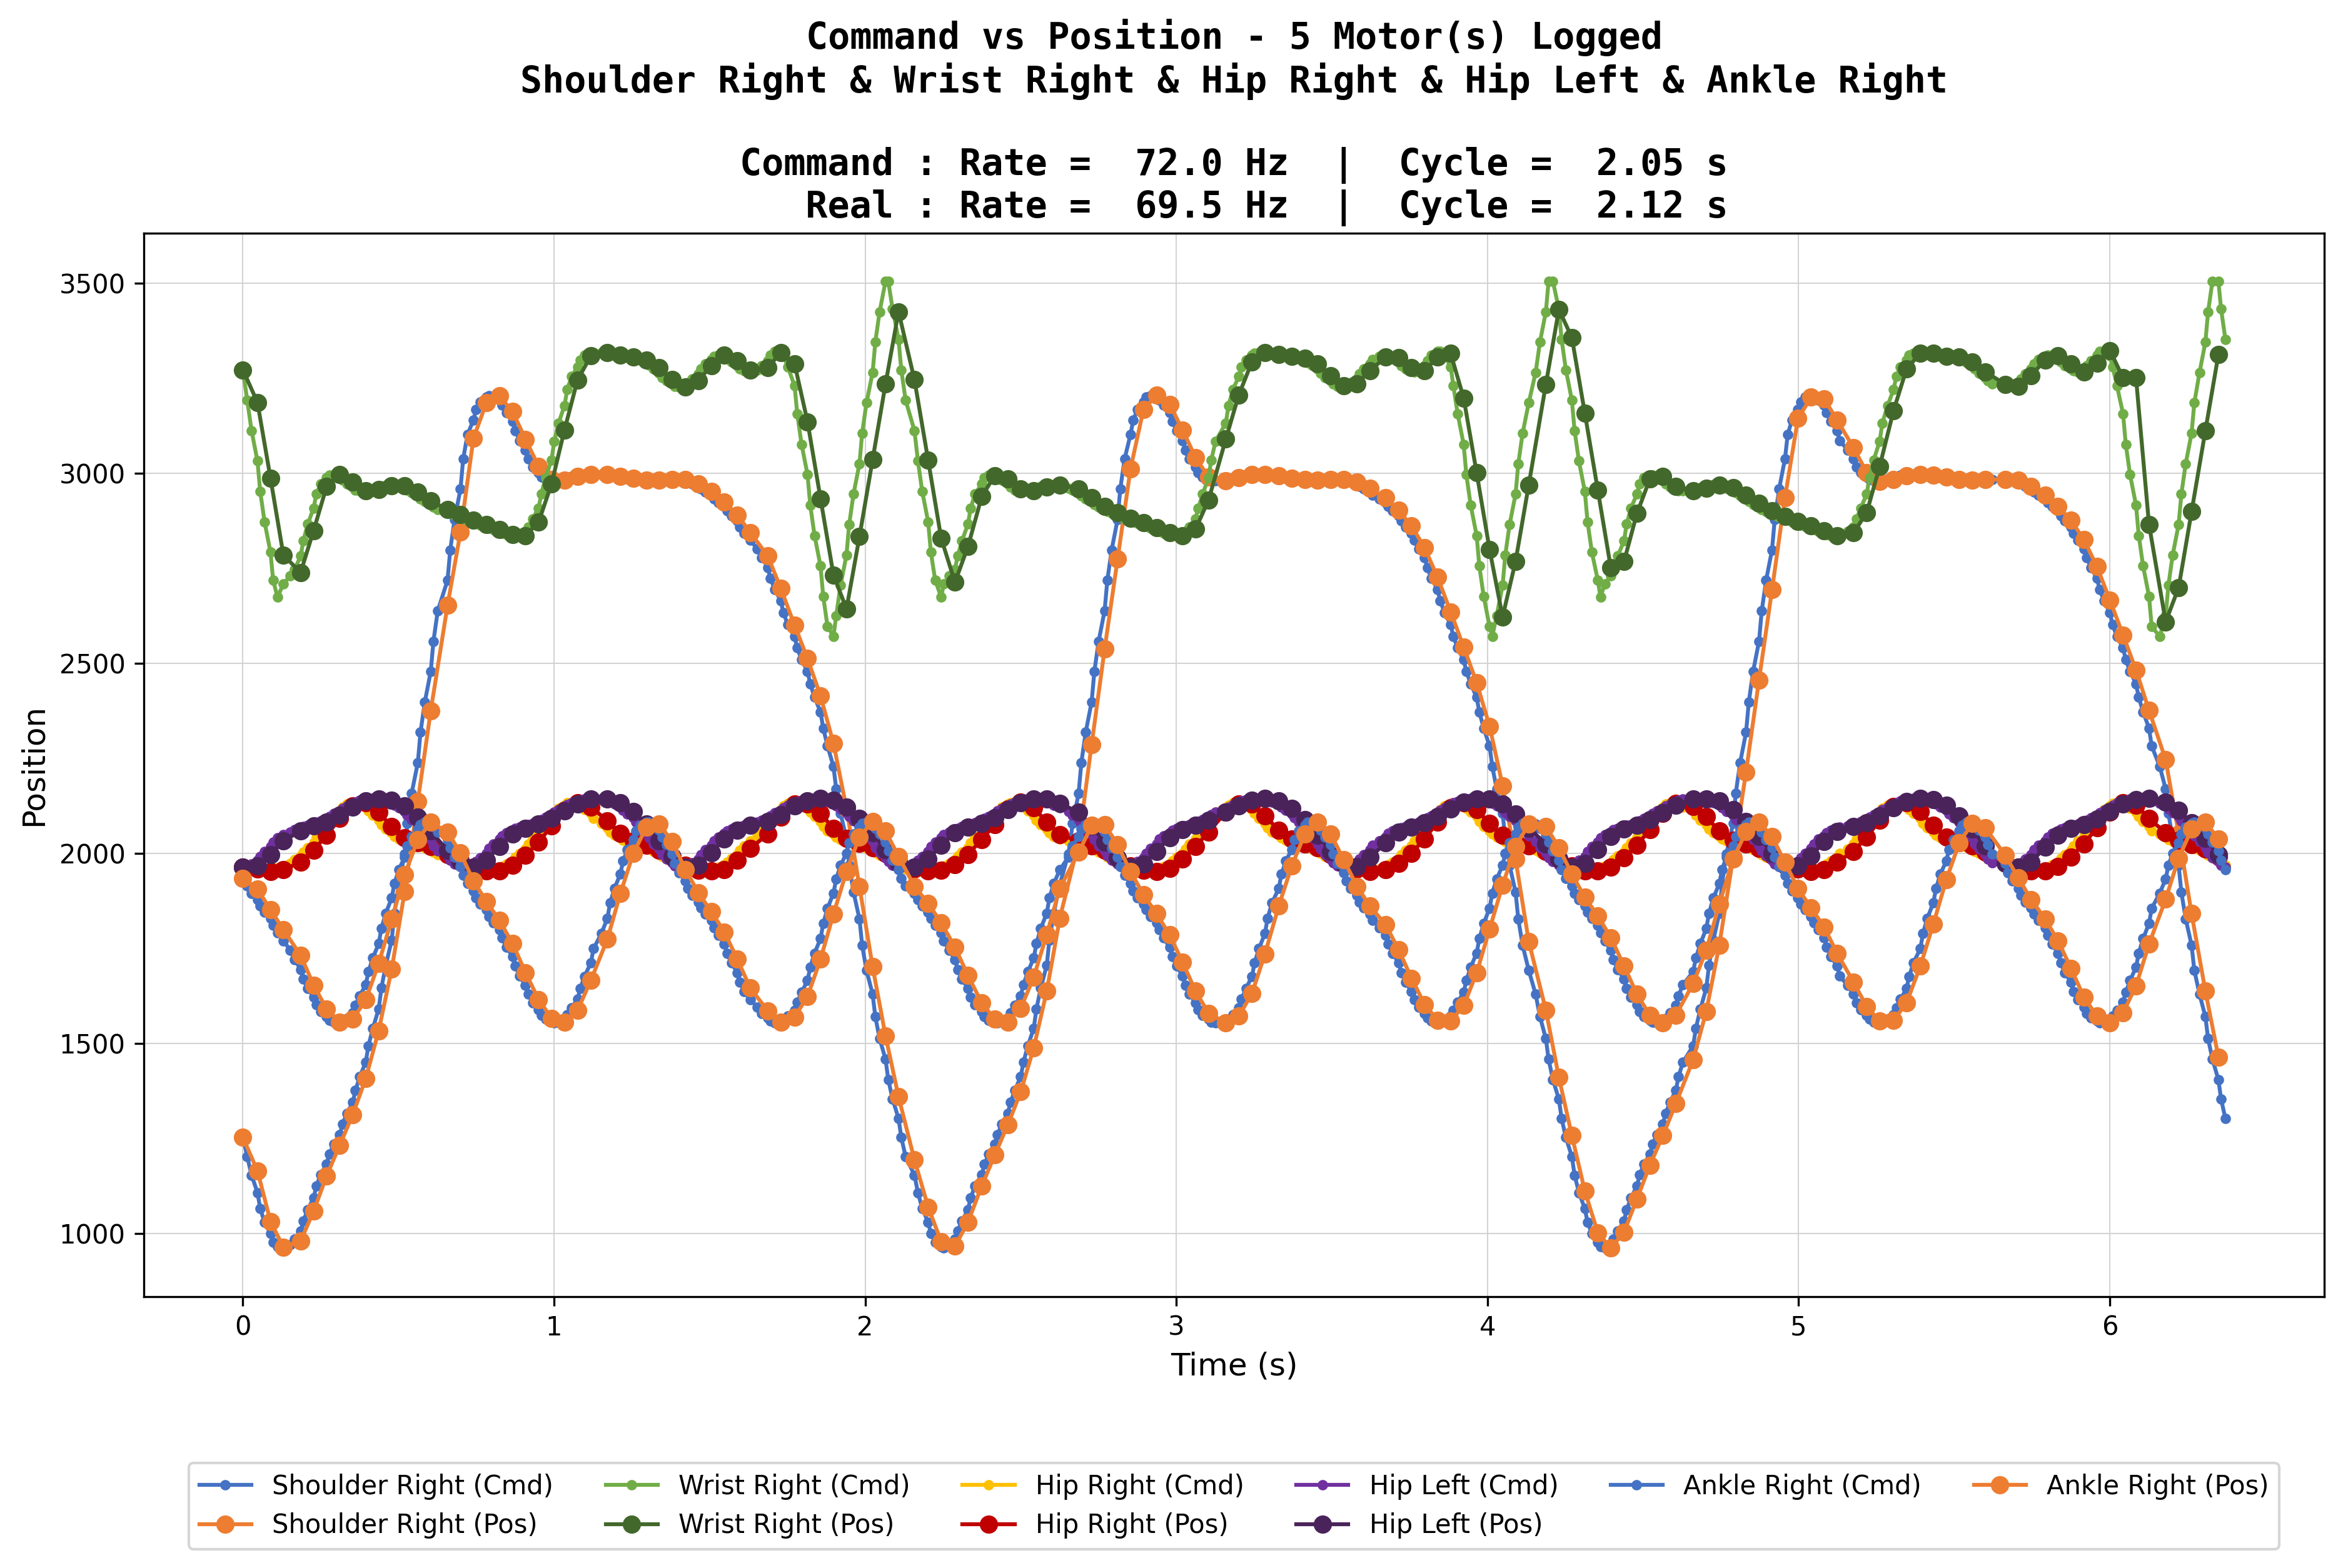
\includegraphics[width=\textwidth]{graphiques/log_72Hz_5mot.png}
        \caption{72\,Hz, $N = 5$ $\rightarrow$ 69.5 Hz.}
        \label{fig:log_72Hz_5mot}
    \end{subfigure}

    \vspace{0.3cm}

    % Troisième ligne : 100 Hz
    \begin{subfigure}[b]{0.48\textwidth}
        \centering
        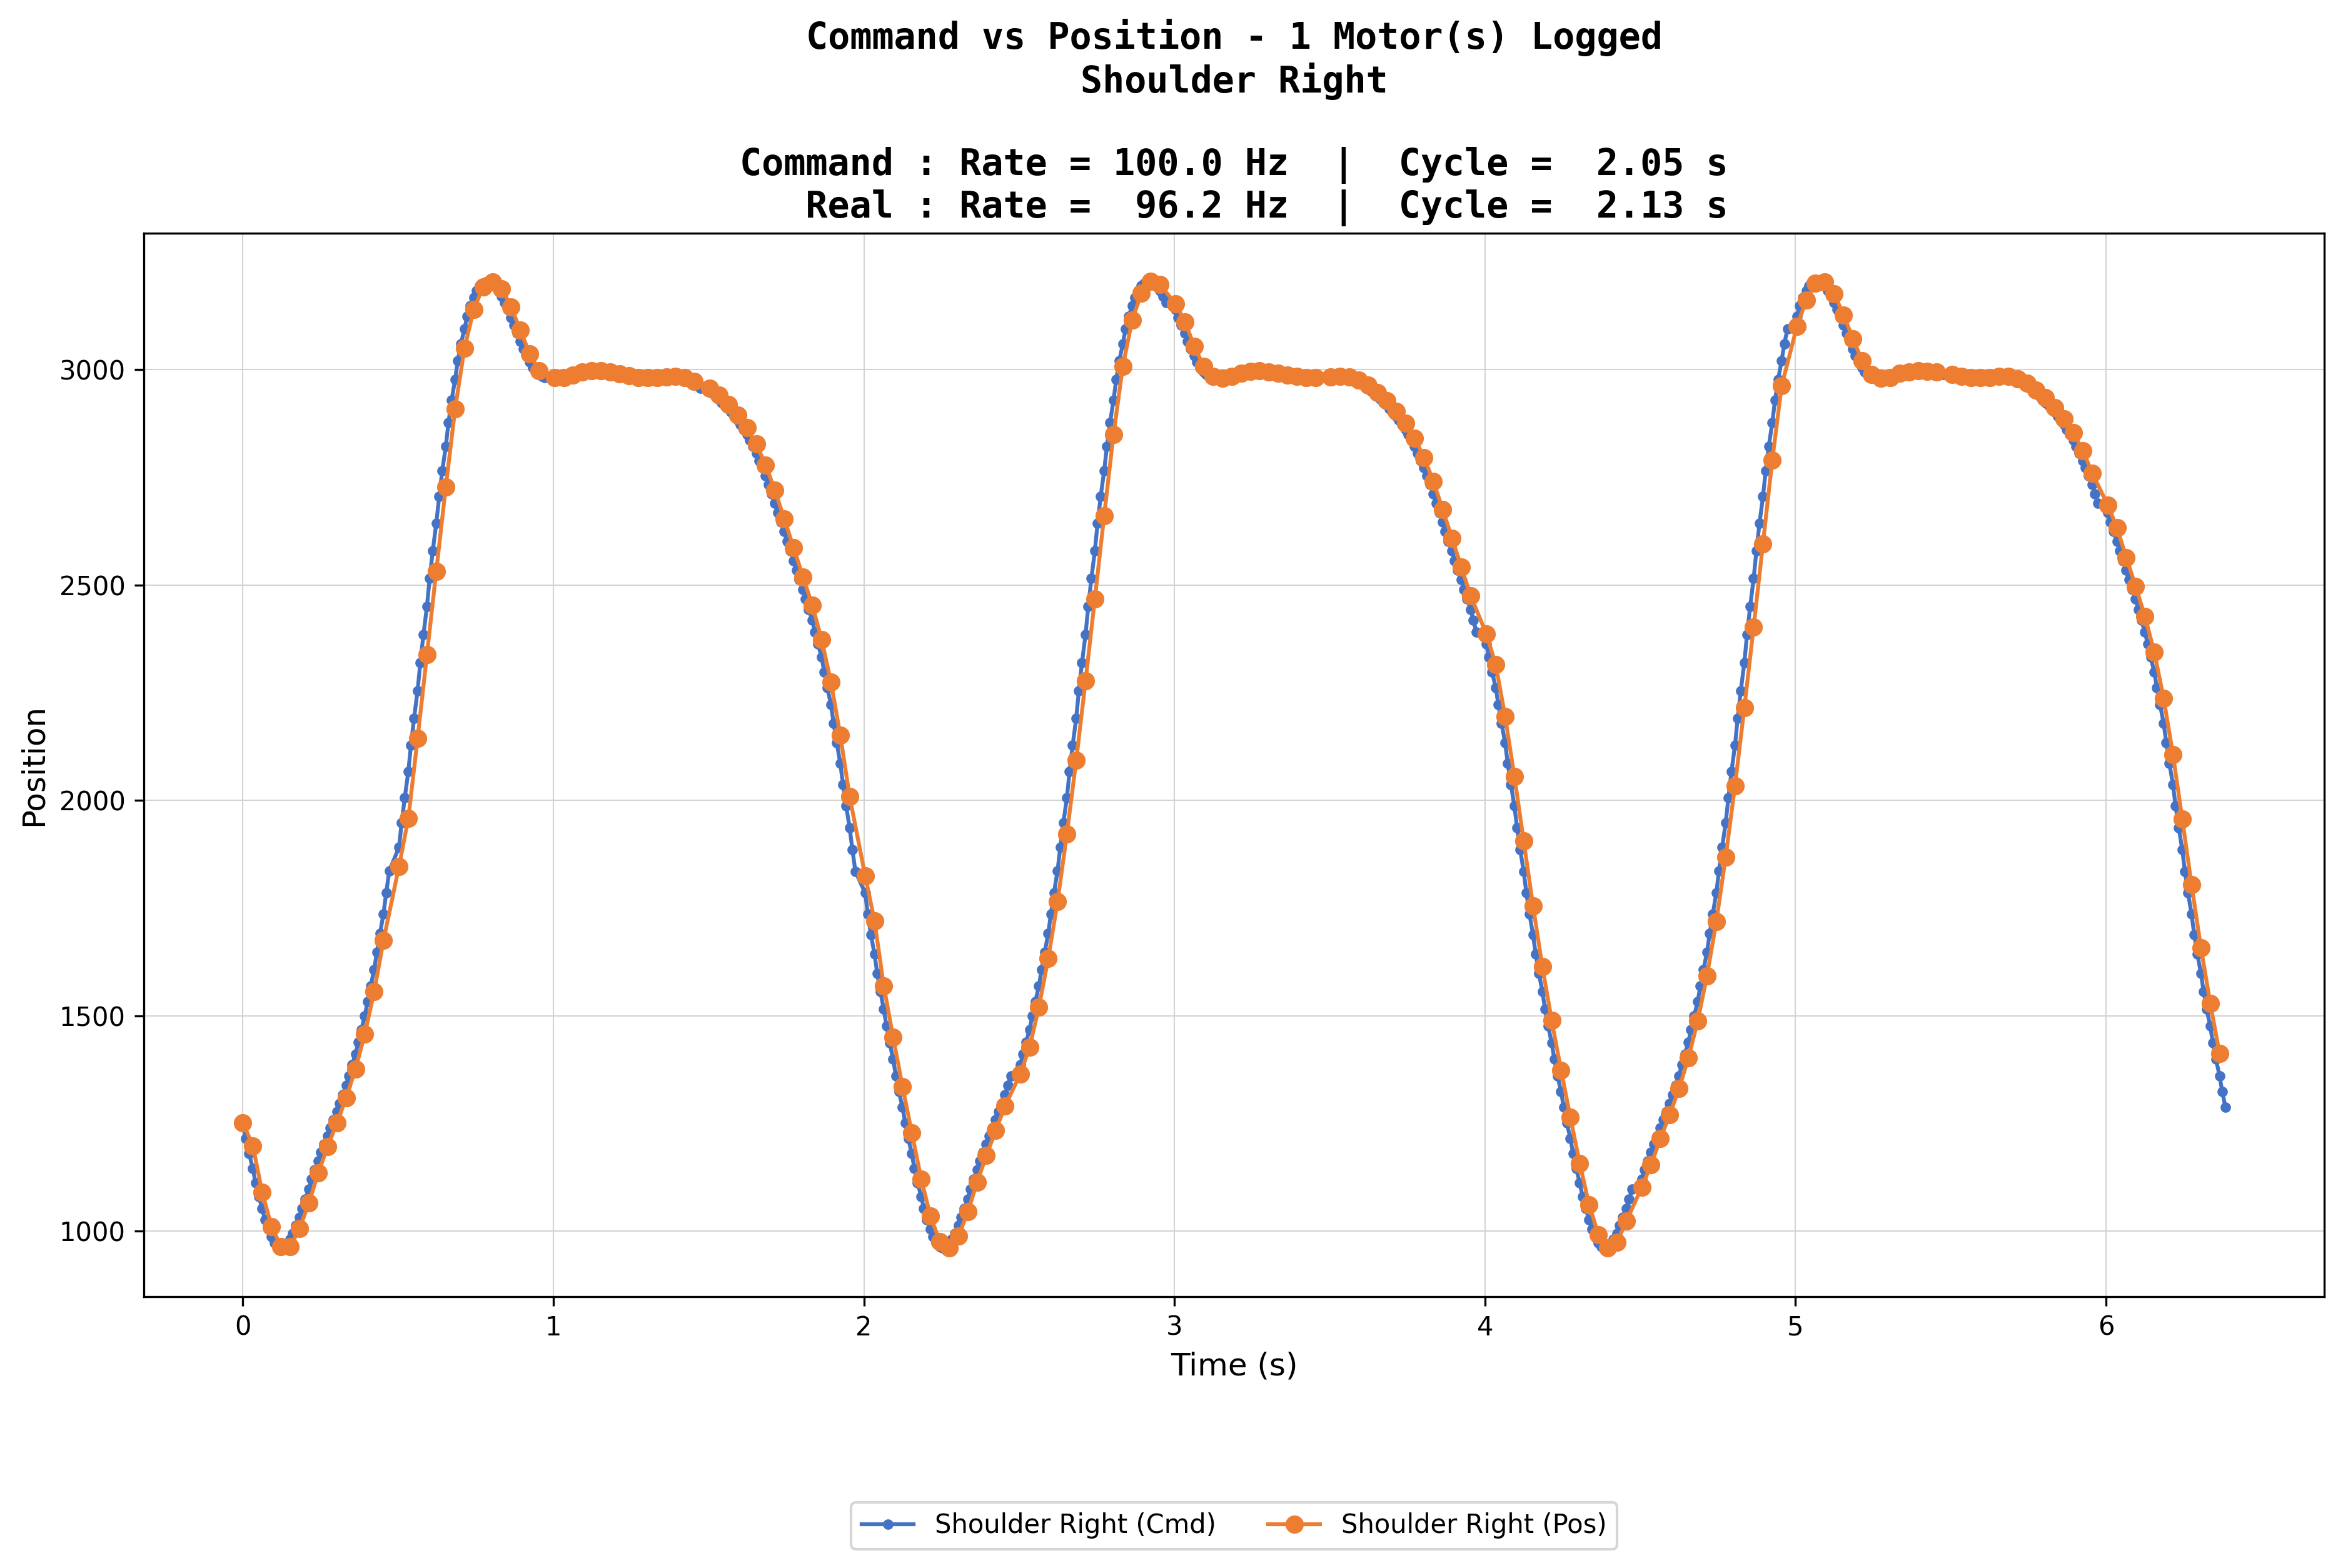
\includegraphics[width=\textwidth]{graphiques/log_100Hz_1mot.png}
        \caption{100\,Hz, $N = 1$ $\rightarrow$ 96.2 Hz.}
        \label{fig:log_100Hz_1mot}
    \end{subfigure}
    \hfill
    \begin{subfigure}[b]{0.48\textwidth}
        \centering
        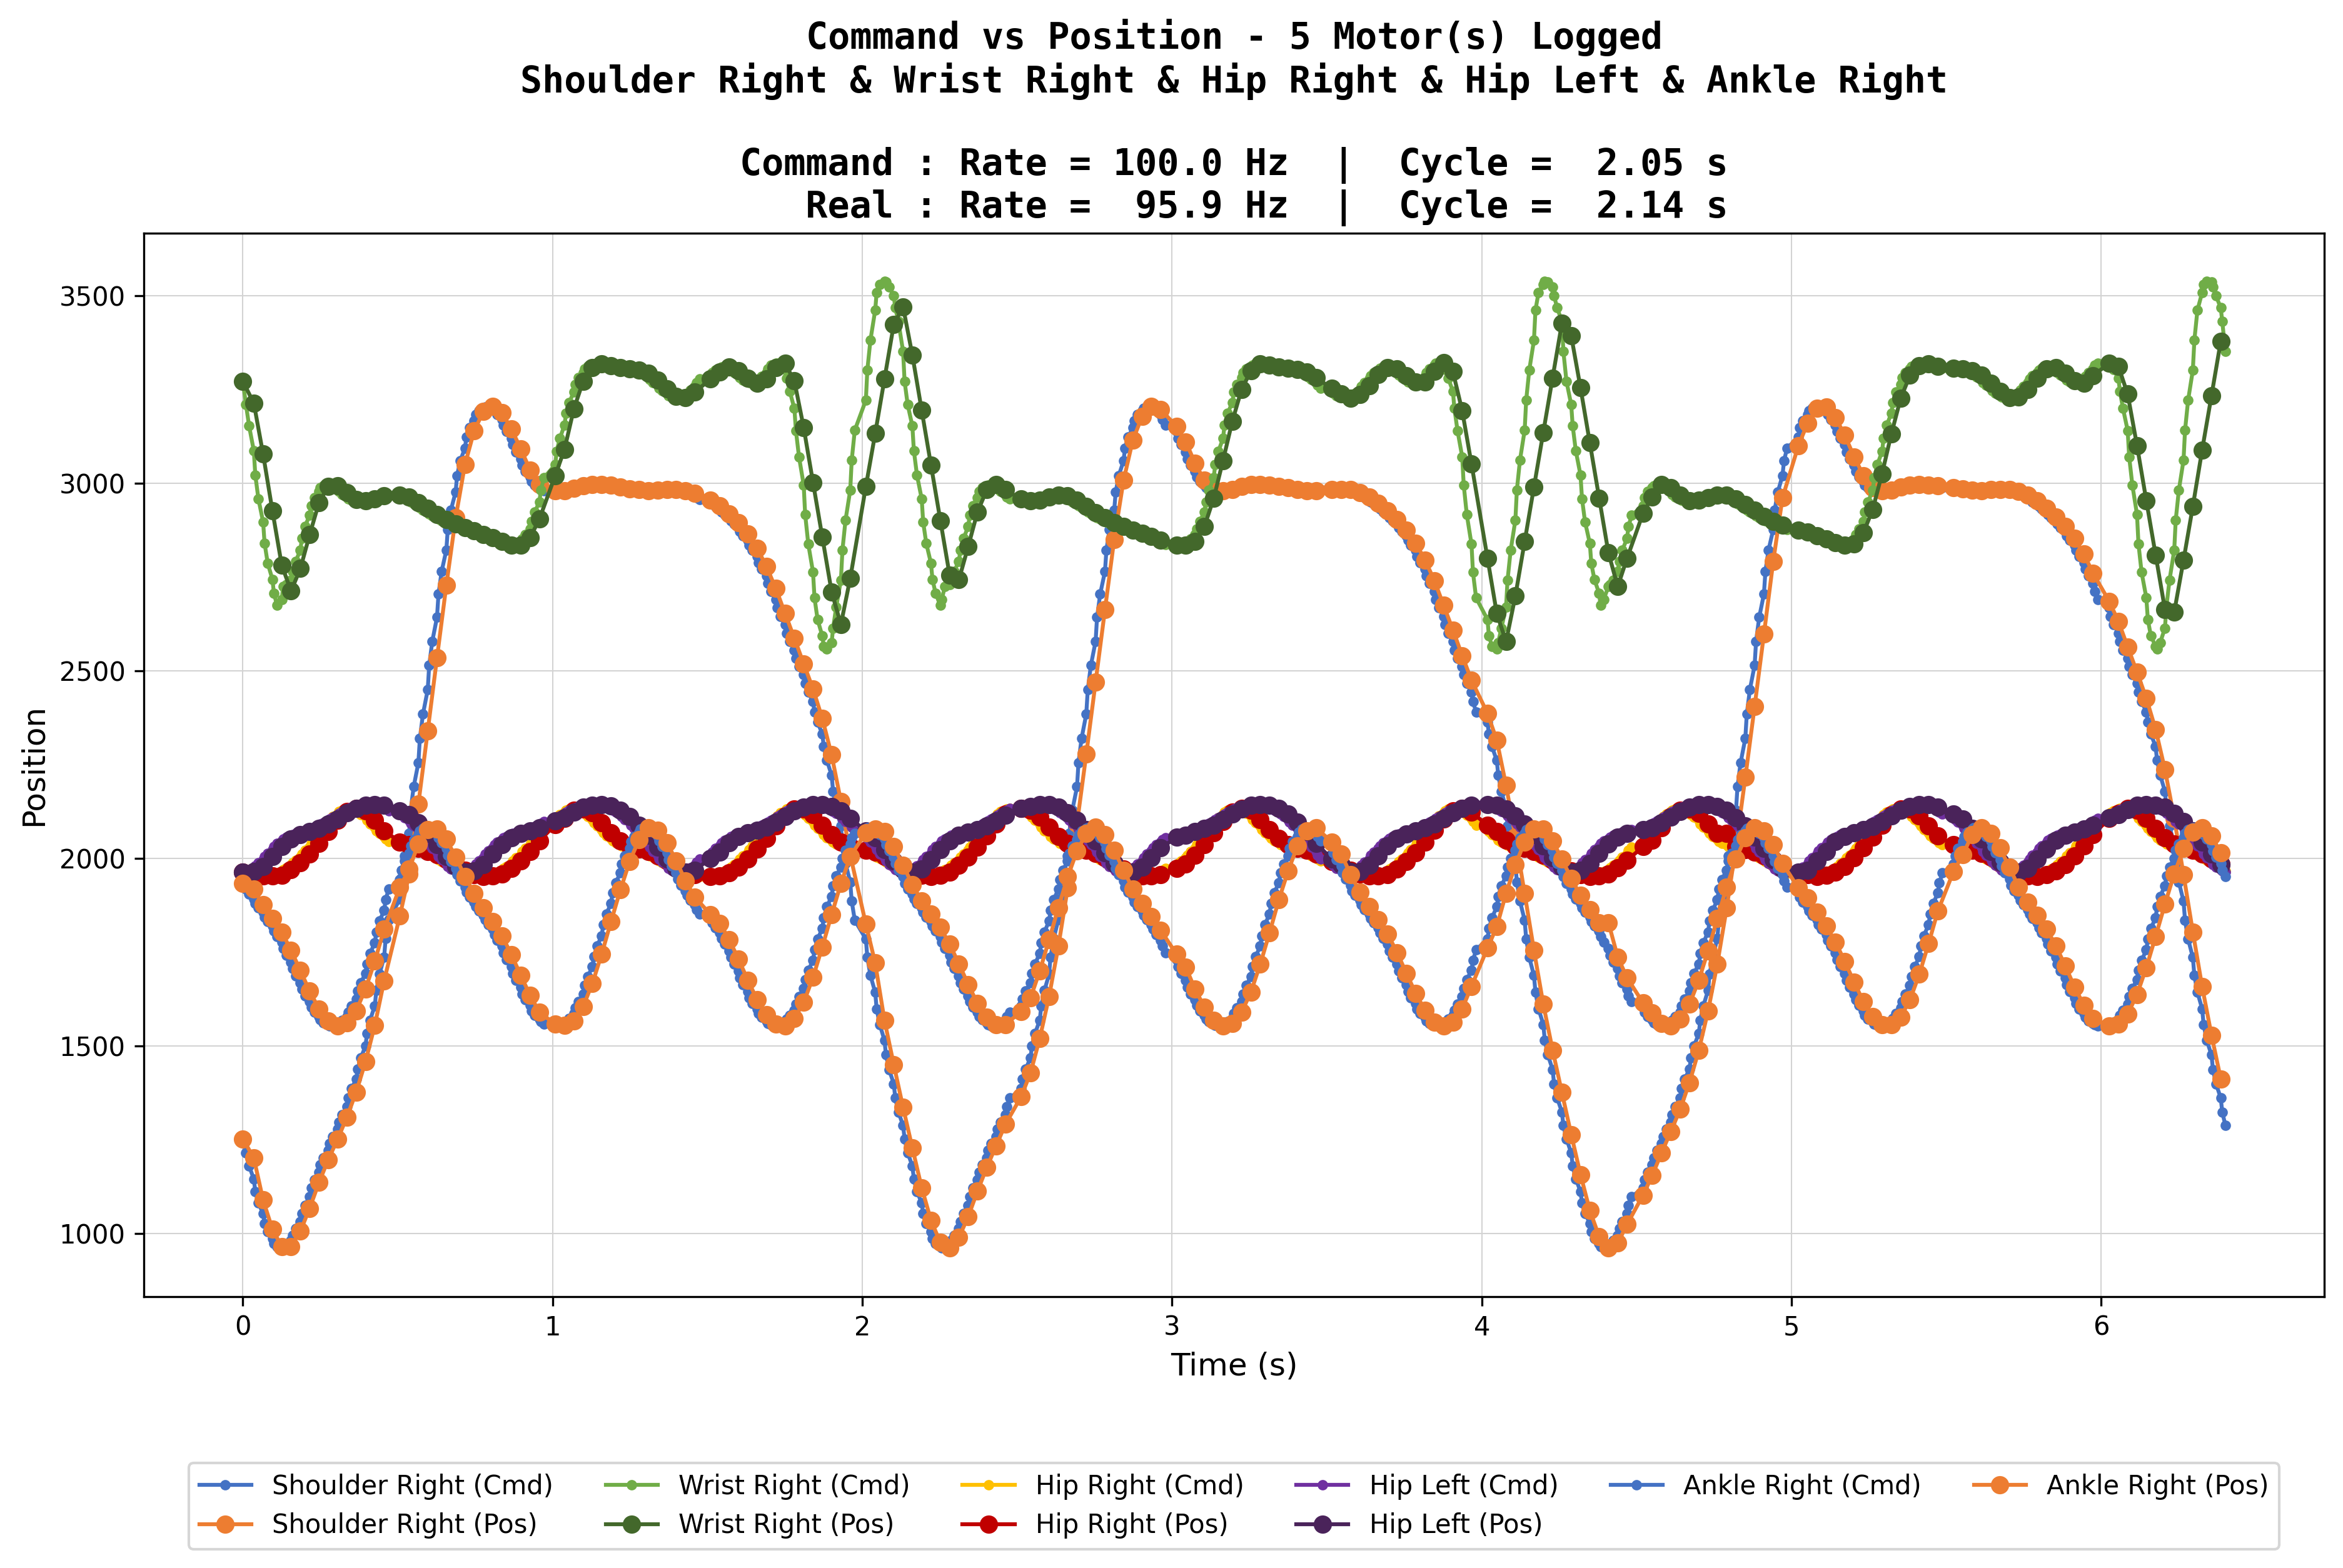
\includegraphics[width=\textwidth]{graphiques/log_100Hz_5mot.png}
        \caption{100\,Hz, $N = 5$ $\rightarrow$ 95.9 Hz.}
        \label{fig:log_100Hz_5mot}
    \end{subfigure}

    \caption{Sweep of the number of logged motors at different frequencies.}
    \label{fig:motor_logging_sweep}
\end{figure}



As we can see in figure~\ref{fig:motor_logging_sweep} and in the table~\ref{tab:matrix}, \textbf{at low frequency, the number of logged motors has no measurable effect on the control frequency}. At 36\,Hz, the five configurations all give 35.9--36.0\,Hz, at 100\,Hz, they stay grouped around 96\,Hz, whether we log one motor or five, this clearly shows that the problem occurs primarily at high frequencies.

\begin{table}[H]
\centering
\begin{tabular}{|c|c|c|c|c|}
\hline
\multirow{2}{*}{$N$ (motors)} & \multicolumn{4}{c|}{Real control frequency $f_{\text{real}}$ (Hz)} \\ \cline{2-5}
 & $f_c = 36$\,Hz & $f_c = 72$\,Hz & $f_c = 100$\,Hz & $f_c = 200$\,Hz \\ \hline
1 & 35.9 & 68.0 & 96.2 & 191.6 \\ \hline
2 & 35.9 & 68.1 & 96.2 & 190.7 \\ \hline
3 & 36.0 & 68.0 & 95.9 & 189.5 \\ \hline
4 & 36.0 & 68.0 & 95.9 & 187.7 \\ \hline
5 & 35.9 & 69.5 & 95.9 & \textbf{172.8} \\ \hline
\end{tabular}
\caption{Real control frequency as a function of the number of logged motors ($K = 3$ frames).}
\label{tab:matrix}
\end{table}

As we can see in the table, even below the degradation threshold, the real frequency stays slightly under the setpoint, 96.2\,Hz for a 100\,Hz target, 68\,Hz for 72\,Hz and on the order of a few percent, it is also \emph{independent of $N$} (the corresponding columns are flat). So the problem does not come from telemetry, then, but from the incompressible load run on \emph{every} frame, so the broadcast \texttt{SyncWrite}, the command interpolation, the IMU acquisition and servicing the 20\,Hz SSE stream. This background load, which we will write $t_{hk}$, caps the reachable rate regardless of how many motors are read, it should be distinguished from the extra cost, variable in $N$, of the \texttt{SyncRead} read.

These behaviors, a deficit independent of $N$ and a degradation in $N$ only at high frequency, are explained by the \emph{time budget per frame}. The control loop is a fixed-period scheduler targeting $T_c = 1/f_c$, each frame runs the background load $t_{hk}$ introduced above. Once every $K$ frames, the \texttt{SyncRead} pass of the $N$ motors is added, whose sequential bus occupancy splits into a fixed term and a term proportional to the number of responses:
\begin{equation}
\tau_{\text{read}}(N) = t_0 + N\, t_m ,
\label{eq:tauread}
\end{equation}
where $t_0$ is the fixed cost (instruction + bus turnaround) and $t_m$ the per-motor cost. The read frame therefore occupies, in total, $R(N) = t_{hk} + \tau_{\text{read}}(N)$. The crucial point is that this read only lengthens the loop \emph{if it overflows the budget} $T_c$. So the mean control period is:
\begin{equation}
\boxed{\;T_{\text{real}}(N) = T_c + \frac{\bigl(R(N) - T_c\bigr)_+}{K}\;}
\label{eq:budget}
\end{equation}
Writing $(x)_+ = \max(0, x)$ for the positive part. So the degradation therefore appears only beyond a \textbf{threshold frequency} $f^\star(N) = 1/R(N)$, above which the read frame no longer fits within its period:
\begin{itemize}
    \item \textbf{Below-threshold regime} ($T_c > R(N)$, i.e. $f_c < f^\star$): the overflow term is zero, $T_{\text{real}} = T_c$, and the real frequency is \emph{independent of $N$}. This is the regime observed at 36, 72 and 100\,Hz.
    \item \textbf{Above-threshold regime} ($T_c < R(N)$): the overflow is positive and grows with $N$, degrading the rate. This is the regime observed at 200\,Hz.
\end{itemize}

In the overflow regime, equation~\eqref{eq:budget} reduces to a \emph{linear law of the period} as a function of $N$. A least-squares fit on the points $N = 1$ to $4$ at 200\,Hz gives $R(N) \approx 5.53 + 0.11\,N$ [ms], so:
\begin{equation}
T_{\text{real}}(N) \approx 5.18 + 0.036\,N \quad [\text{ms}] \qquad (f_c = 200~\text{Hz}).
\label{eq:fit}
\end{equation}
The match with the measurements (Table~\ref{tab:model}) is remarkable: for $N = 1$ to $4$, the gap between predicted and measured frequency never exceeds $0.3$\,Hz, which \textbf{experimentally validates} the model. The fitted value $t_m \approx 0.11$\,ms/motor also confirms the benefit of the high throughput, in fact, the per-motor cost has been divided by a factor of $\sim 30$ compared with the 3--4\,ms of the previous auto-direction bus. Finally, the model predicts thresholds $f^\star$ between $\approx 136$\,Hz ($N = 5$) and $\approx 177$\,Hz ($N = 1$), so it becomes immediately clear why 100\,Hz ($T_c = 10$\,ms) stays completely safe from degradation for any $N$, while 200\,Hz ($T_c = 5$\,ms) falls squarely into the overflow regime.

\begin{table}[H]
\centering
\begin{tabular}{|c|c|c|c|}
\hline
$N$ & $f_{\text{real}}$ measured (Hz) & $f_{\text{real}}$ predicted (Hz) & Gap (Hz) \\ \hline
1 & 191.6 & 191.8 & $+0.2$ \\ \hline
2 & 190.7 & 190.5 & $-0.2$ \\ \hline
3 & 189.5 & 189.2 & $-0.3$ \\ \hline
4 & 187.7 & 187.9 & $+0.2$ \\ \hline
5 & \textbf{172.8} & \textit{186.7} & \textbf{$-13.9$} \\ \hline
\end{tabular}
\caption{200\,Hz regime: measured frequency and prediction of the budget model~\eqref{eq:budget}.}
\label{tab:model}
\end{table}

The point $N = 5$ at 200\,Hz, the last row of table~\ref{tab:model}, breaks the linear law because the frequency falls to 172.8\,Hz where the model expected $\approx 186.7$\,Hz. Beyond four motors, the read-frame occupancy grows faster than the $N\,t_m$ term so the read is no longer just overflowing, it saturates, with the cost of the most distal motor in the chain approaching the timeout threshold. In practice, to stay in the degradation-free regime, just pick the rate and the number of logged motors so that $R(N) \le T_c$. At 200\,Hz we therefore keep $N \le 4$ per read group (less than $7\%$ loss), while at 100\,Hz or below, logging is "free" regardless of the number of motors. This is what justifies the combination of spatial selection and round-robin reading introduced earlier so it keeps $N$ small \emph{per read cycle} while still monitoring a large number of joints.

The last check needed in the degraded regime (200\,Hz, $N = 5$) was the rate loss stationary. So I replayed this configuration while progressively lengthening the recording duration, from $\sim$7\,s to $\sim$47\,s (figure~\ref{fig:cumulatif_part1} and figure~\ref{fig:cumulatif_part2}). Finally across all these runs, the control frequency stays confined to $173.8 \pm 0.6$\,Hz, a spread under $1\%$ and \emph{independent} of the duration. We can conclude that the degradation is therefore not cumulative, it is a fixed extra cost per read cycle, re-evaluated identically at each pass, with no memory or accumulated delay, and the command/position tracking repeats identically from one swimming cycle to the next. This confirms the time-invariance of model~\eqref{eq:budget}, where $f_{\text{real}}$ depends only on $N$, $K$ and $f_c$, not on the elapsed time.

\begin{figure}[H]
    \centering
    \begin{subfigure}[b]{0.49\textwidth}
        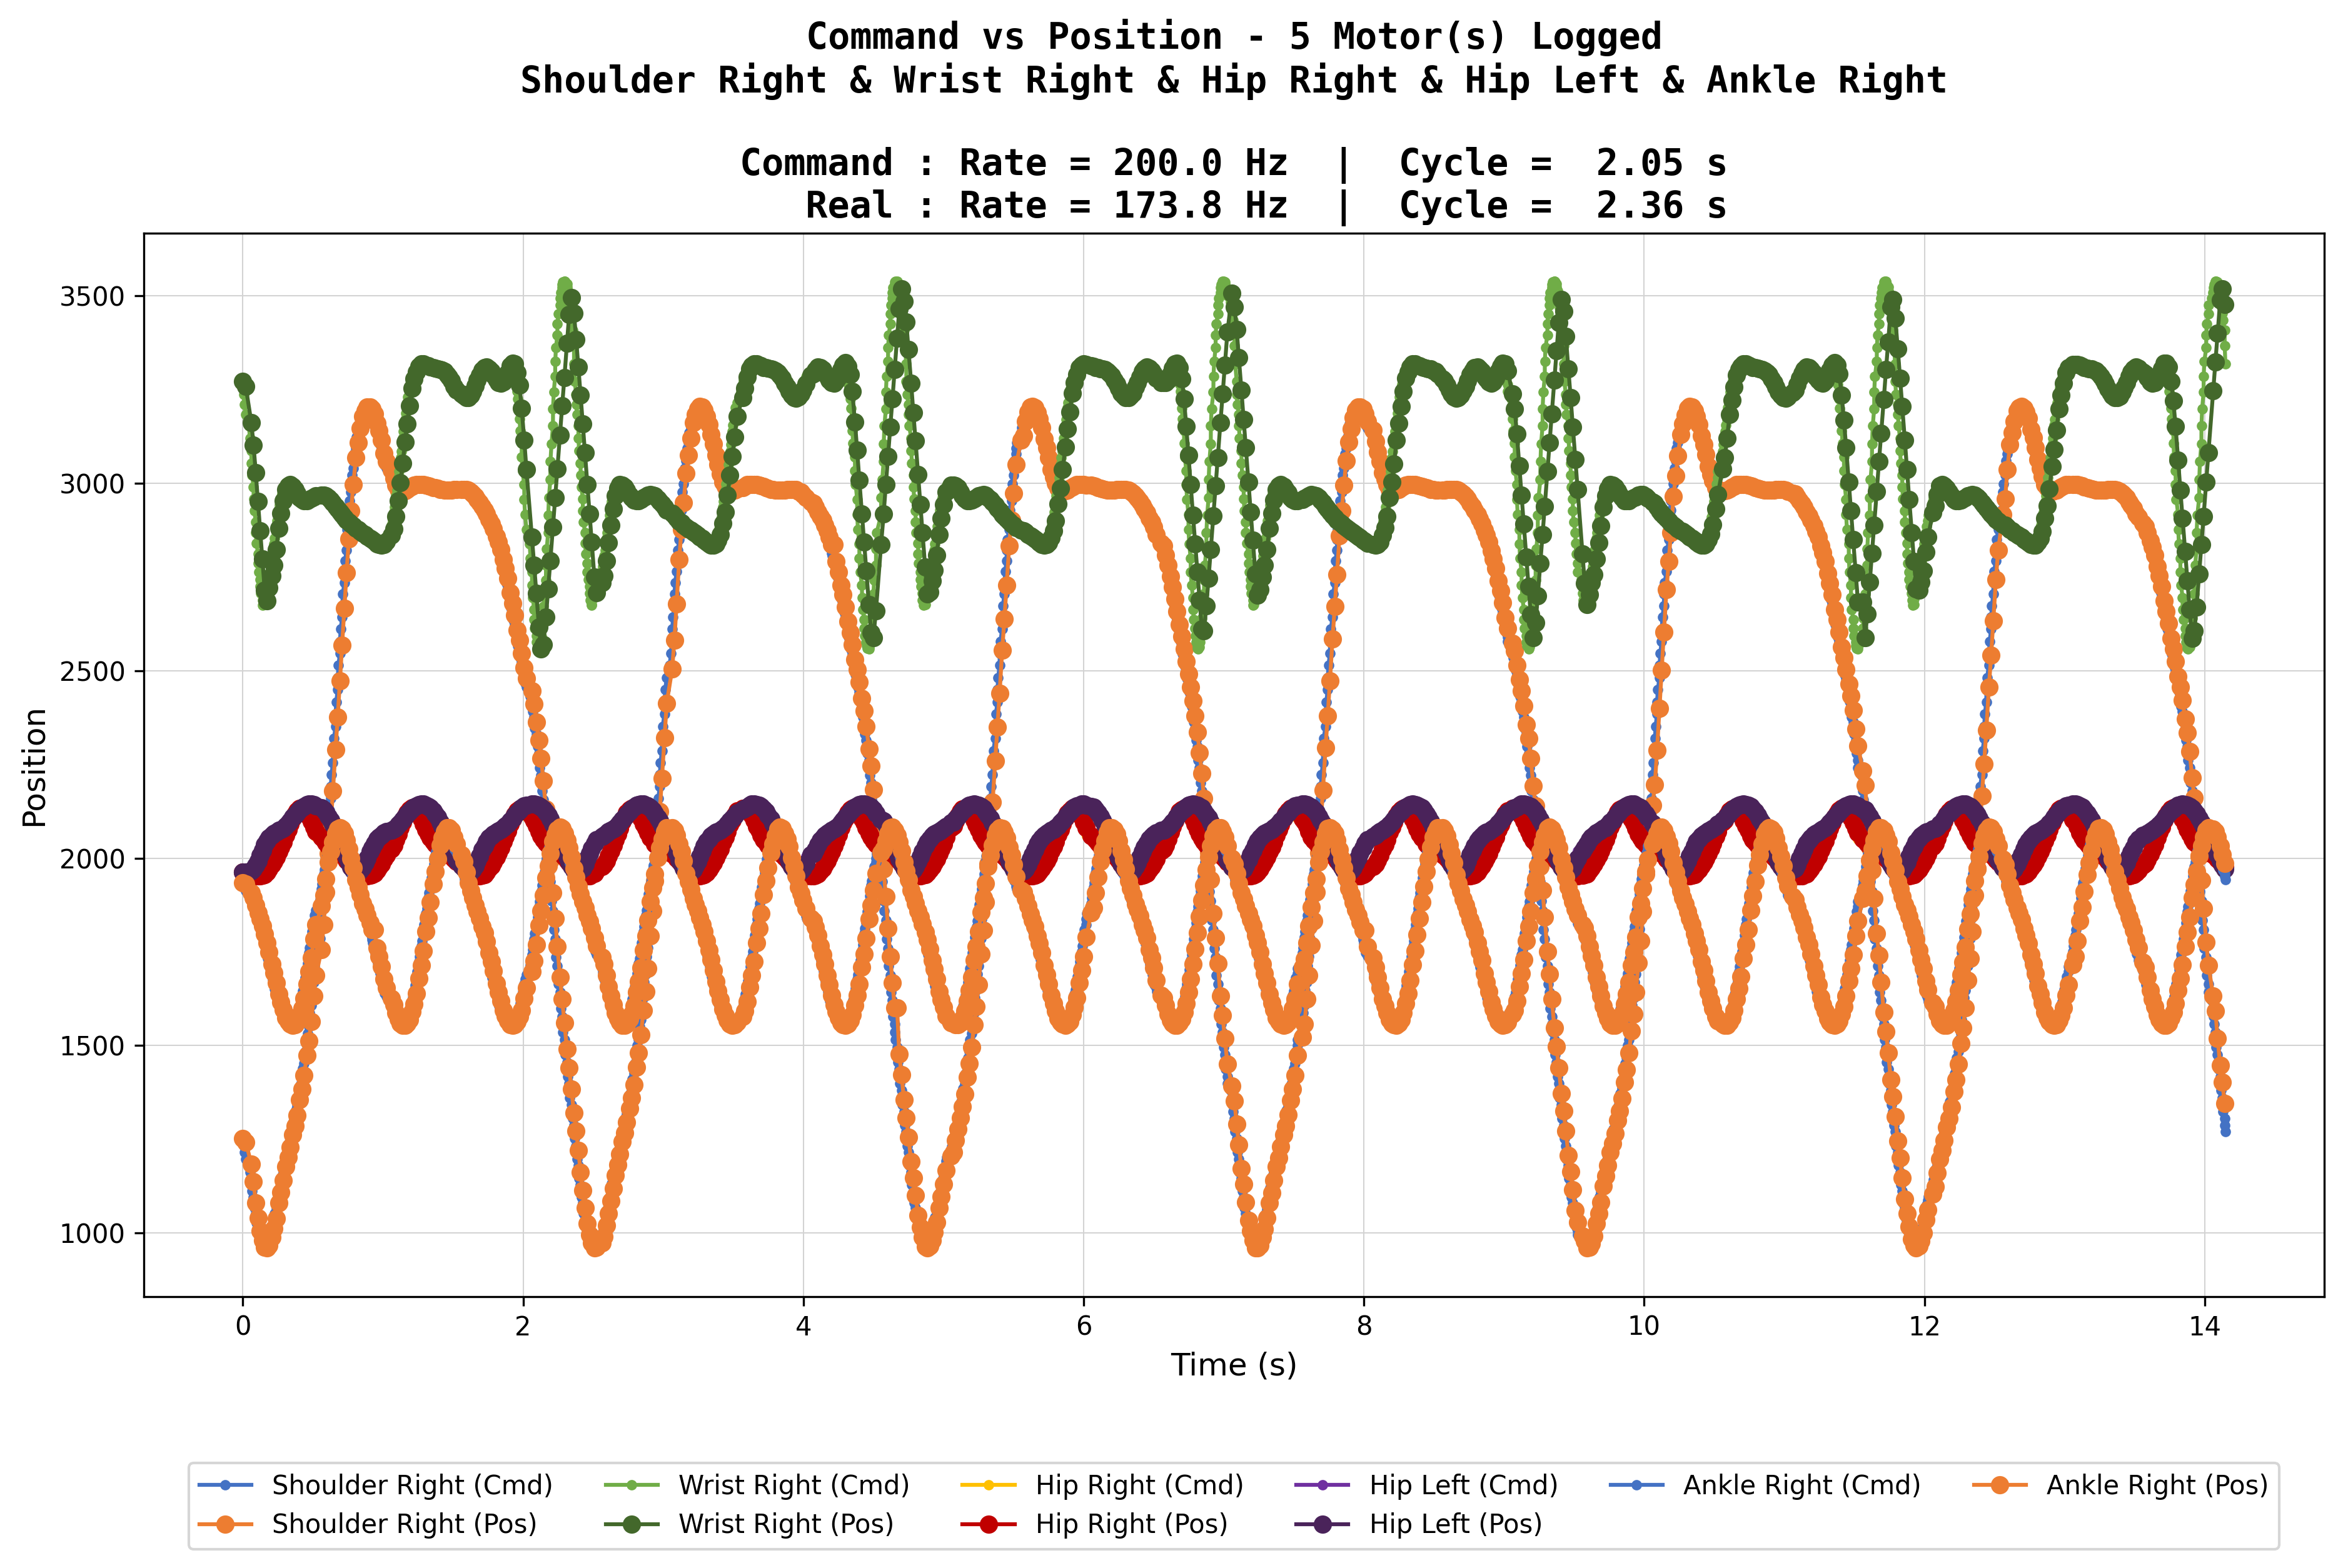
\includegraphics[width=\textwidth]{graphiques/log_5mot_dur1.png}
        \caption{$\sim$14\,s $\rightarrow$ 173.8 Hz.}
    \end{subfigure}
    \hfill
    \begin{subfigure}[b]{0.49\textwidth}
        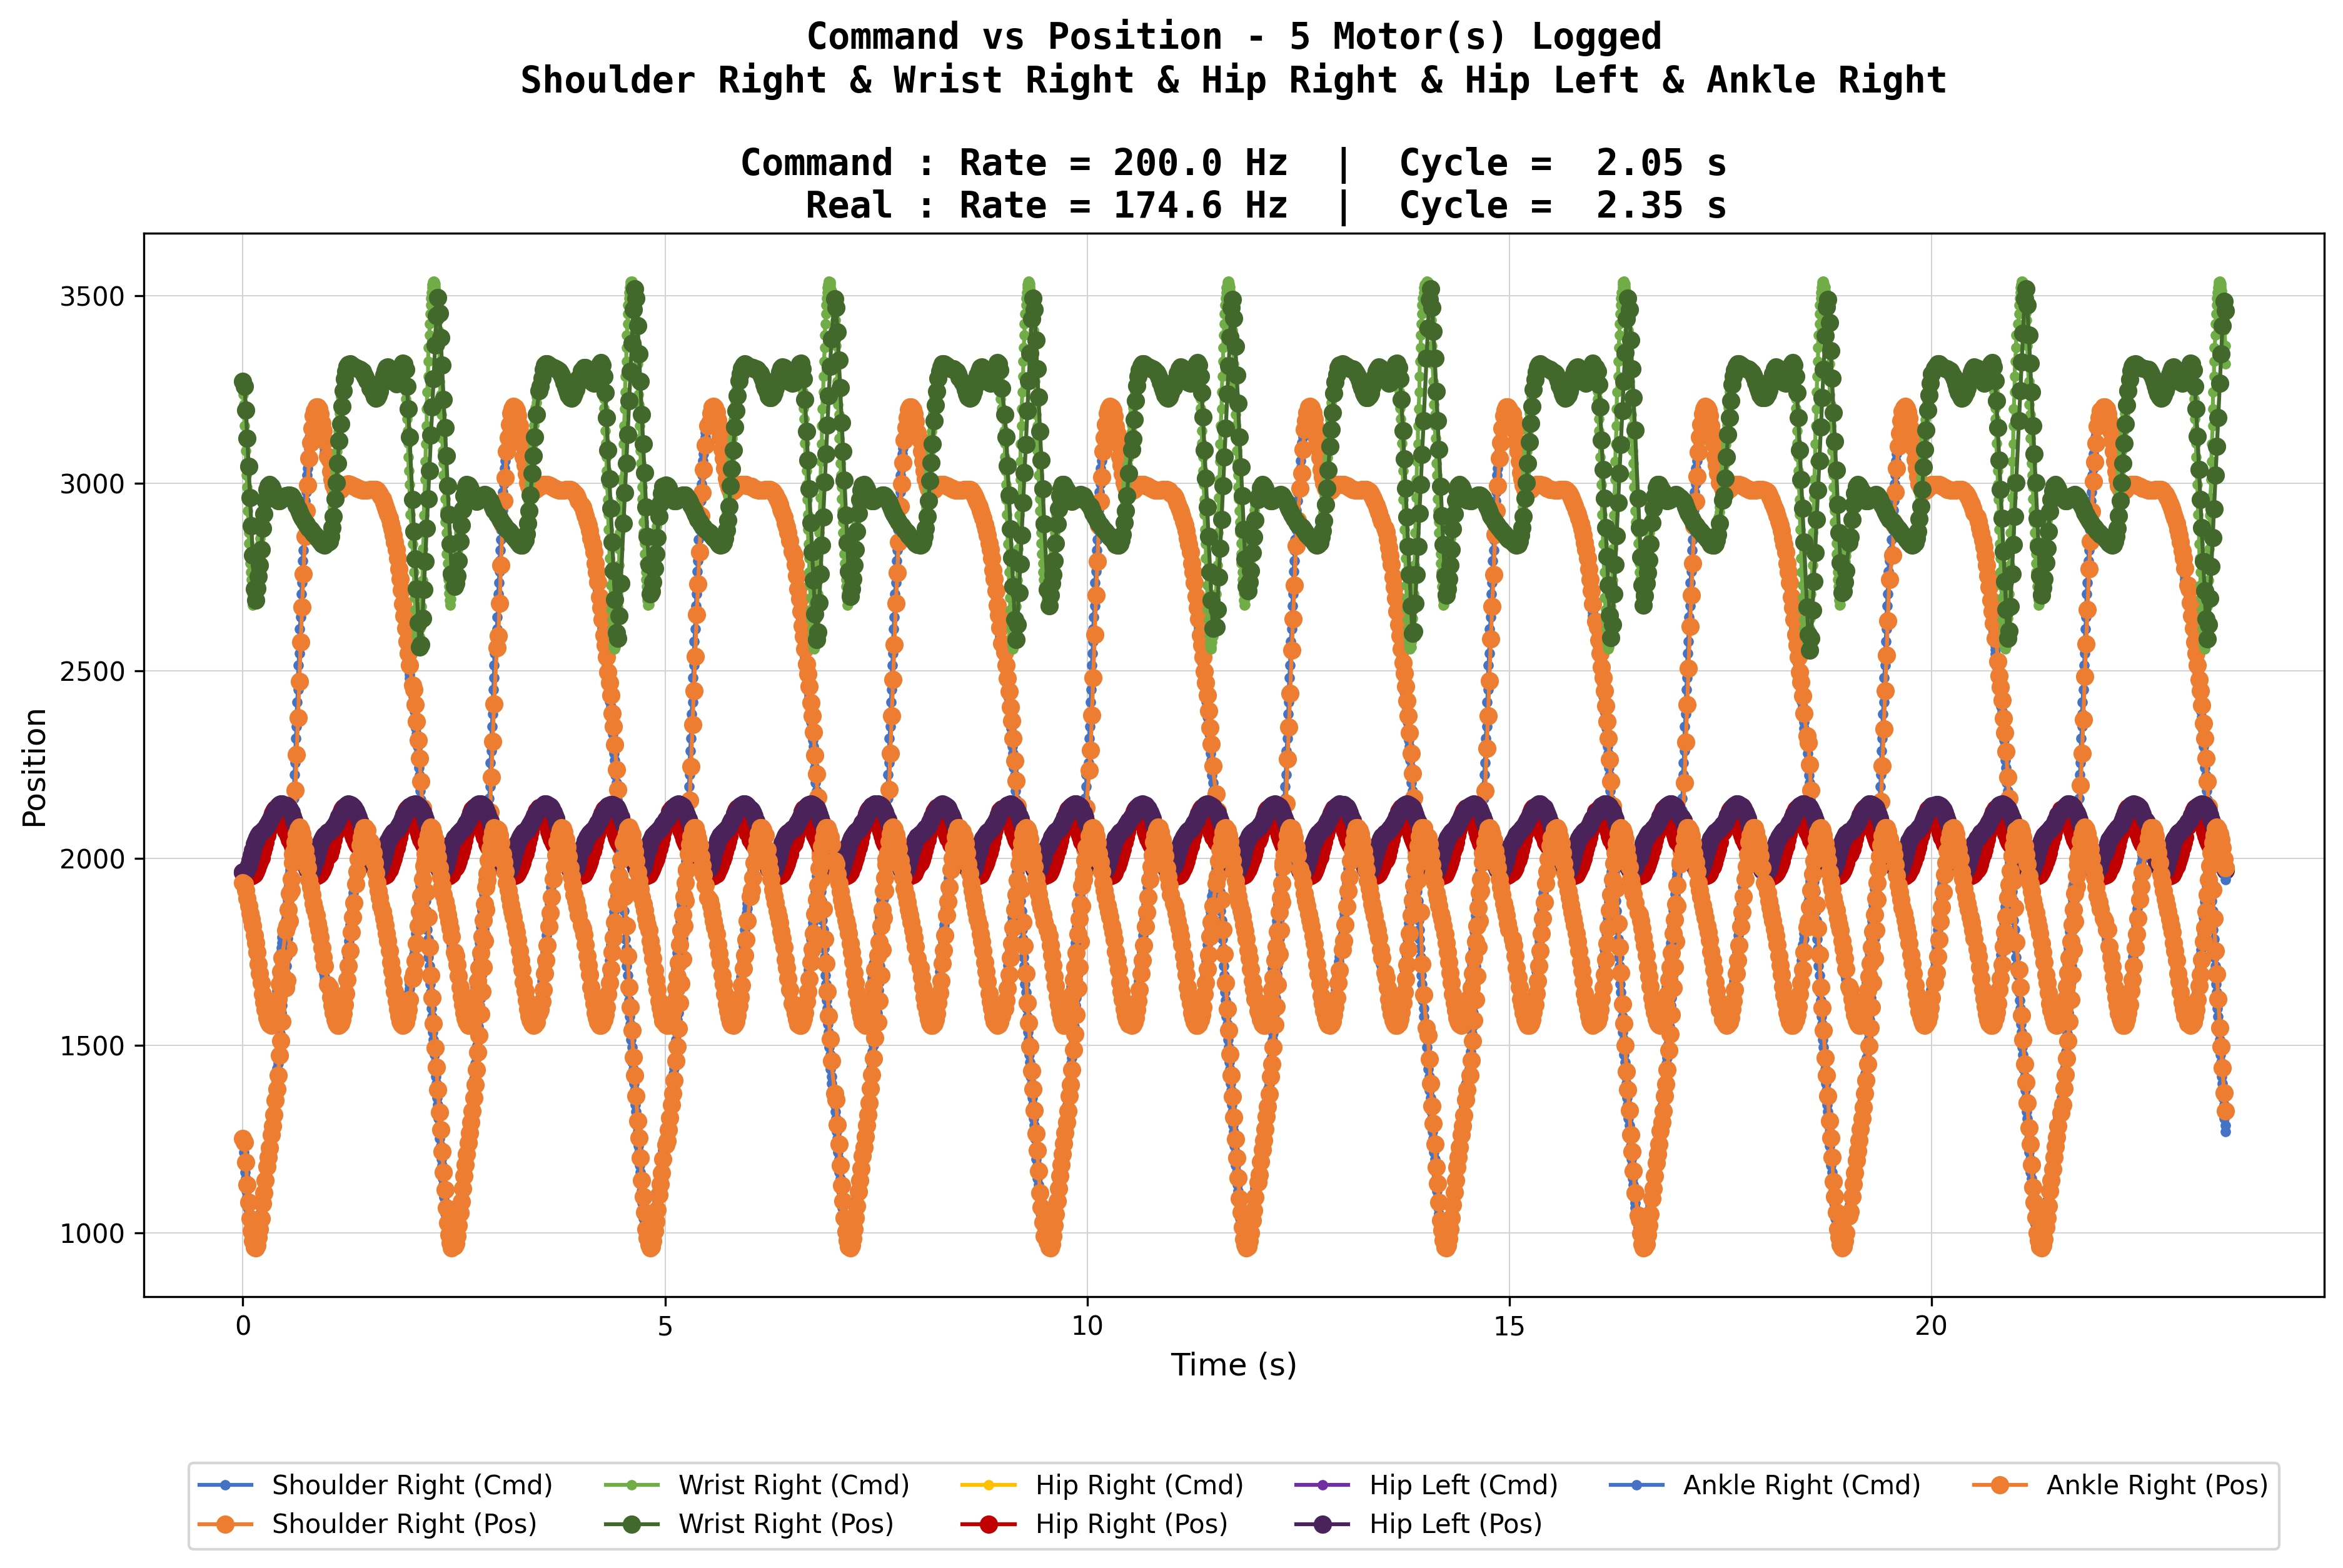
\includegraphics[width=\textwidth]{graphiques/log_5mot_dur2.png}
        \caption{$\sim$23\,s $\rightarrow$ 174.6 Hz.}
    \end{subfigure}
    \caption{Tests at different numbers of cycles at 200\,Hz, $N = 5$ (14\,s and 23\,s durations).}
    \label{fig:cumulatif_part1}
\end{figure}

\begin{figure}[H]
    \centering
    \begin{subfigure}[b]{0.49\textwidth}
        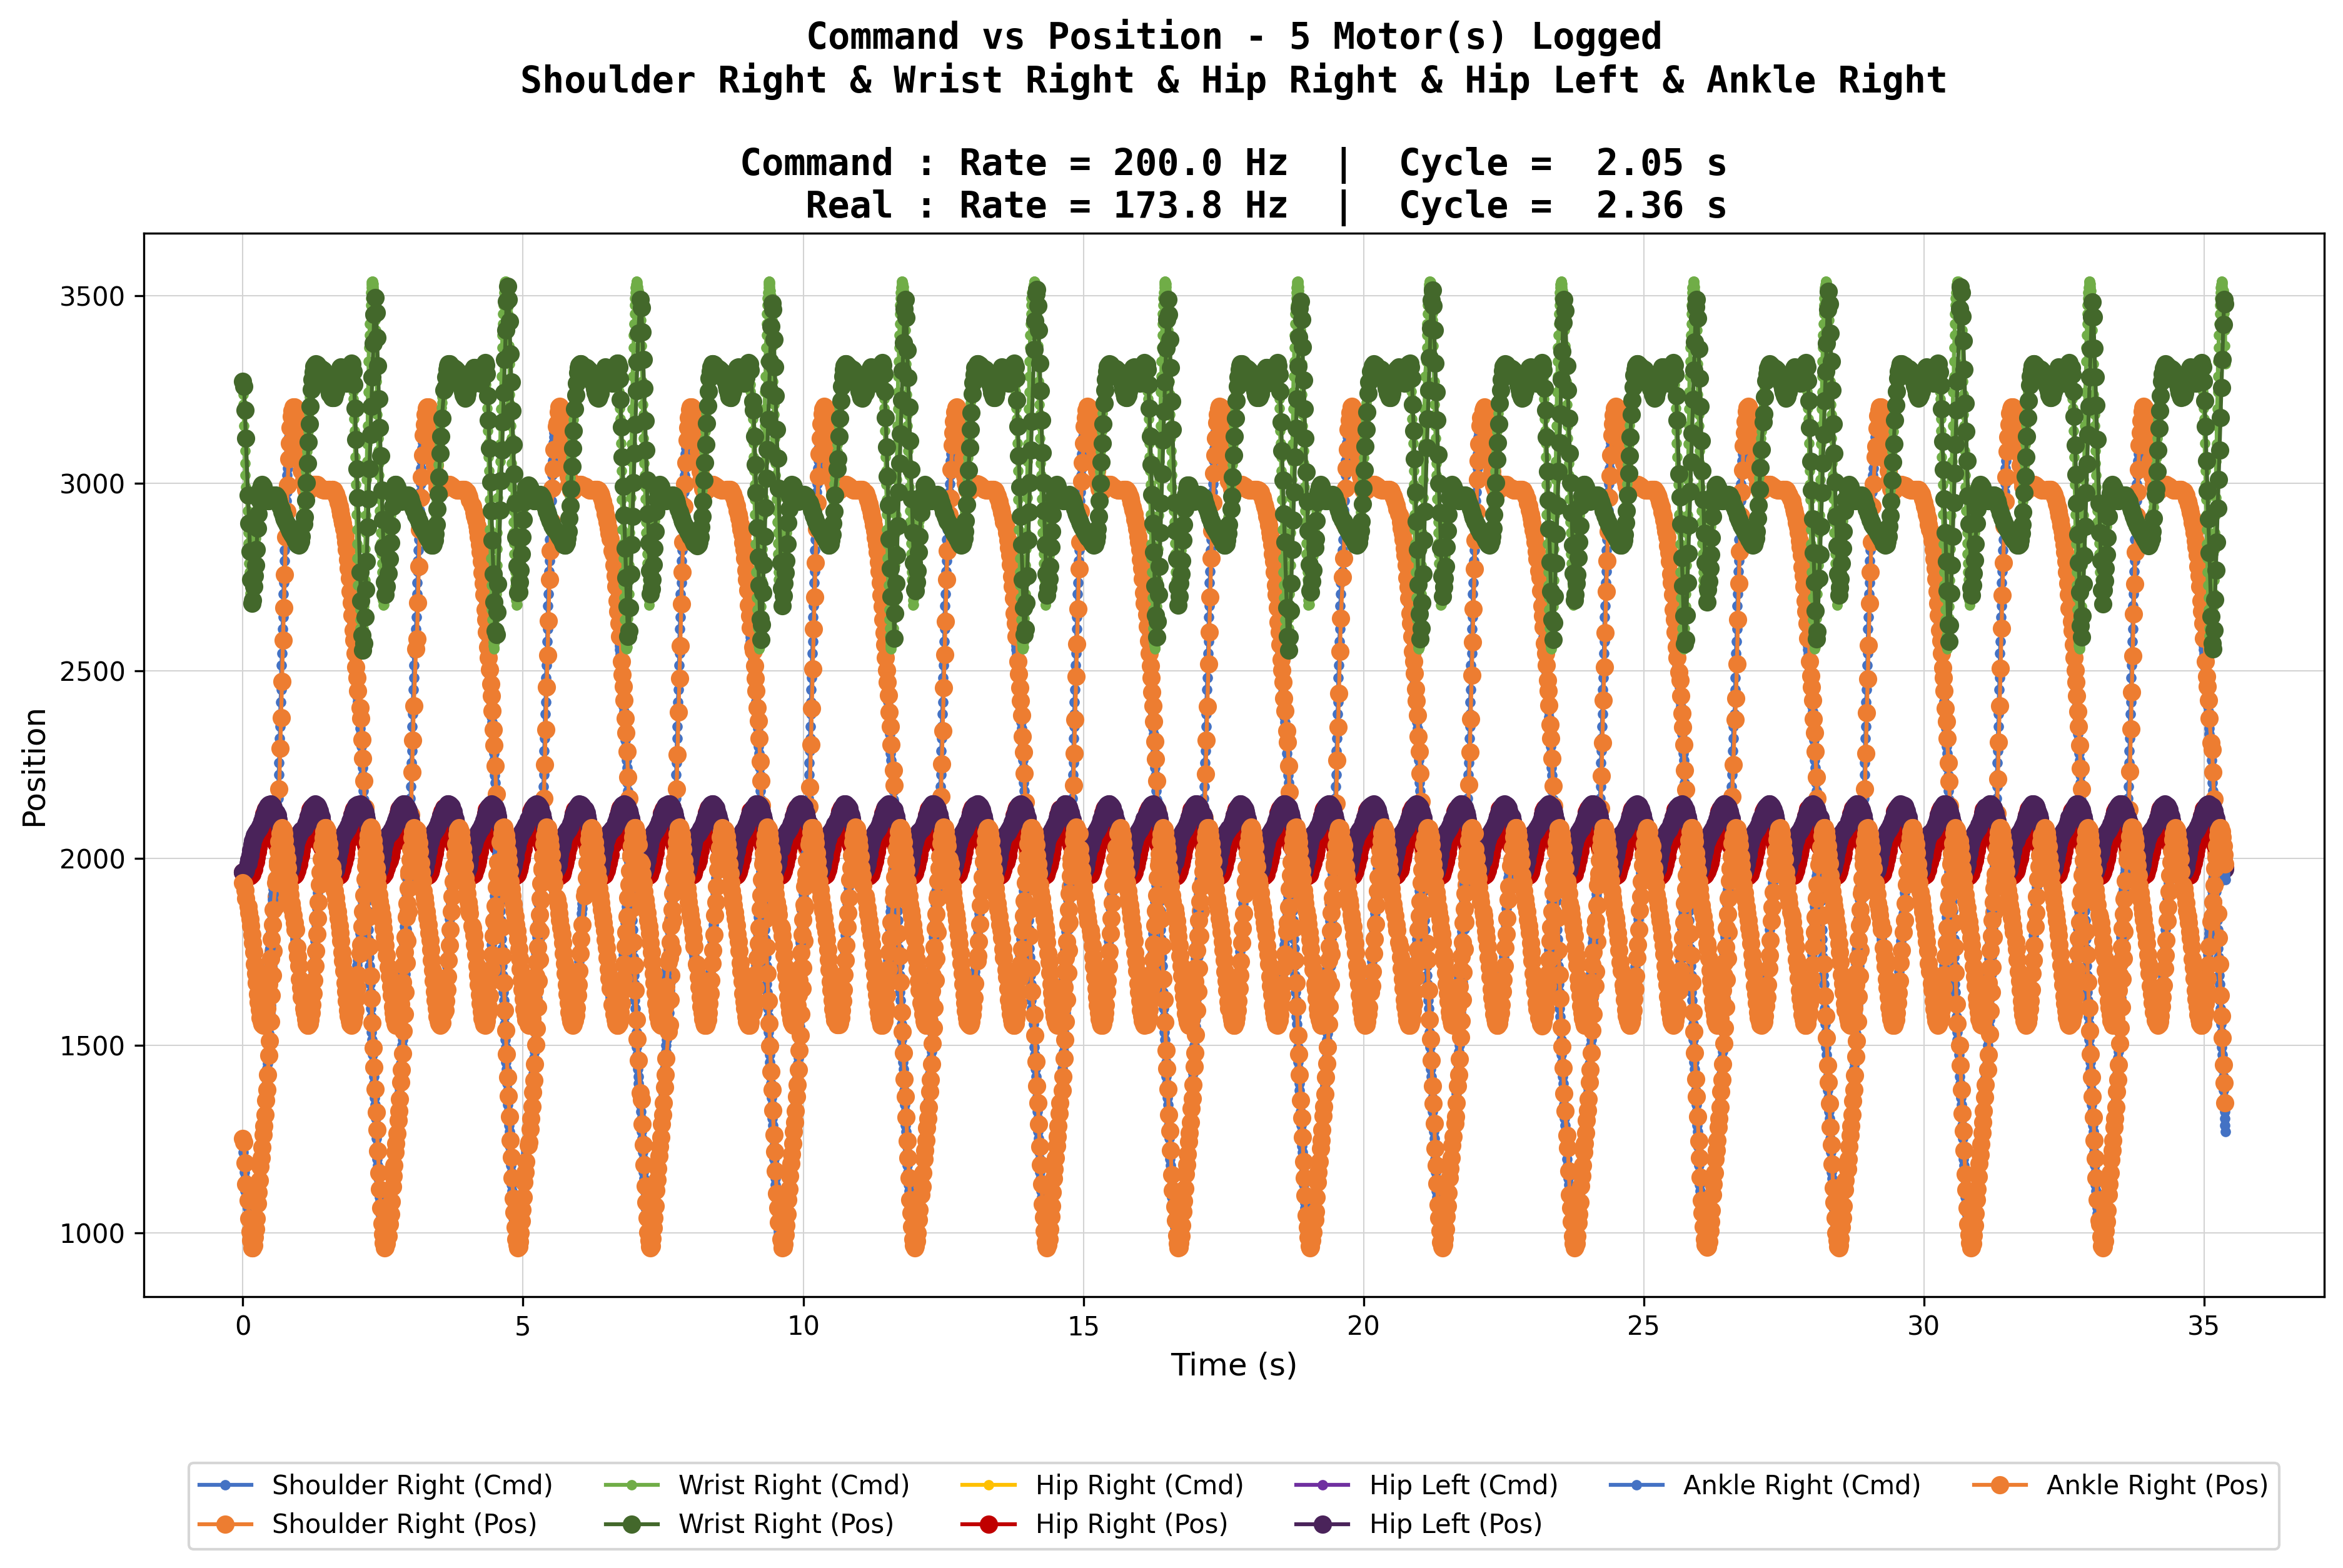
\includegraphics[width=\textwidth]{graphiques/log_5mot_dur3.png}
        \caption{$\sim$35\,s $\rightarrow$ 173.8 Hz.}
    \end{subfigure}
    \hfill
    \begin{subfigure}[b]{0.49\textwidth}
        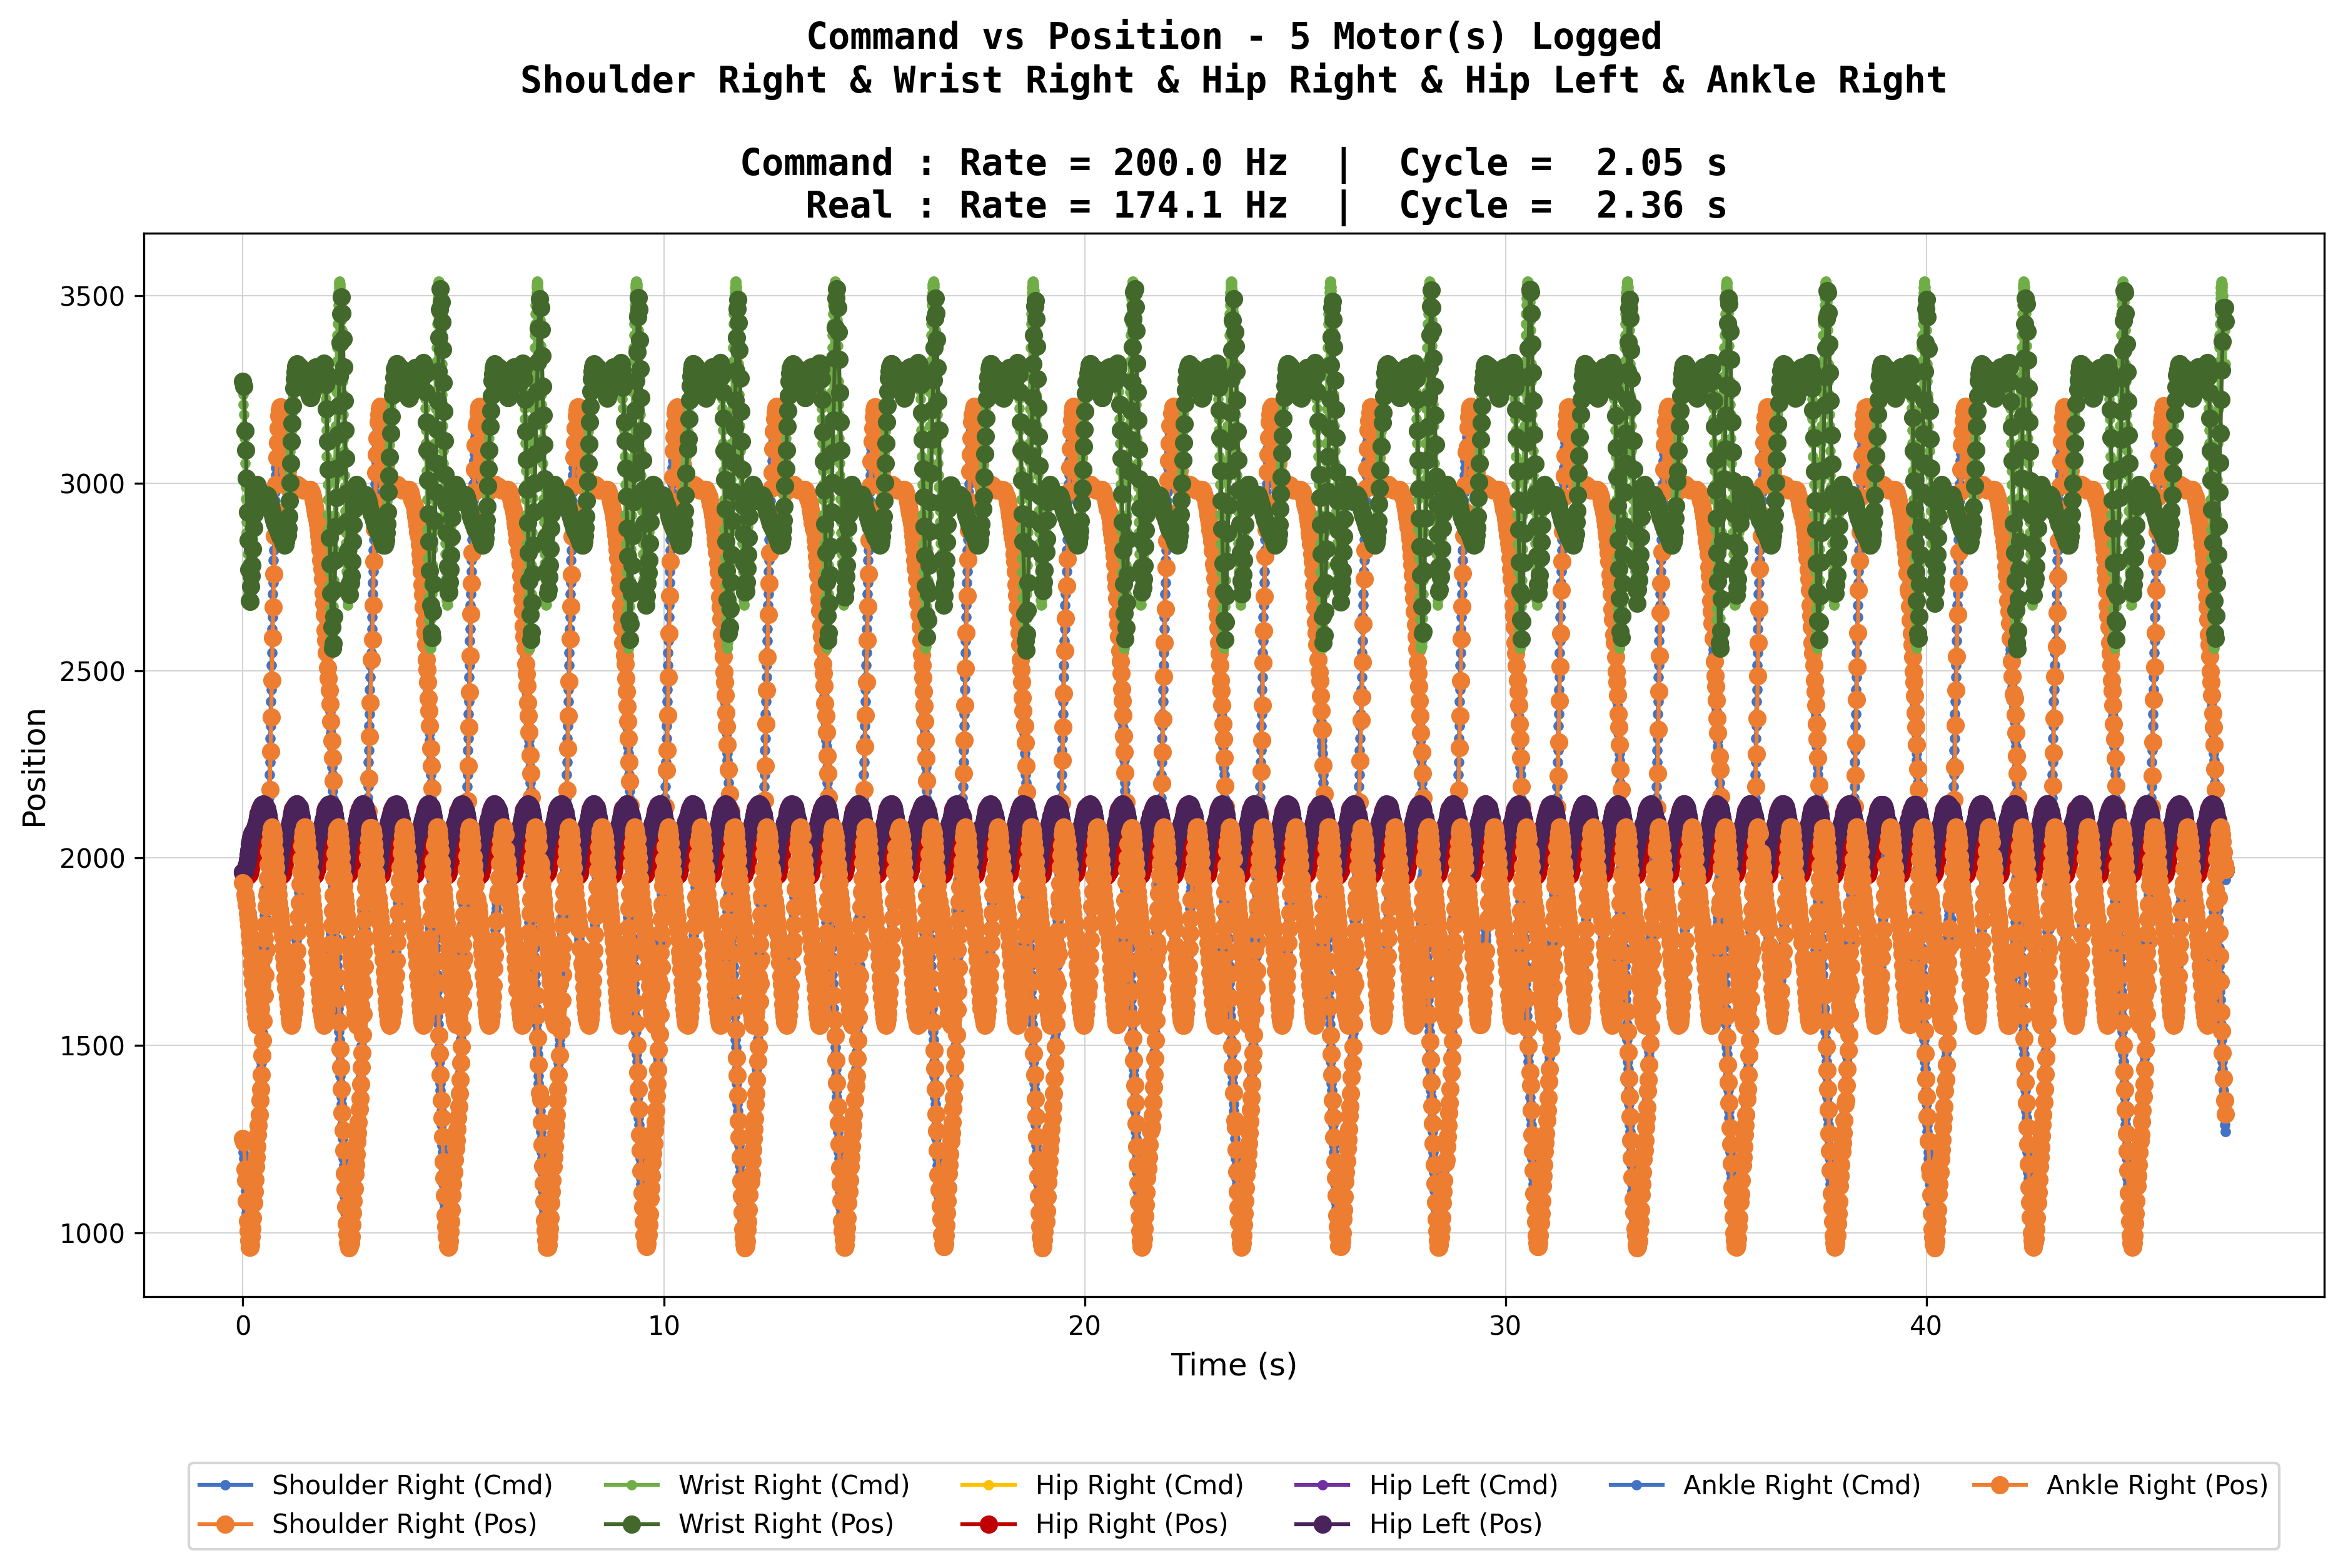
\includegraphics[width=\textwidth]{graphiques/log_5mot_dur4.png}
        \caption{$\sim$47\,s $\rightarrow$ 174.1 Hz.}
    \end{subfigure}
    \caption{Tests at different numbers of cycles at 200\,Hz, $N = 5$ (35\,s and 47\,s durations).}
    \label{fig:cumulatif_part2}
\end{figure}

\iffalse
\begin{figure}[H]
    \centering
    \begin{subfigure}[b]{0.49\textwidth}
        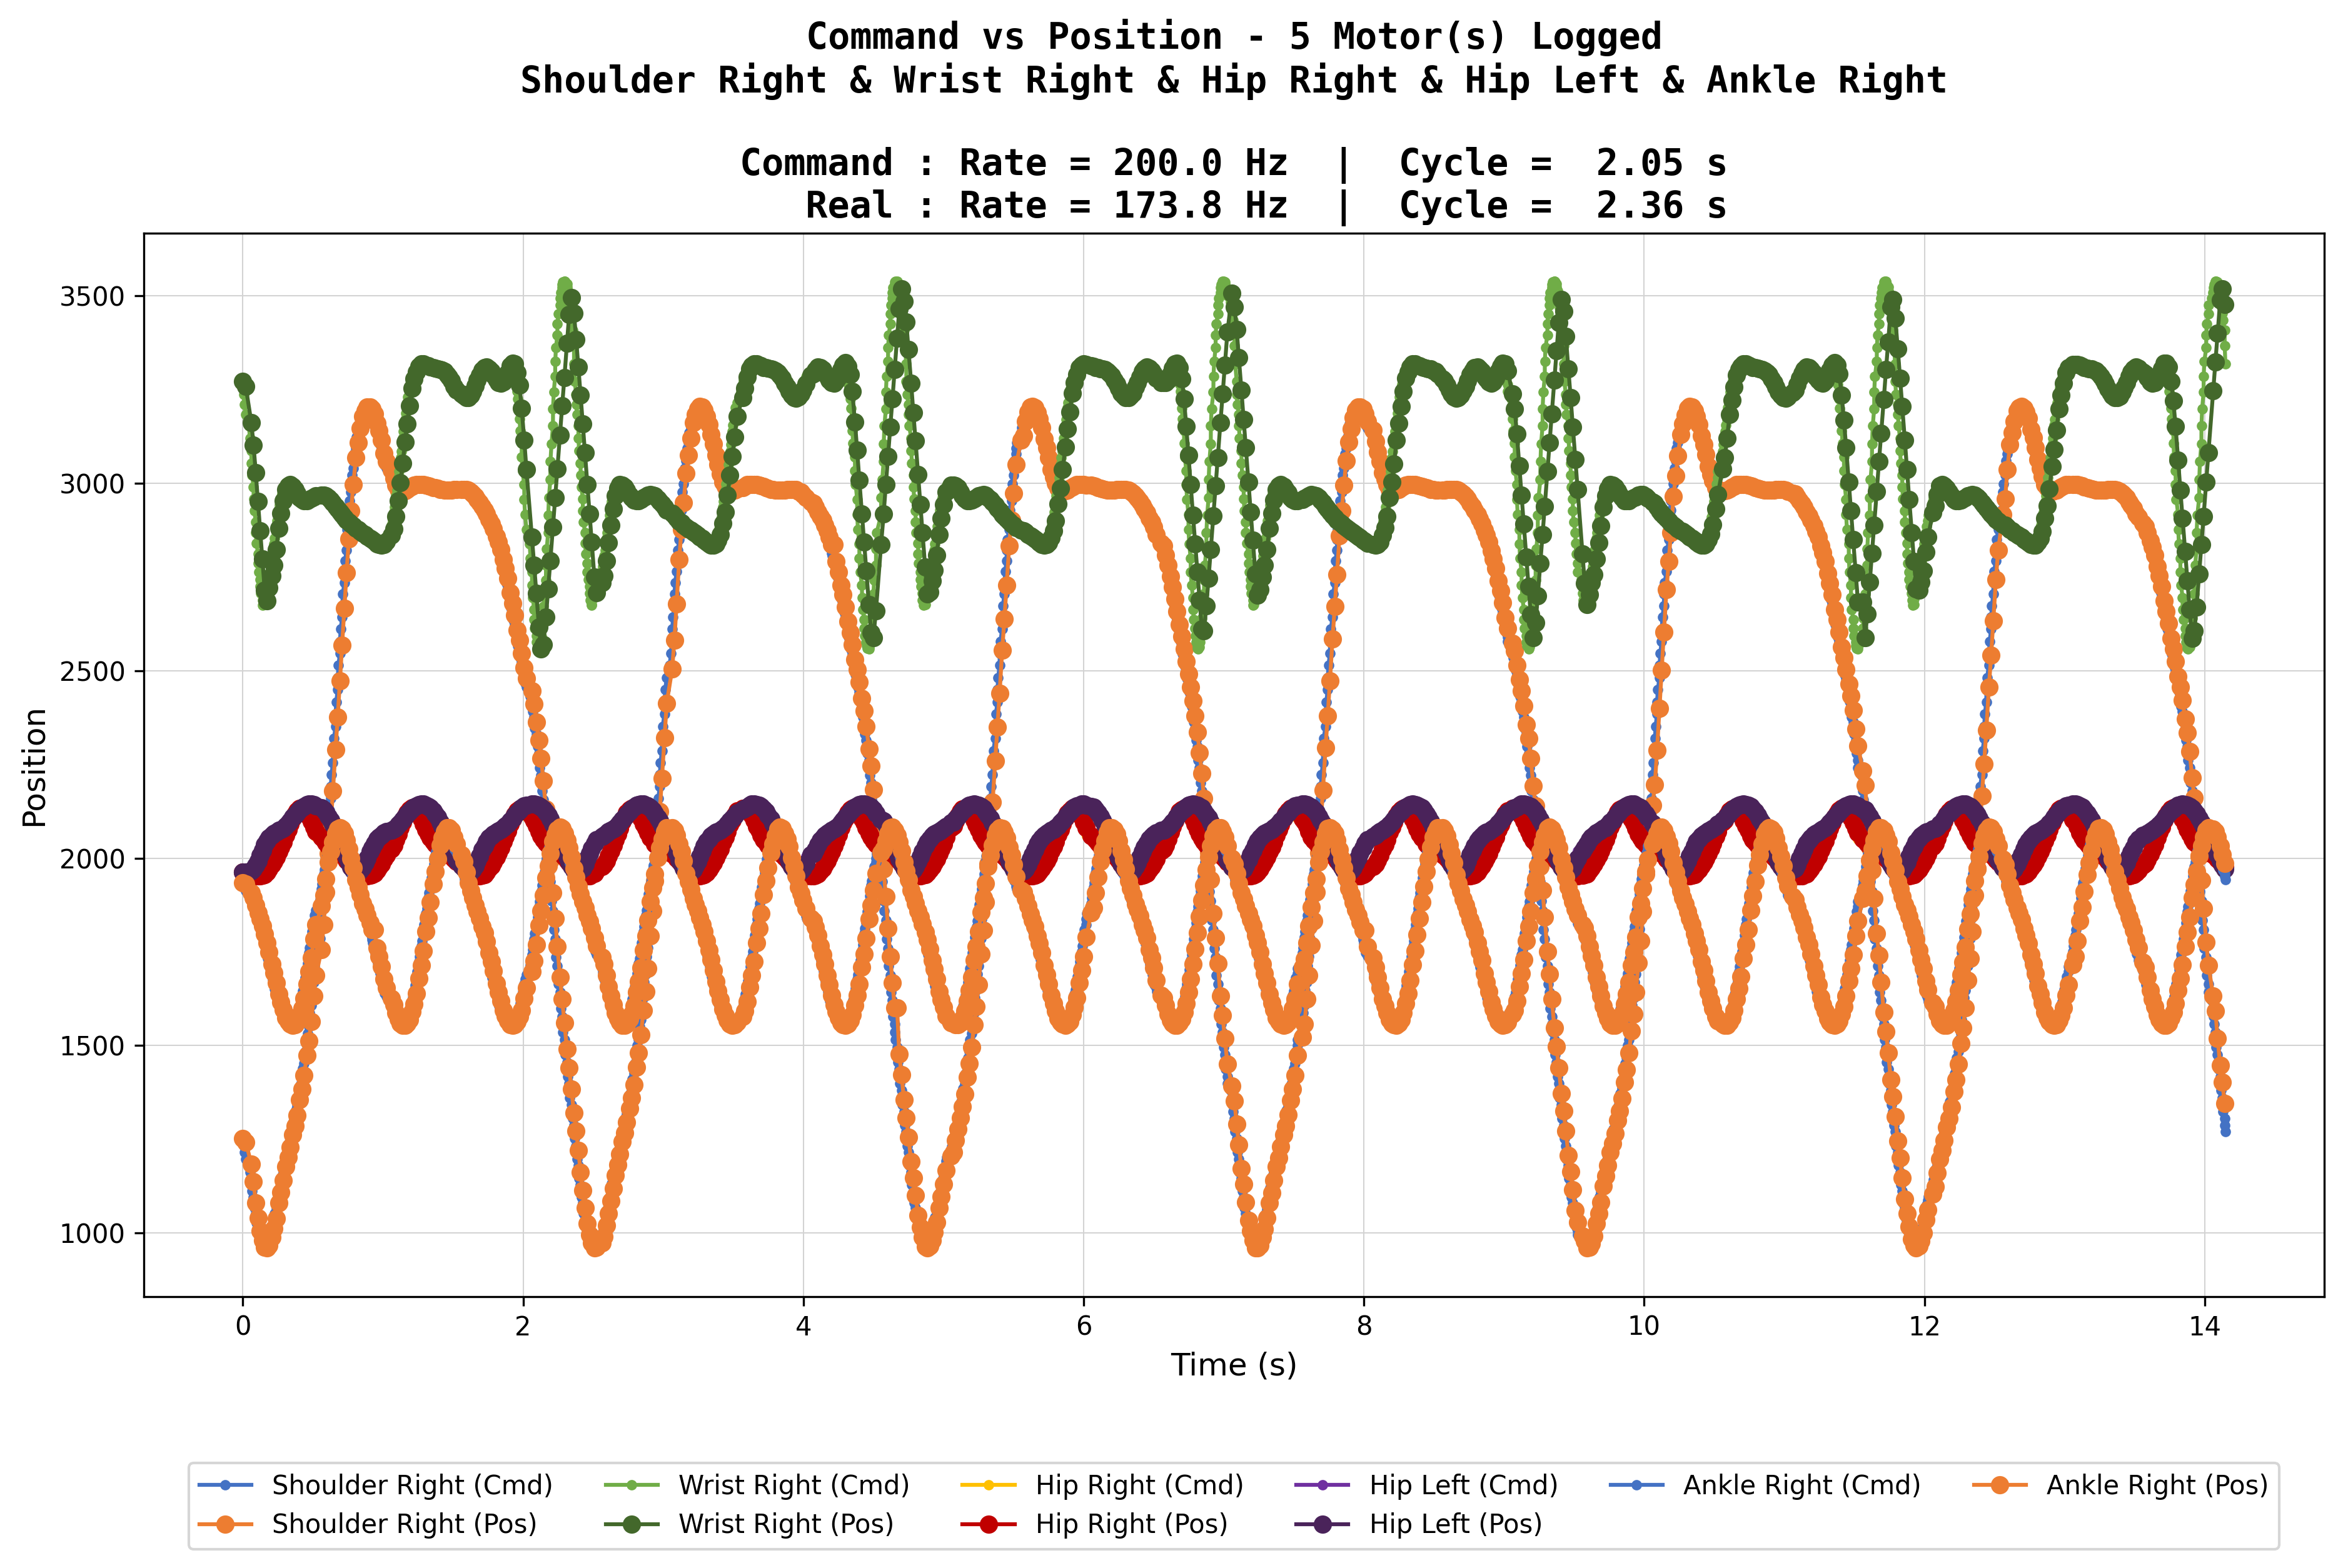
\includegraphics[width=\textwidth]{graphiques/log_5mot_dur1.png}
        \caption{$\sim$14\,s $\rightarrow$ 173.8 Hz.}
    \end{subfigure}
    \hfill
    \begin{subfigure}[b]{0.49\textwidth}
        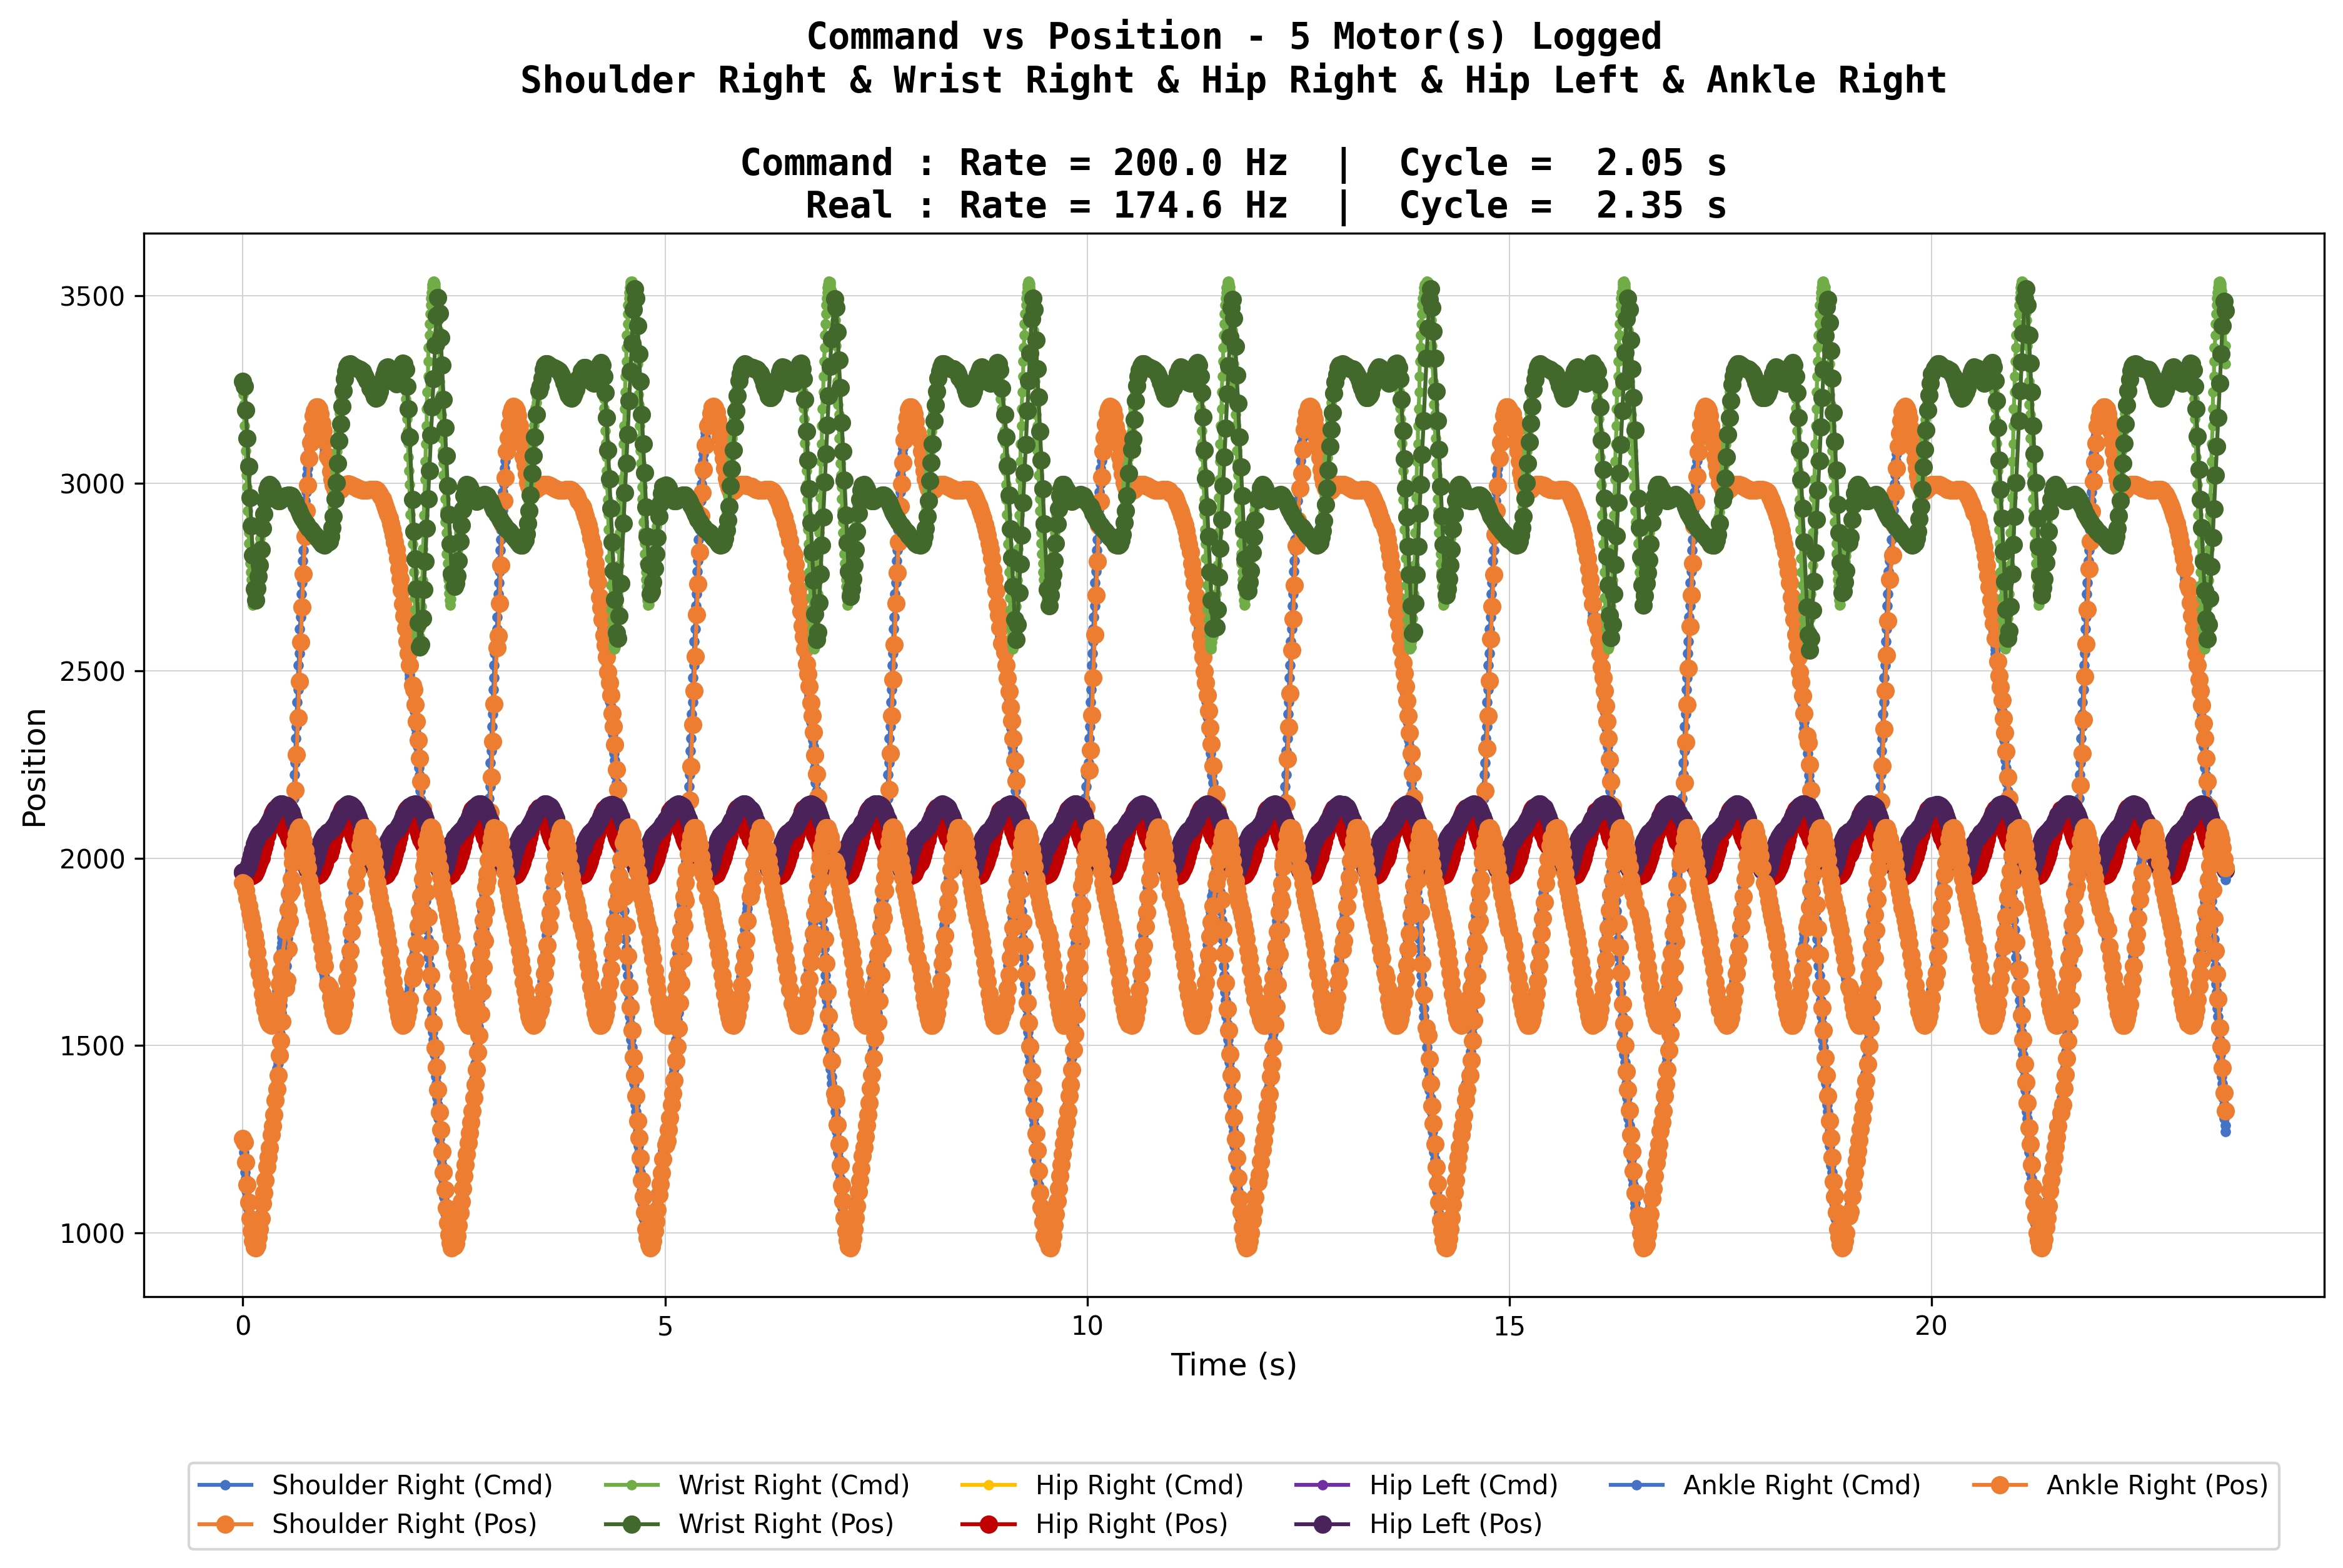
\includegraphics[width=\textwidth]{graphiques/log_5mot_dur2.png}
        \caption{$\sim$23\,s $\rightarrow$ 174.6 Hz.}
    \end{subfigure}

    \vspace{0.35em}
    \begin{subfigure}[b]{0.49\textwidth}
        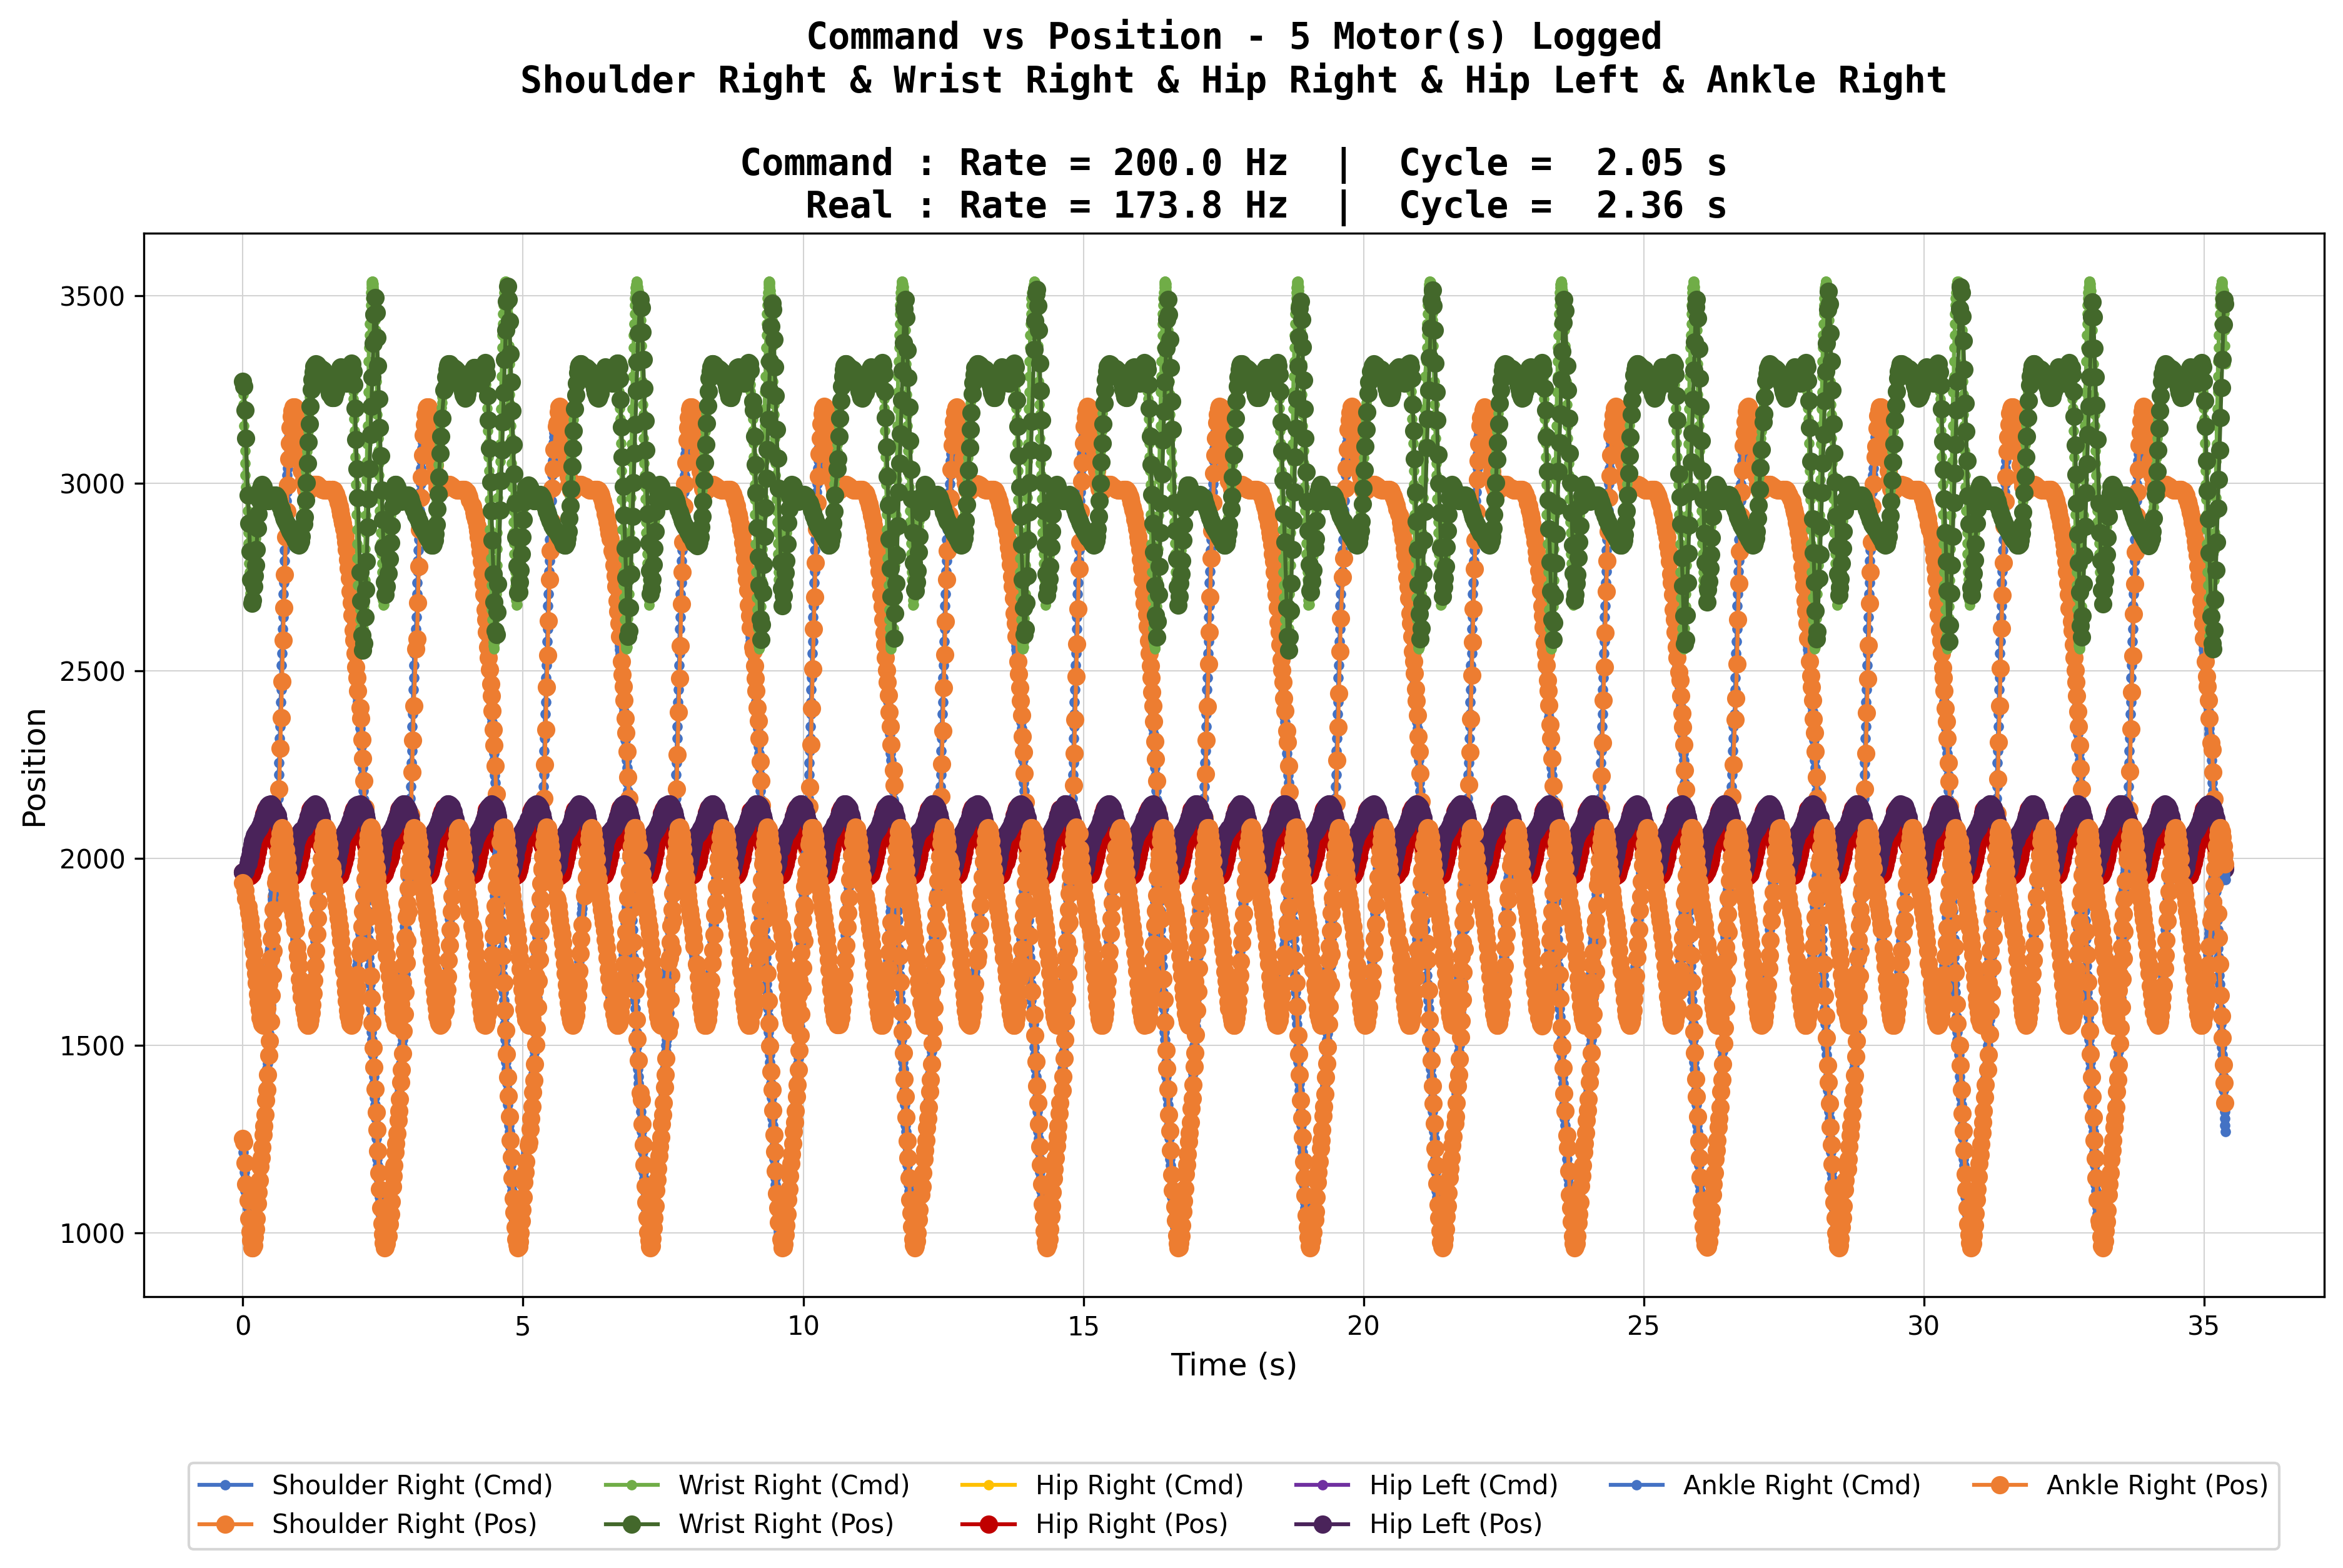
\includegraphics[width=\textwidth]{graphiques/log_5mot_dur3.png}
        \caption{$\sim$35\,s $\rightarrow$ 173.8 Hz.}
    \end{subfigure}
    \hfill
    \begin{subfigure}[b]{0.49\textwidth}
        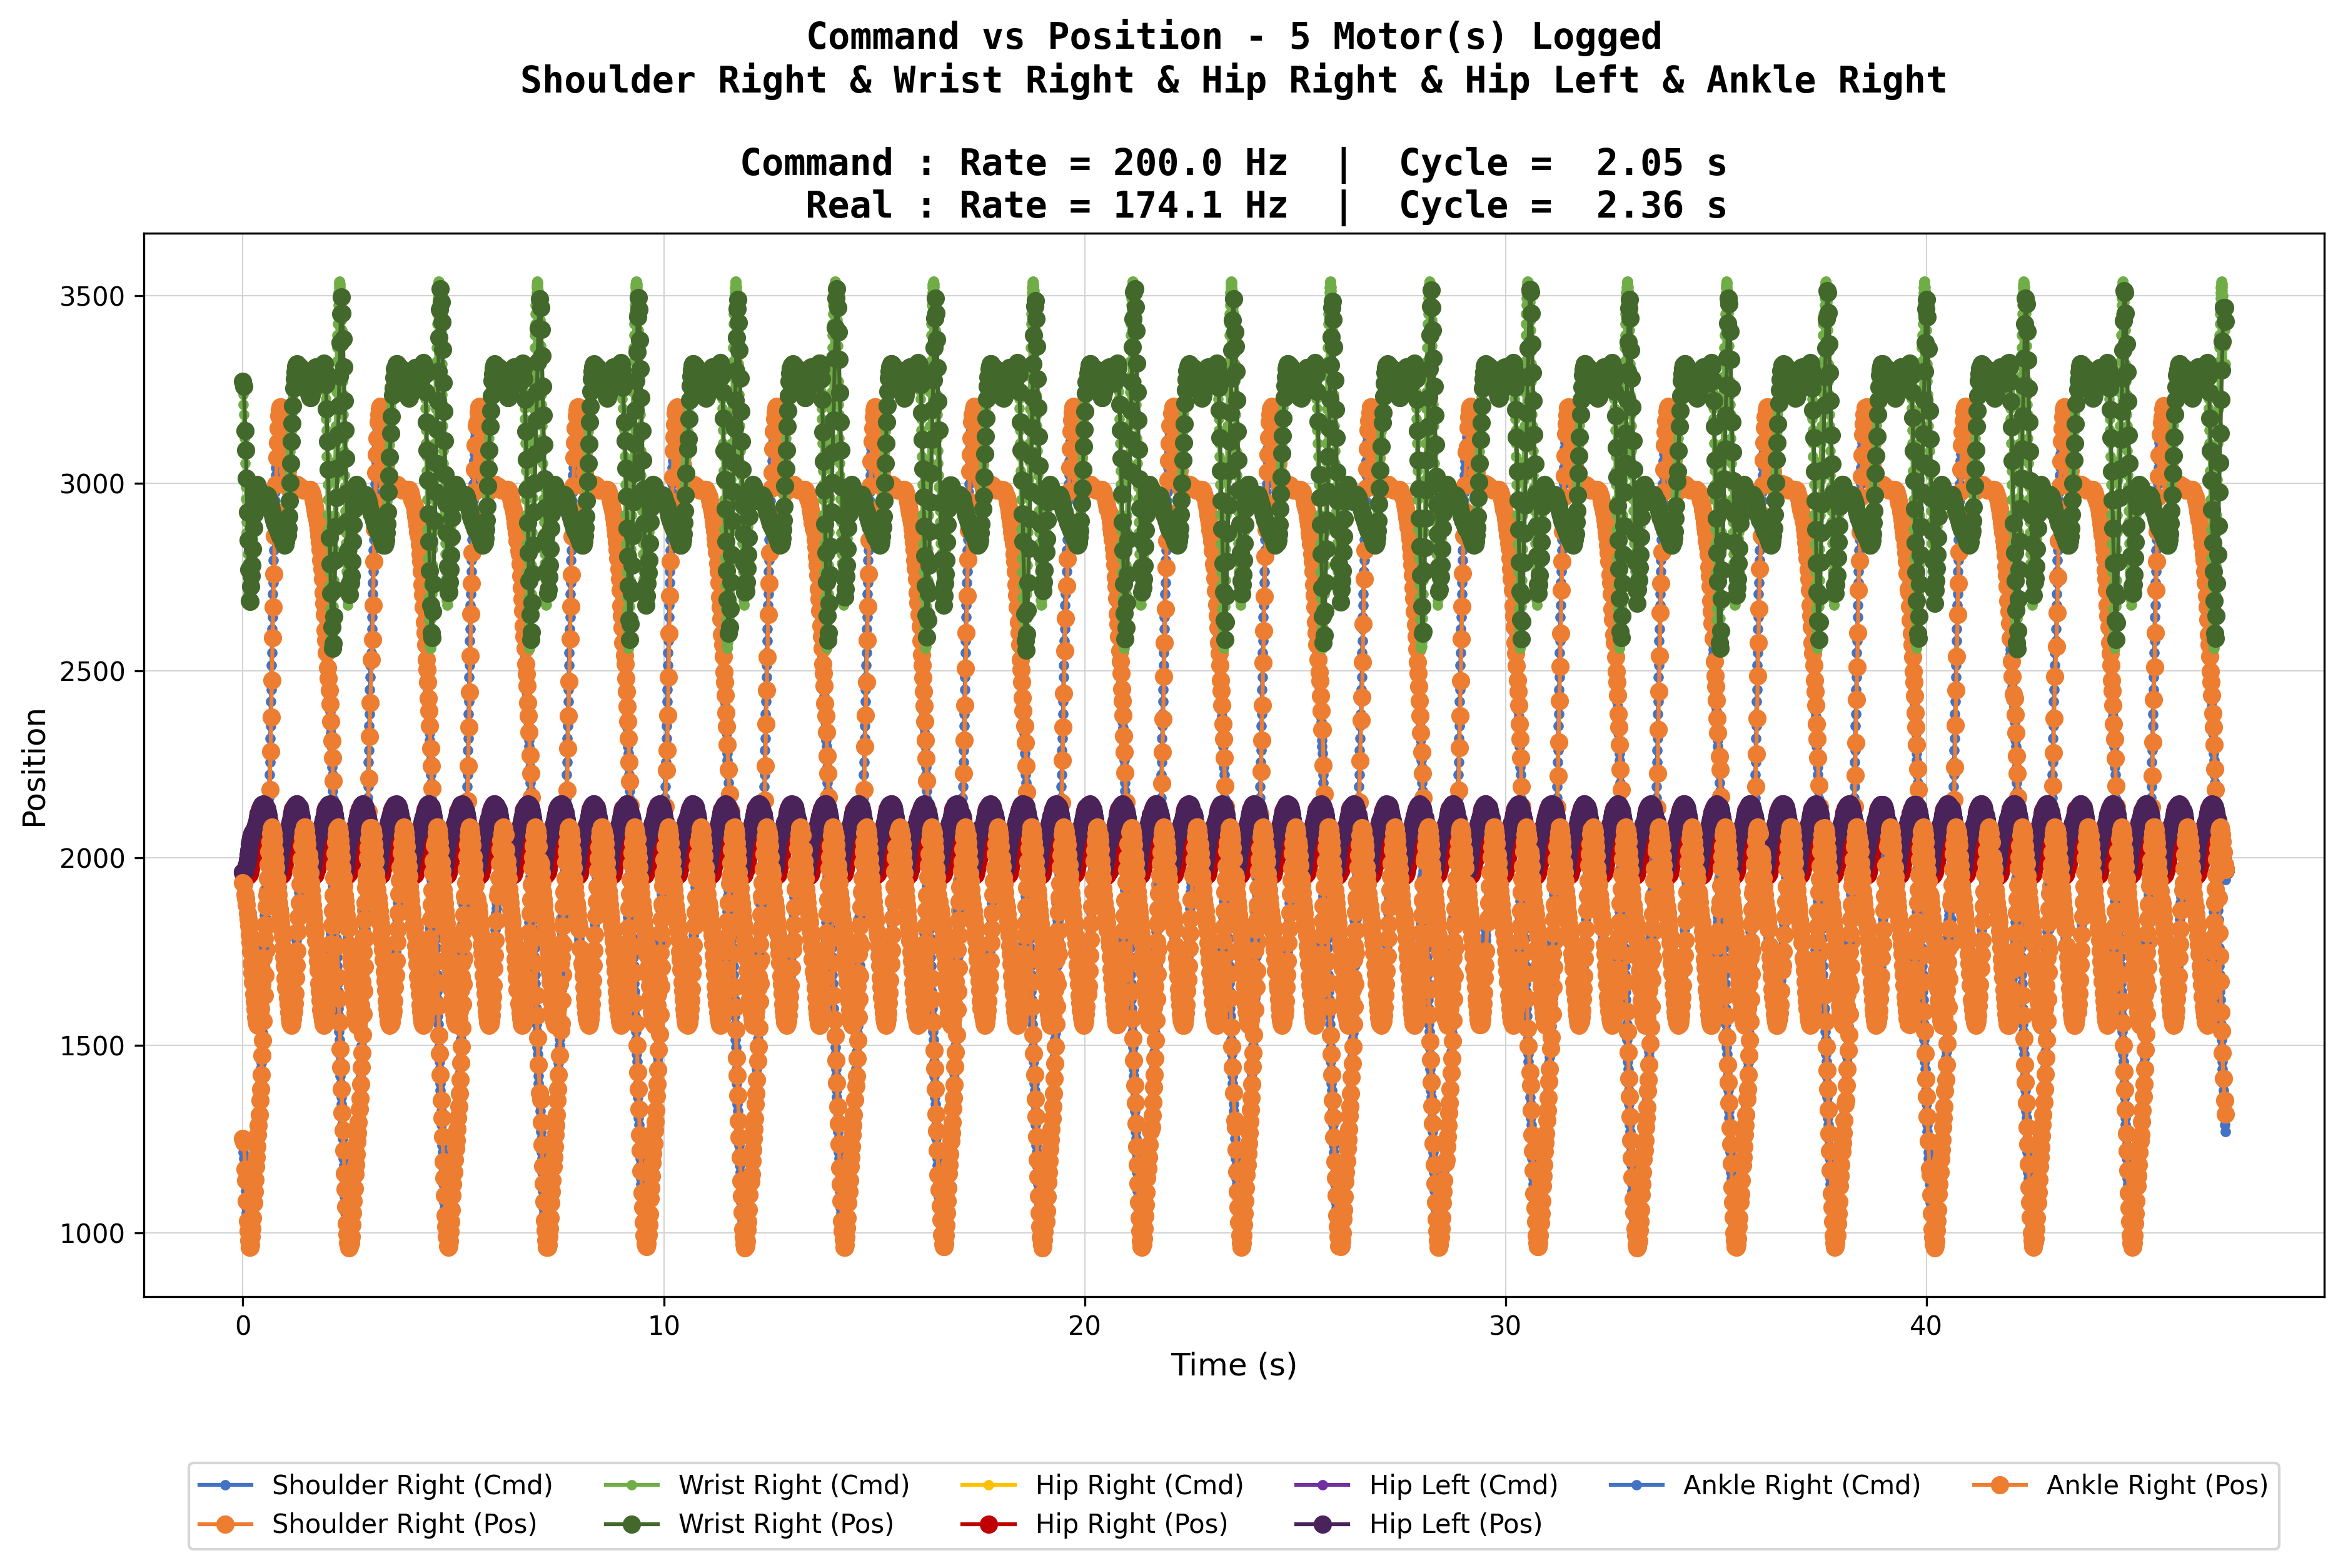
\includegraphics[width=\textwidth]{graphiques/log_5mot_dur4.png}
        \caption{$\sim$47\,s $\rightarrow$ 174.1 Hz.}
    \end{subfigure}
    \caption{Tests at different numbers of cycles at 200\,Hz, $N = 5$.}
    \label{fig:cumulatif}
\end{figure}

\fi

Finally, moving to high throughput does more than improve tracking, in fact, it makes the system's timing behavior \emph{predictable and controllable}. The real control frequency is described by a simple, validated model, with two regimes separated by the threshold $f^\star$, so it can be fixed deterministically at the design stage of a test, by choosing the rate and the number of logged motors. This predictability is nice for the later study of the swimming dynamics to have fine control of the command rate.



\subsection{Test on the SWUMANOID}

With the time-budget model established and validated on the five-motor bench, it remained to test it on the full robot, under real operating conditions. So I carried the campaign into the SWUMANOID itself and its 21 motors to check that the laws found earlier carry over, and to \emph{determine experimentally the optimal parameter set} for the future swimming experiments. As shown in the previous section, logging at 200\,Hz causes saturation when recording multiple motors, while frequencies of 36 or 72\,Hz waste control bandwidth. So 100\,Hz offers the best compromise since its $T_c = 10$\,ms budget is wide enough to absorb the reading of many motors without collapsing the rate, while keeping a high control frequency. So keeping 100\,Hz, a cycle time of 2.05\,s and sampling every 3 frames, I first raised the number of logged motors progressively as we can see in the figure~\ref{fig:swum_scaling_part1} and \ref{fig:swum_scaling_part2} :

\begin{figure}[H]
    \centering
    \begin{subfigure}[b]{0.48\textwidth}
        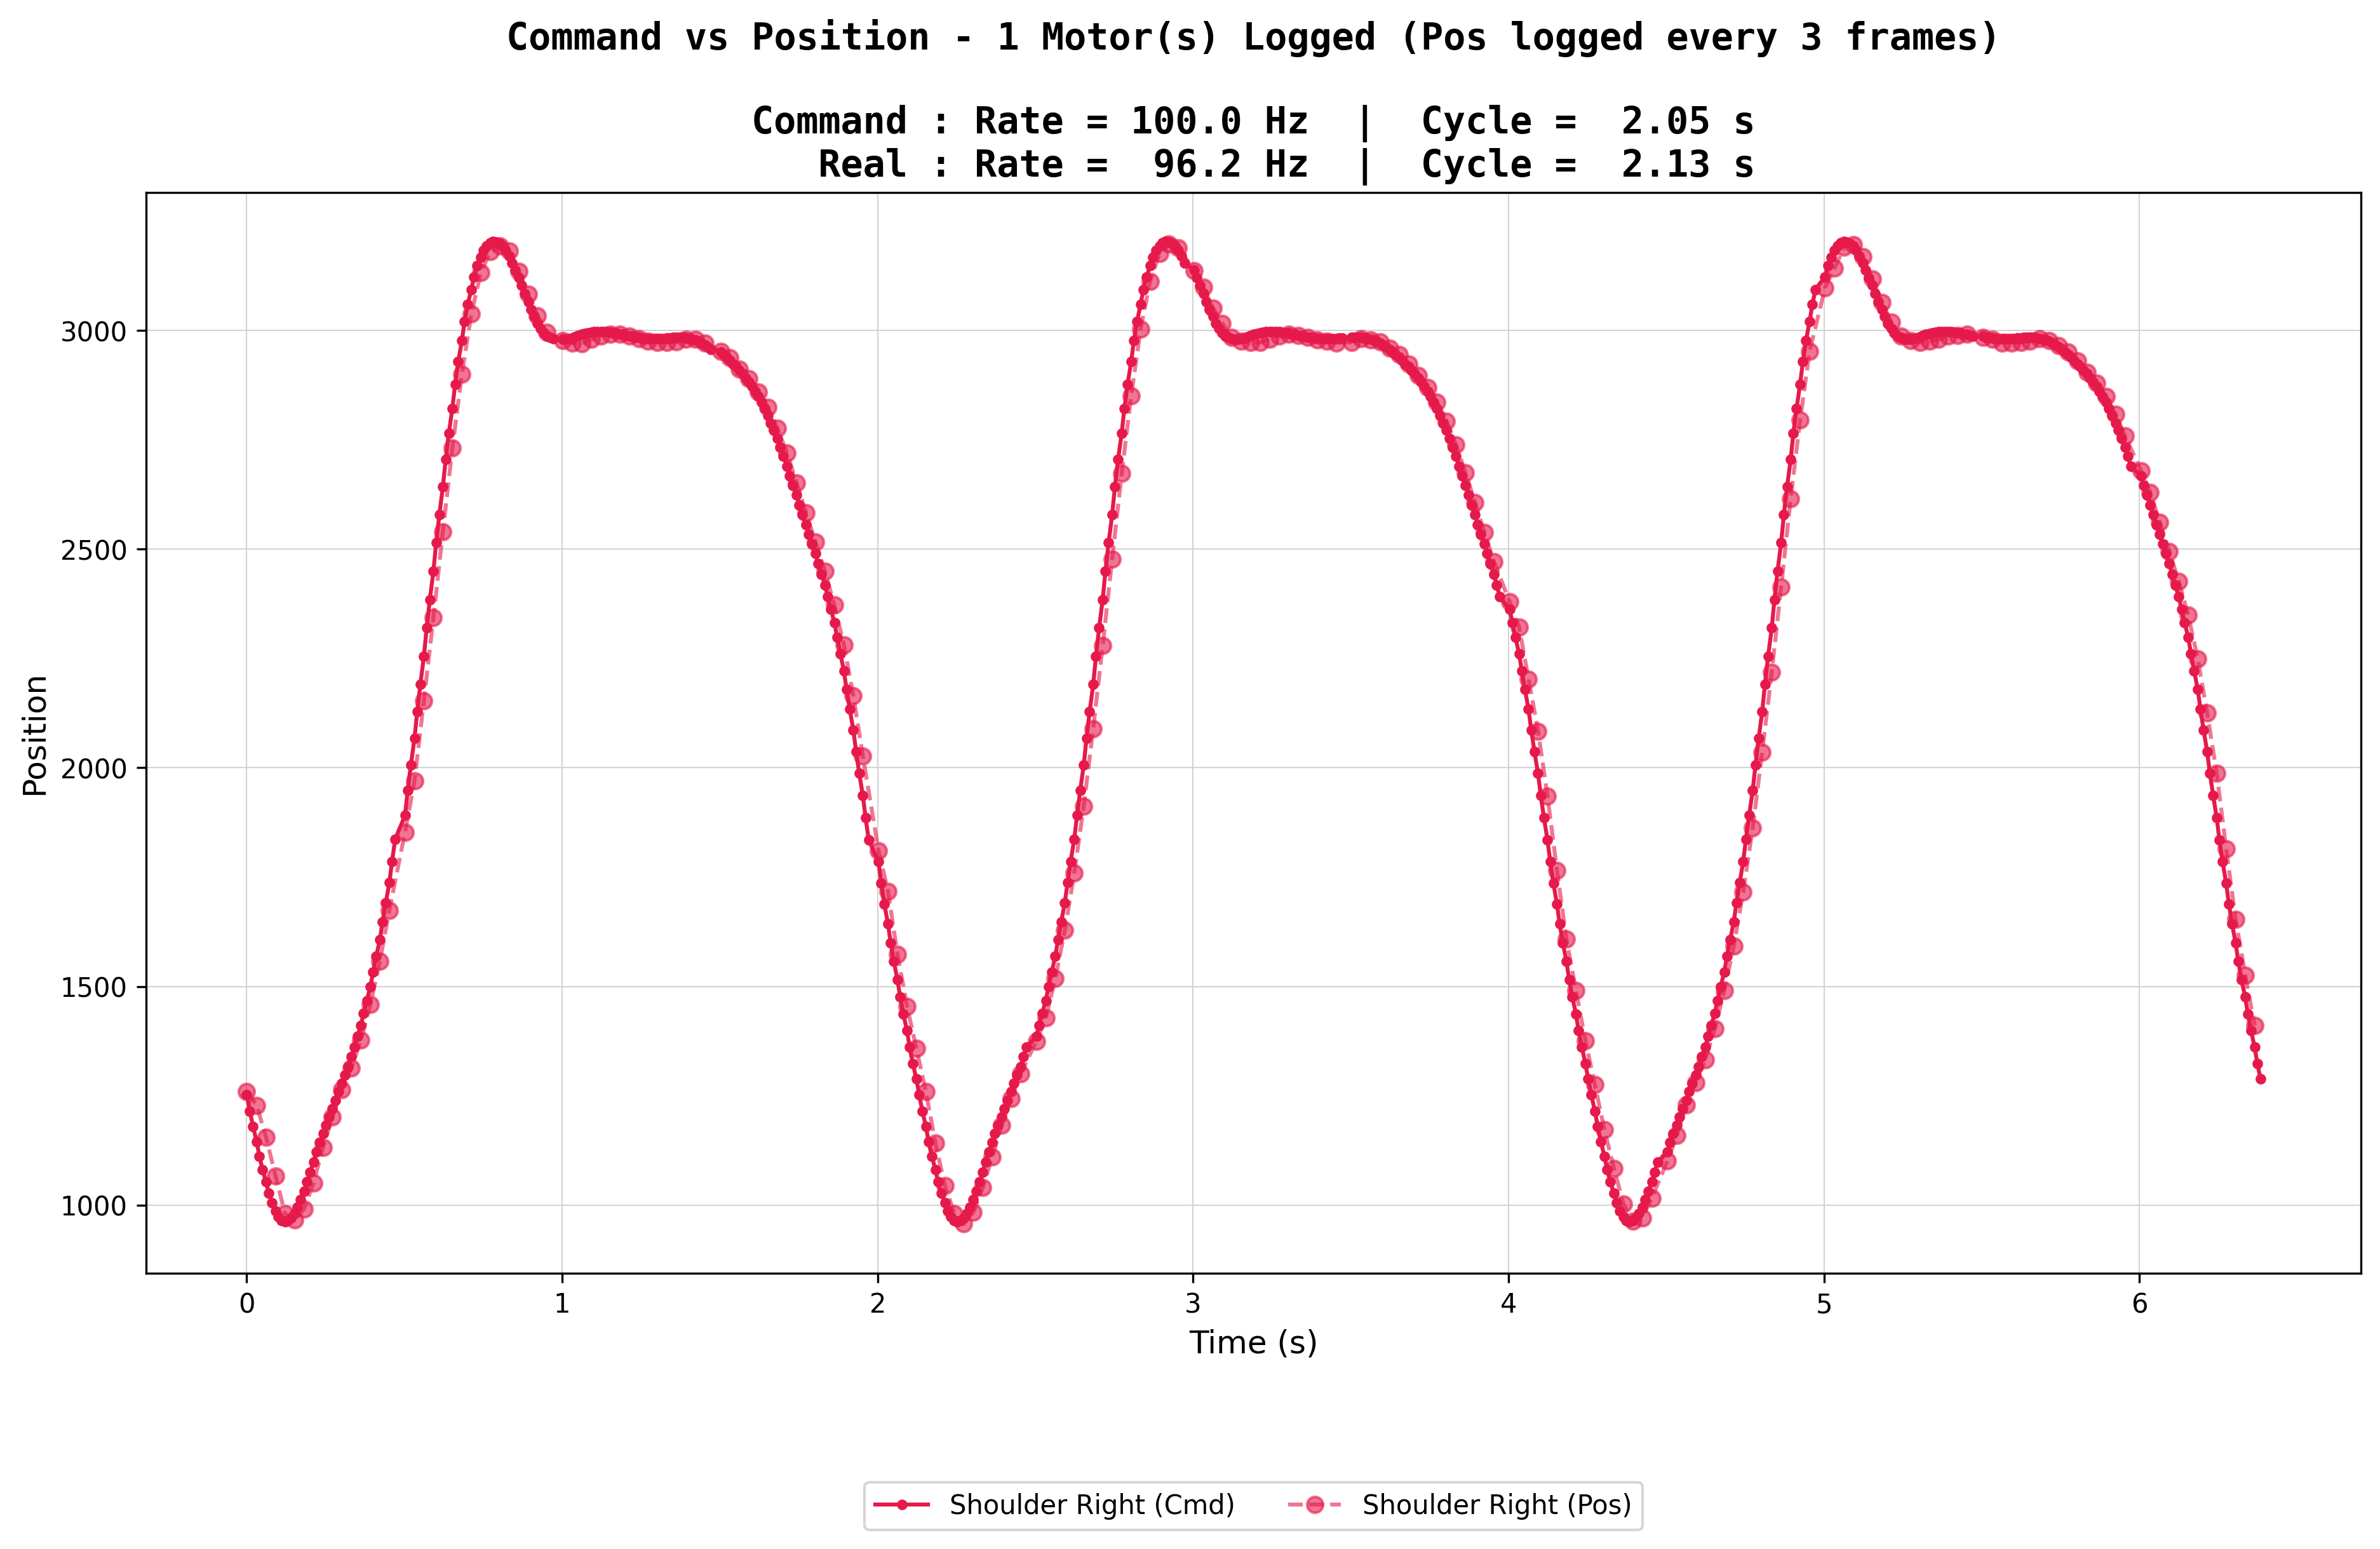
\includegraphics[width=\textwidth]{graphiques_swumanoid/swum_1mot_3f.png}
        \caption{1 motor $\rightarrow$ 96.2 Hz.}
    \end{subfigure}
    \hfill
    \begin{subfigure}[b]{0.48\textwidth}
        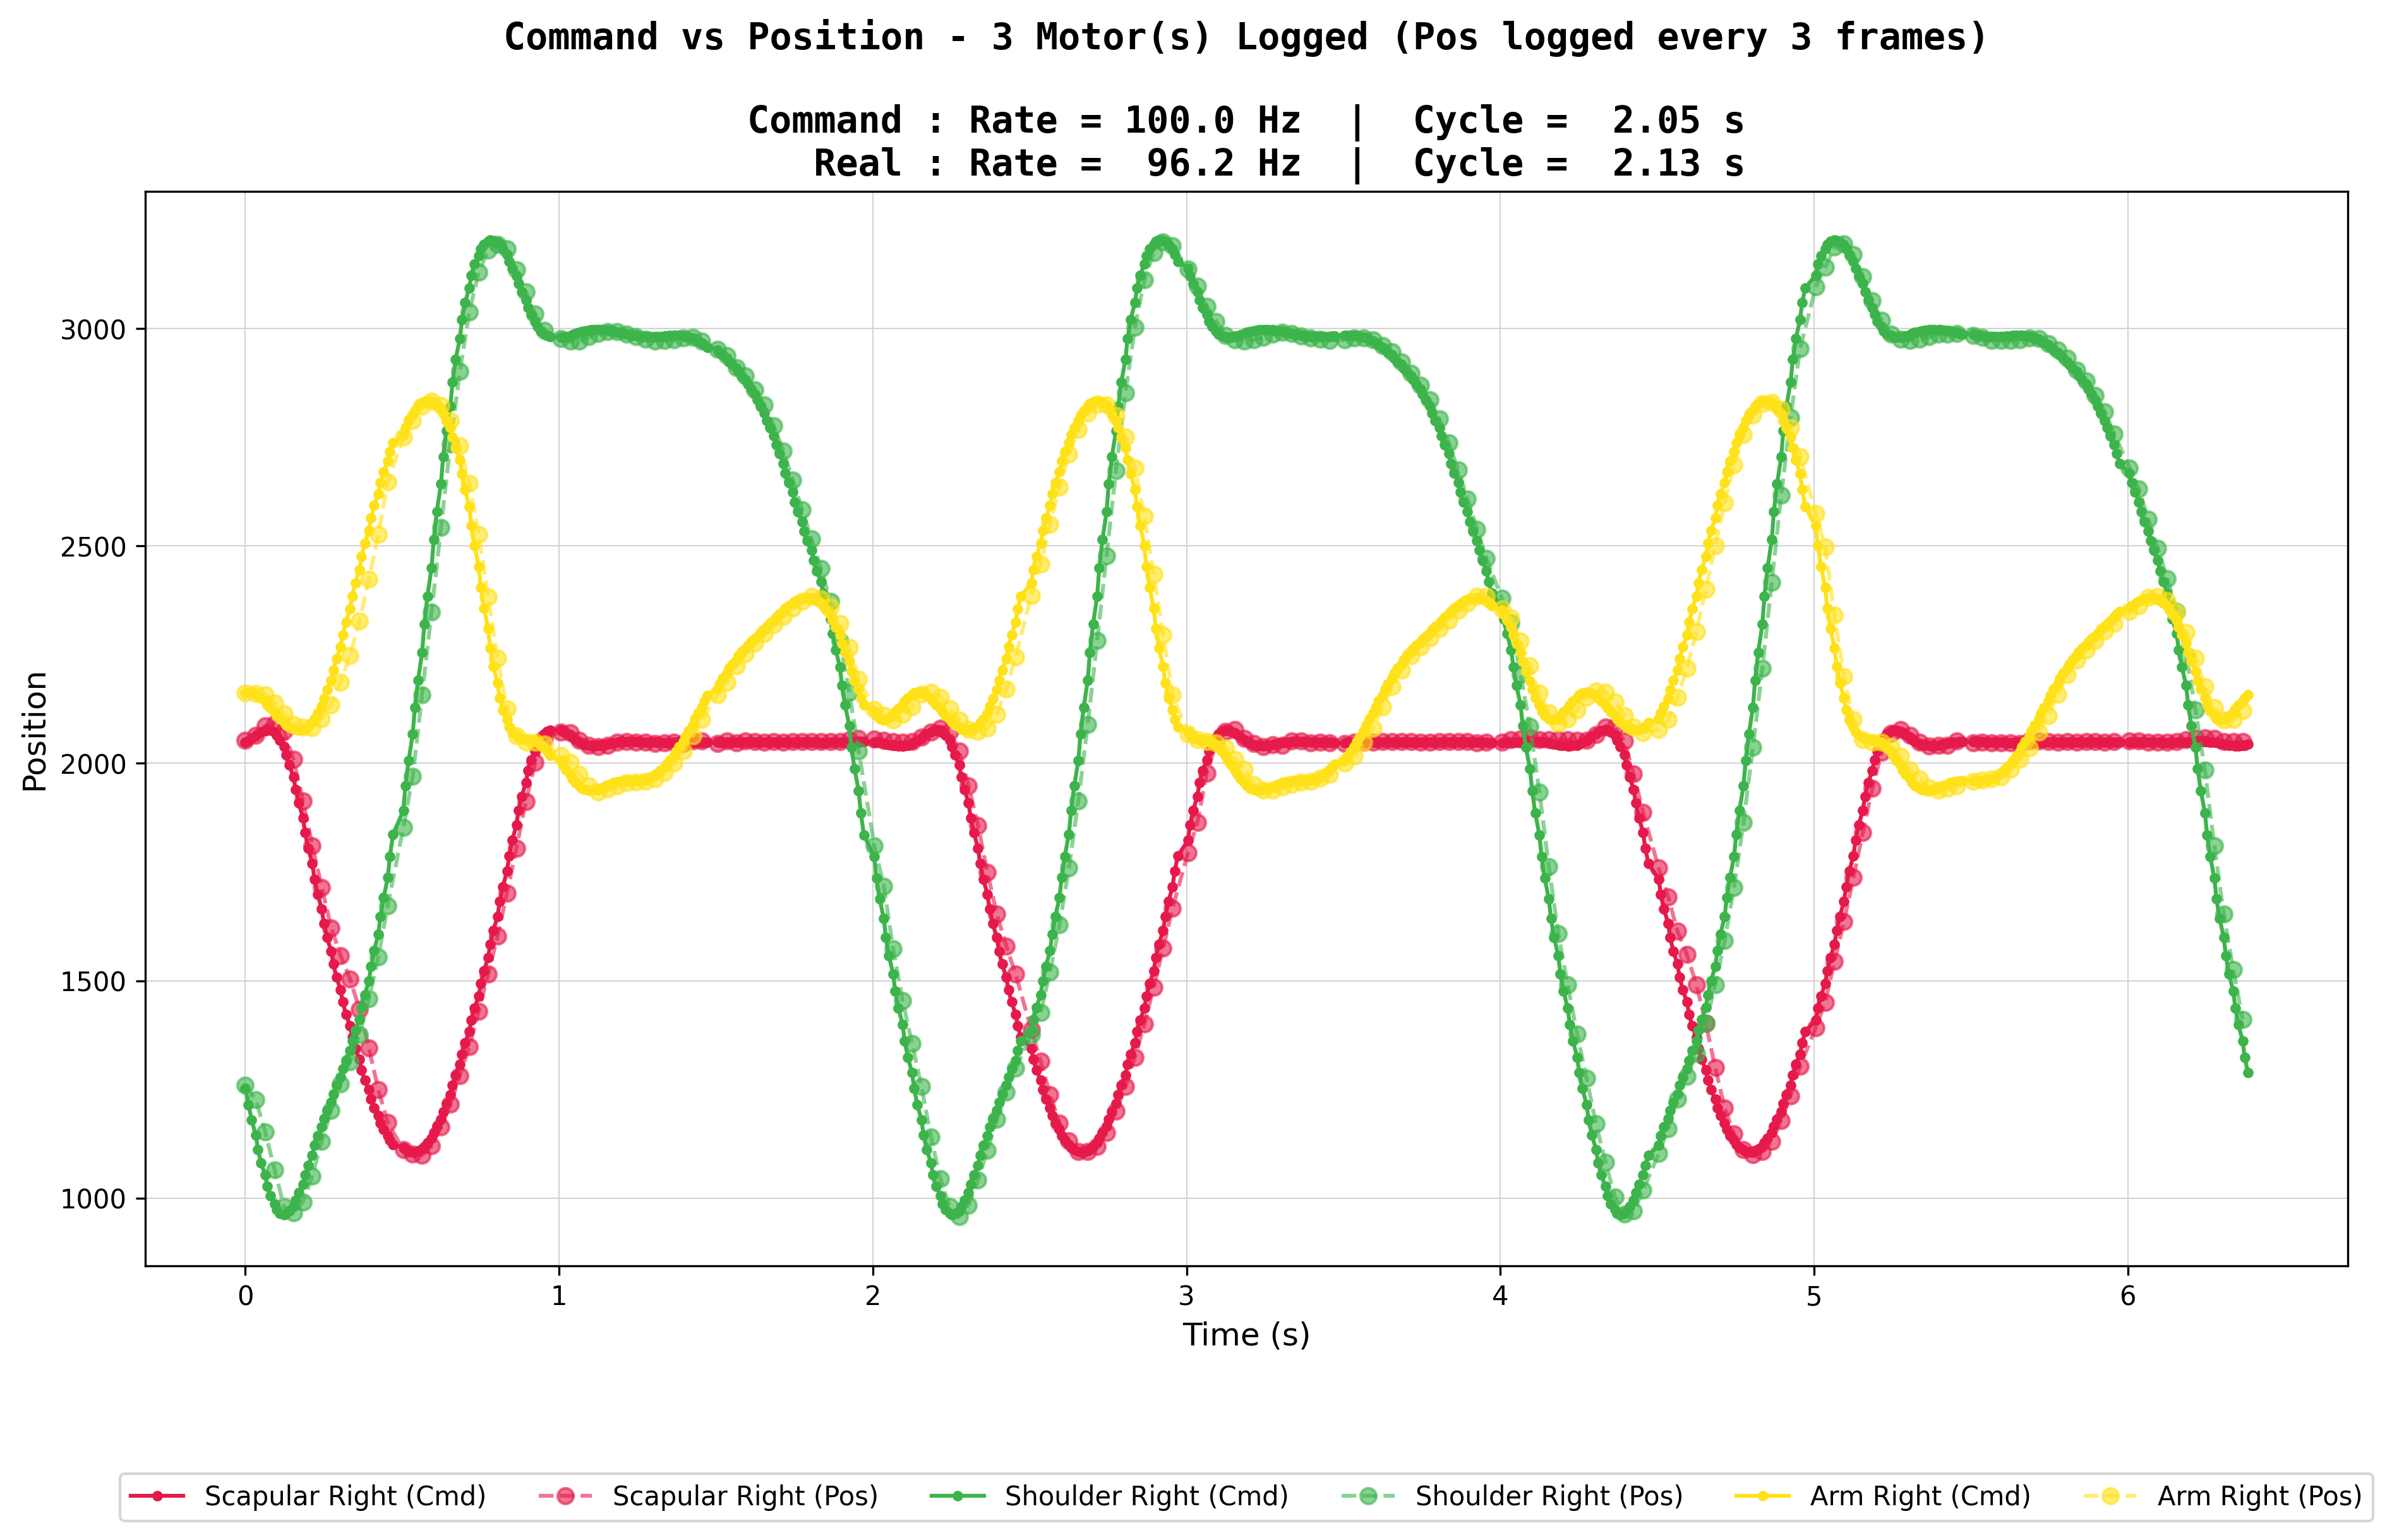
\includegraphics[width=\textwidth]{graphiques_swumanoid/swum_3mot_3f.png}
        \caption{3 motors $\rightarrow$ 96.2 Hz.}
    \end{subfigure}
    \caption{Tests of the number of logged motors on the SWUMANOID (1 and 3 motors)}
    \label{fig:swum_scaling_part1}
\end{figure}

\begin{figure}[H]
    \centering
    \begin{subfigure}[b]{0.48\textwidth}
        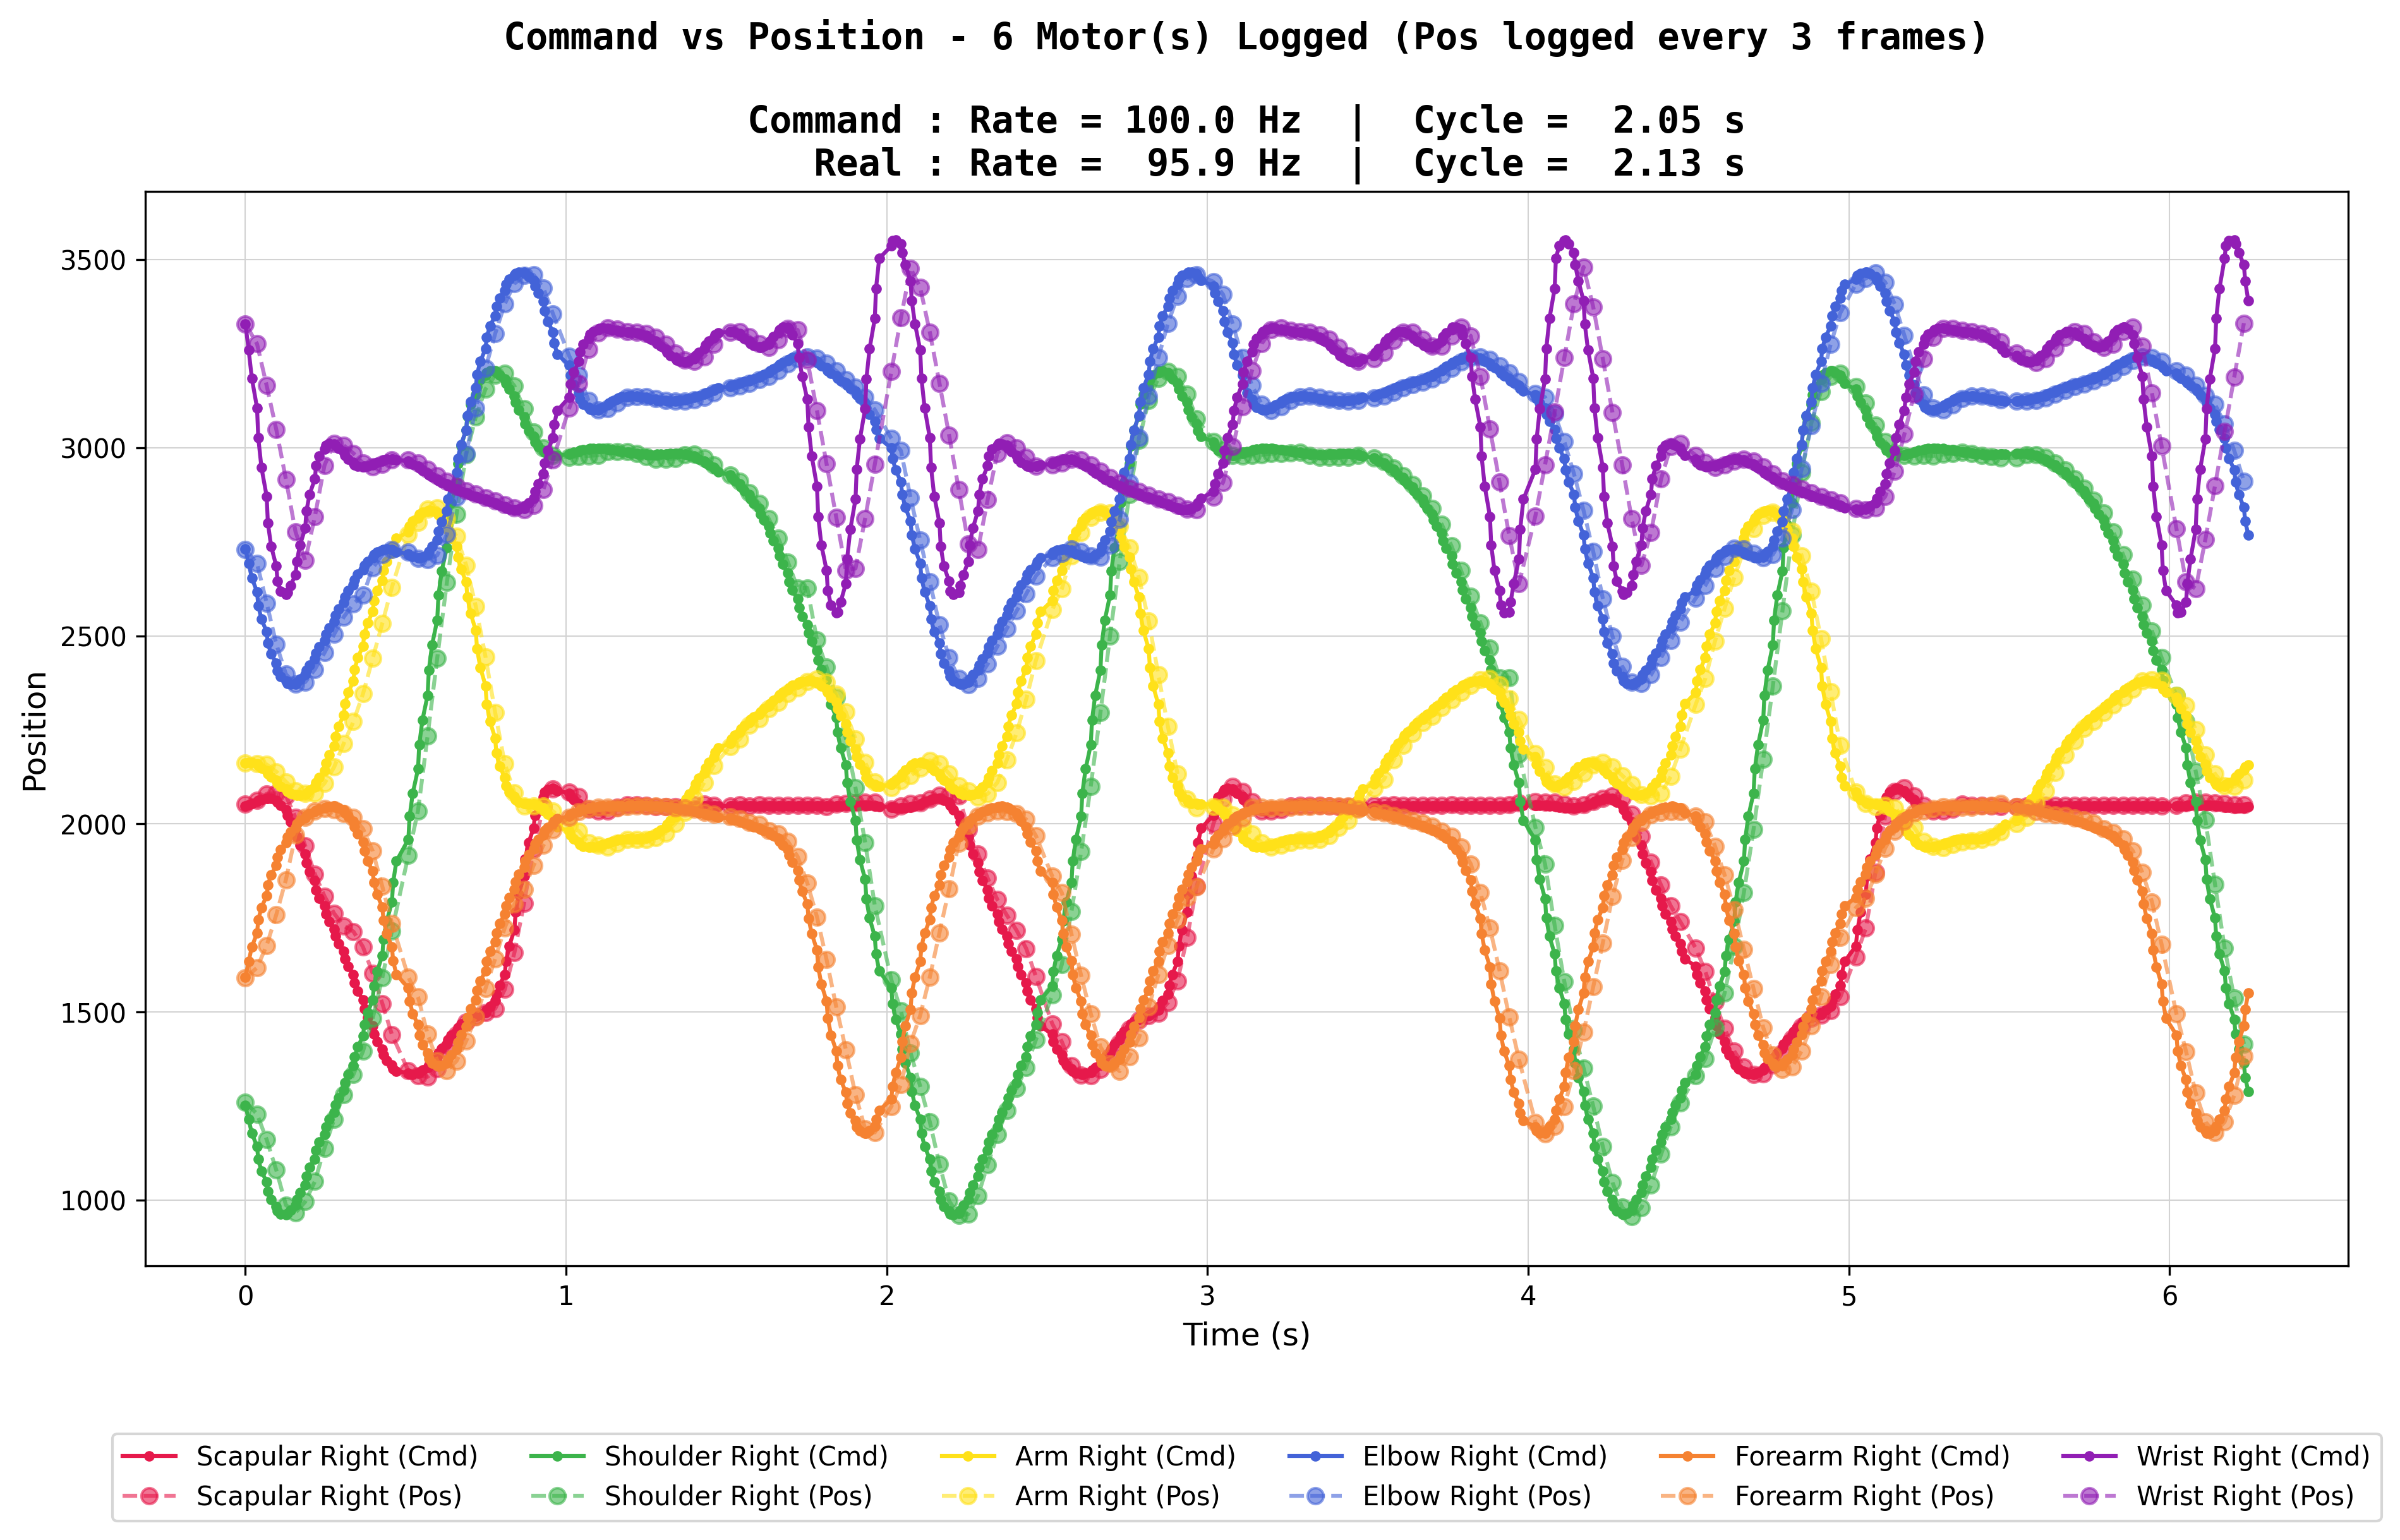
\includegraphics[width=\textwidth]{graphiques_swumanoid/swum_6mot_3f.png}
        \caption{6 motors $\rightarrow$ 95.9 Hz.}
    \end{subfigure}
    \hfill
    \begin{subfigure}[b]{0.48\textwidth}
        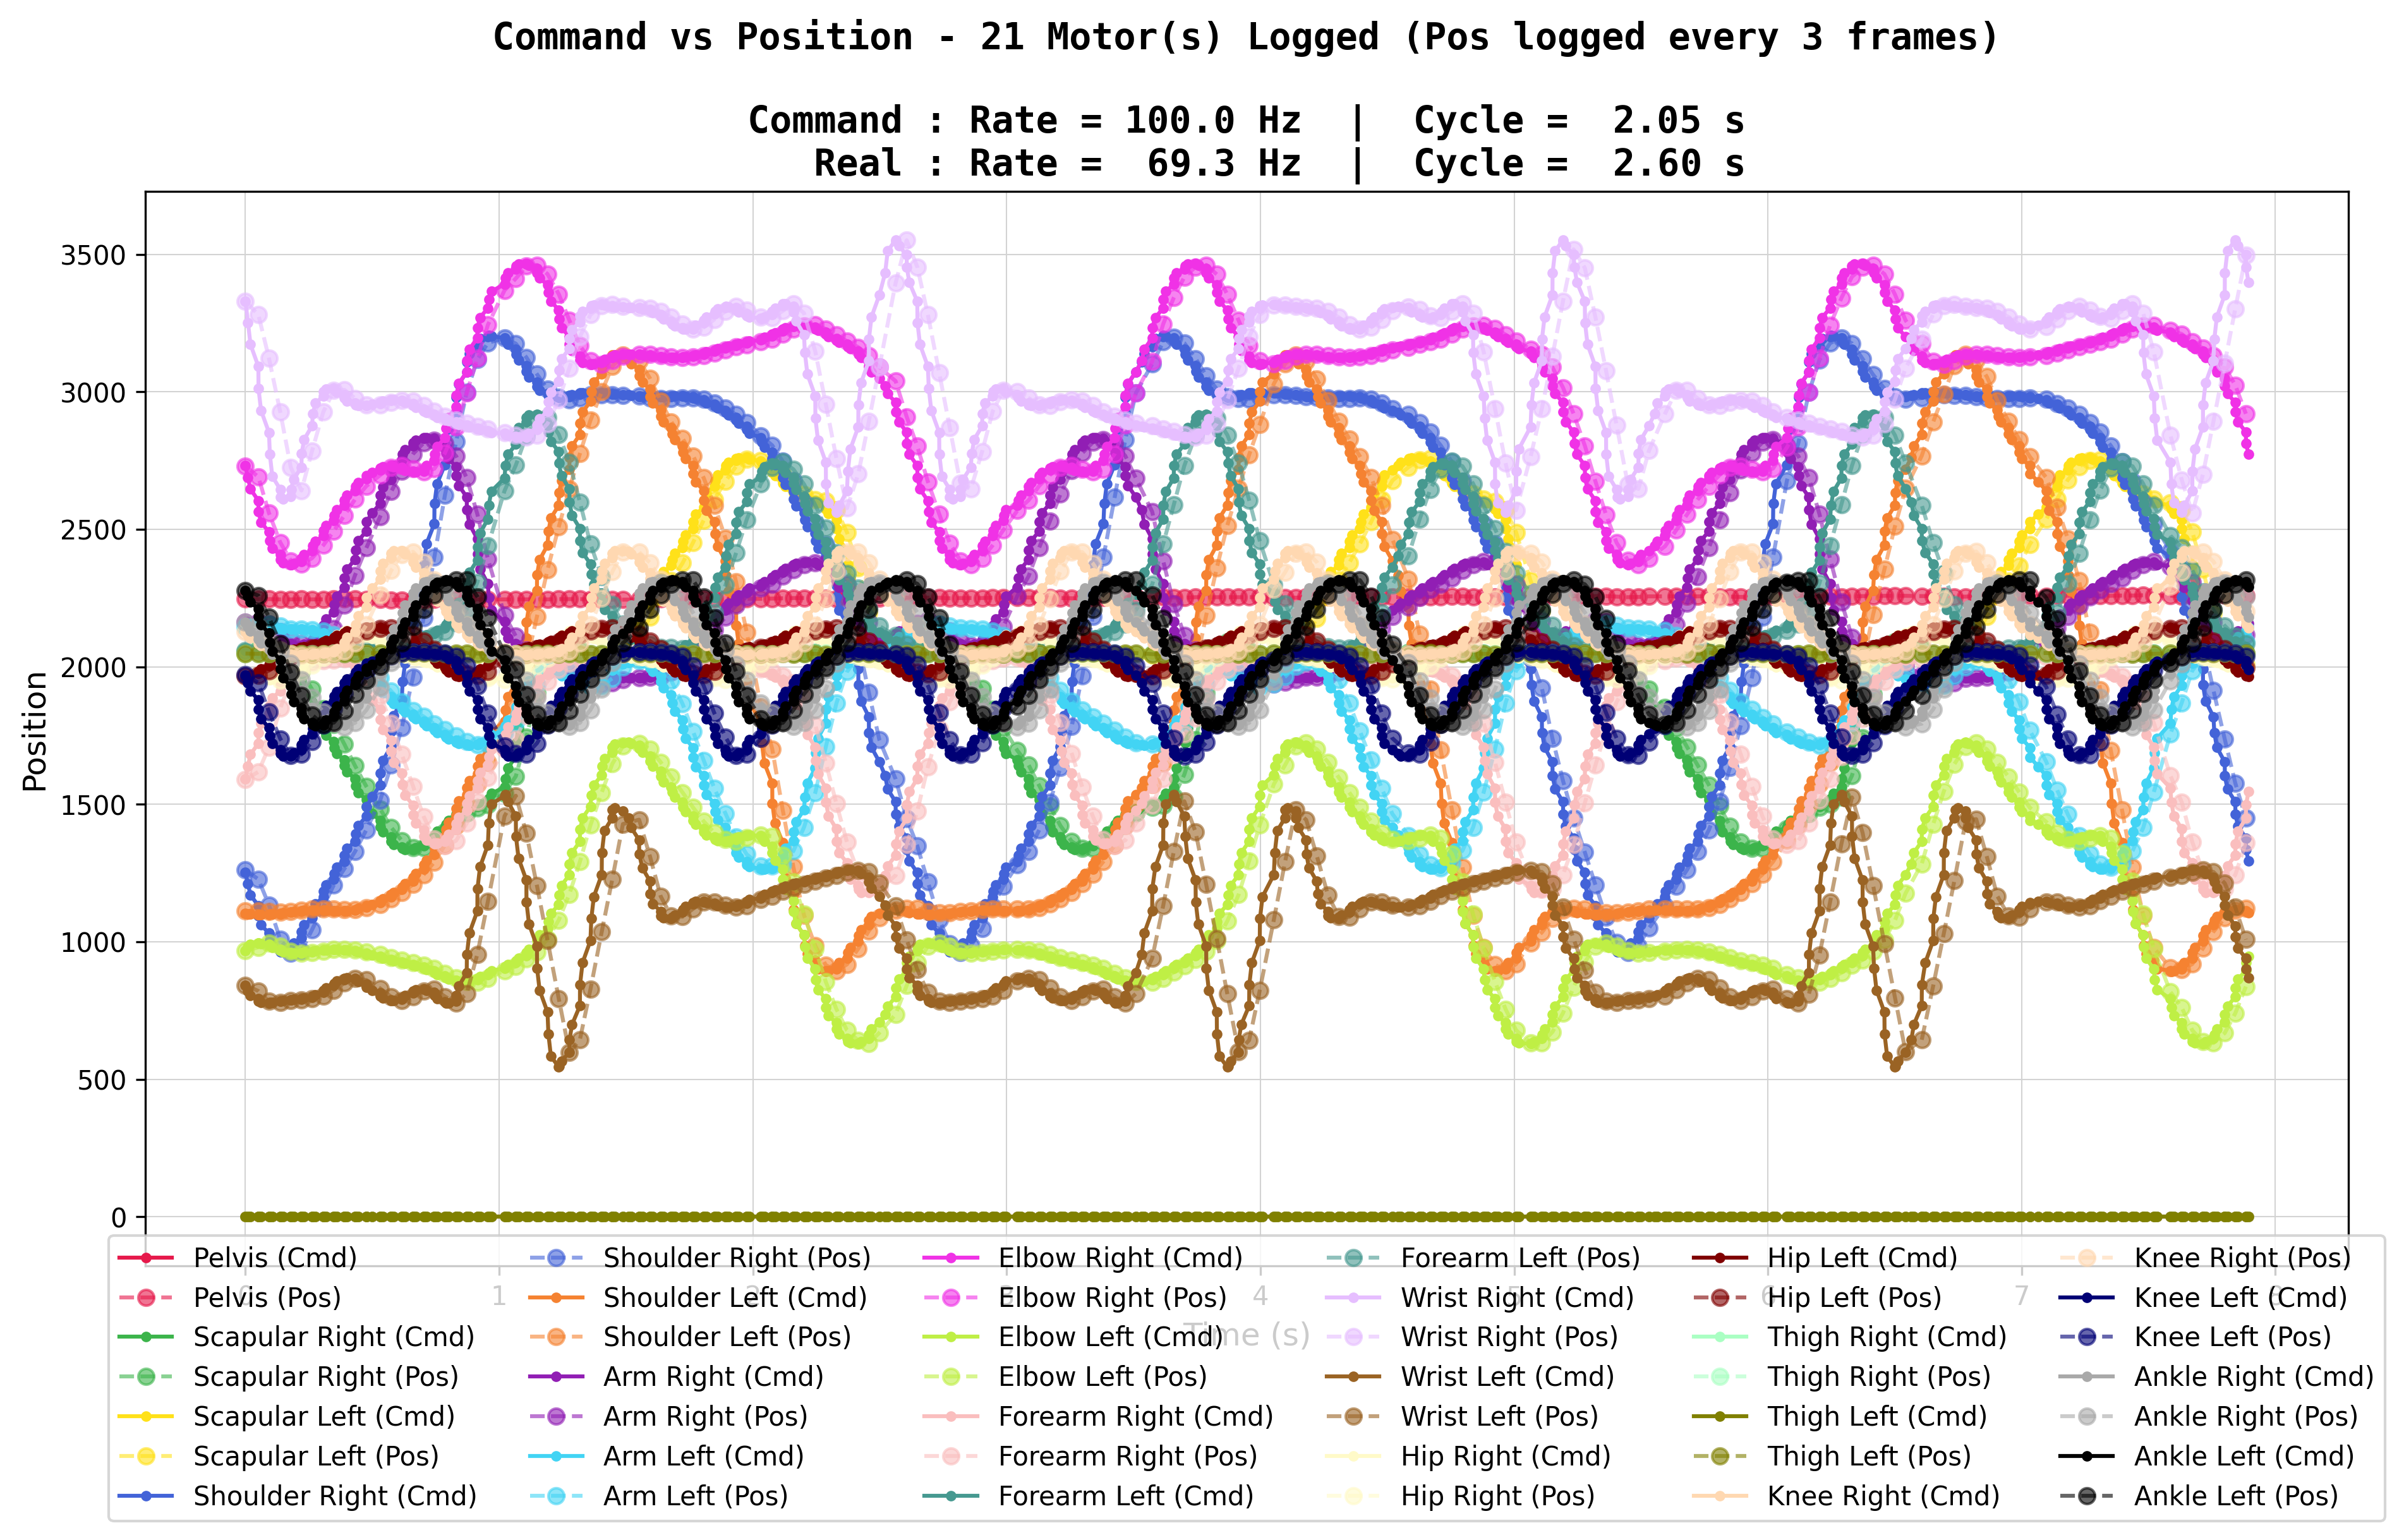
\includegraphics[width=\textwidth]{graphiques_swumanoid/swum_21mot_3f.png}
        \caption{21 motors $\rightarrow$ 69.3 Hz (real cycle 2.60\,s).}
        \label{fig:swum_21_3f}
    \end{subfigure}
    \caption{Tests of the number of logged motors on the SWUMANOID (6 and 21 motors)}
    \label{fig:swum_scaling_part2}
\end{figure}

\iffalse
\begin{figure}[H]
    \centering
    \begin{subfigure}[b]{0.48\textwidth}
        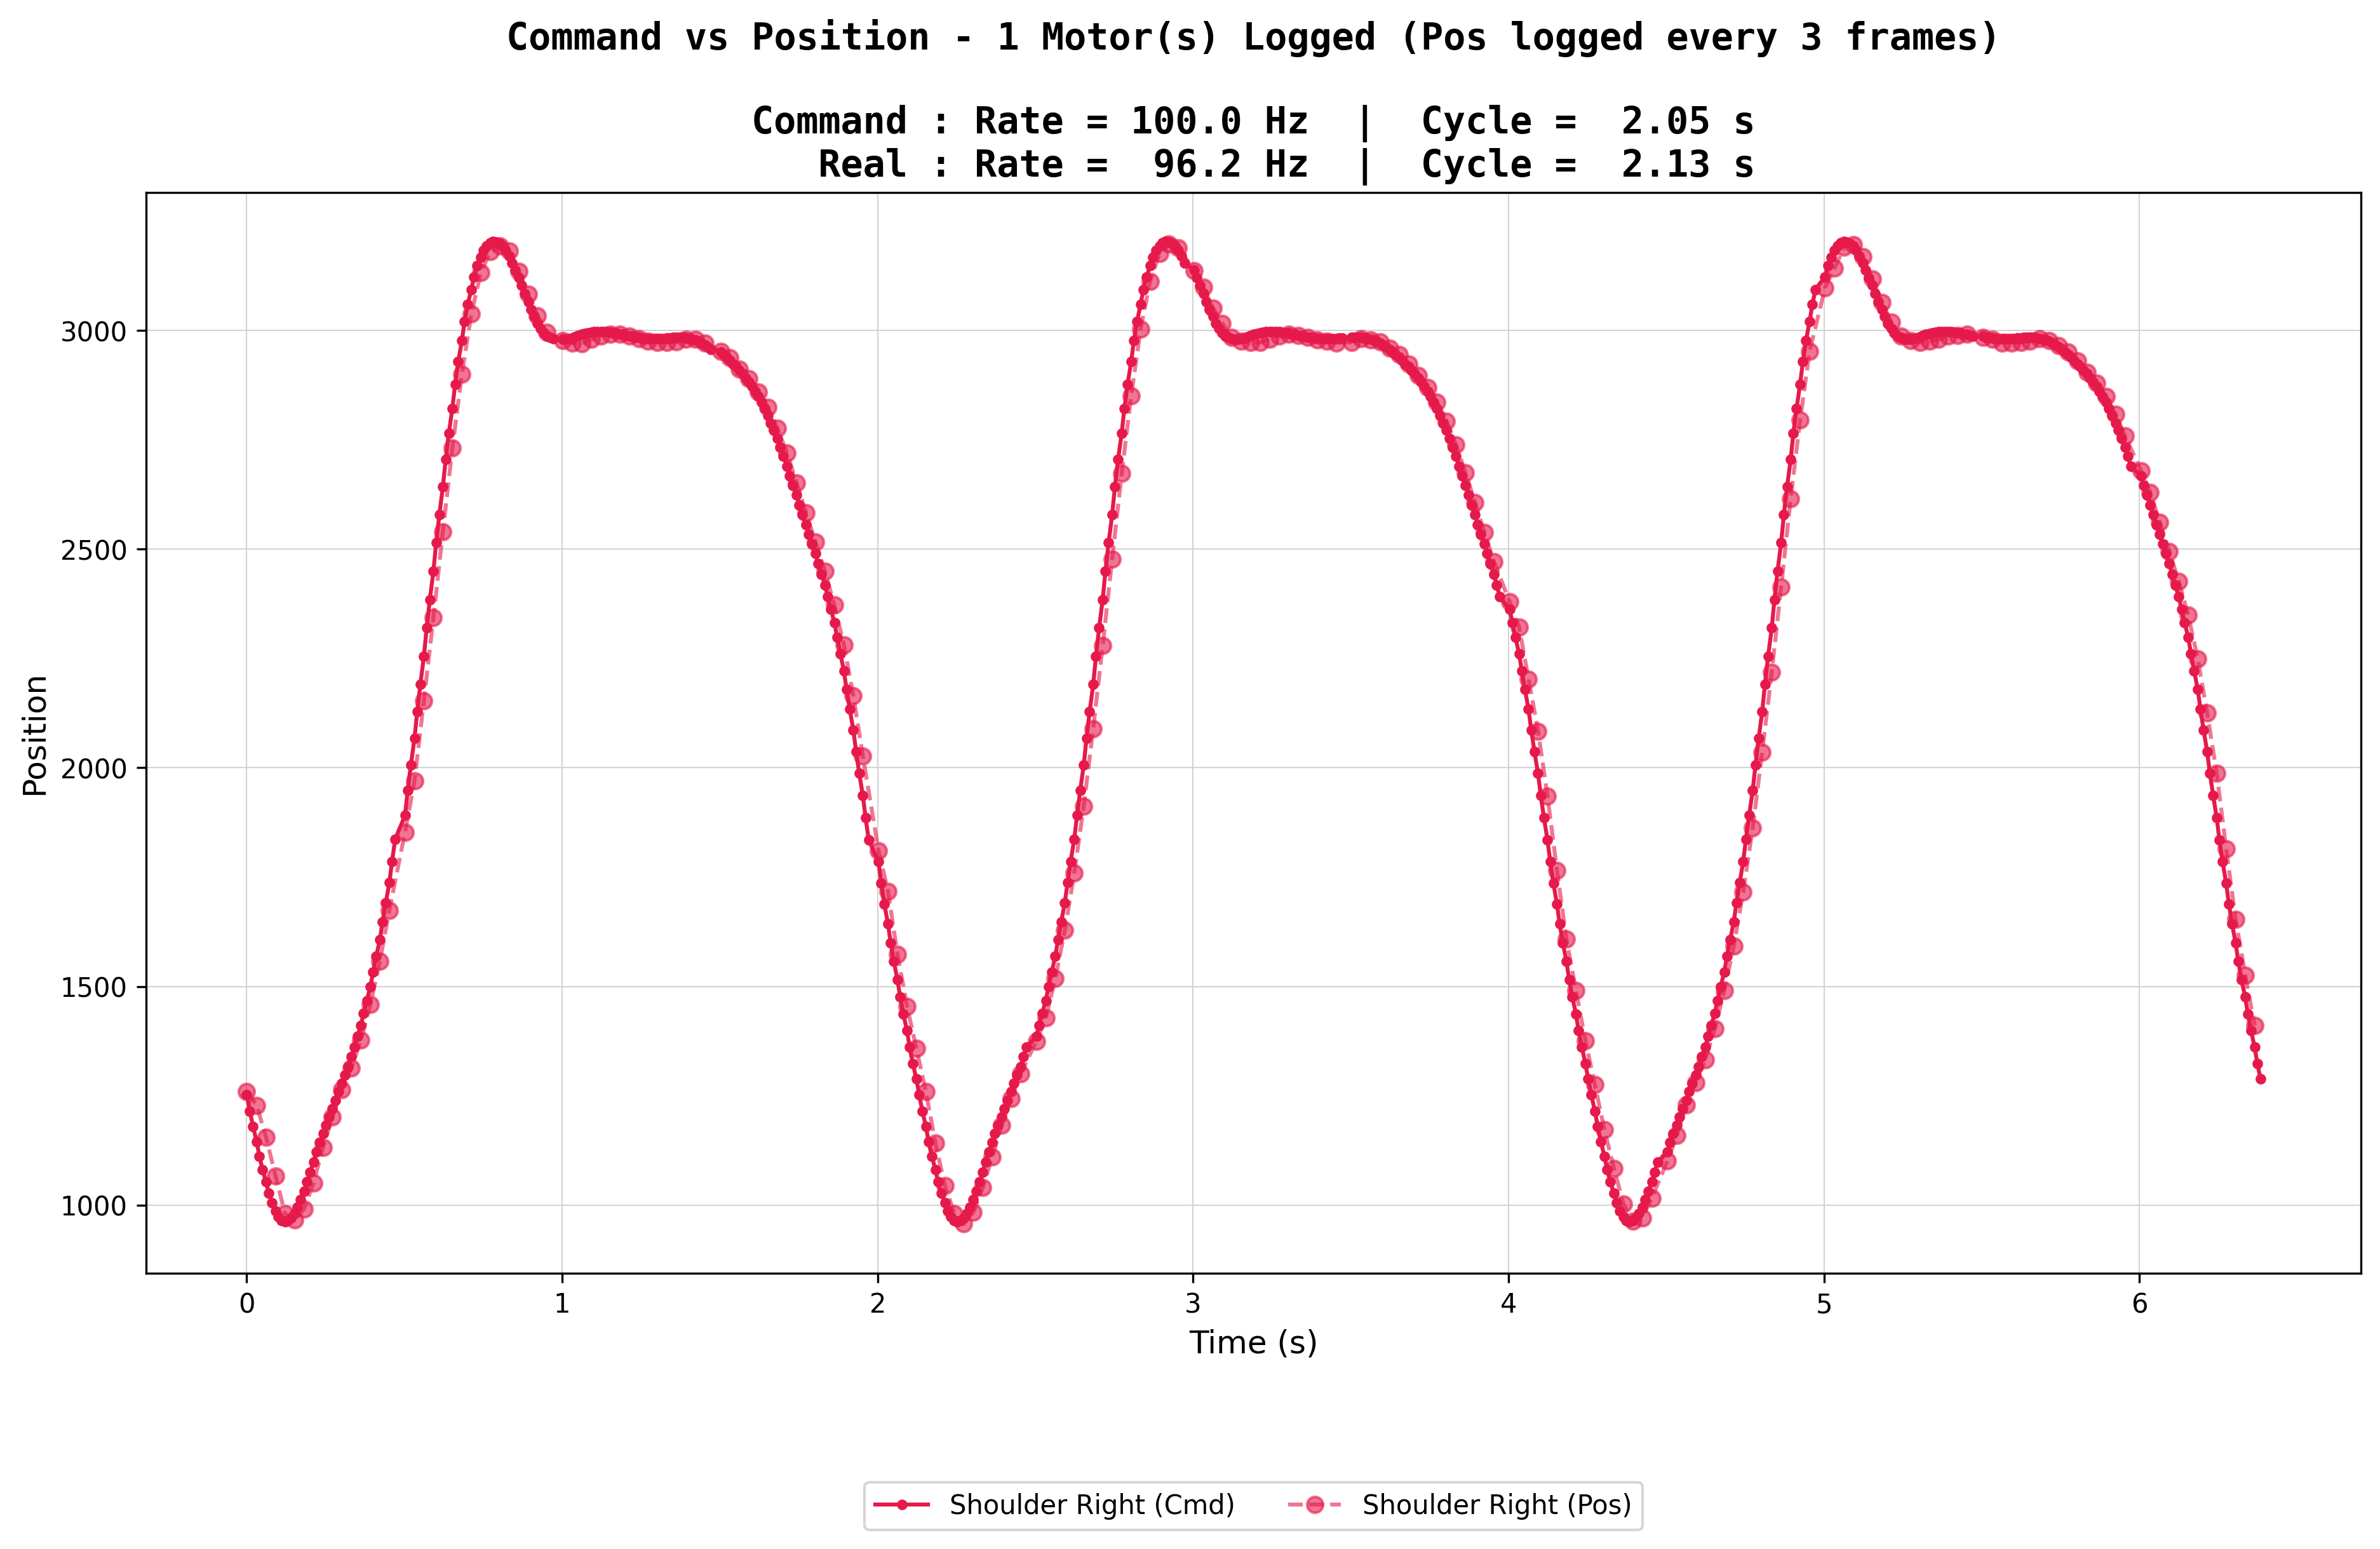
\includegraphics[width=\textwidth]{graphiques_swumanoid/swum_1mot_3f.png}
        \caption{1 motor $\rightarrow$ 96.2 Hz.}
    \end{subfigure}
    \hfill
    \begin{subfigure}[b]{0.48\textwidth}
        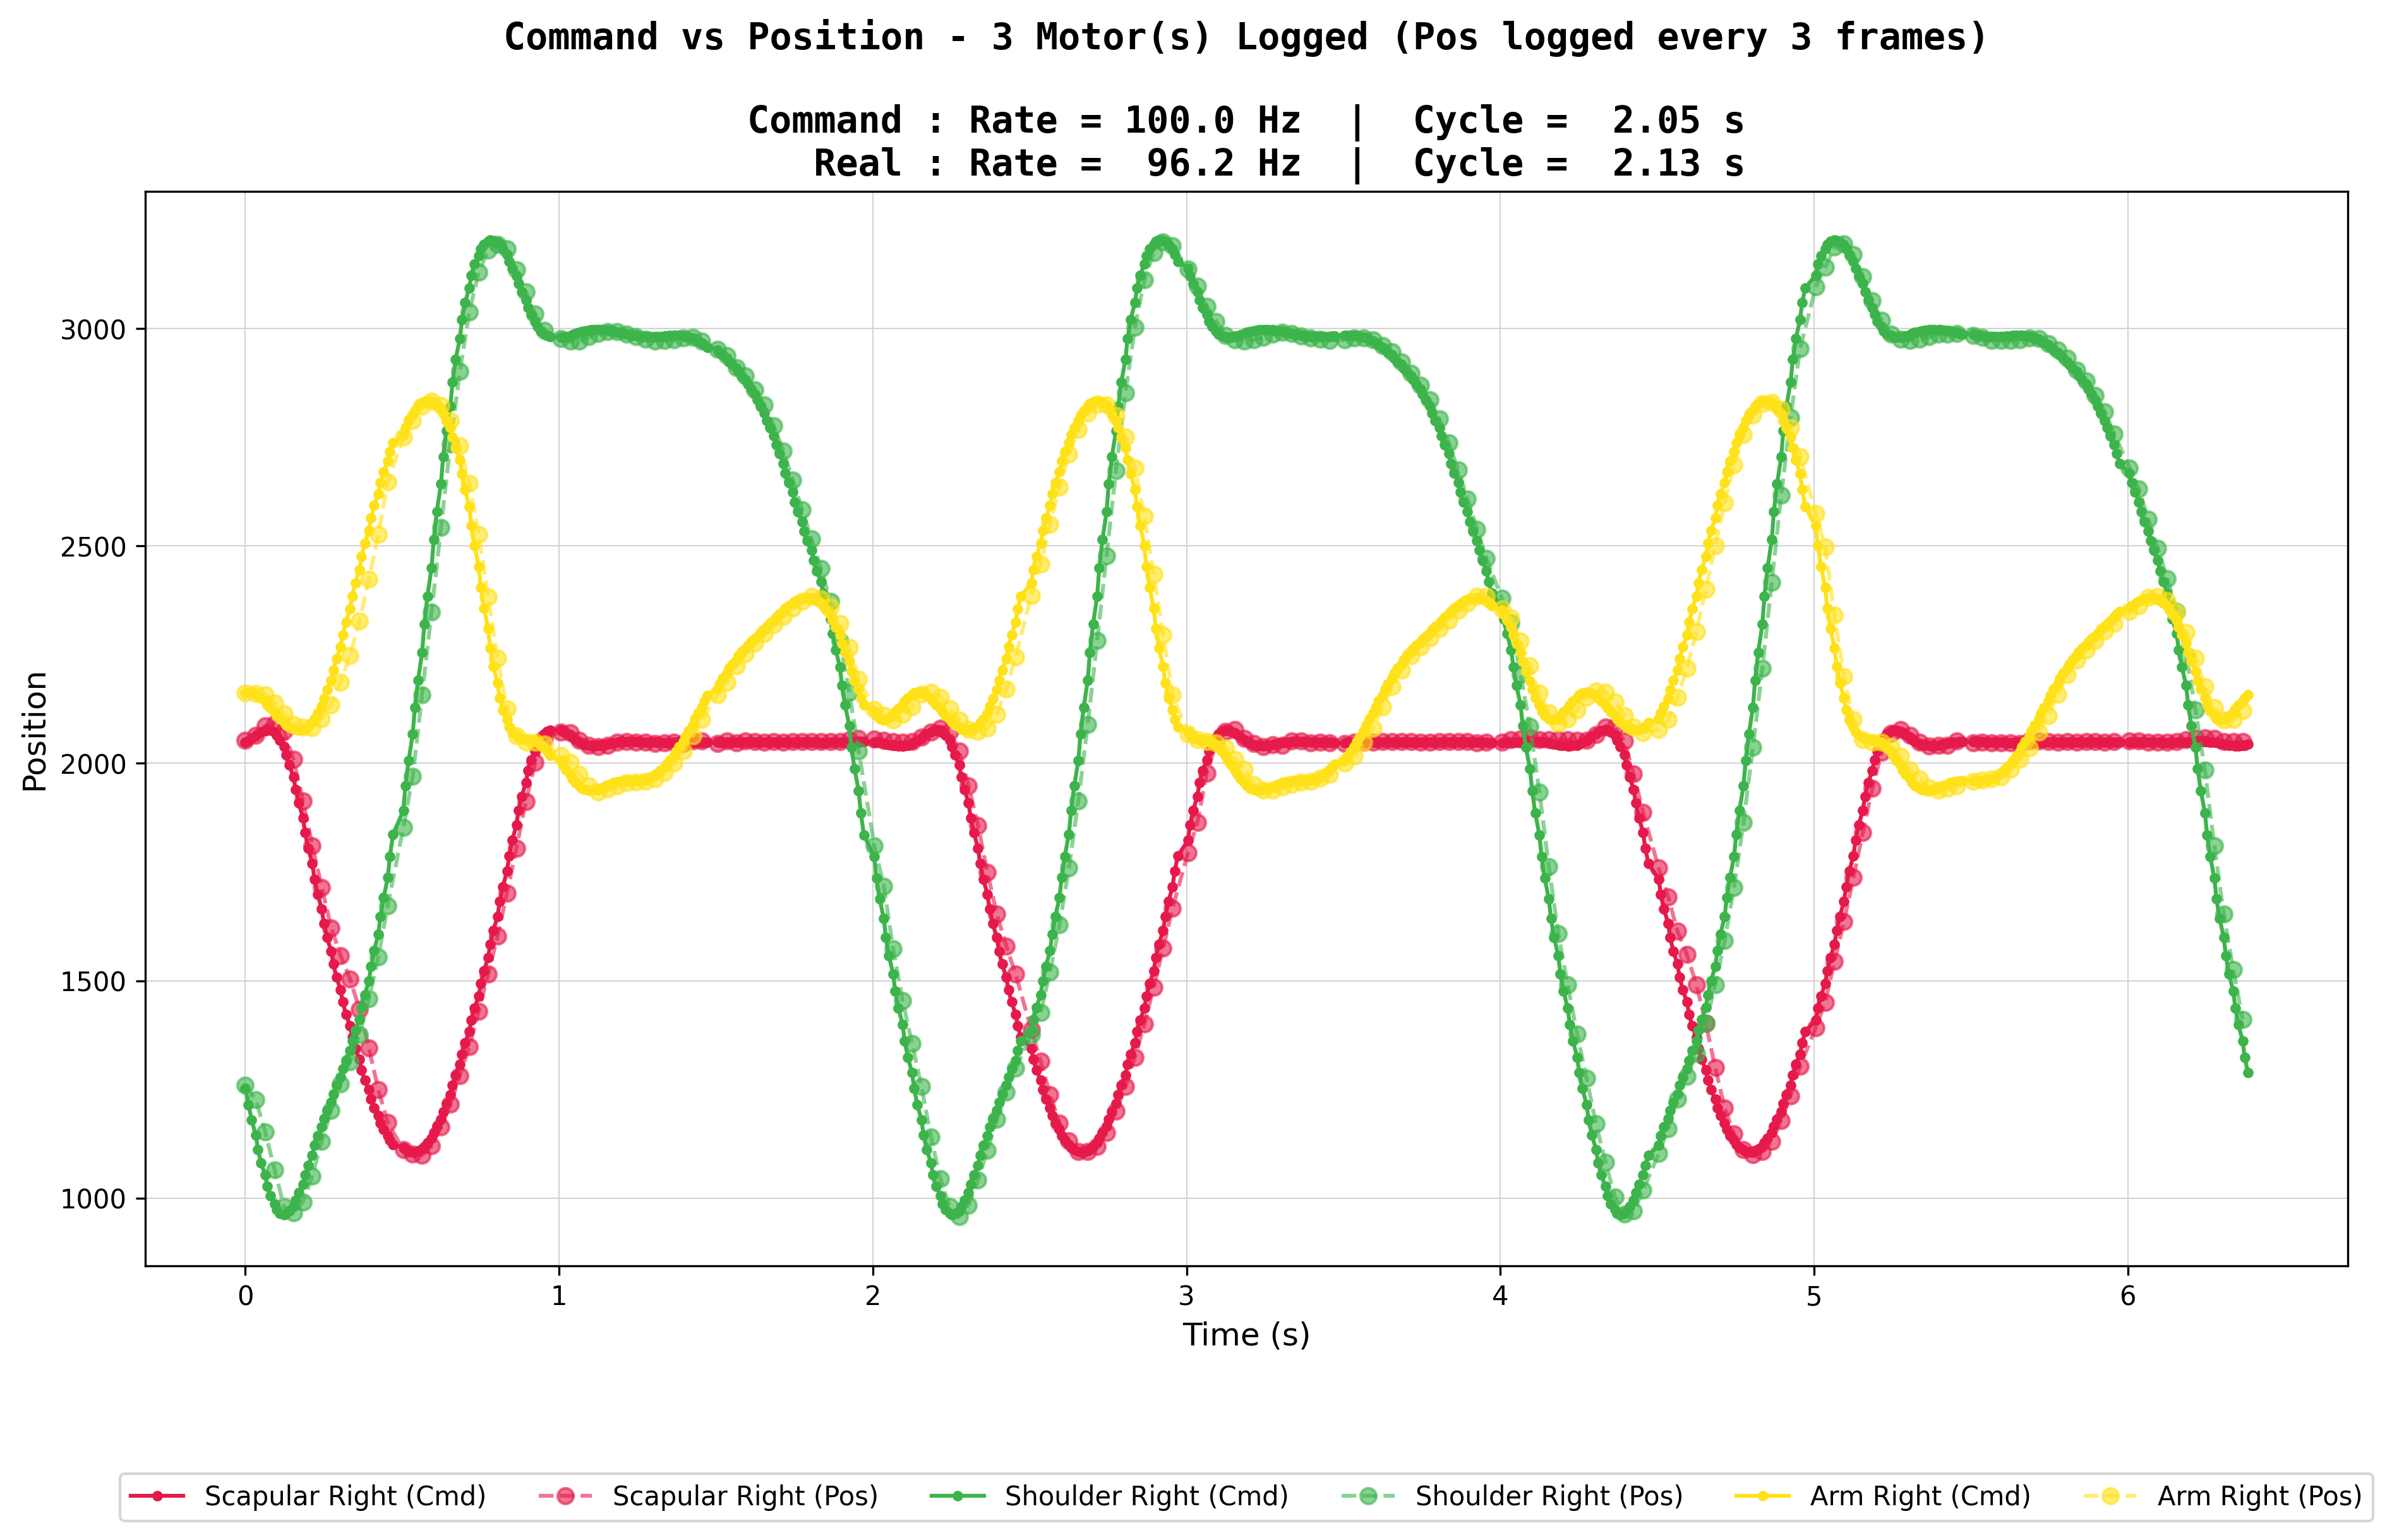
\includegraphics[width=\textwidth]{graphiques_swumanoid/swum_3mot_3f.png}
        \caption{3 motors $\rightarrow$ 96.2 Hz.}
    \end{subfigure}

    \vspace{0.35em}
    \begin{subfigure}[b]{0.48\textwidth}
        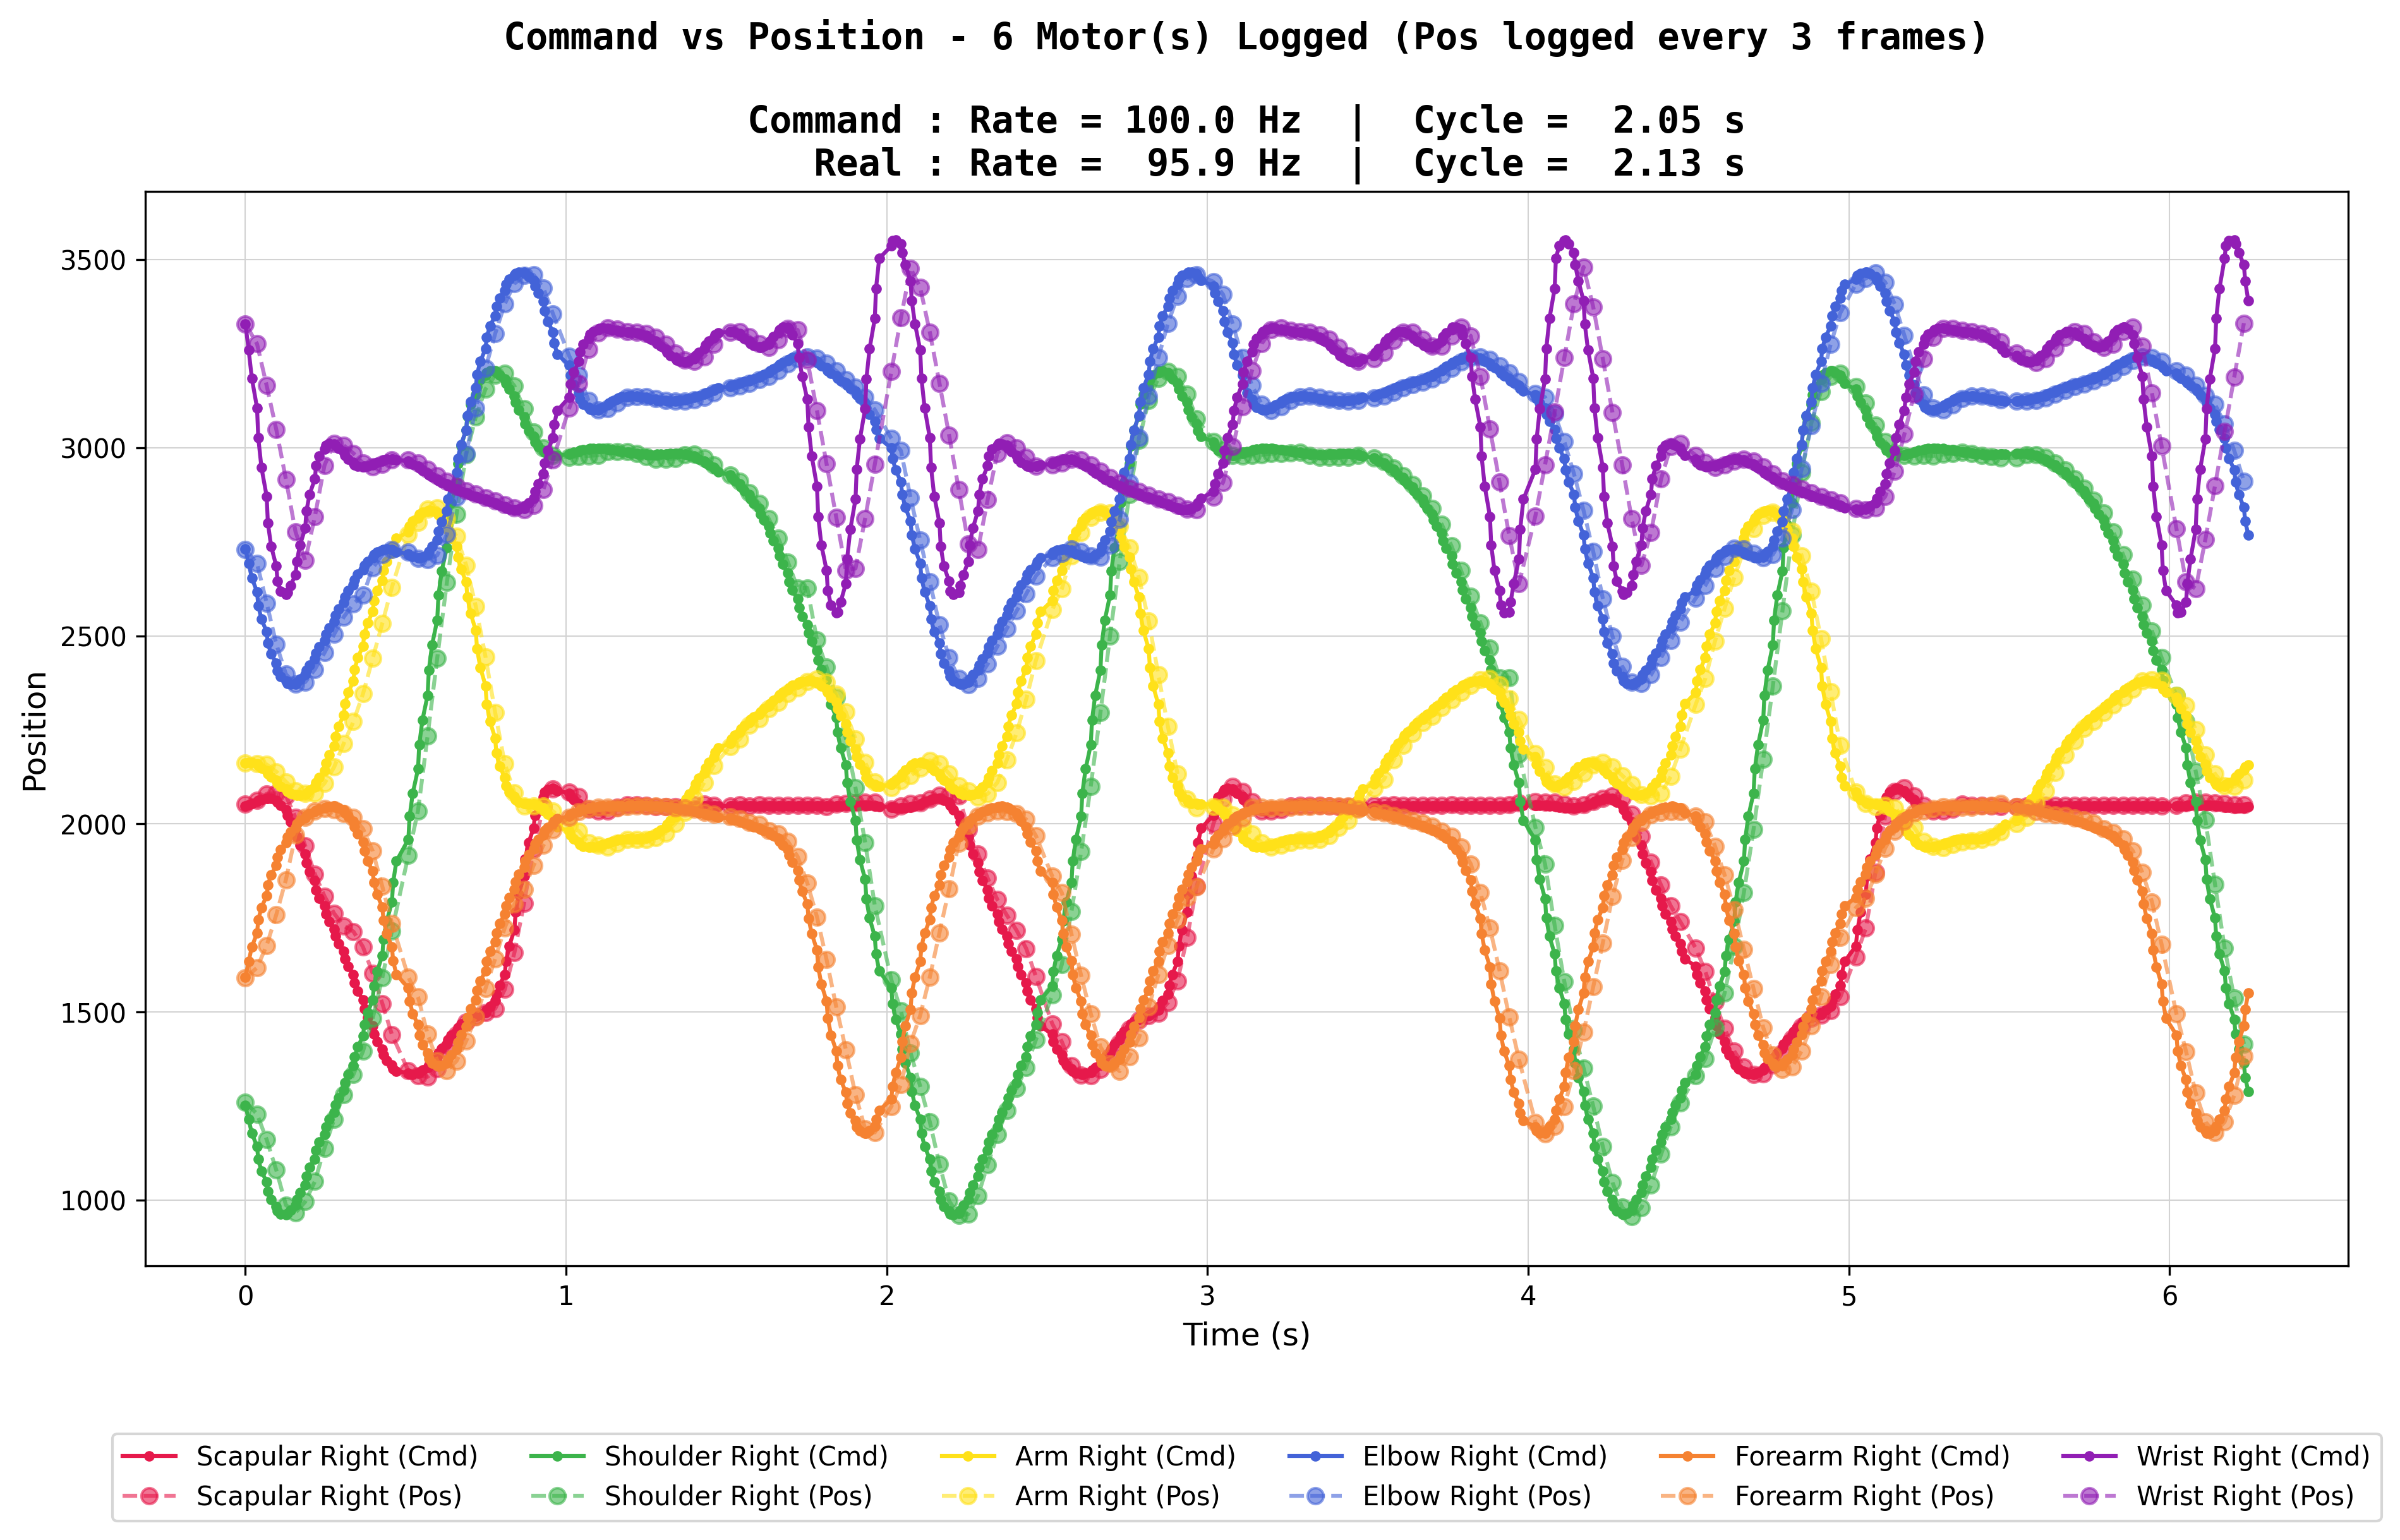
\includegraphics[width=\textwidth]{graphiques_swumanoid/swum_6mot_3f.png}
        \caption{6 motors $\rightarrow$ 95.9 Hz.}
    \end{subfigure}
    \hfill
    \begin{subfigure}[b]{0.48\textwidth}
        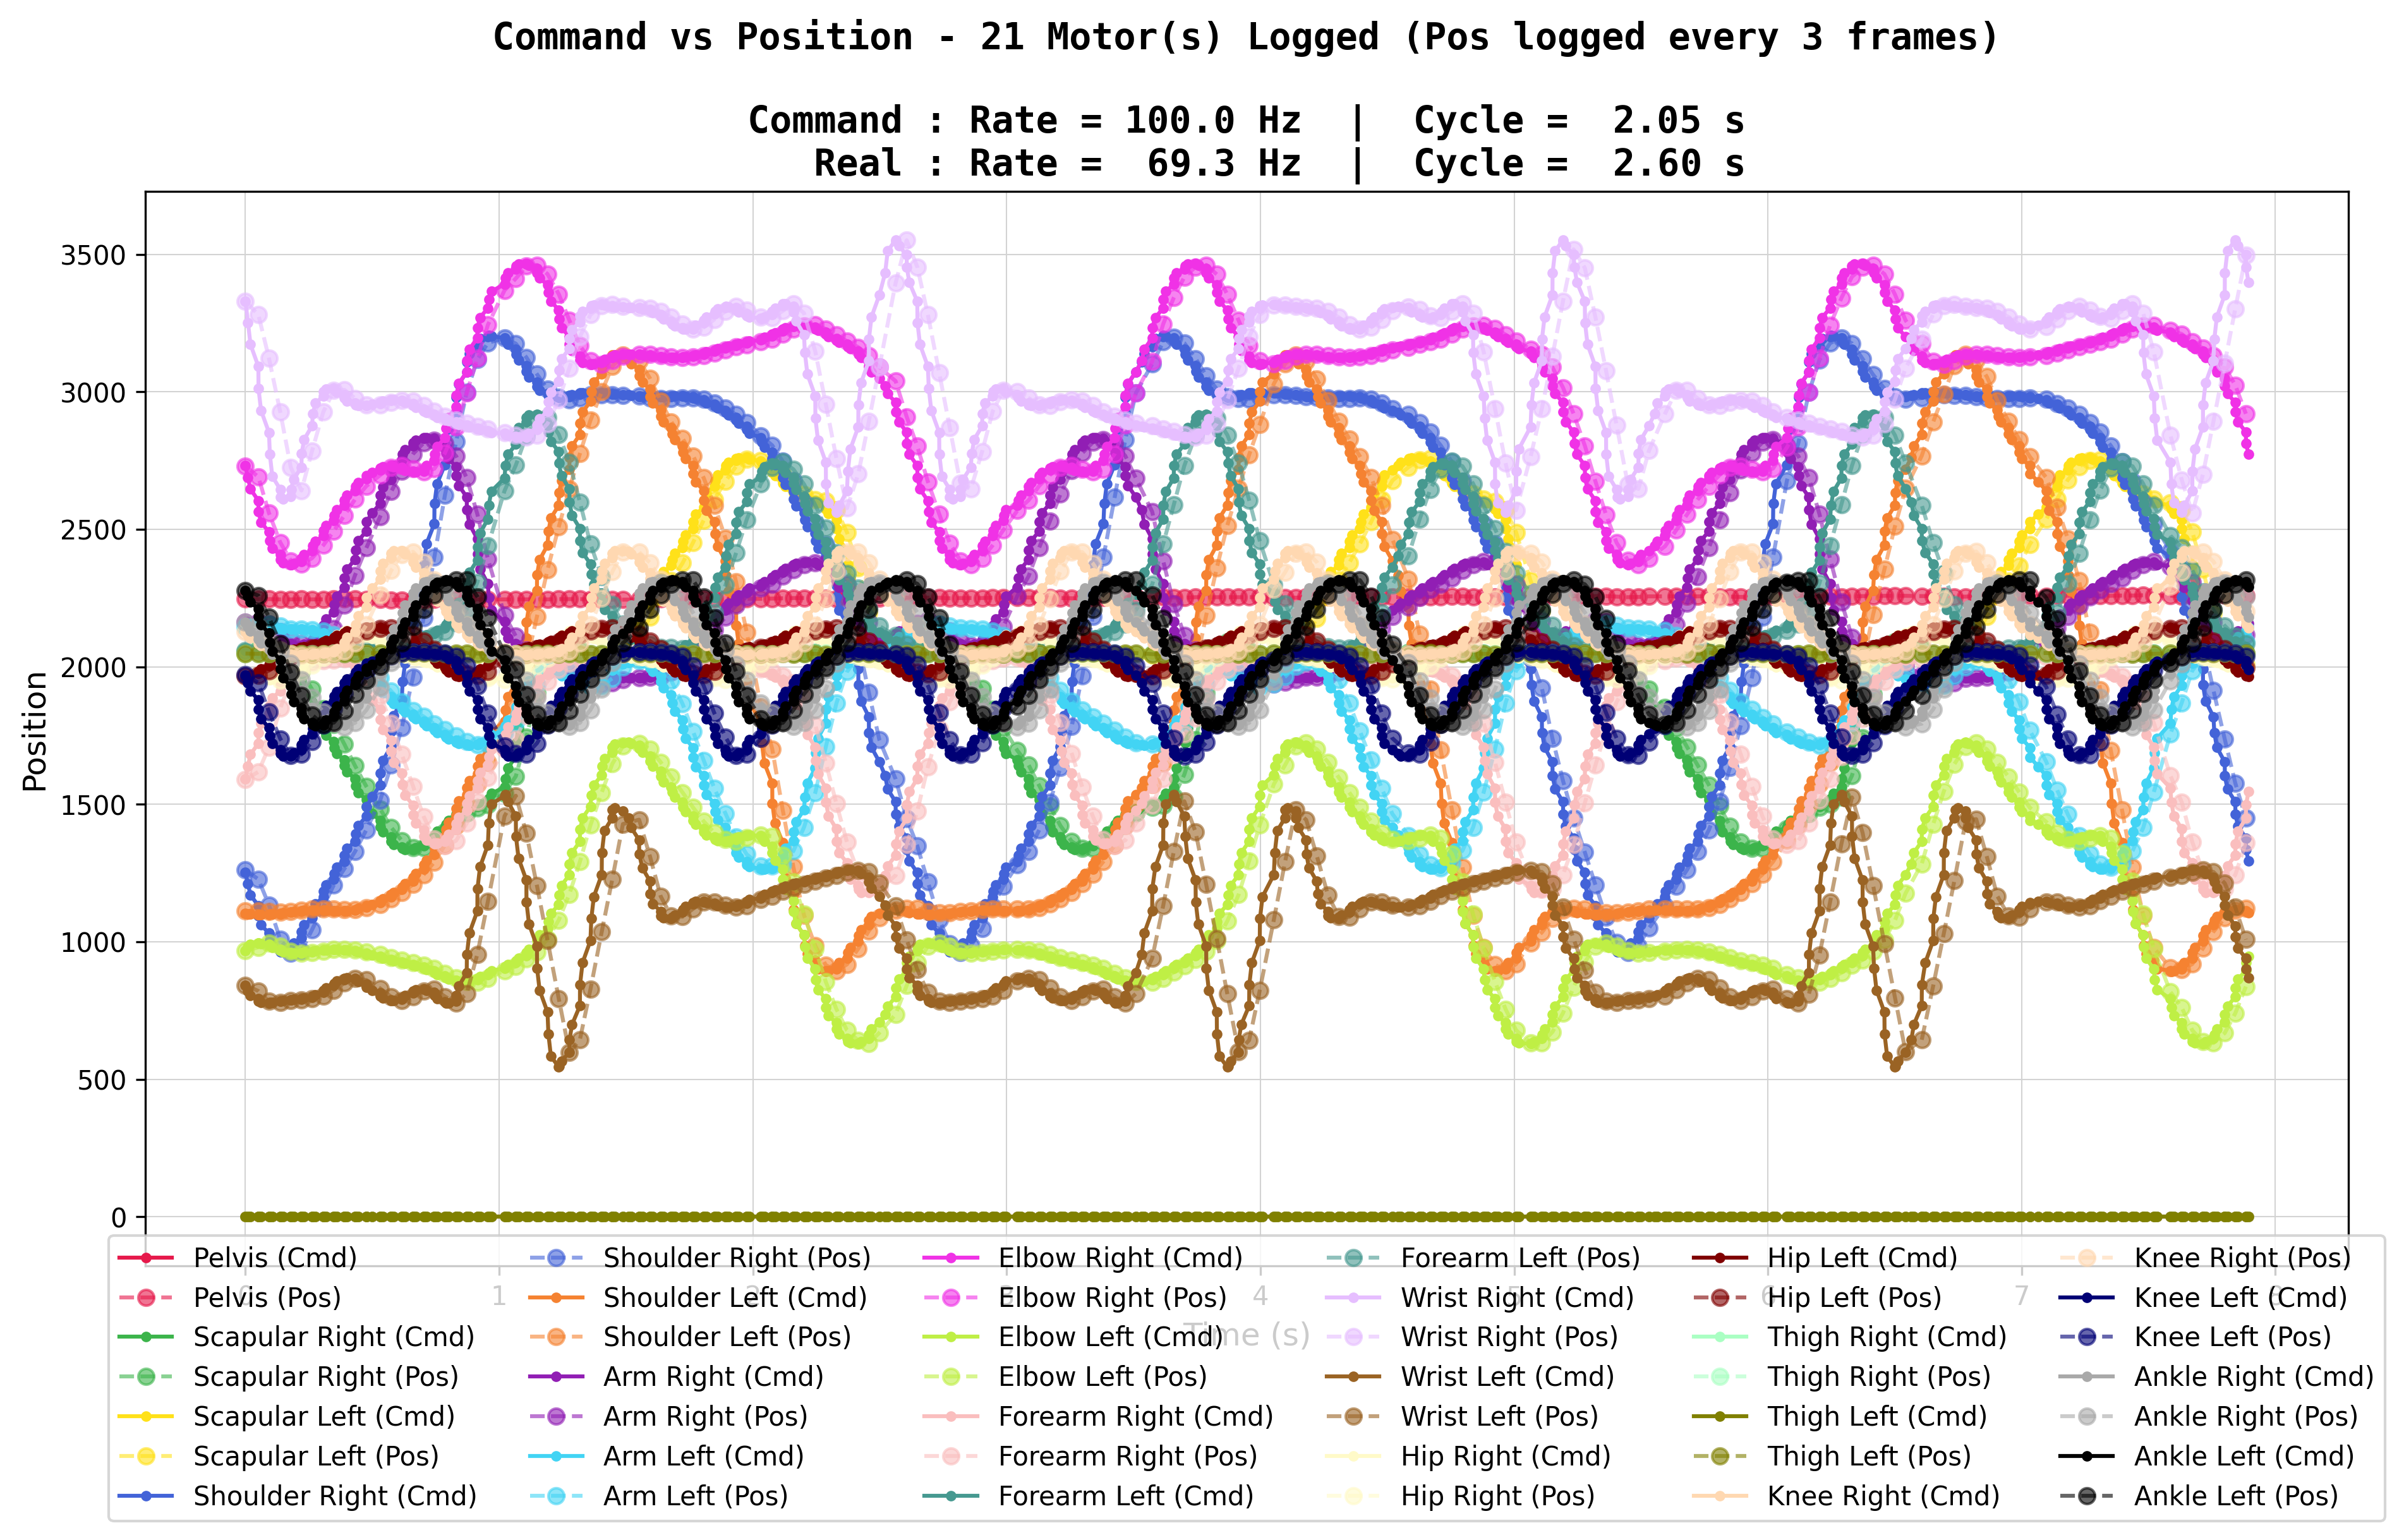
\includegraphics[width=\textwidth]{graphiques_swumanoid/swum_21mot_3f.png}
        \caption{21 motors $\rightarrow$ 69.3 Hz (real cycle 2.60\,s).}
        \label{fig:sswum_21_3f}
    \end{subfigure}
    \caption{Tests of the number of logged motors on the SWUMANOID, 100\,Hz, commanded cycle 2.05\,s, sampling every 3 frames.}
    \label{fig:swum_scaling}
\end{figure}
\fi

As we can see in the graph, up to six motors, logging is essentially \emph{free}, the real frequency stays capped at $\approx 96$\,Hz, that is, at the background deficit alone, independent of $N$, already identified. The read fits entirely within the 10\,ms margin. It was even possible to log all \textbf{21 motors} at once, the telemetry of the whole body in a single run, a really satisfying result. However, at that number and with such tight sampling (every 3 frames), reading the 21 sequential responses overflows the budget by a wide margin, in fact, the rate collapses to 69.3\,Hz and the real cycle time stretches to 2.60\,s, as shown in figure~\ref{fig:swum_21_3f}. Finally the whole body is recorded, but at the price of a loop far too slow.



While logging the entire body is possible, it makes the control loop too slow. The most logical solution, already anticipated by the model, is to \emph{reduce the frequency of the reads} rather than limit their content. So I raised the sampling interval from 3 to 6 frames, spacing out the \texttt{SyncRead} passes to give the bus more time between two queries. The result is presented in the figure~\ref{fig:swum_interval}:

\begin{figure}[H]
    \centering
    \begin{subfigure}[b]{0.48\textwidth}
        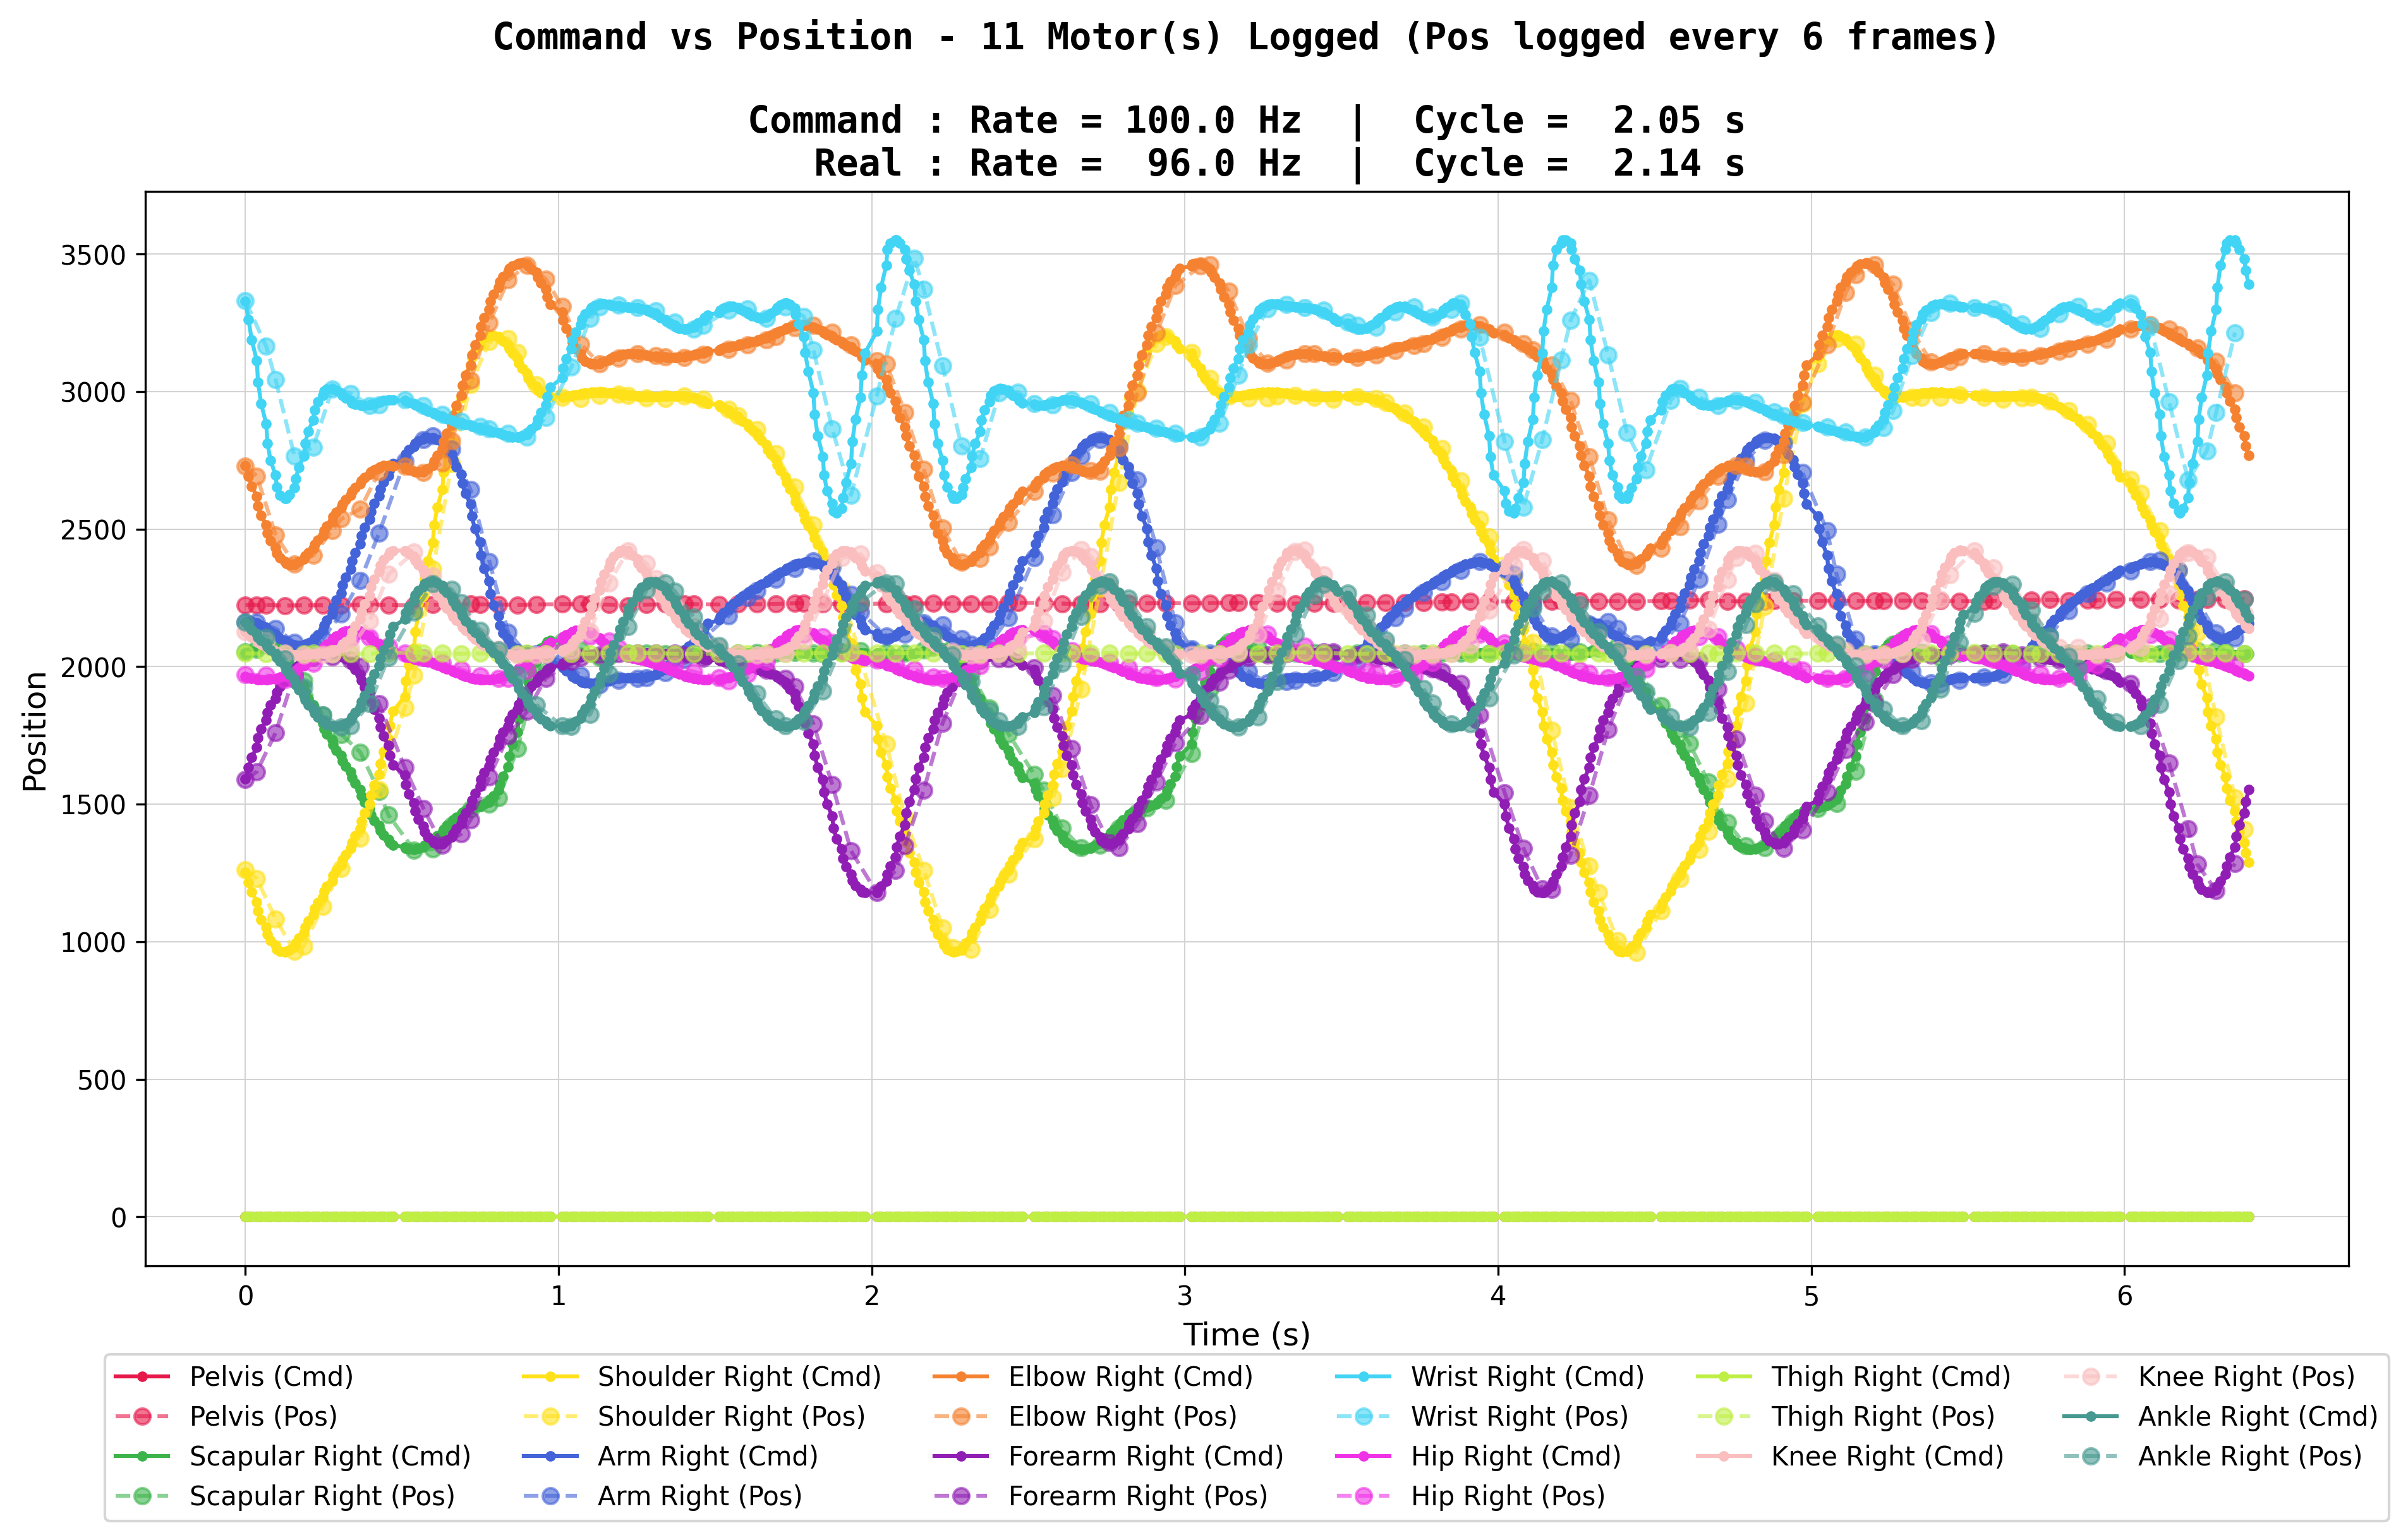
\includegraphics[width=\textwidth]{graphiques_swumanoid/swum_11mot_6f.png}
        \caption{11 motors, every 6 frames $\rightarrow$ 96.0 Hz.}
    \end{subfigure}
    \hfill
    \begin{subfigure}[b]{0.48\textwidth}
        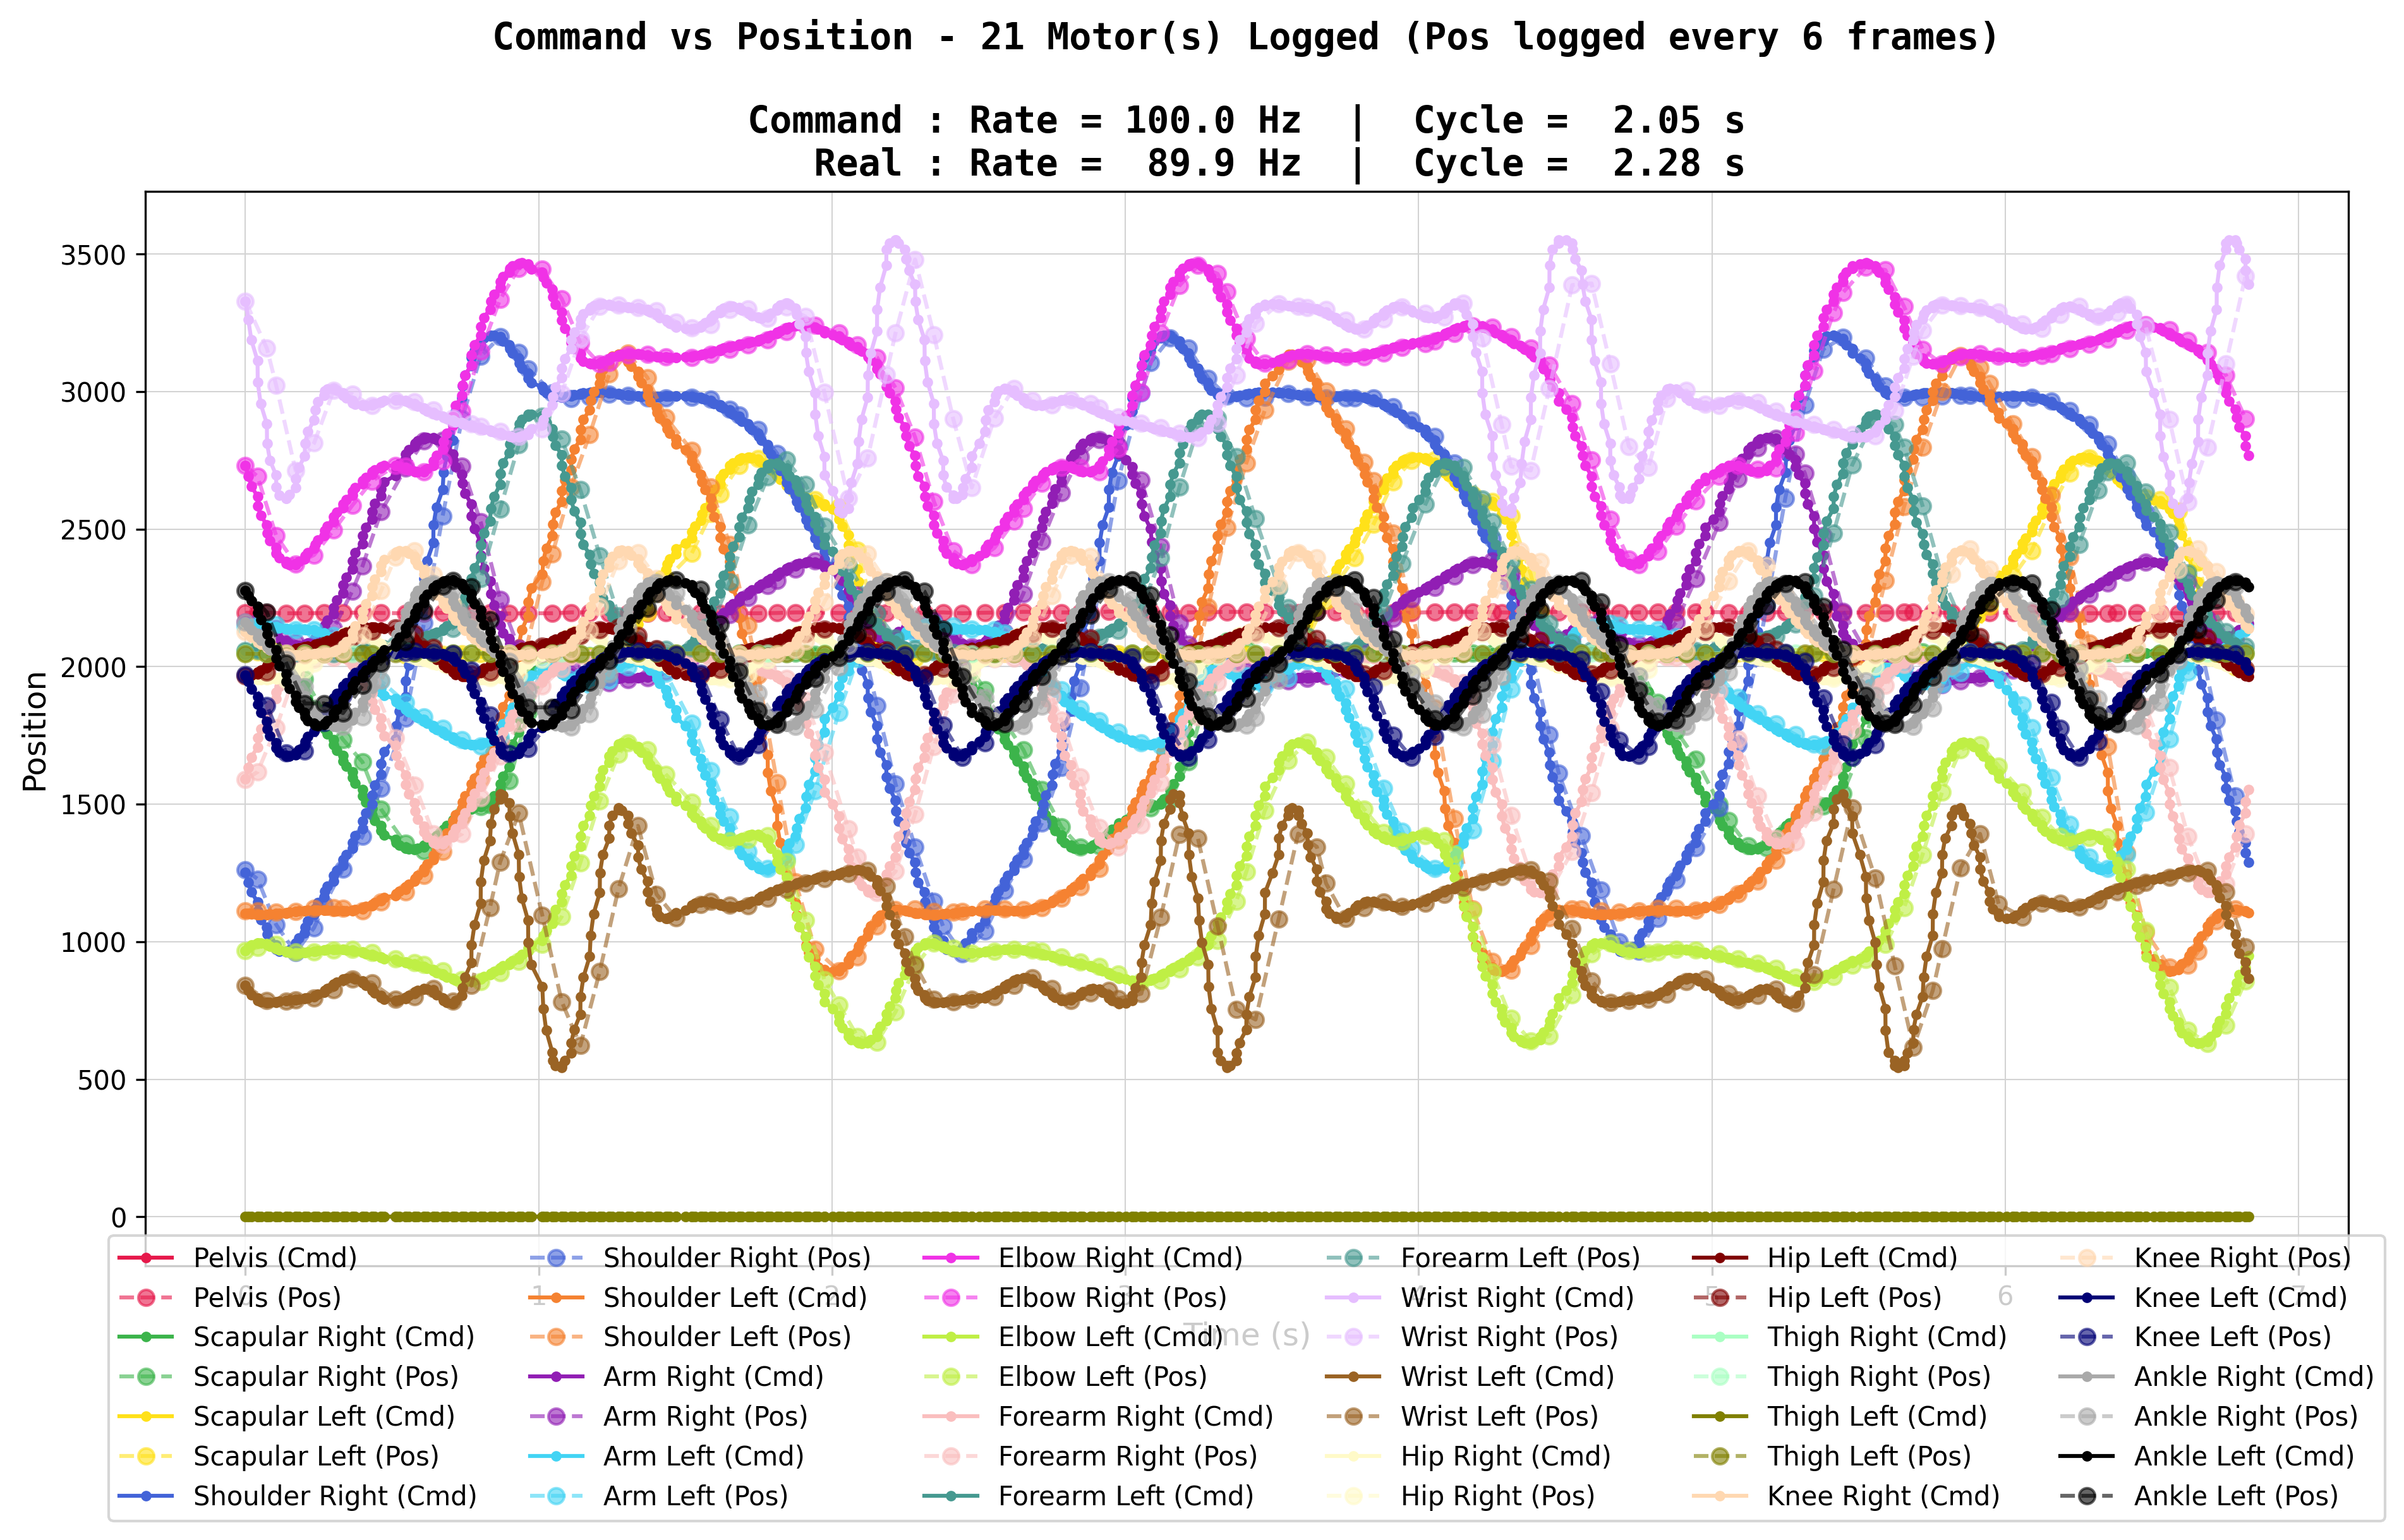
\includegraphics[width=\textwidth]{graphiques_swumanoid/swum_21mot_6f.png}
        \caption{21 motors, every 6 frames $\rightarrow$ 89.9 Hz.}
    \end{subfigure}
    \caption{Effect of the sampling interval (100\,Hz, commanded cycle 2.05\,s).}
    \label{fig:swum_interval}
\end{figure}

At 21 motors, the rate climbs from 69.3\,Hz back up to \textbf{89.9\,Hz}, and at 11 motors it even returns to the background ceiling ($\approx 96$\,Hz). Quantitatively, the amortized read overhead per frame drops from $\approx 4.4$\,ms (at 3 frames) to $\approx 1.1$\,ms (at 6 frames), this reduction beats the factor of two expected from simply doubling the interval, since the wider spacing also gives the bus a recovery time that lightens the cost of each read. Doubling the sampling interval thus restores most of the rate while keeping full coverage of the 21 motors.

With 21 motors logged every 6 frames, the $\approx 90$\,Hz rate is satisfying, but the real cycle time stays above the setpoint (2.28\,s for a commanded 2.05\,s). Indeed, the trajectory holds a fixed number of frames ($\text{cycle} \times \text{rate}$), and replaying them at 90\,Hz instead of 100\,Hz mechanically stretches the duration by a factor of $100/90 \approx 1.11$. So, as a last step, I varied only the commanded cycle time, with every other parameter frozen presentend in the figure~\ref{fig:swum_cycle} and the table~\ref{tab:swum_cycle} below :

\iffalse
\begin{figure}[H]
    \centering
    \begin{subfigure}[b]{0.48\textwidth}
        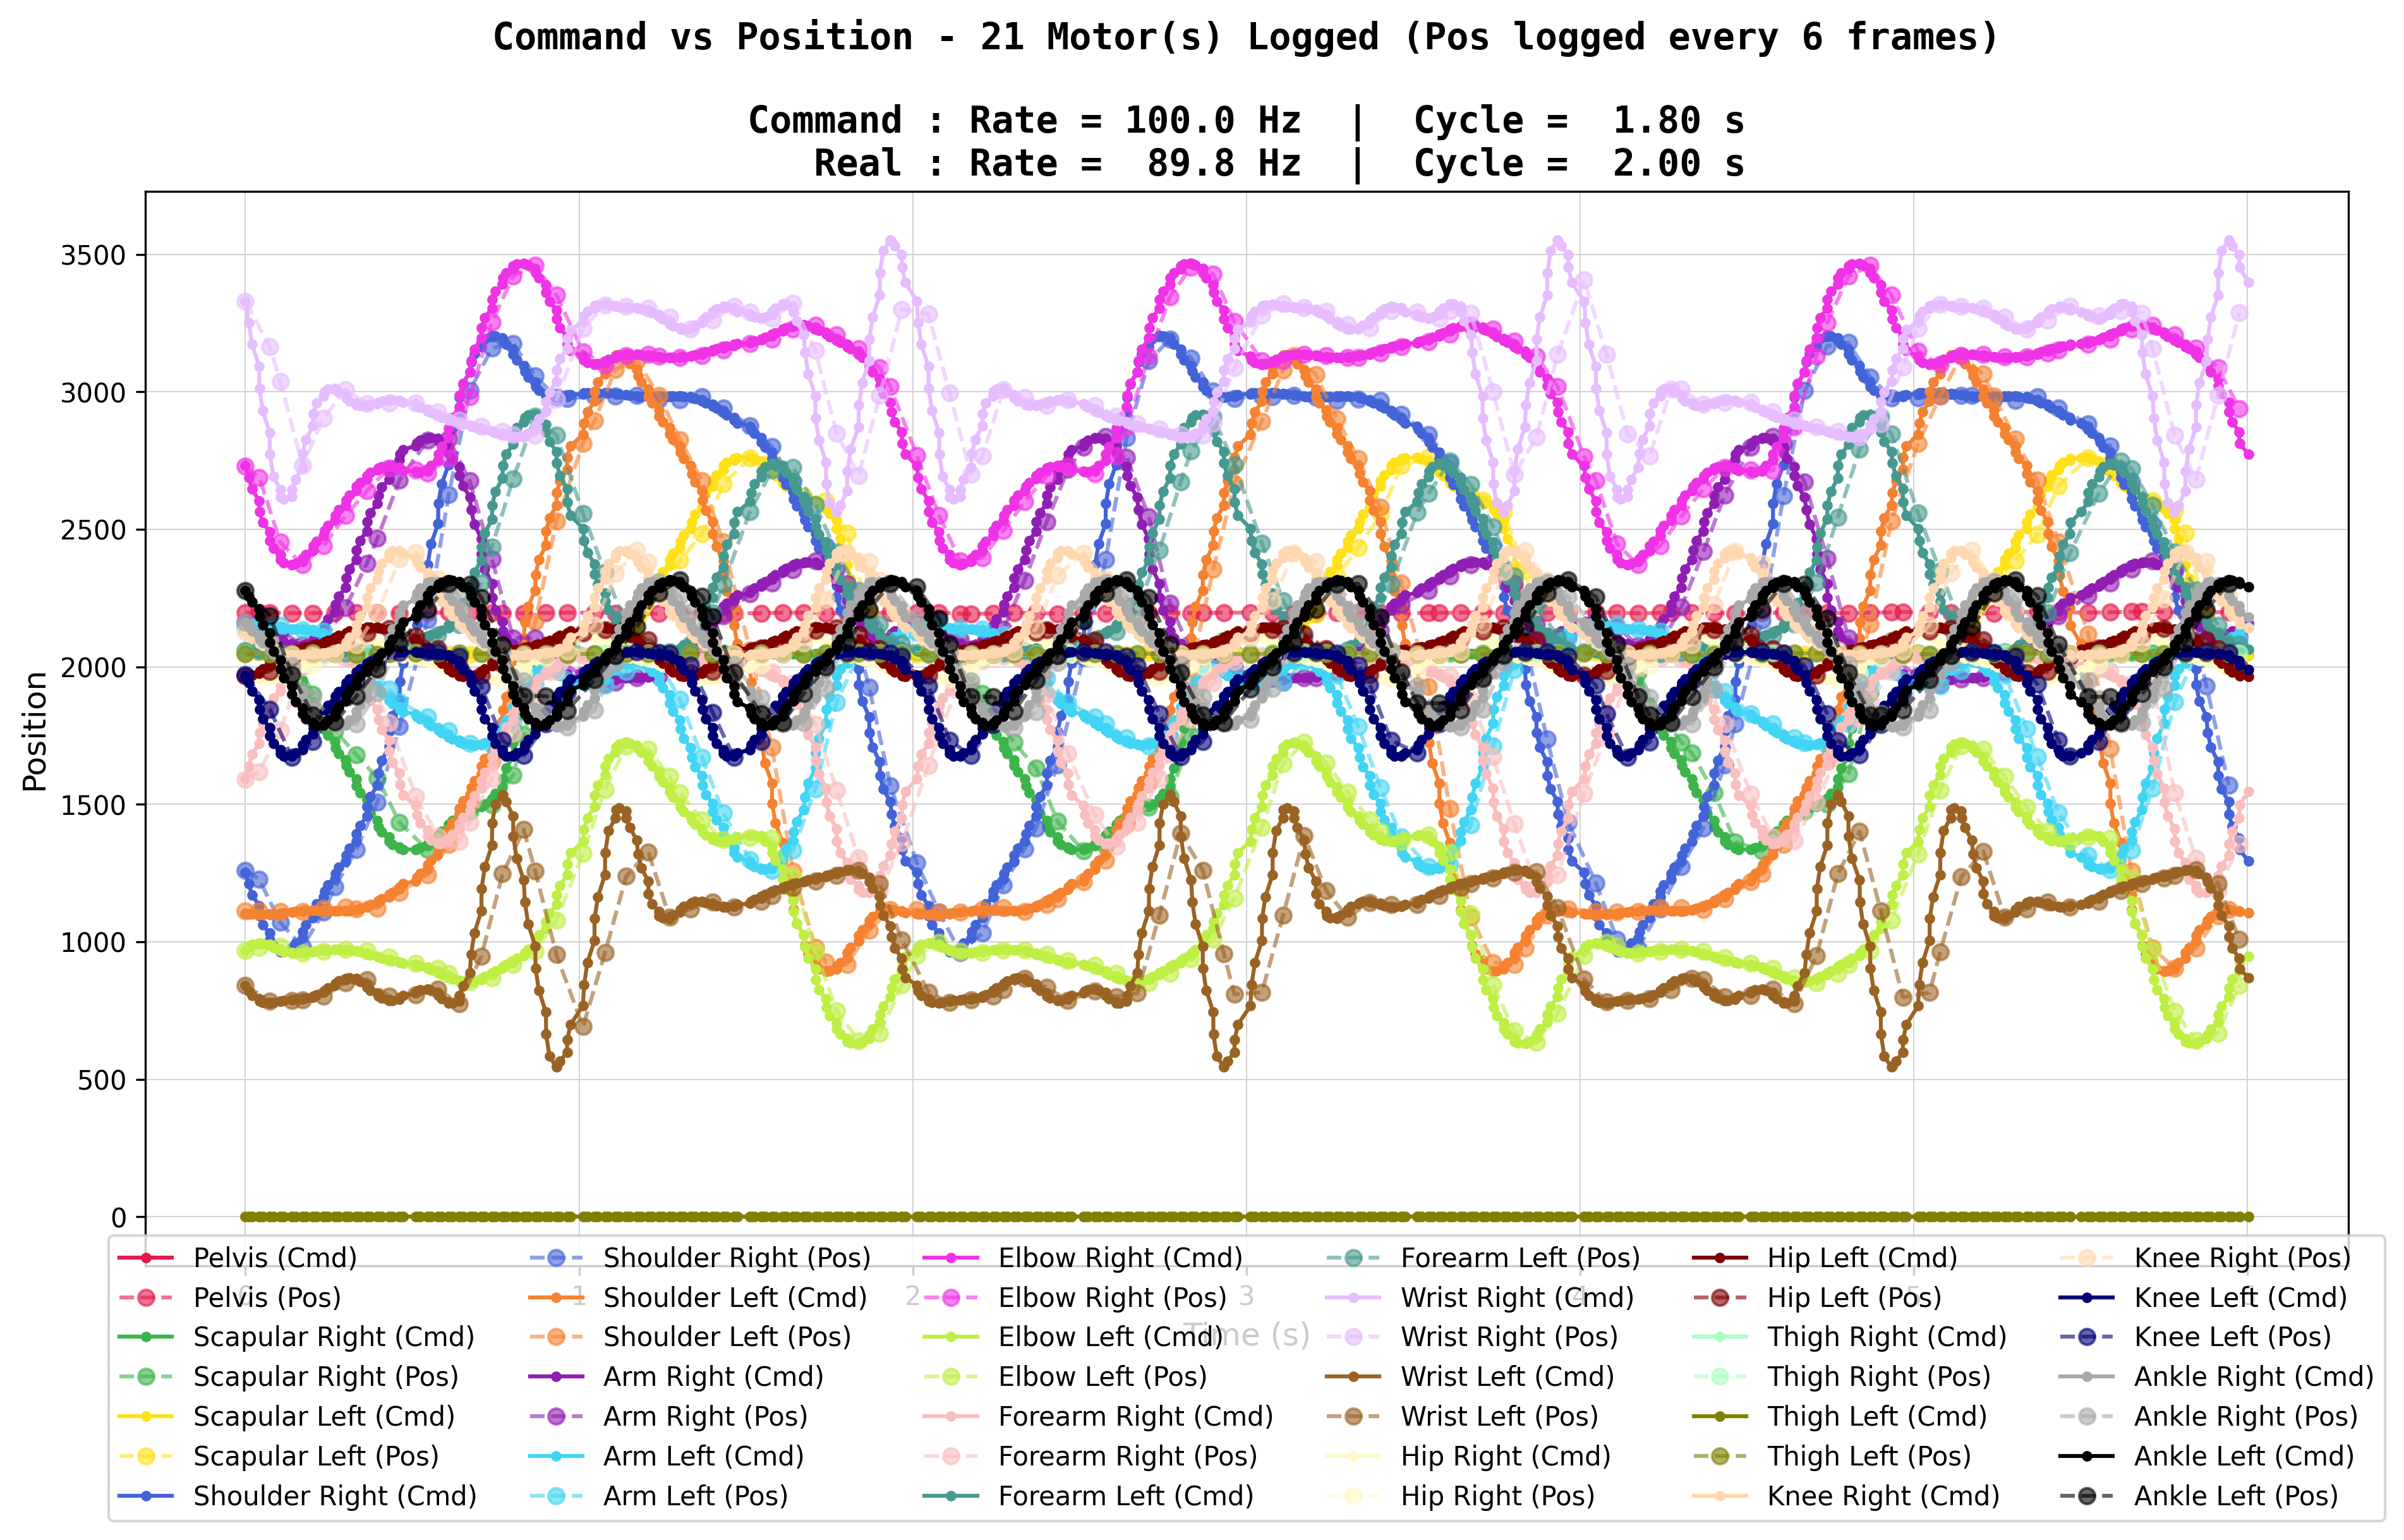
\includegraphics[width=\textwidth]{graphiques_swumanoid/swum_21mot_6f_cmd1p80.png}
        \caption{Commanded cycle 1.80\,s $\rightarrow$ real cycle \textbf{2.00\,s} (89.8 Hz).}
        \label{fig:sswum_best}
    \end{subfigure}
    \hfill
    \begin{subfigure}[b]{0.48\textwidth}
        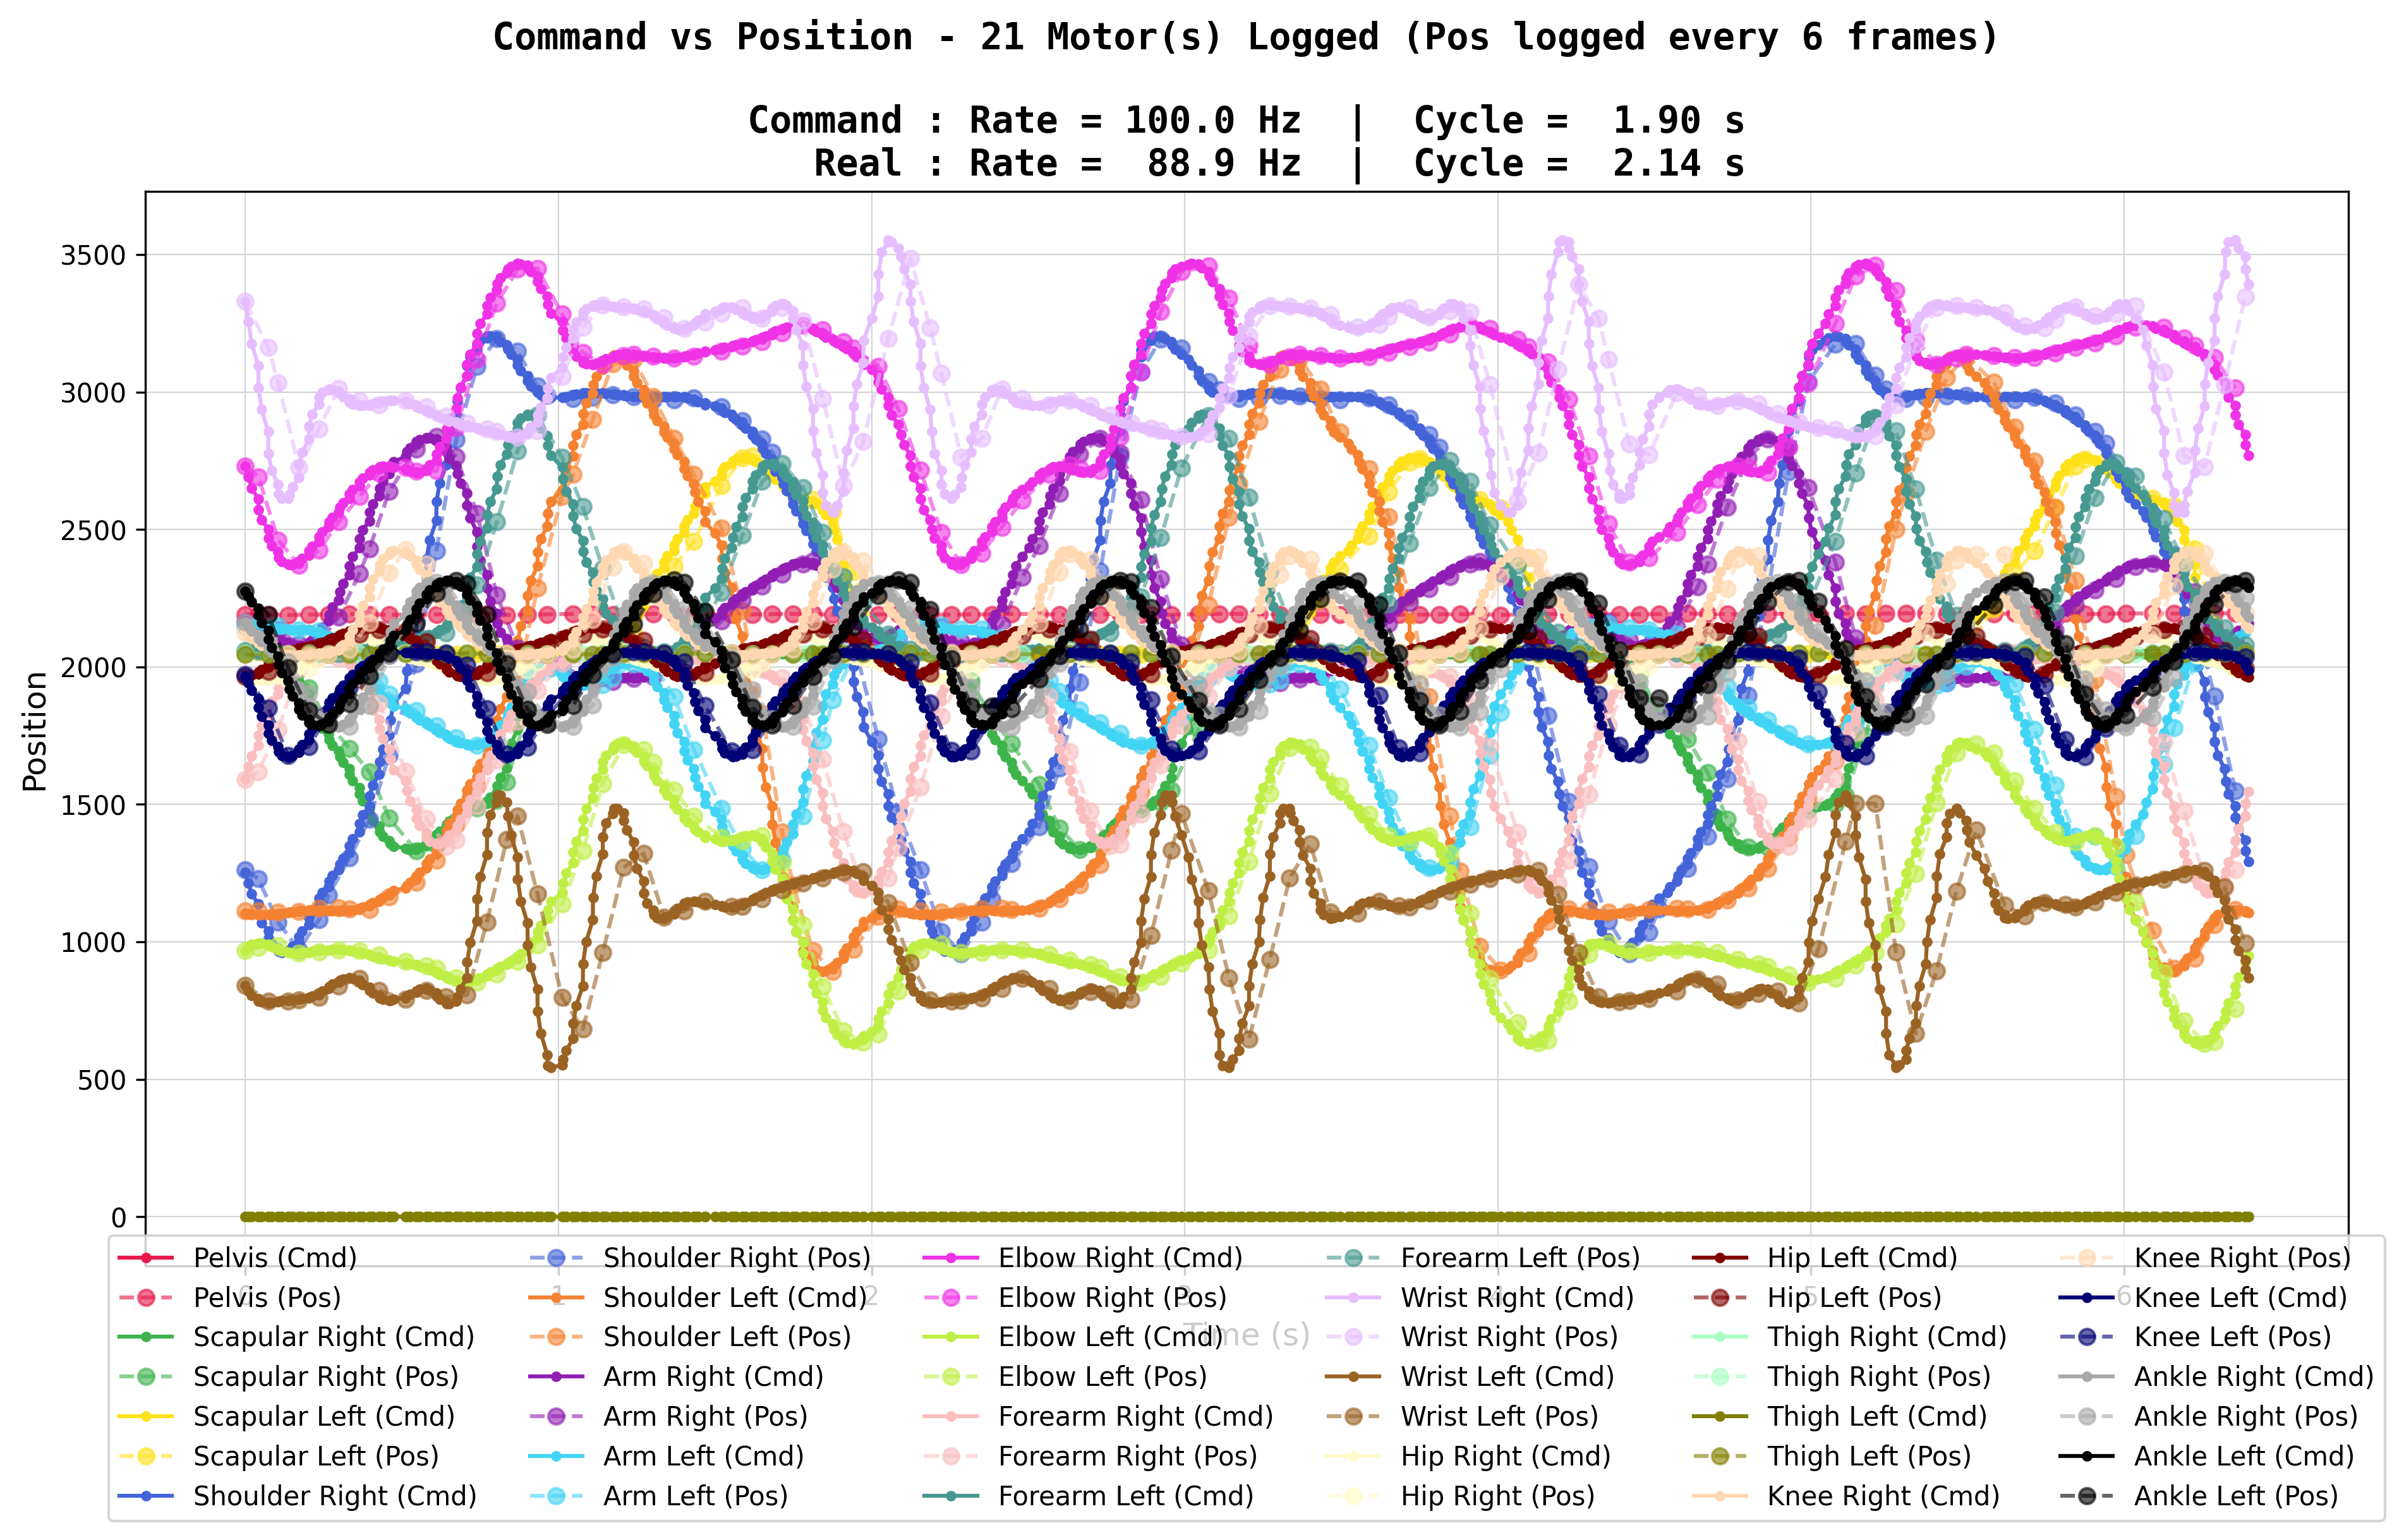
\includegraphics[width=\textwidth]{graphiques_swumanoid/swum_21mot_6f_cmd1p90.png}
        \caption{Commanded cycle 1.90\,s $\rightarrow$ real cycle 2.14\,s (88.9 Hz).}
    \end{subfigure}
    \caption{Sweep of the commanded cycle time (1.80\,s and 1.90\,s), 100\,Hz, 21 motors, sampling every 6 frames.}
    \label{fig:swum_cycle_part1}
\end{figure}

\begin{figure}[H]
    \centering
    \begin{subfigure}[b]{0.48\textwidth}
        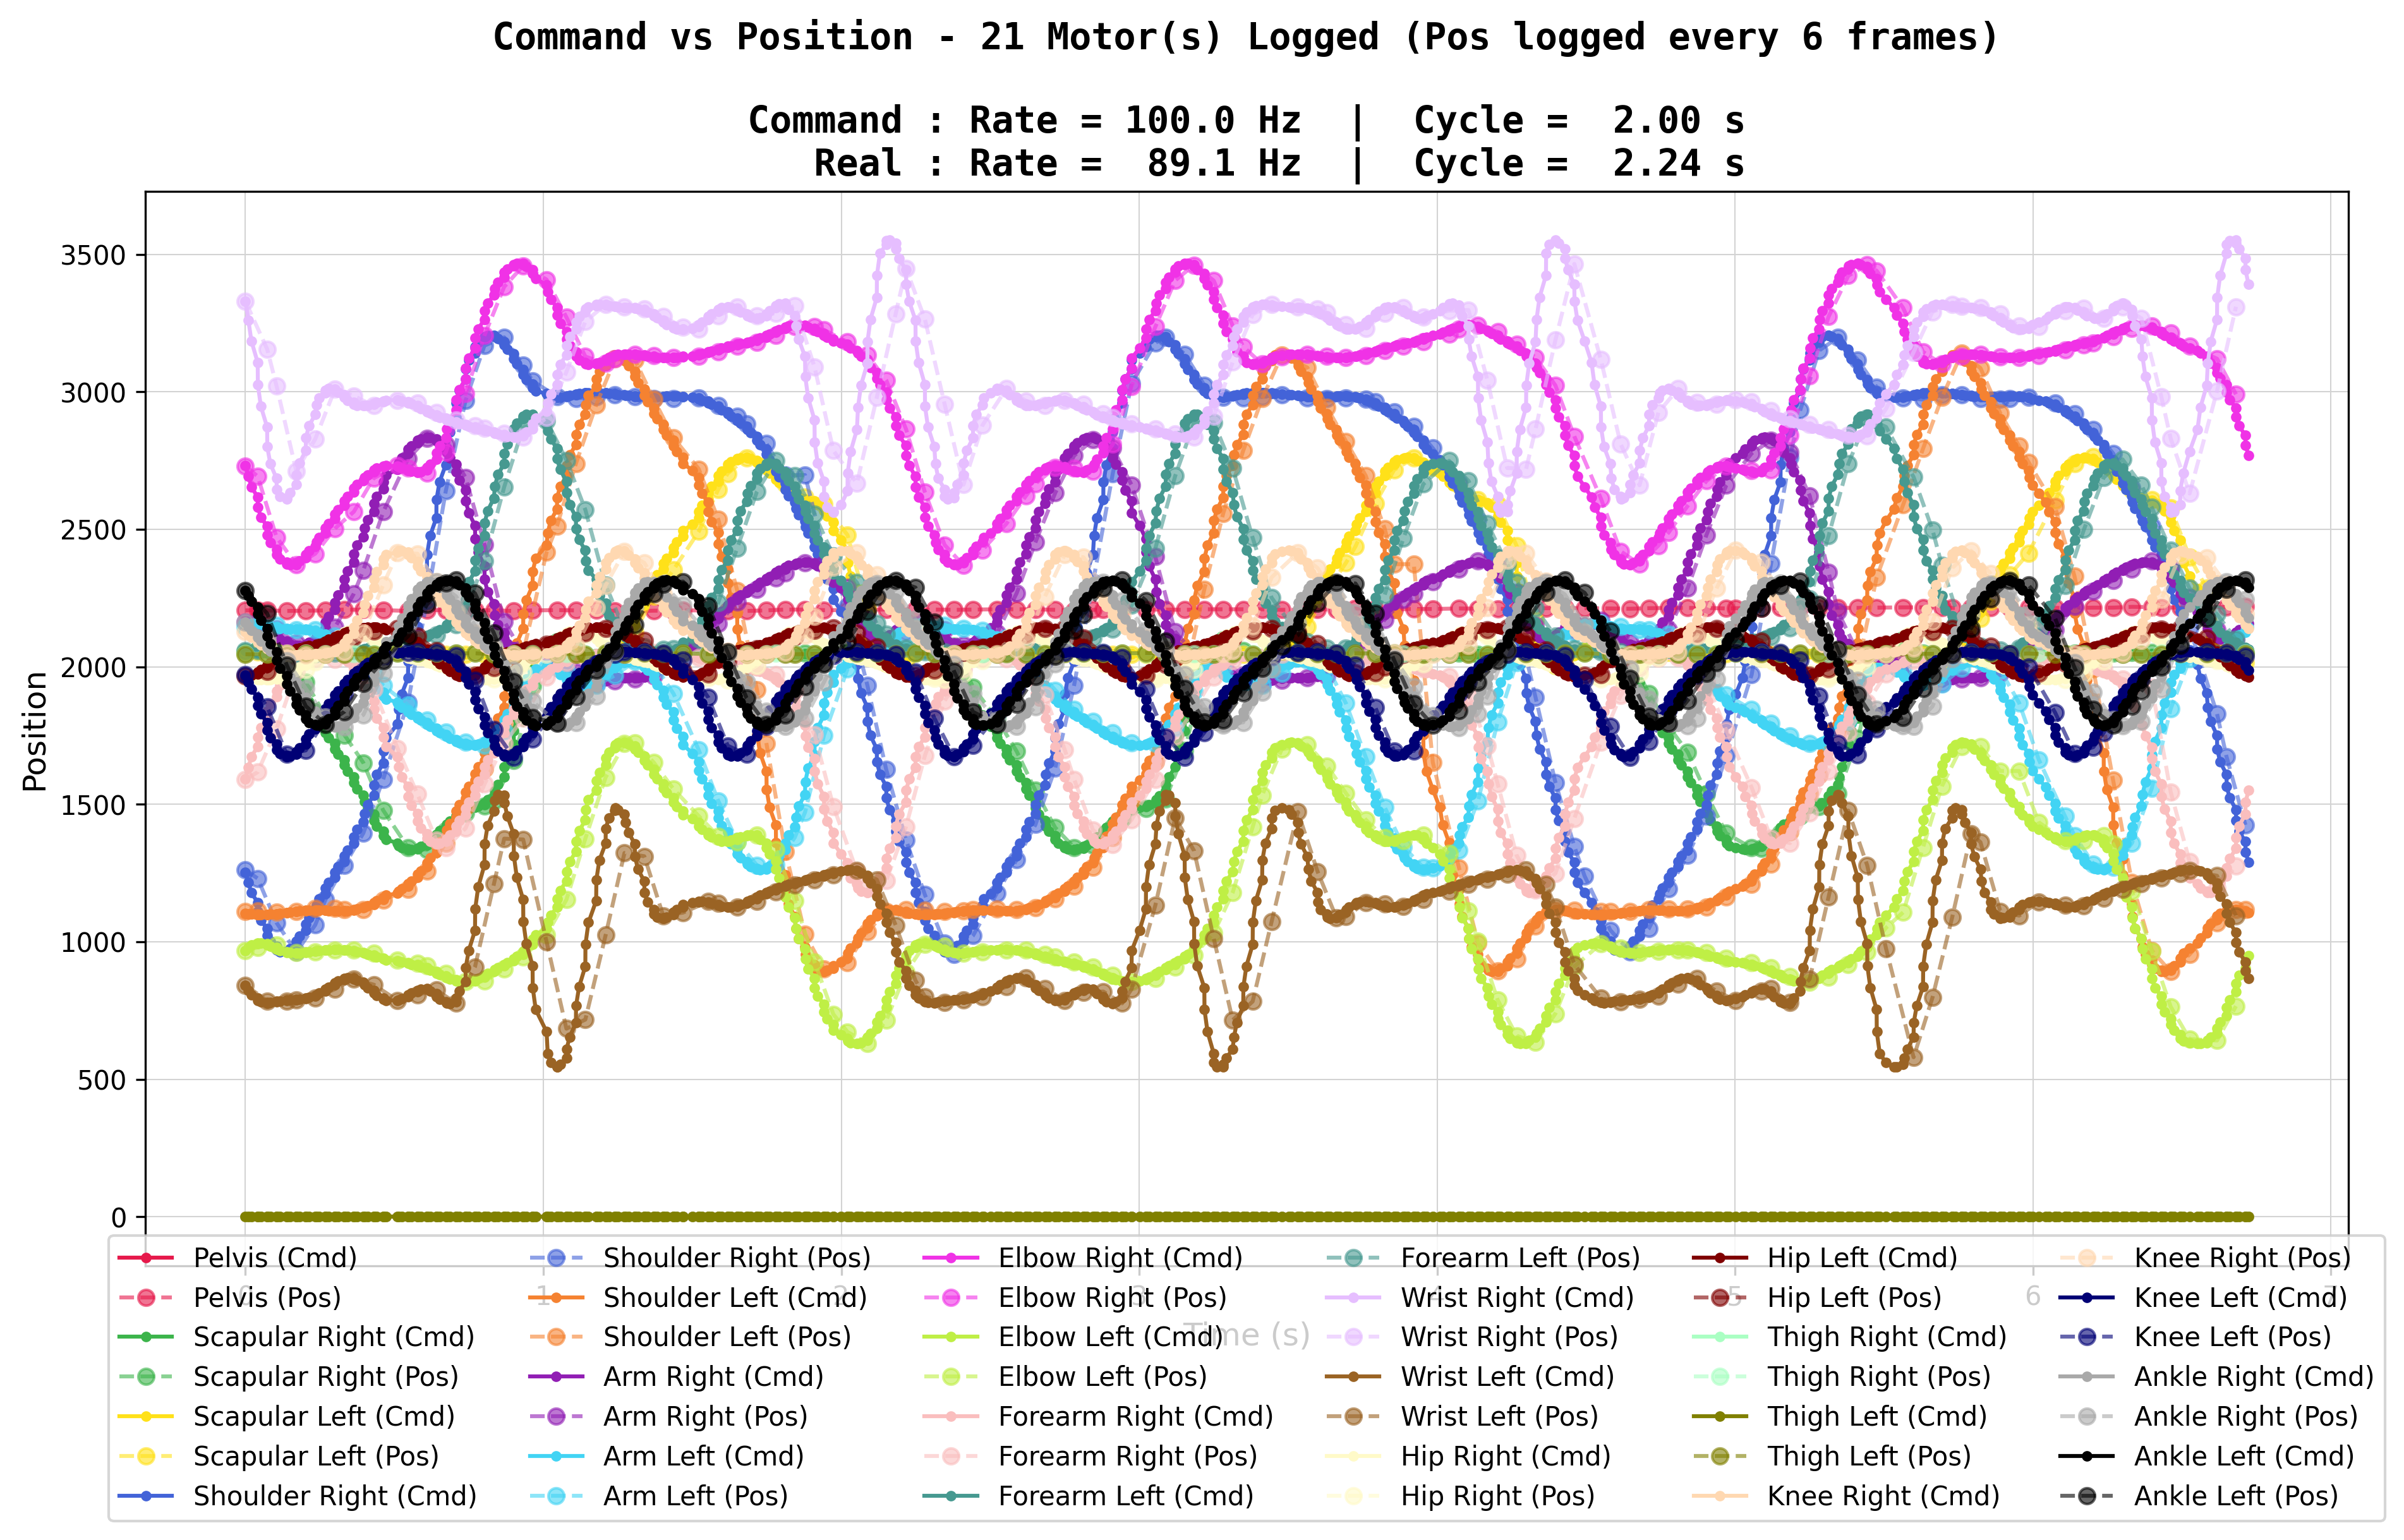
\includegraphics[width=\textwidth]{graphiques_swumanoid/swum_21mot_6f_cmd2p00.png}
        \caption{Commanded cycle 2.00\,s $\rightarrow$ real cycle 2.24\,s (89.1 Hz).}
    \end{subfigure}
    \hfill
    \begin{subfigure}[b]{0.48\textwidth}
        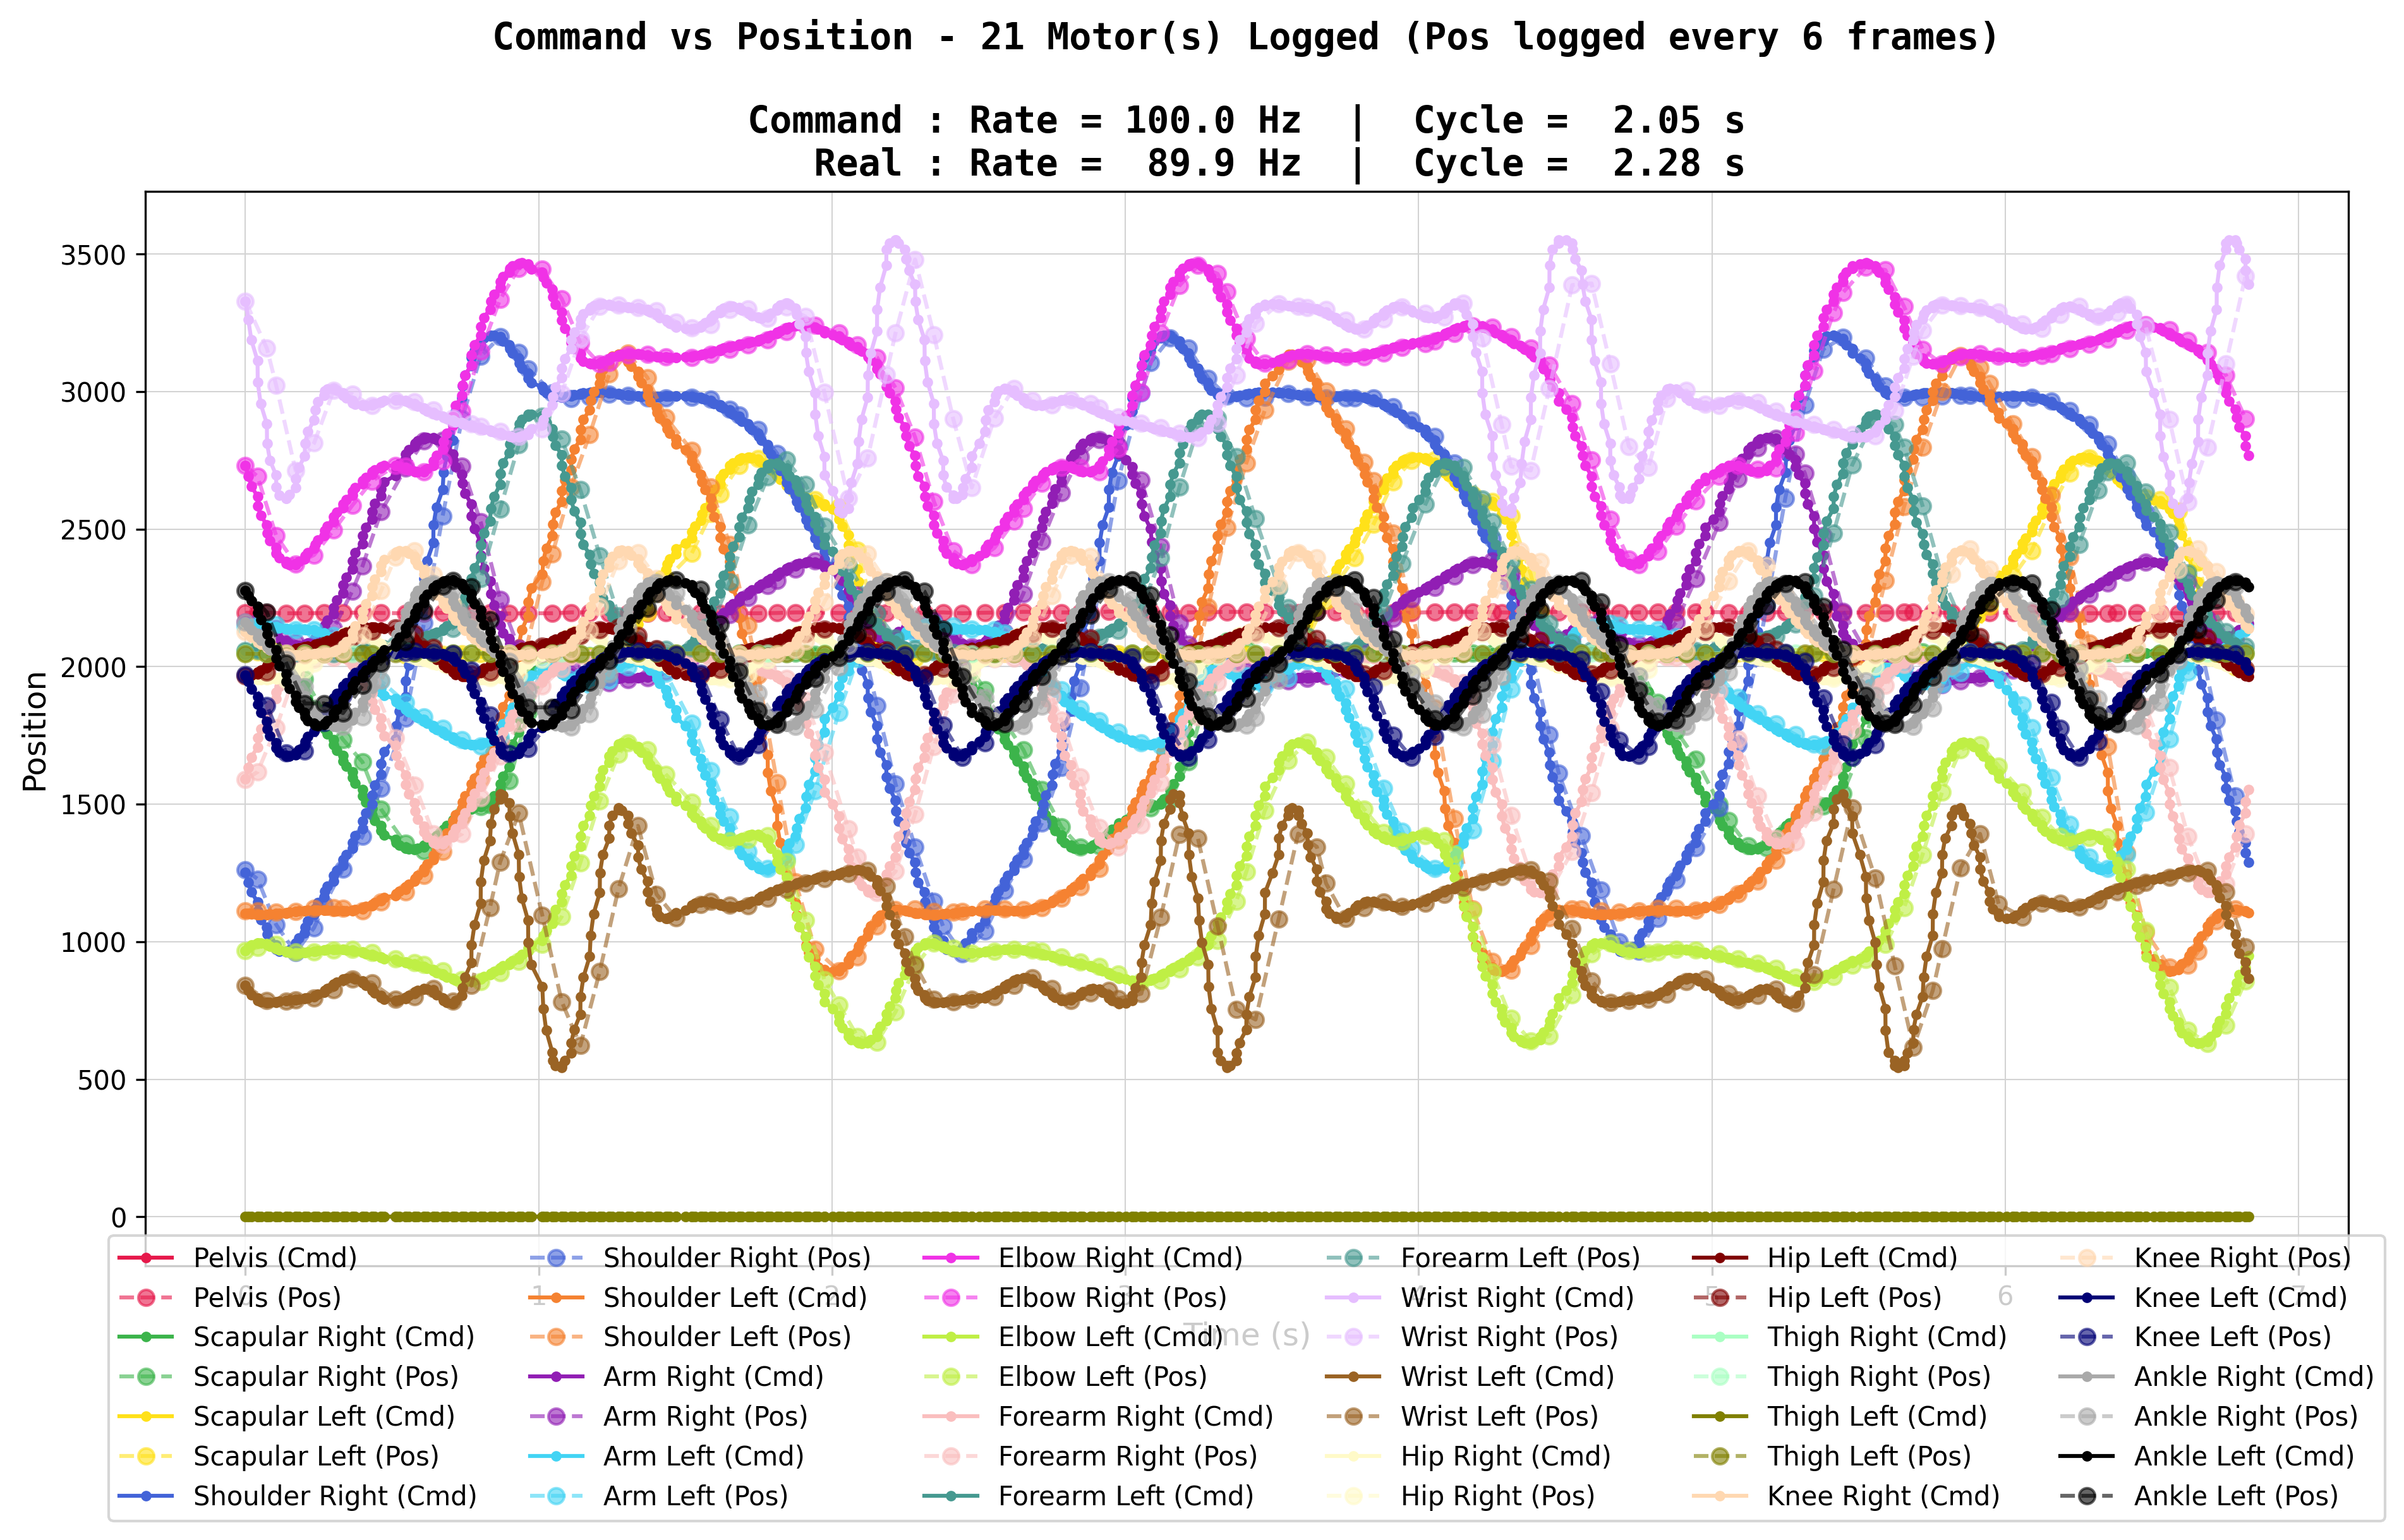
\includegraphics[width=\textwidth]{graphiques_swumanoid/swum_21mot_6f.png}
        \caption{Commanded cycle 2.05\,s $\rightarrow$ real cycle 2.28\,s (89.9 Hz).}
    \end{subfigure}
    \caption{Sweep of the commanded cycle time (2.00\,s and 2.05\,s), 100\,Hz, 21 motors, sampling every 6 frames.}
    \label{fig:swum_cycle_part2}
\end{figure}
\fi

\begin{figure}[H]
    \centering
    \begin{subfigure}[b]{0.48\textwidth}
        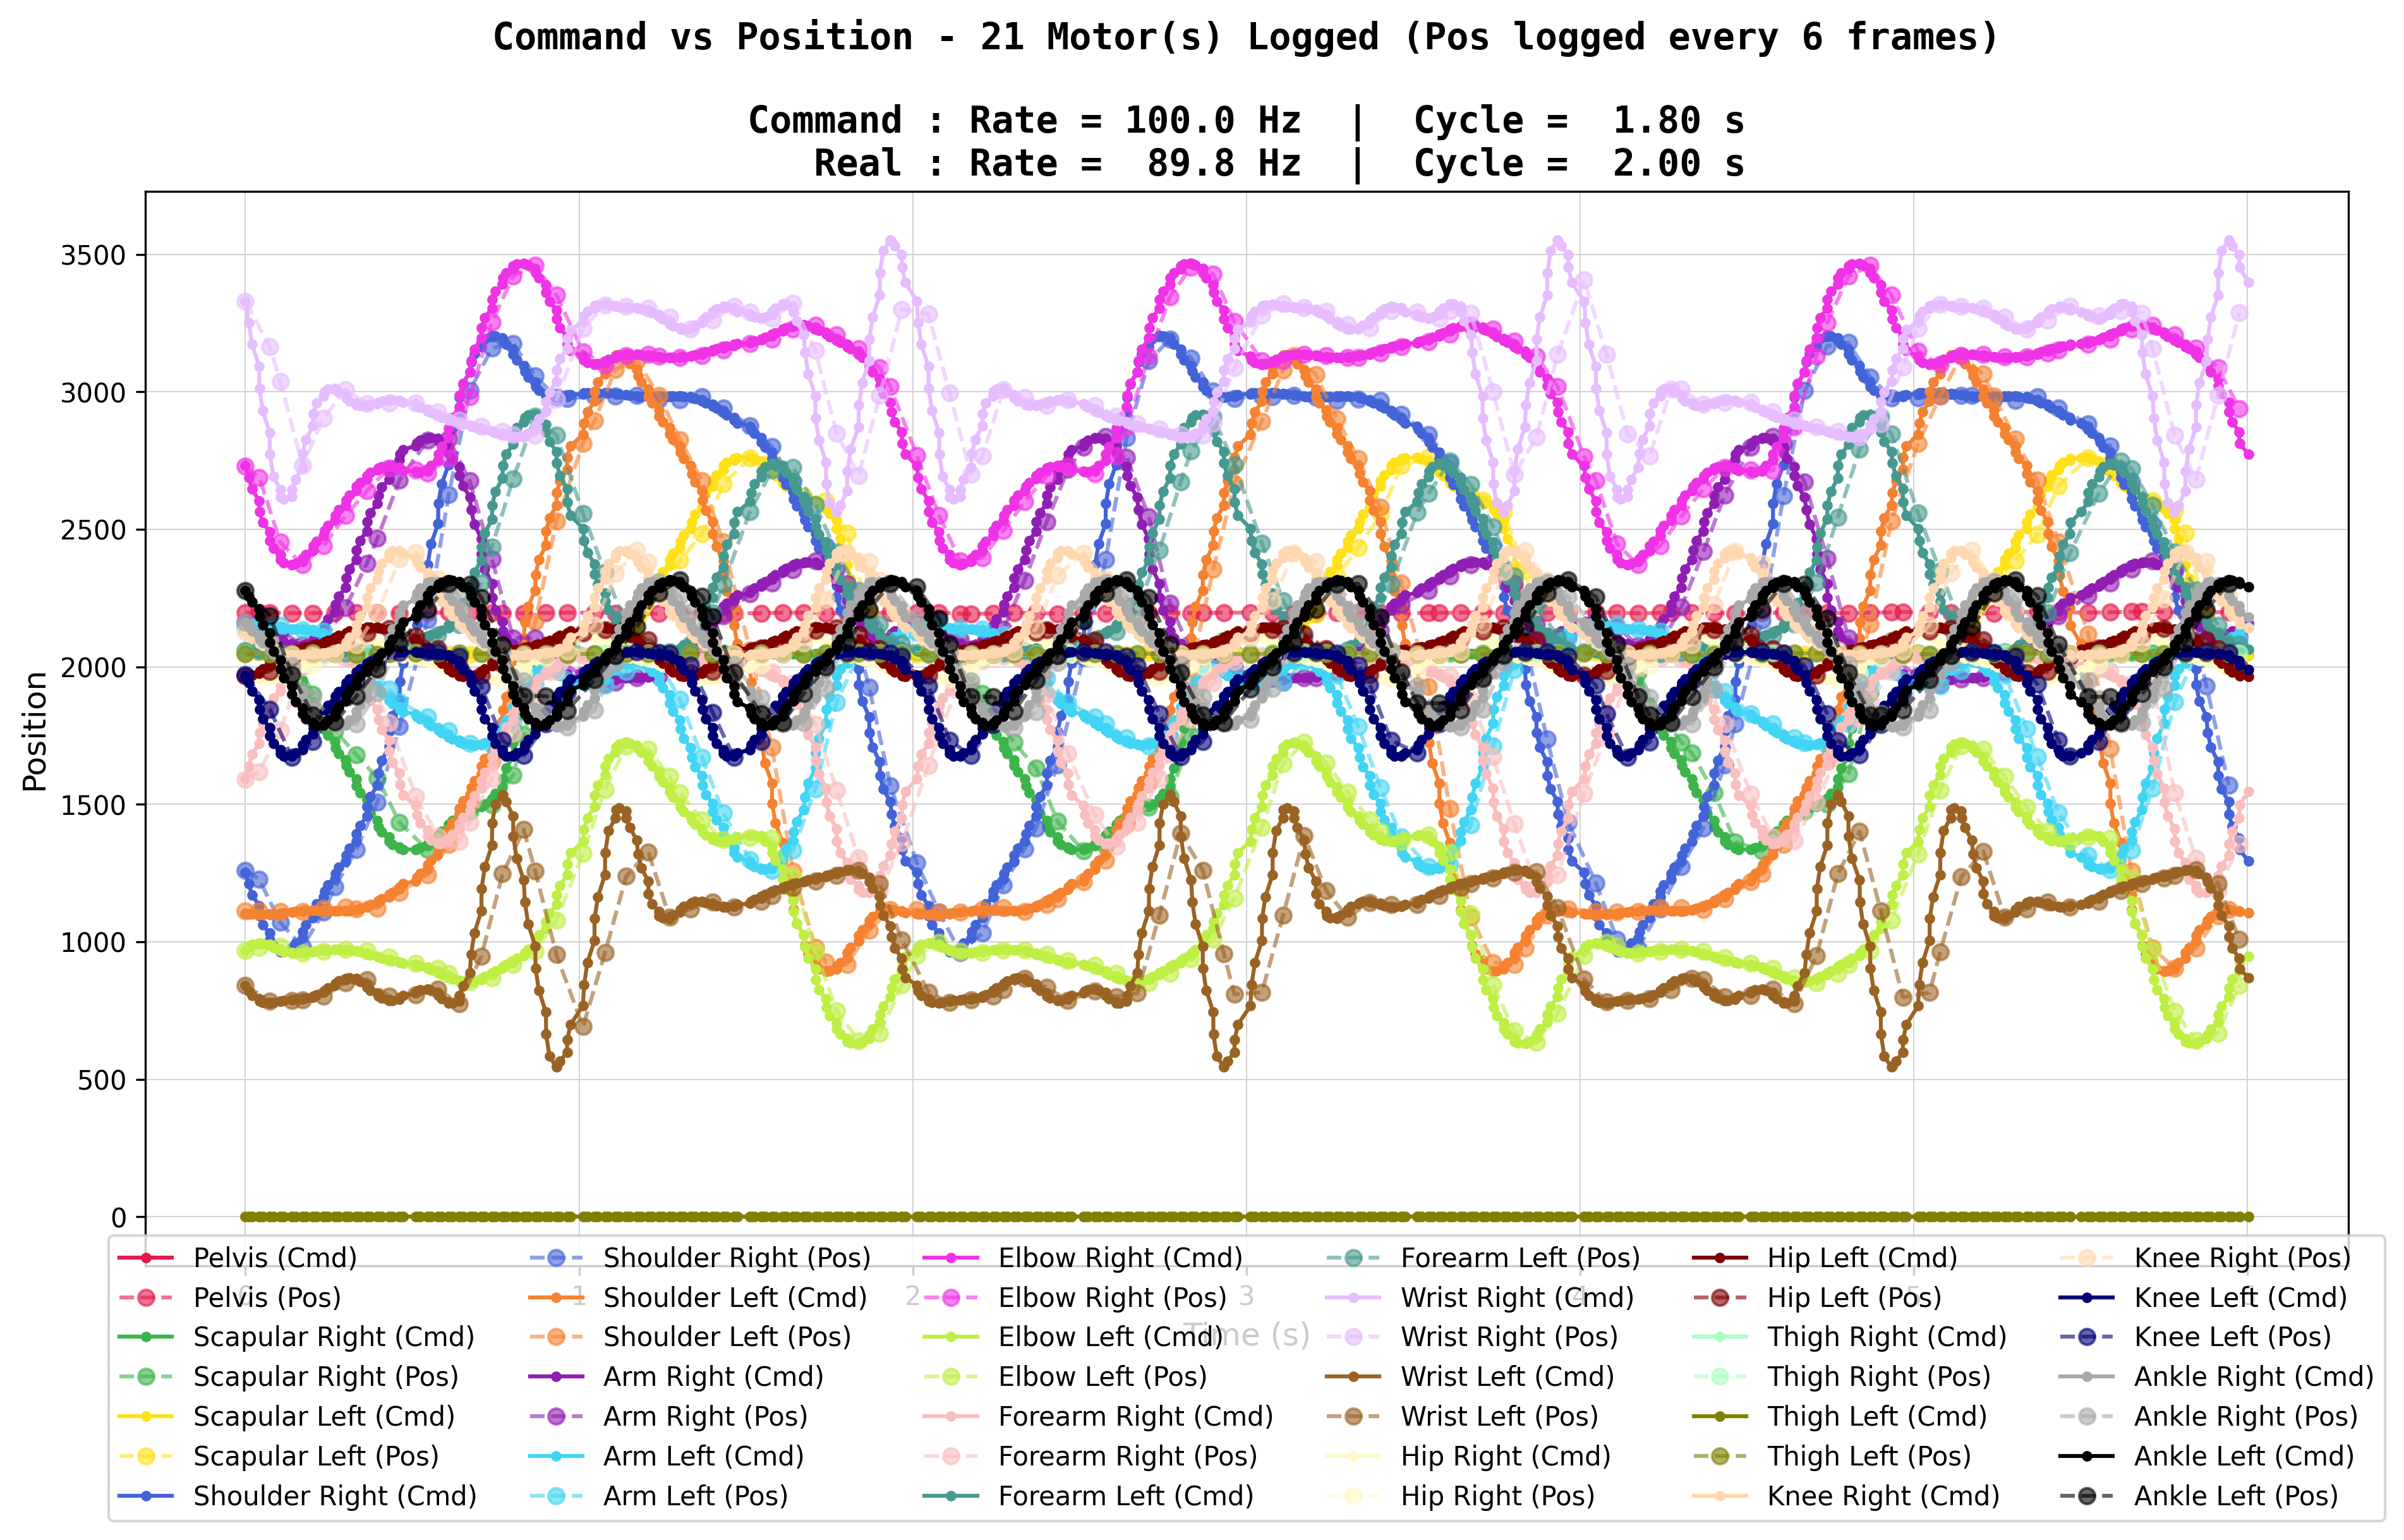
\includegraphics[width=\textwidth]{graphiques_swumanoid/swum_21mot_6f_cmd1p80.png}
        \caption{Commanded cycle 1.80\,s $\rightarrow$ real \textbf{2.00\,s} (89.8 Hz).}
        \label{fig:swum_best}
    \end{subfigure}
    \hfill
    \begin{subfigure}[b]{0.48\textwidth}
        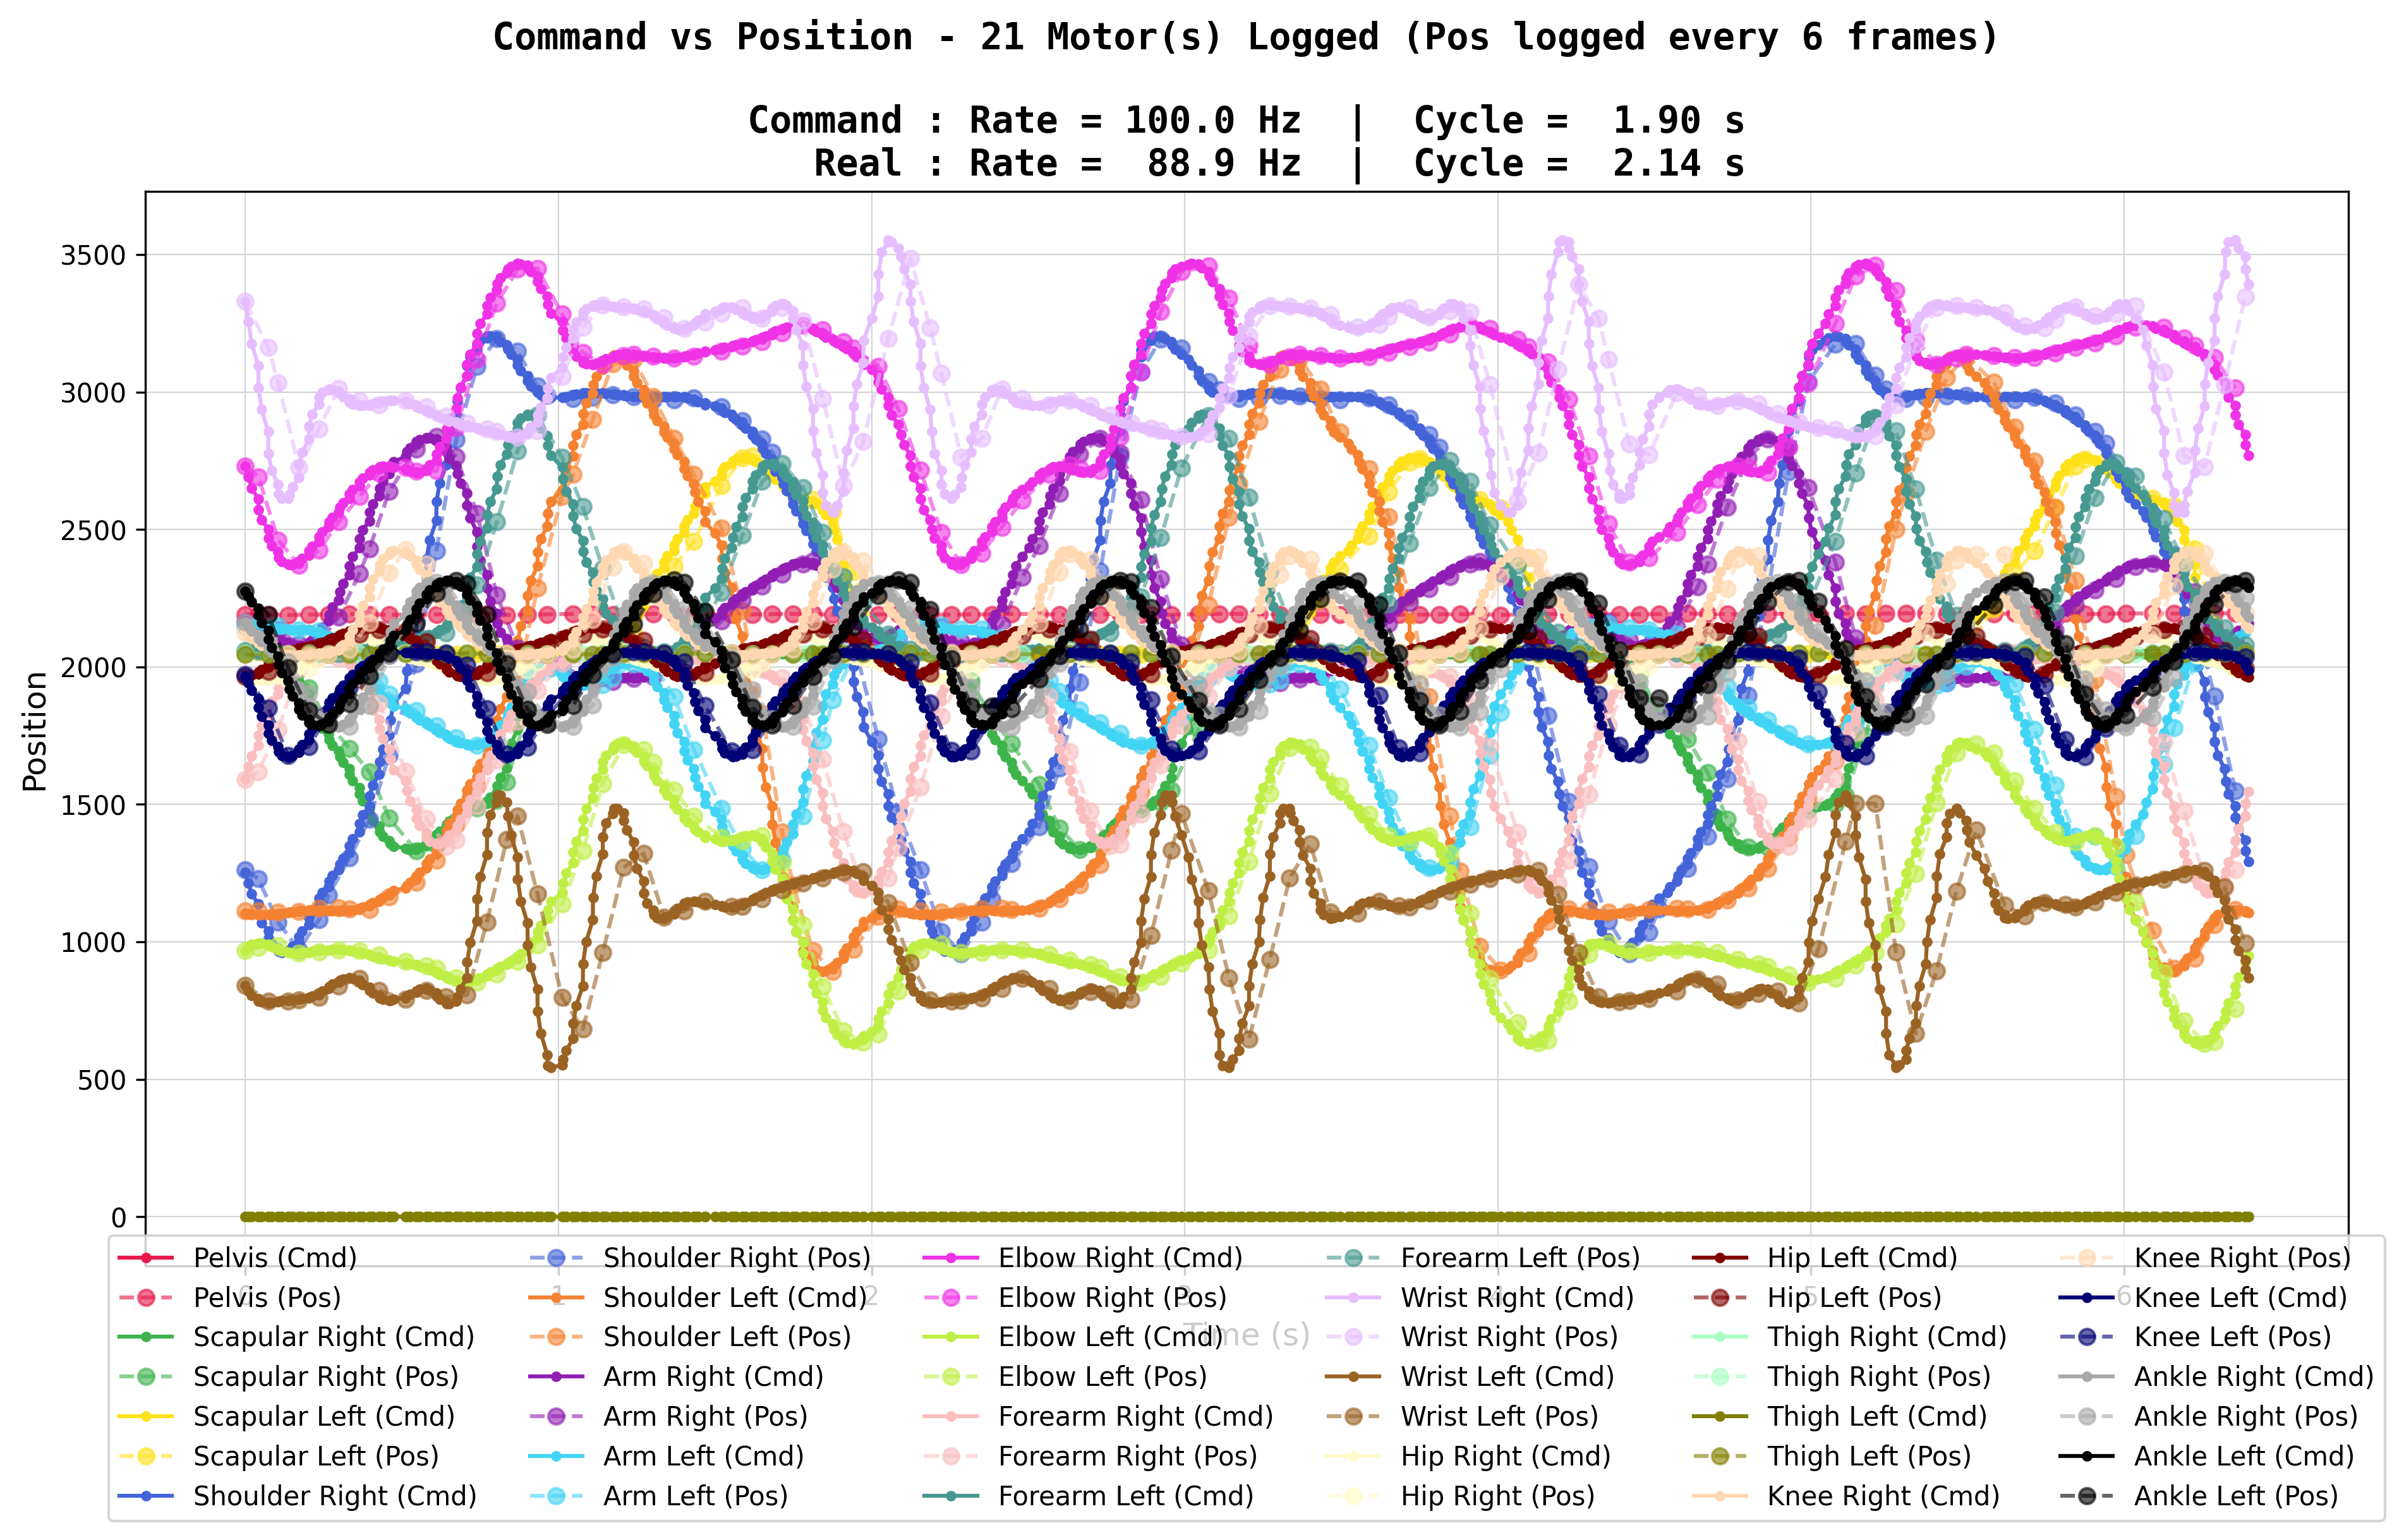
\includegraphics[width=\textwidth]{graphiques_swumanoid/swum_21mot_6f_cmd1p90.png}
        \caption{Commanded cycle 1.90\,s $\rightarrow$ real 2.14\,s (88.9 Hz).}
    \end{subfigure}

    \vspace{0.35em}
    \begin{subfigure}[b]{0.48\textwidth}
        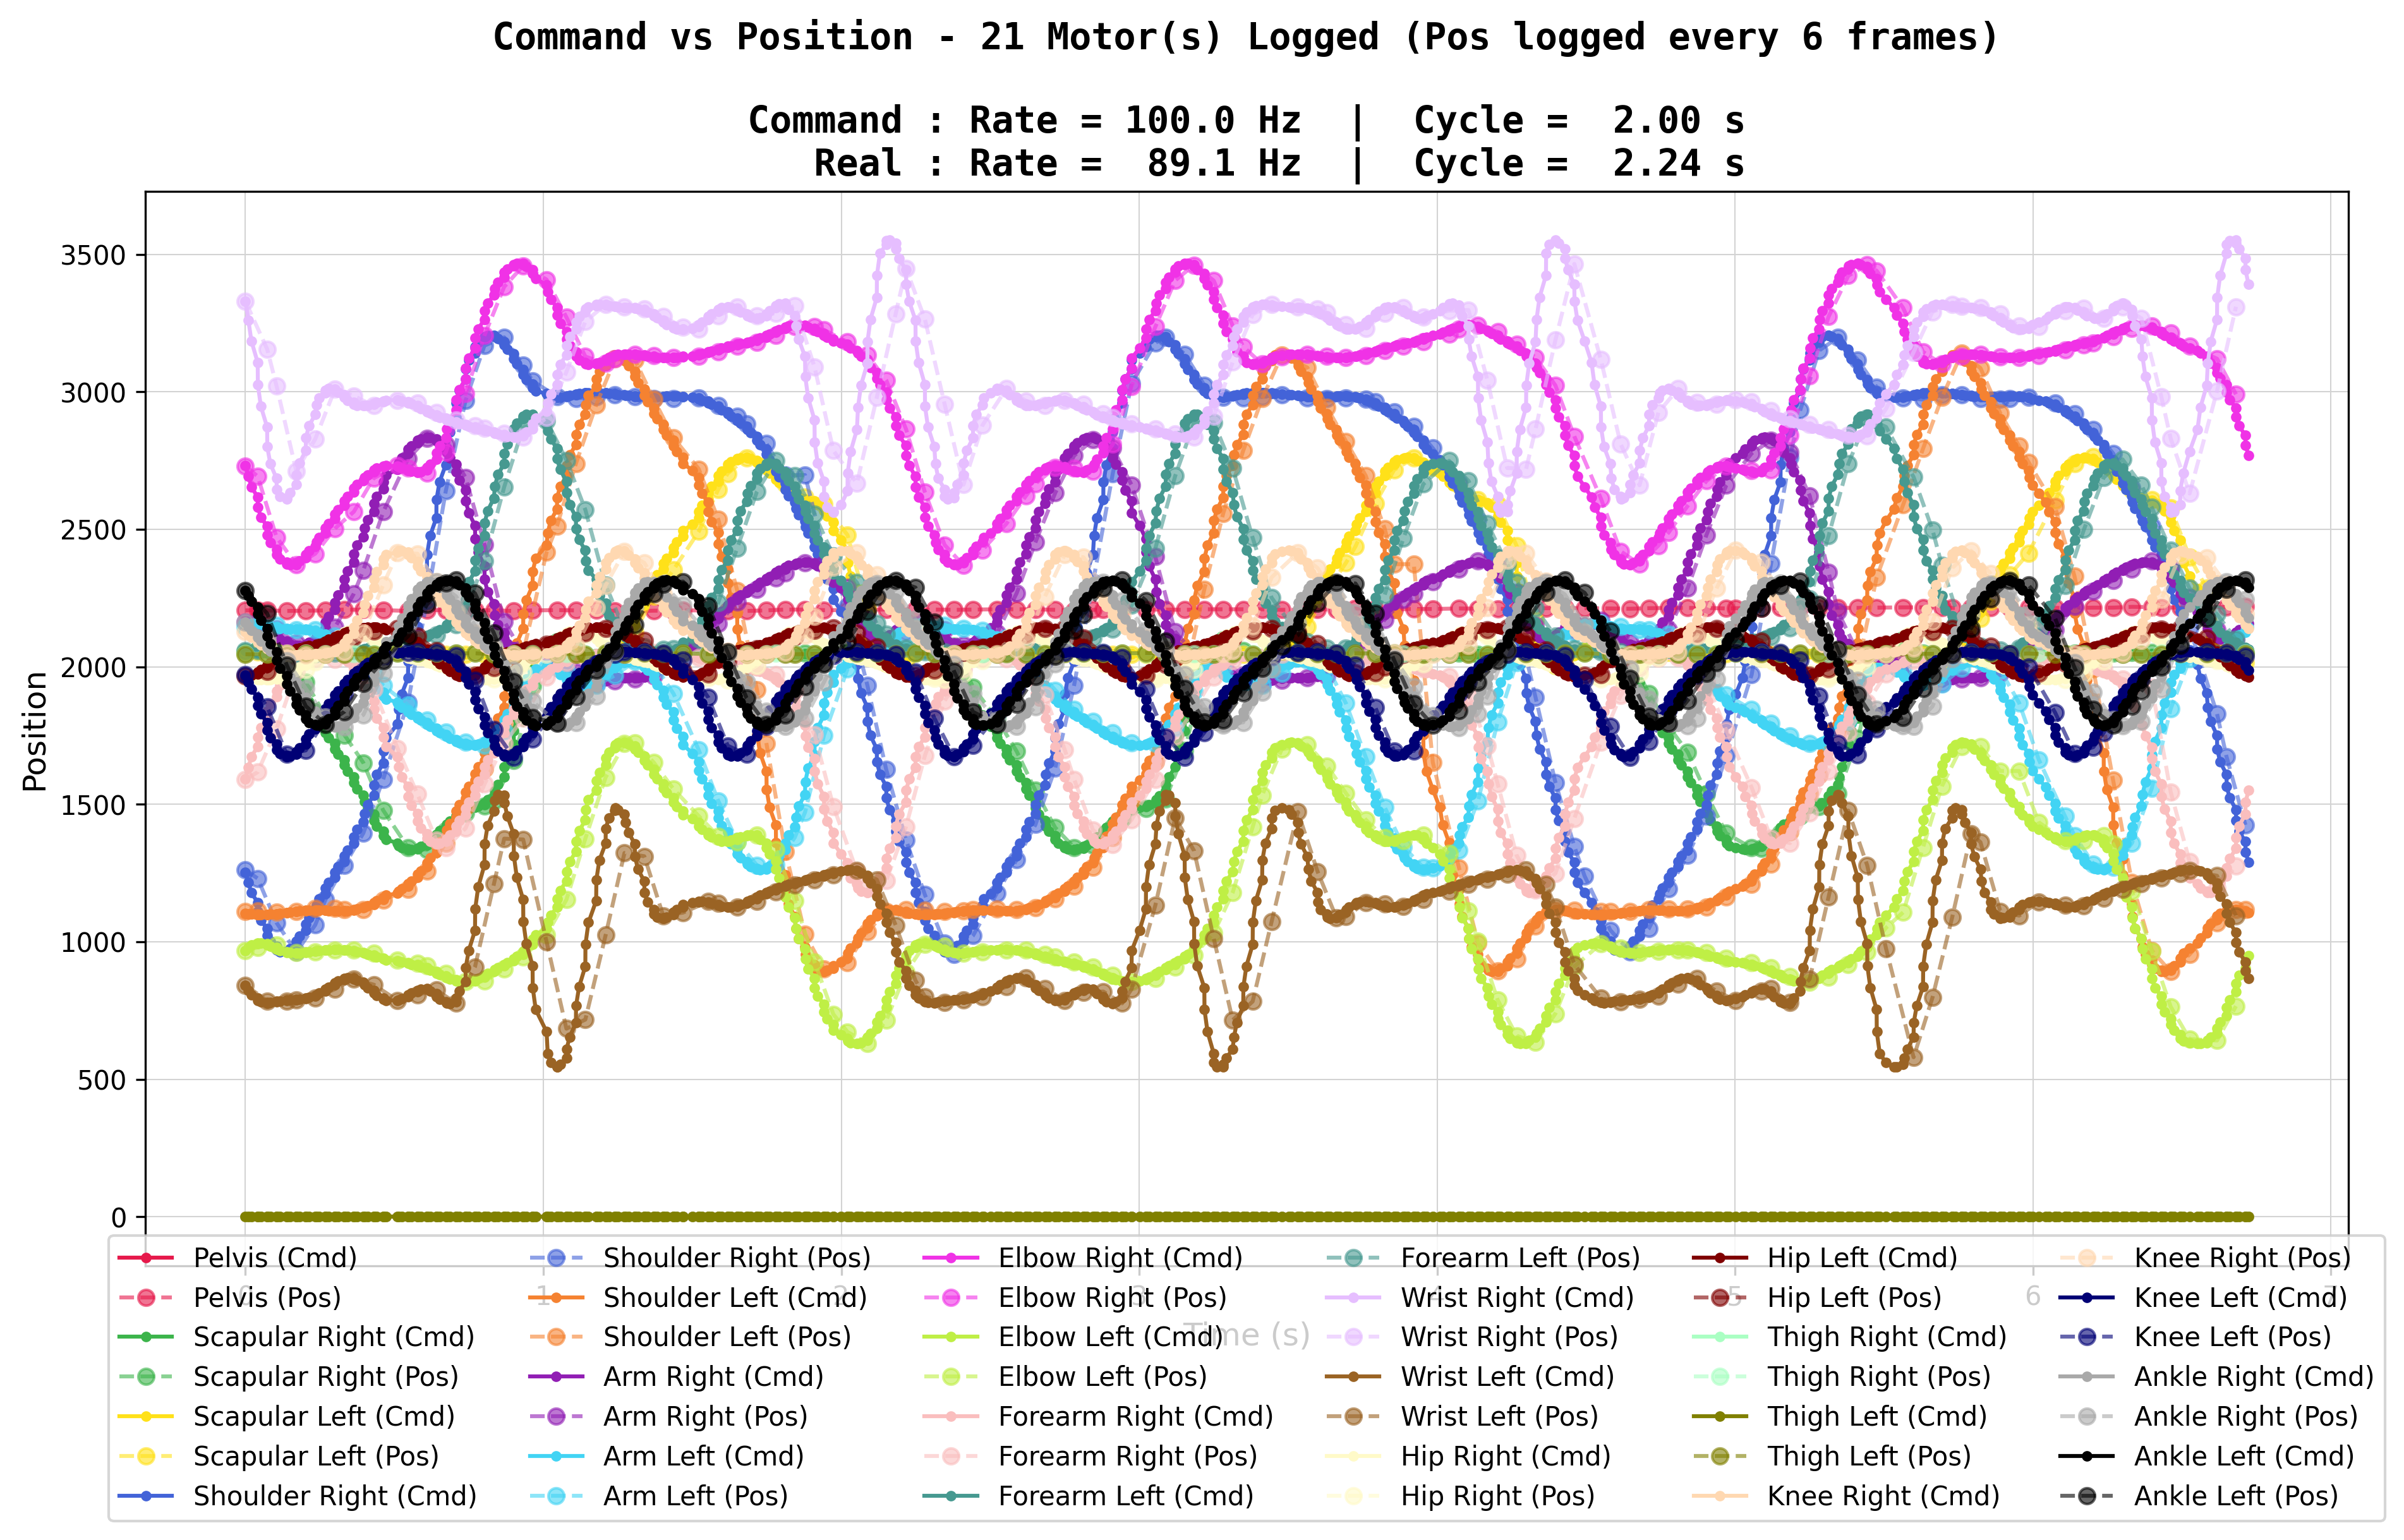
\includegraphics[width=\textwidth]{graphiques_swumanoid/swum_21mot_6f_cmd2p00.png}
        \caption{Commanded cycle 2.00\,s $\rightarrow$ real 2.24\,s (89.1 Hz).}
    \end{subfigure}
    \hfill
    \begin{subfigure}[b]{0.48\textwidth}
        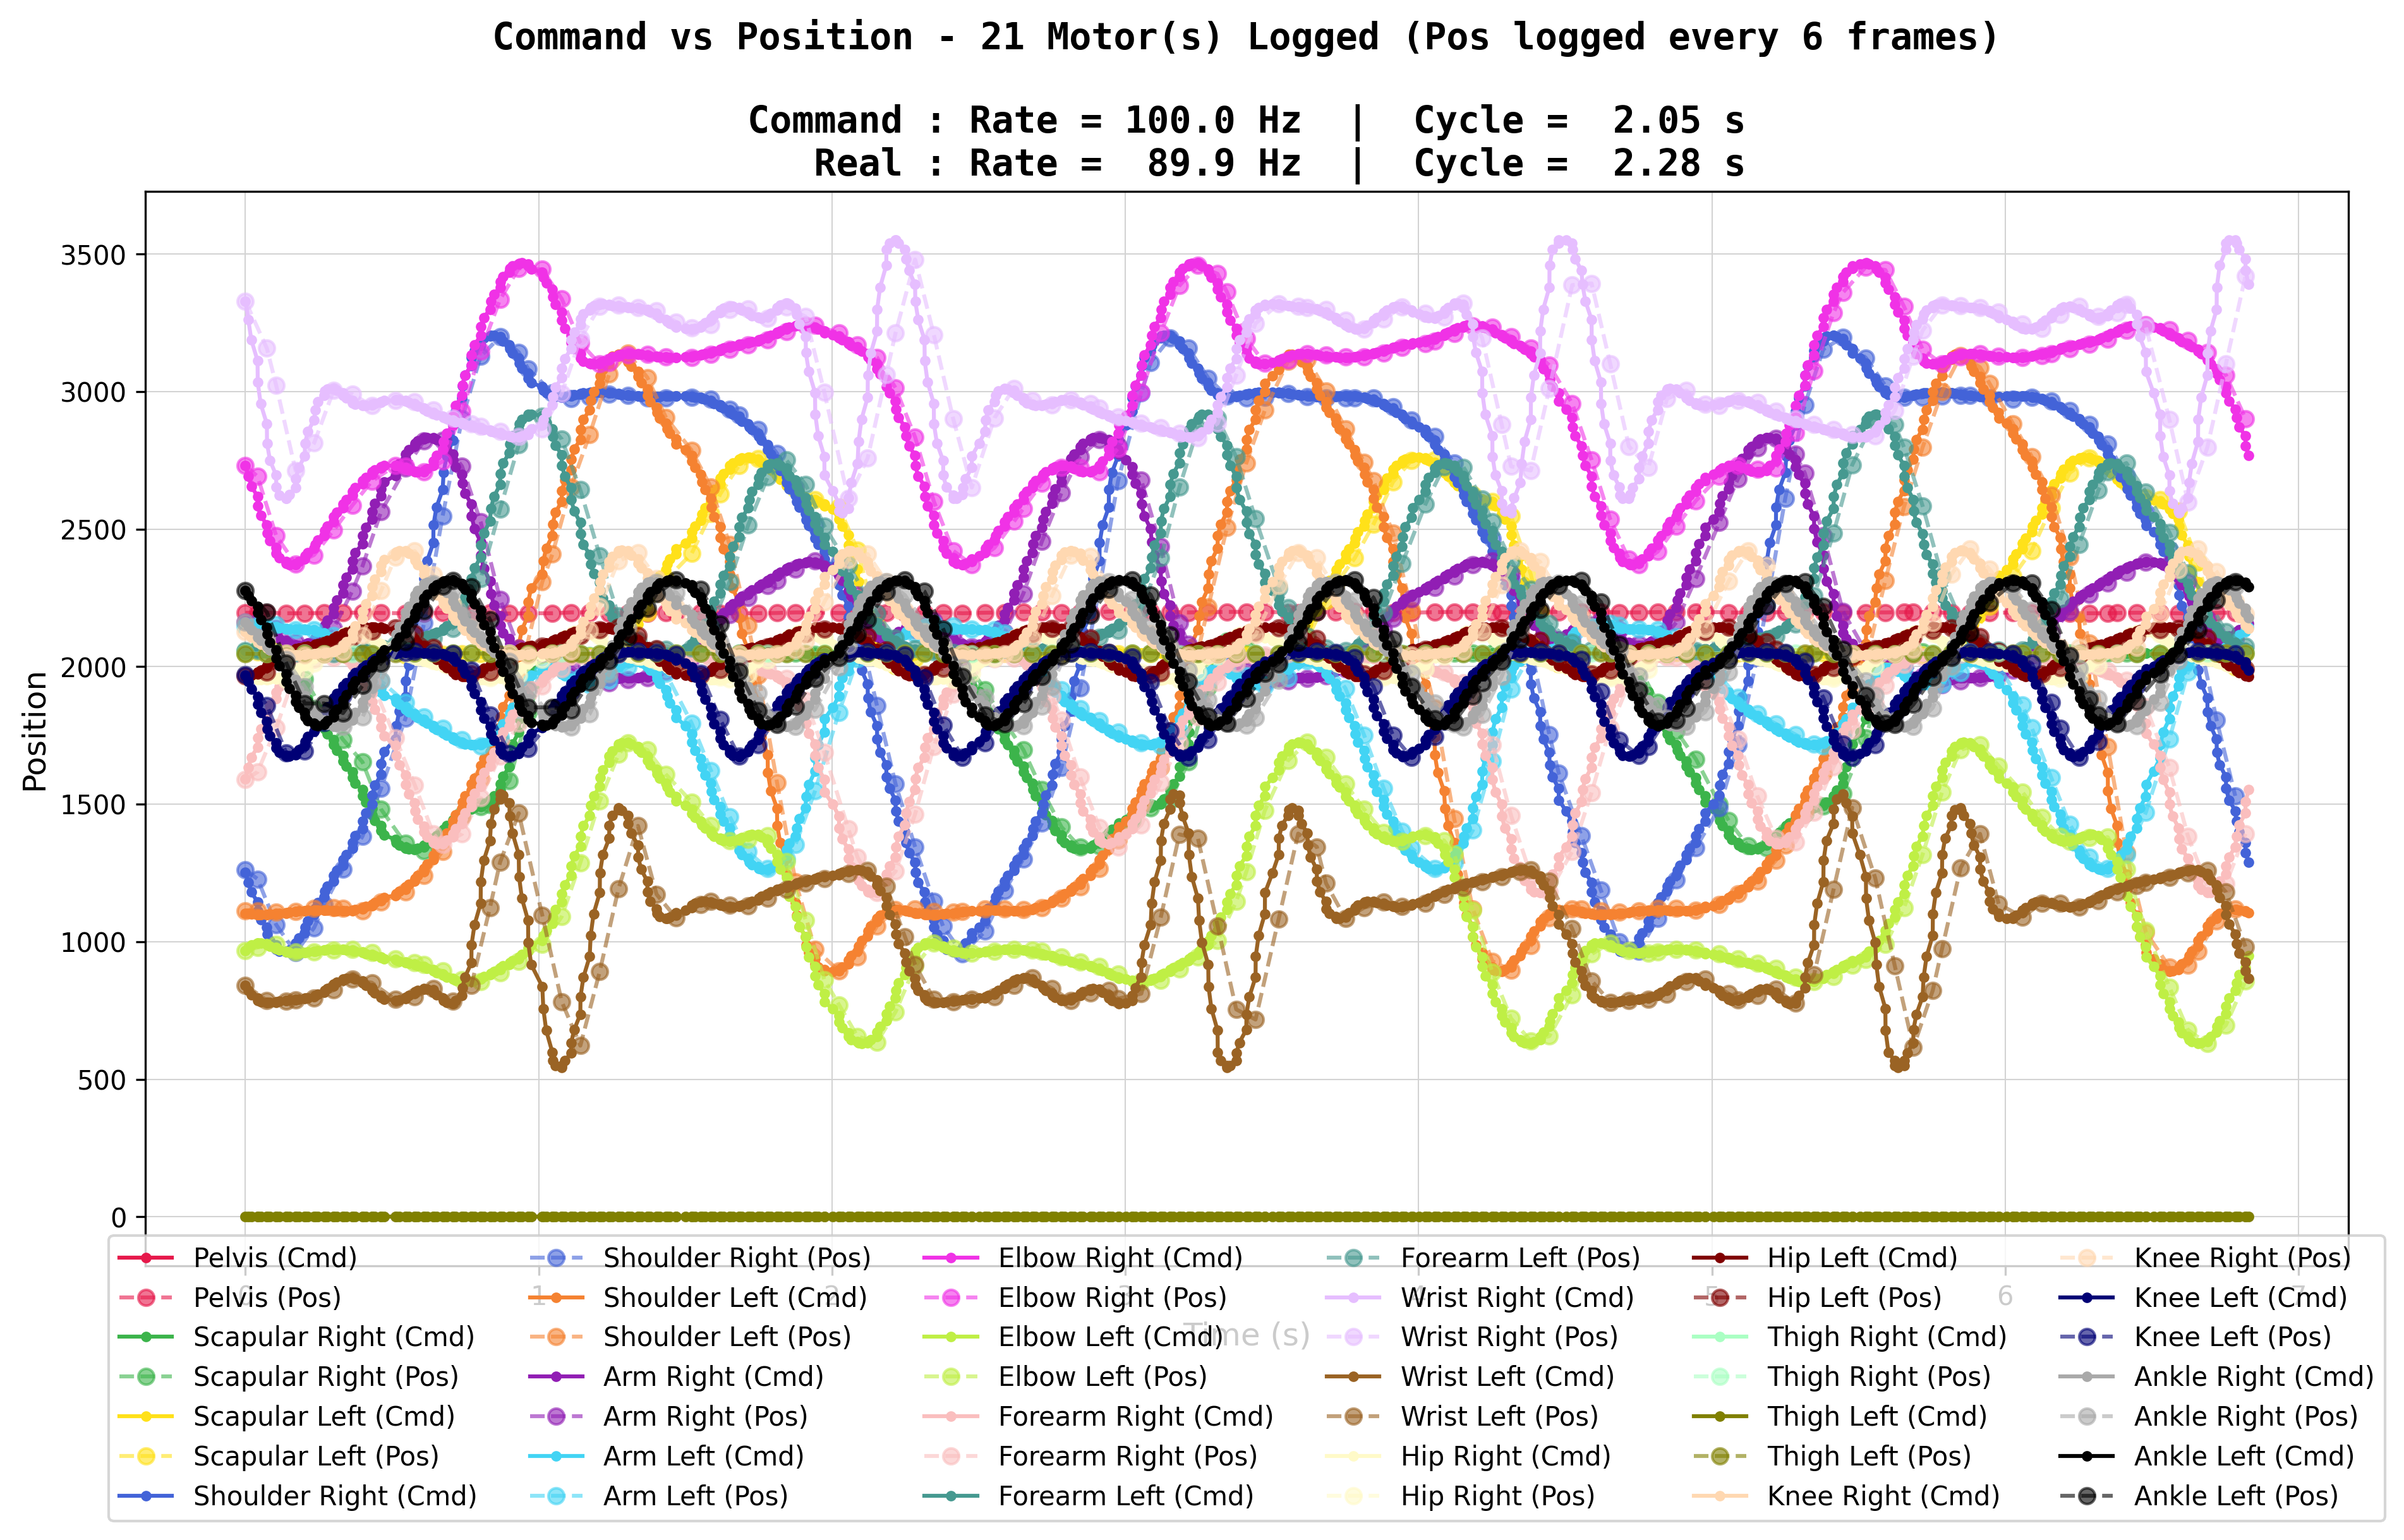
\includegraphics[width=\textwidth]{graphiques_swumanoid/swum_21mot_6f.png}
        \caption{Commanded cycle 2.05\,s $\rightarrow$ real 2.28\,s (89.9 Hz).}
    \end{subfigure}
    \caption{Sweep of the commanded cycle time (100\,Hz, 21 motors, sampling every 6 frames).}
    \label{fig:swum_cycle}
\end{figure}



 The observation confirms that the real frequency stays \emph{invariant}, locked around 89--90\,Hz, whatever the cycle time. The cycle time changes only the total duration, not the rate and it then becomes possible to \emph{pre-compensate} for the known deficit. To obtain the physically targeted swimming cycle of 2.0\,s, we just command a shorter cycle of 1.80\,s, which, stretched by the $1/0.90$ factor, gives exactly 2.00\,s real. This is the best operating point.


\begin{table}[H]
\centering
\begin{tabular}{|c|c|c|c|}
\hline
Commanded cycle (s) & Frames & Real cycle (s) & $f_{\text{real}}$ (Hz) \\ \hline
\textbf{1.80} & 180 & \textbf{2.00} & 89.8 \\ \hline
1.90 & 190 & 2.14 & 88.9 \\ \hline
2.00 & 200 & 2.24 & 89.1 \\ \hline
2.05 & 205 & 2.28 & 89.9 \\ \hline
\end{tabular}
\caption{Sweep of the cycle time at 21 logged motors (every 6 frames, 100\,Hz).}
\label{tab:swum_cycle}
\end{table}

The real frequency is invariant ($\approx 89.4 \pm 0.5$\,Hz) and $\text{real cycle} = \text{commanded cycle} \times 100/f_{\text{real}}$. Furthermore, we can see in the table that the 1.80\,s setting hits the target swimming cycle of 2.00\,s.

This campaign on the real robot fully confirms the budget model and leads to a parameter set determined by experiment, which will serve as the reference for the future swimming experiments. 
 
\paragraph{Optimal parameters retained :}
\begin{itemize}
    \item \textbf{Command rate}: 100\,Hz.
    \item \textbf{Logged motors}: 21, the whole body.
    \item \textbf{Sampling interval}: 6 frames.
    \item \textbf{Commanded cycle time}: 1.80\,s.
    \item \textbf{Real control rate}: $\approx 90$\,Hz.
\end{itemize}
This setting brings together the full telemetry of the 21 joints, a high and faithful control rate, and a real swimming cycle exactly matching the physical setpoint. It is the operating base on which the swimming-dynamics analyses that follow will rely.


\section{Motion Kinematics and Interpolation}
\label{sec:method_interpolation}

\subsection{The Problem of Previous System}

In the first system, we could'nt change the frequency of control and the number of frames of the motion file. So a linear interpolation was implemented but used to connect the motion frames guaranteed position continuity and not the continuity of its derivatives, so at each node, the commanded velocity changed discontinuously (theoretically infinite acceleration), which produced jerky motion. In particular, during the cyclic playback of a motion, the repetition of the same file, the last frame usually did not coincide with the first and the loop-back caused a jump in position and velocity, and therefore a mechanical jolt at every cycle start. 

Before developping this section we can notice that, although the new hardware configuration (described in Section \ref{sec:motors_board_configuration}) allows control at 200 Hz, its development took significant time to design and deliver. During that wait, the pool tests had to run on the old configuration, capped at very low frequencies (between 36 Hz and 50 Hz) because of a low baud rate. But this temporary hardware constraint made us aware of some flaws in our algorithm. In fact at high frequency the density of command points hides the mathematical interpolation errors but at low frequency, though, the trajectory's continuity defects become large and physically destructive for the robot's swimming.

Moreover, the move to the initial pose was also too abrupt, and a software bug froze the control frequency at 15~Hz regardless of the interface settings.

To gain full flexibility over the timing, as explained in the previous section, the parameter management logic was inverted. From now on, the control frequency $f_{\mathrm{c}}$, the cycle duration $T_{\mathrm{cycle}}$ and the number of repetitions $N_{\mathrm{plays}}$ are the only variables set by the user. The number of frames per cycle $F$ is no longer a constraint imposed by the source file, but a variable computed dynamically:

\begin{equation}
    F = f_{\mathrm{c}} \times T_{\mathrm{cycle}}
\end{equation}

The time interval between two motor commands is thus fixed at $\Delta t = 1/f_{\mathrm{c}}$. Since $F$ generally differs from the number of points $N$ in the motion file, new joint positions must be recomputed to match this exact time grid and so that is the role of interpolation.

\subsection{Choosing the Cubic Spline}

We used first the piecewise-linear interpolation which is only class $\mathcal{C}^0$ so the velocity is piecewise constant and discontinuous at the nodes, which forces the motors into "staircase" command changes. To solve this issue, and as used by M. NAKASHIMA in the SWUM simulation \cite{nakashima2012optimizing}, we replaced it with a \textit{periodic cubic spline}, a piecewise polynomial function of degree~3, class $\mathcal{C}^2$ over the whole interval, it means the interpolated position, velocity \emph{and} acceleration are continuous at the nodes. The acceleration discontinuities are thus eliminated at the source, for a compute cost linear in $N$.

The $N$ frames of the source file are indexed on a uniform grid $x_i = i$, $i = 0,\dots,N-1$ (step $h = x_{i+1} - x_i = 1$), and we write $y_i$ for the angular command of a joint at frame $i$. We can notice that each motor is handled independently by the same algorithm. On each interval $[x_i,\, x_{i+1}]$ of uniform step $h = x_{i+1} - x_i$, the trajectory is modeled by a cubic polynomial:
\begin{equation}
    S_i(x) = a_i + b_i\,(x - x_i) + c_i\,(x - x_i)^2 + d_i\,(x - x_i)^3
    \qquad \text{with} \quad x \in [x_i,\, x_{i+1}]
    \label{eq:spline-cubique}
\end{equation}

Because $S_i(x)$ is a polynomial of degree~3, its second derivative $S''_i(x)$ is strictly linear on the interval. We can therefore express it directly using linear interpolation between the second derivatives at the nodes, $y''_i = S''_i(x_i)$ and $y''_{i+1} = S''_i(x_{i+1})$. Introducing the barycentric coordinates  and  yields:
\begin{equation}
    S''_i(x) = A\,y''_i + B\,y''_{i+1} \quad \text{with} \quad A = \frac{x_{i+1} - x}{h} \quad \text{and} \quad B = 1 - A = \frac{x - x_i}{h}
\end{equation}

Integrating this expression twice introduces two integration constants, $C_1$ and $C_2$:
\begin{equation}
    S_i(x) = \frac{h^2}{6}\,A^3\,y''_i + \frac{h^2}{6}\,B^3\,y''_{i+1} + C_1\,A + C_2\,B
\end{equation}

Enforcing the $\mathcal{C}^0$ positional boundary conditions at the nodes ($S_i(x_i) = y_i$ at $A=1, B=0$, and $S_i(x_{i+1}) = y_{i+1}$ at $A=0, B=1$) determines these constants as $C_1 = y_i - \frac{h^2}{6}y''_i$ and $C_2 = y_{i+1} - \frac{h^2}{6}y''_{i+1}$. Substituting them back into the expression gives the barycentric formulation:
\begin{equation}
    S_i(x) = A\,y_i + B\,y_{i+1}
    + \frac{h^2}{6}\left[(A^3 - A)\,y''_i + (B^3 - B)\,y''_{i+1}\right]
    \label{eq:spline-nr}
\end{equation}

By construction, this formulation inherently satisfies nodal interpolation and $\mathcal{C}^2$ continuity. The coefficients of the canonical form~\eqref{eq:spline-cubique} are then determined by evaluating $S_i$ and its successive derivatives at the node $x = x_i$ ($A=1, B=0$):
\begin{itemize}
    \item \textbf{Position ($a_i$)}: $S_i(x_i) = a_i = y_i$
    \item \textbf{Second derivative ($c_i$)}: $S''_i(x_i) = 2c_i = y''_i \implies c_i = \frac{y''_i}{2}$
    \item \textbf{Third derivative ($d_i$)}: Differentiating $S''_i(x)$ yields $S'''_i(x_i) = 6d_i = \frac{y''_{i+1} - y''_i}{h} \implies d_i = \frac{y''_{i+1} - y''_i}{6h}$
    \item \textbf{First derivative ($b_i$)}: Differentiating~\eqref{eq:spline-nr} with respect to $x$ (using $\frac{\mathrm{d}A}{\mathrm{d}x} = -\frac{1}{h}$ and $\frac{\mathrm{d}B}{\mathrm{d}x} = \frac{1}{h}$) and evaluating at $x_i$ gives $S'_i(x_i) = b_i = \frac{y_{i+1} - y_i}{h} - \frac{h}{6}(2y''_i + y''_{i+1})$.
\end{itemize}

This provides the exact coefficient set for the trajectory segment :
\begin{equation}
    a_i = y_i, \qquad
    b_i = \frac{y_{i+1} - y_i}{h} - \frac{h}{6}\left(2y''_i + y''_{i+1}\right), \qquad
    c_i = \frac{y''_i}{2}, \qquad
    d_i = \frac{y''_{i+1} - y''_i}{6h}
    \label{eq:spline-coeffs}
\end{equation}

But before solving the problem, we need to understand the limits of a classic interpolation, where the second derivative is forced to zero at the ends. The SWUMANOID's original motion files are designed for a 2-second cycle at 72~Hz, so 144 frames. To assess this method, let us first look at its behavior at a high control frequency (90~Hz).

\begin{figure}[H]
    \centering
    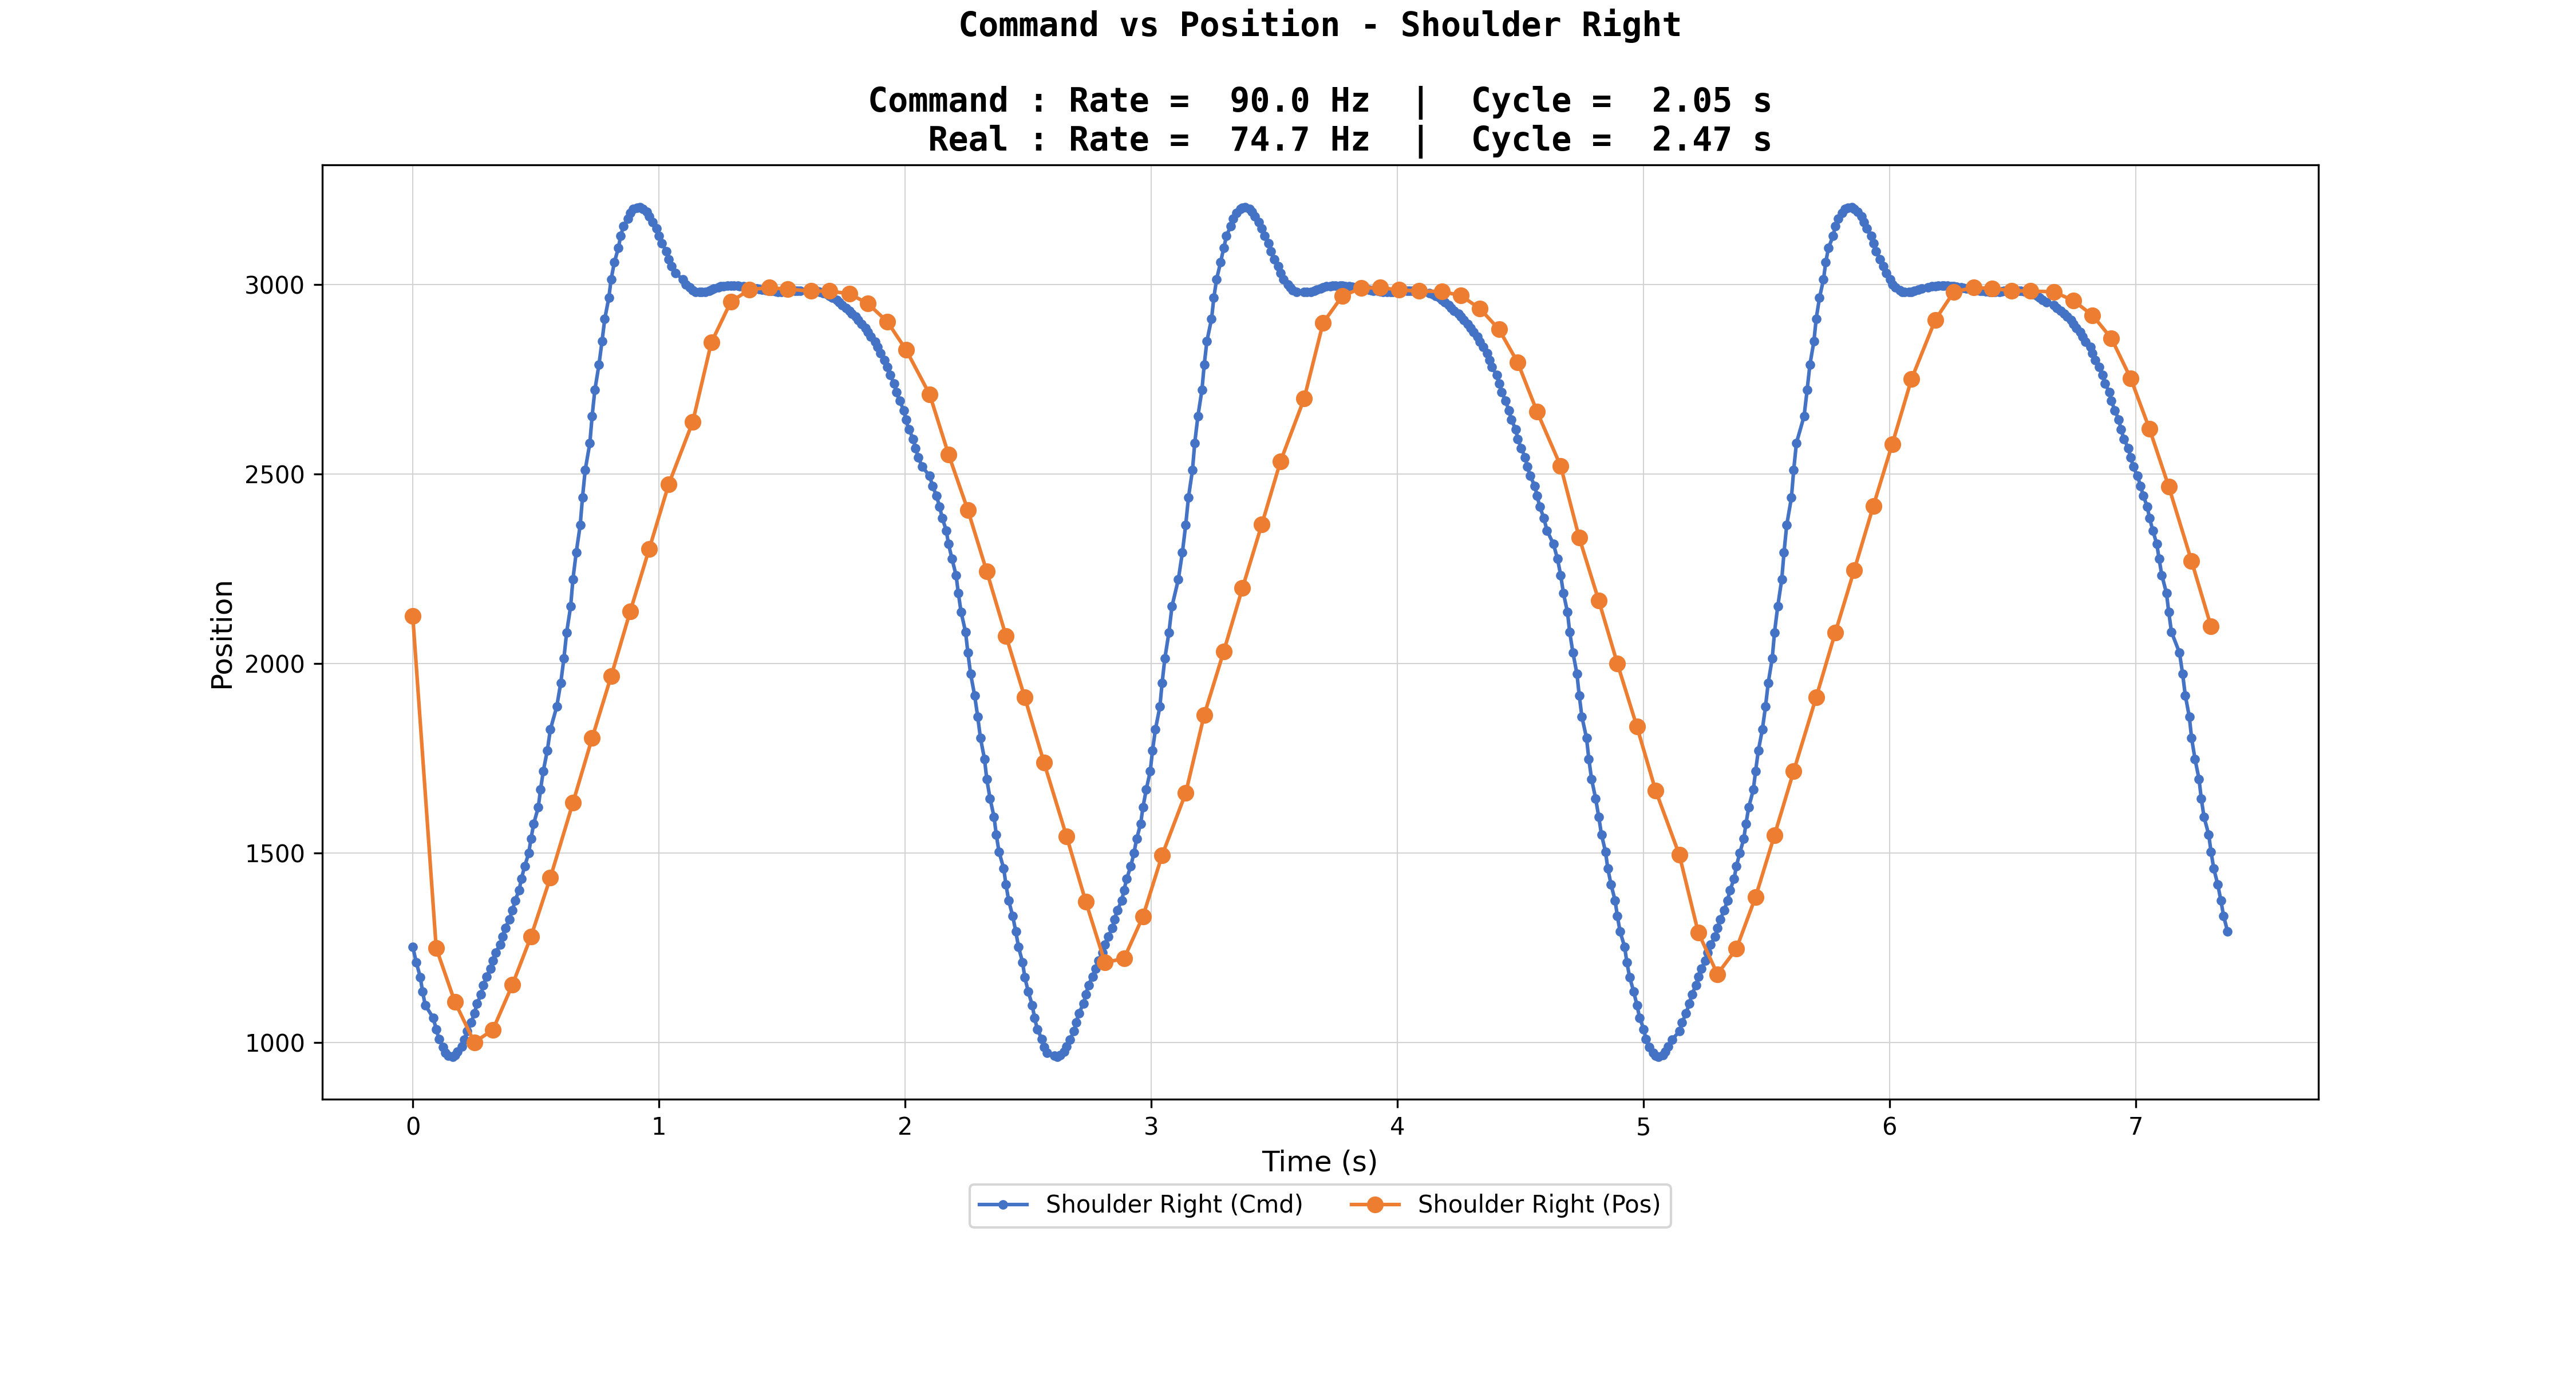
\includegraphics[width=0.8\textwidth]{graphiques/202607141616_ID_4_Spline_Cubic_Pure_90Hz.png}
    \caption{Natural interpolation at 90 Hz.}
    \label{fig:spline_nat_90}
\end{figure}

At that frequency, the number of recomputed points is large, as the figure~\ref{fig:spline_nat_90} shows, the blue command curve follows the trajectory faithfully. The mathematical defect at the ends exists, but the very high density of points almost entirely masks it at the loop-back around 2 seconds. But the fragility of this approach shows up as soon as we move away from the design frequency by subsampling.

\begin{figure}[H]
    \centering
    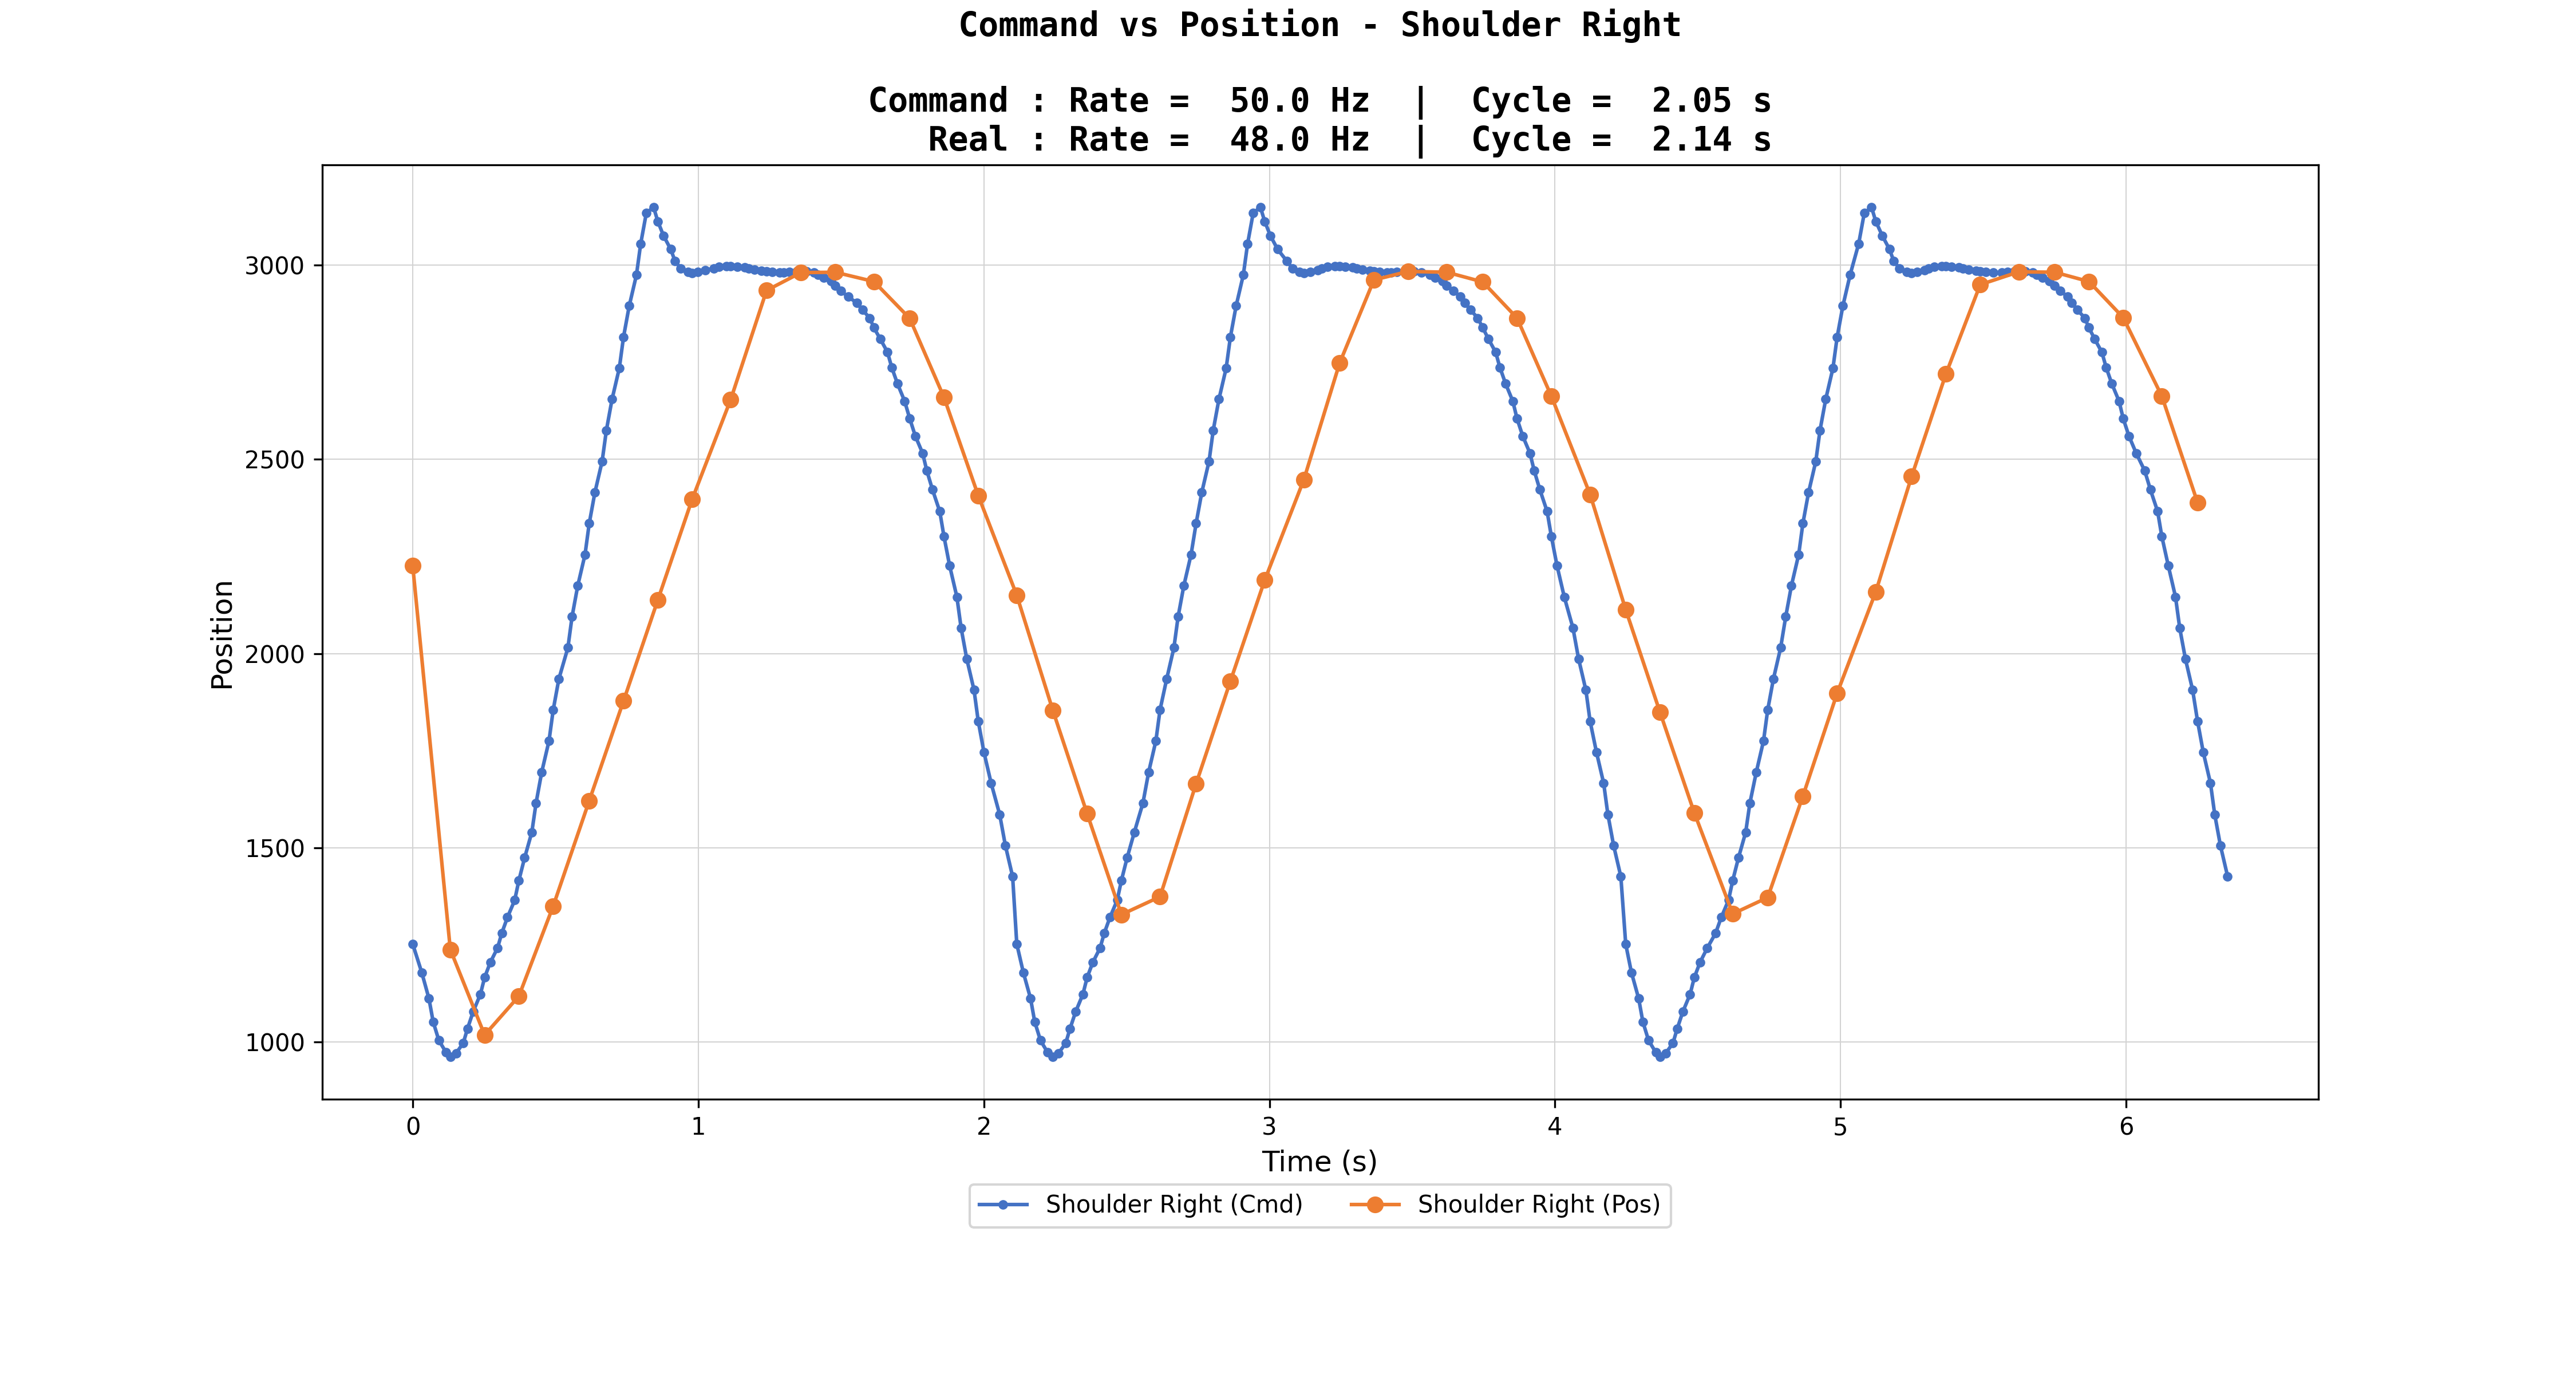
\includegraphics[width=0.8\textwidth]{graphiques/202607141612_ID_4_Spline_Cubic_Pure_50Hz.png}
    \caption{Natural interpolation at 50 Hz.}
    \label{fig:spline_nat_50}
\end{figure}

At 50~Hz, the natural spline starts to reveal its weaknesses, indeed, the plot in the figure~\ref{fig:spline_nat_50} highlights a clearly visible offset at the end of the cycle, the last interpolated frame no longer joins the first frame of the next cycle cleanly, creating a command jump.

\begin{figure}[H]
    \centering
    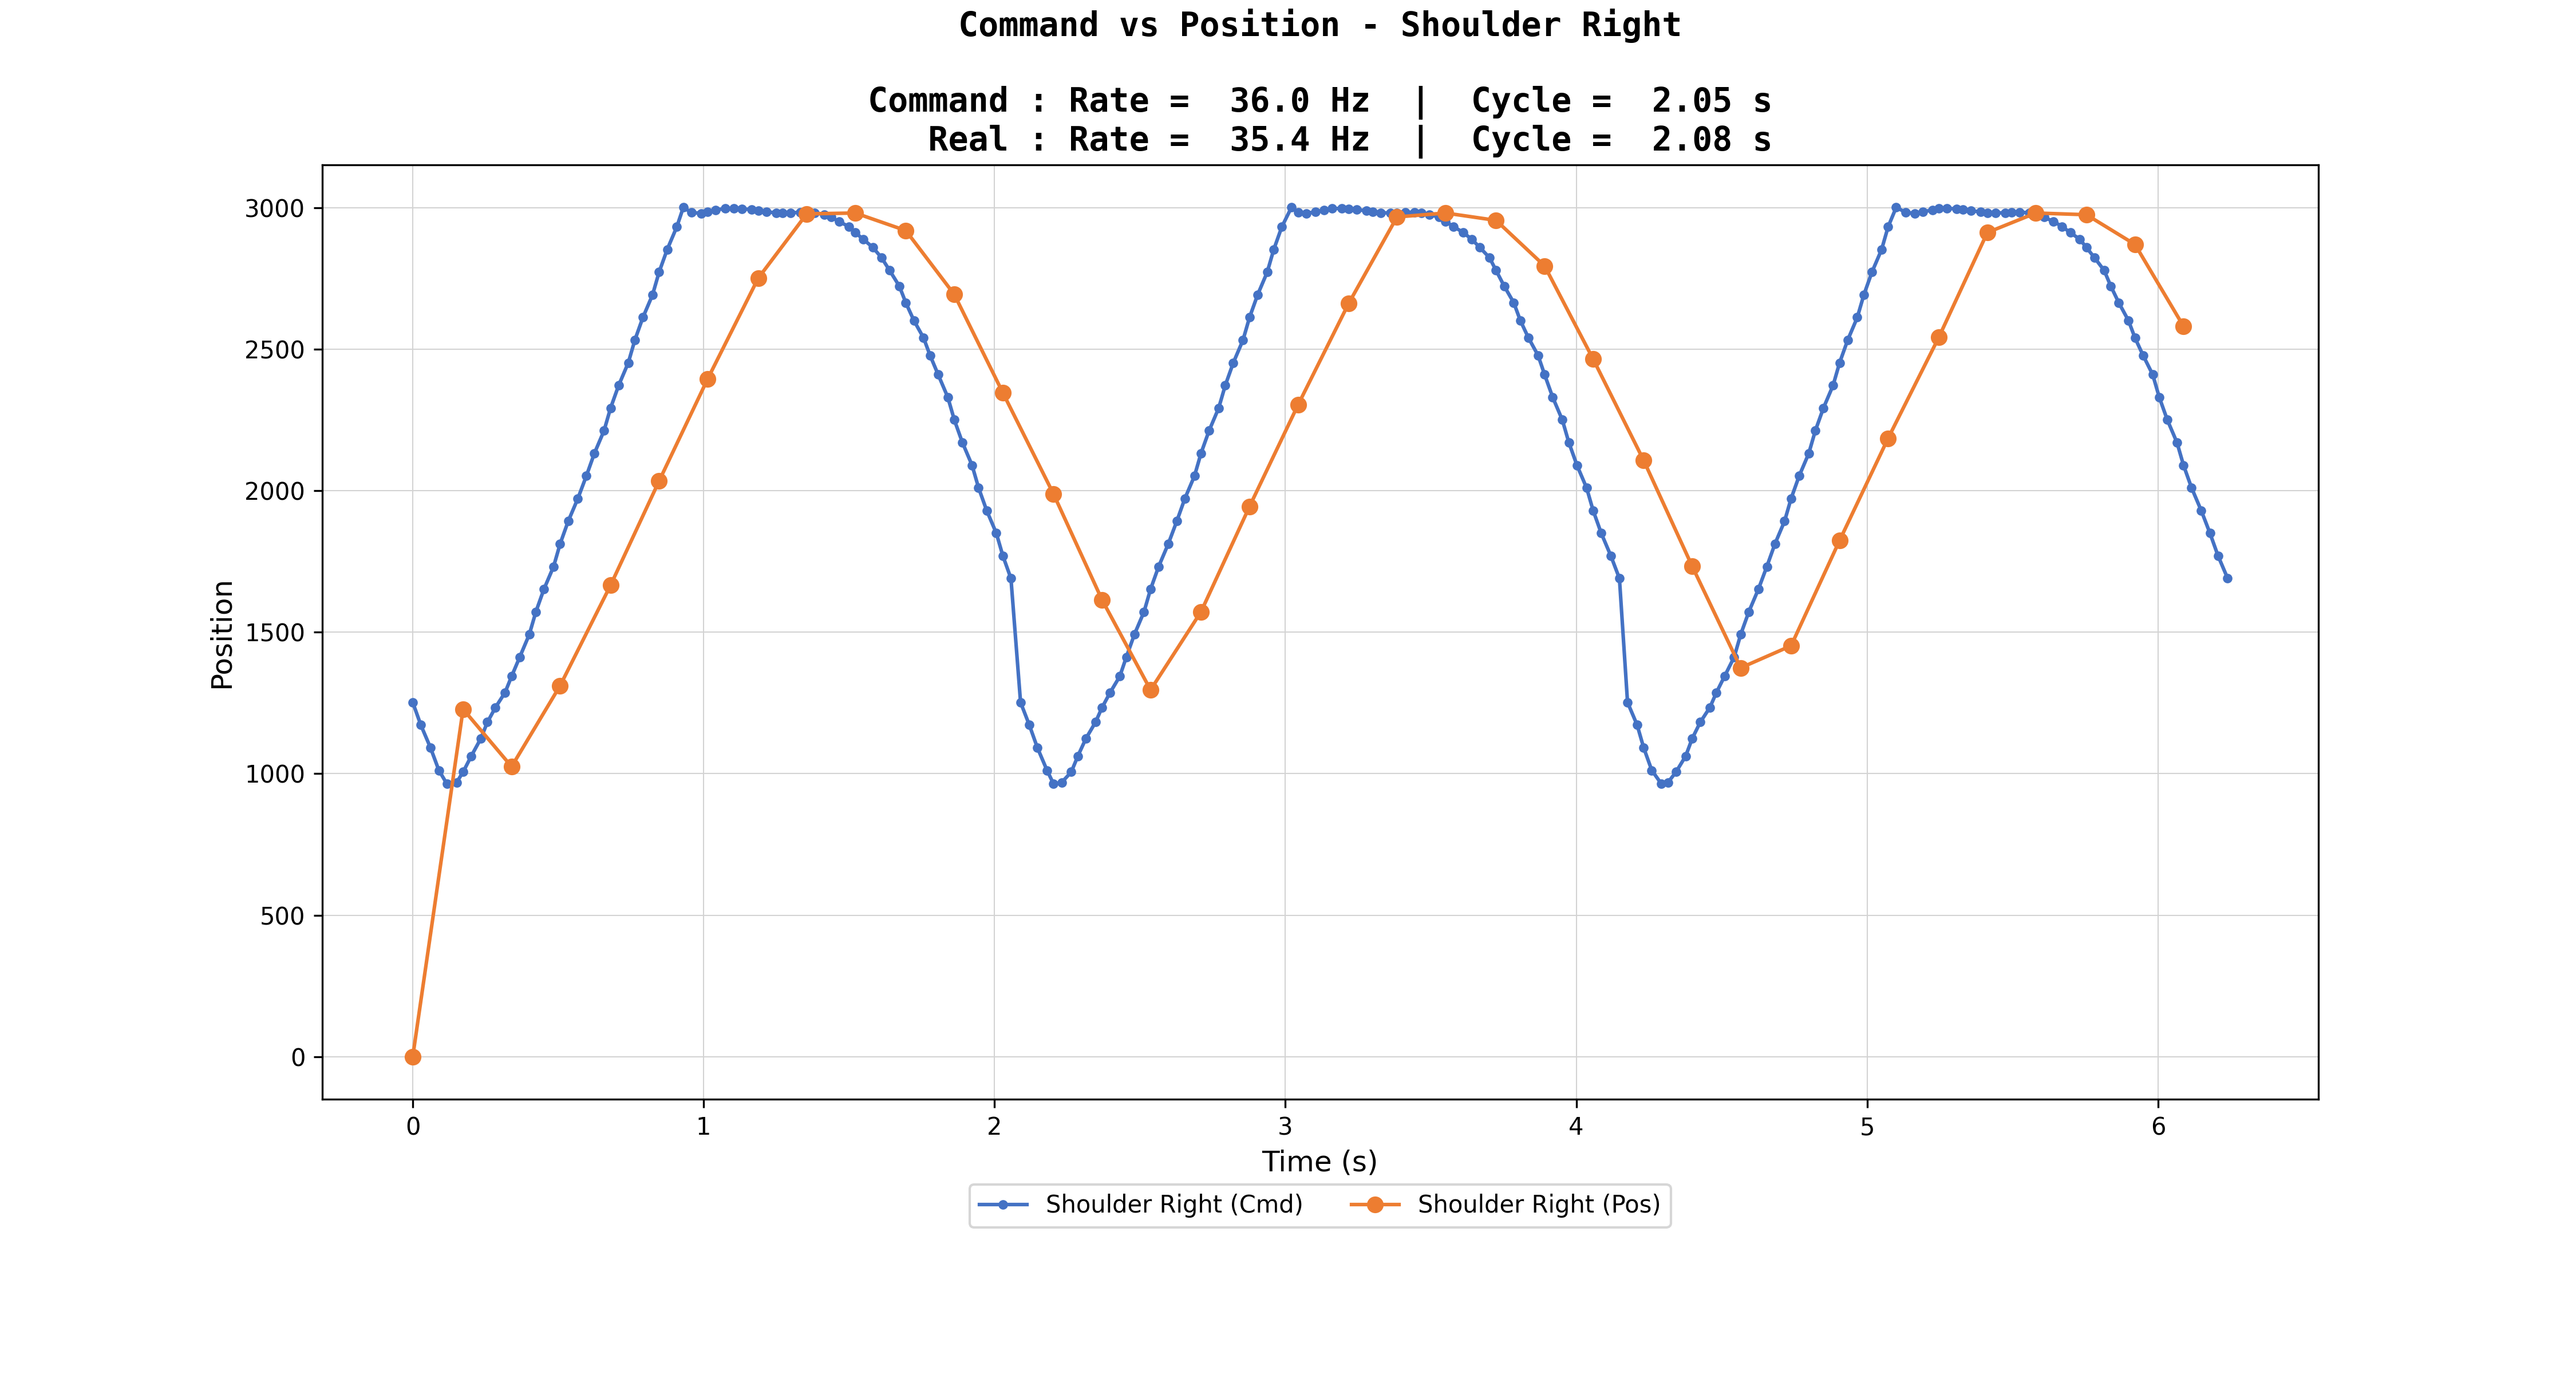
\includegraphics[width=0.8\textwidth]{graphiques/202607141611_ID_4_Spline_Cubic_Pure_36Hz.png}
    \caption{Natural interpolation at 36 Hz.}
    \label{fig:spline_nat_36}
\end{figure}

The problem gets drastically worse at very low frequencies. At 36~Hz, half the nominal frequency, the natural boundary conditions completely distort the motion dynamics at the ends. As Figure~\ref{fig:spline_nat_36} shows, there is an drop in the command at the end of the cycle (at 2.05 s). On the physical robot, this offset translated into a particularly violent mechanical jolt, threatening the integrity of the swim.

To kill this command jump and guarantee a smooth loop, the unknowns $y''_i$ at the nodes must be computed differently. Since the trajectory is meant to be repeated, it is modeled as a \emph{periodic} function of period $N$ : node $x_N$ is identified with node $x_0$ ($y_N \equiv y_0$), and the interpolant $S$ is subjected to the periodic boundary conditions
\begin{equation}
    S(x_0) = S(x_N), \qquad S'(x_0) = S'(x_N), \qquad S''(x_0) = S''(x_N)
    \label{eq:periodiques}
\end{equation}
While positional and acceleration continuities are inherently satisfied by the barycentric form, velocity continuity must be explicitly enforced. Equating the first derivatives of adjacent segments at each node, $S'_{i-1}(x_i) = S'_i(x_i)$, and assuming a uniform step $h=1$ yields the well-known system of N equations :
\begin{equation}
    y''_{i-1} + 4\,y''_i + y''_{i+1} = 6\left(y_{i+1} - 2y_i + y_{i-1}\right)
    \qquad i = 0,\dots,N-1
    \label{eq:systeme-cyclique}
\end{equation}
where all indices are taken modulo $N$. In matrix form, the periodicity introduces two coupling terms at the corners of the matrix, which becomes \emph{cyclic tridiagonal}:
\begin{equation}
    \begin{pmatrix}
        4 & 1 &        &        & 1 \\
        1 & 4 & 1      &        &   \\
          & \ddots & \ddots & \ddots &   \\
          &        & 1      & 4      & 1 \\
        1 &        &        & 1      & 4
    \end{pmatrix}
    \begin{pmatrix} y''_0 \\ y''_1 \\ \vdots \\ y''_{N-2} \\ y''_{N-1} \end{pmatrix}
    =
    6\begin{pmatrix}
        y_1 - 2y_0 + y_{N-1} \\
        y_2 - 2y_1 + y_0 \\
        \vdots \\
        y_{N-1} - 2y_{N-2} + y_{N-3} \\
        y_0 - 2y_{N-1} + y_{N-2}
    \end{pmatrix}
    \label{eq:matrice-cyclique}
\end{equation}

\subsection{Solving the Cyclic System}

%\paragraph{Sherman--Morrison decomposition and the Thomas algorithm:} 

The system~\eqref{eq:matrice-cyclique} is not tridiagonal, but it still solves in $\mathcal{O}(N)$ thanks to the \textsc{Sherman--Morrison} formula~\cite{numerical_recipes}. Let $A$ be the cyclic matrix on the left side of system~\eqref{eq:matrice-cyclique}, this matrix $A$ is, indeed, not strictly tridiagonal because of its two corner coefficients $A_{0,N-1} = A_{N-1,0} = 1$. To avoid a costly full matrix inversion, we write $A$ as a rank-1 perturbation of an ordinary, strictly tridiagonal matrix $T$ according to~\cite{numerical_recipes}:
\begin{equation}
    A = T + u\,v^{\mathsf{T}} \qquad
    u = \begin{pmatrix} \gamma \\ 0 \\ \vdots \\ 0 \\ 1 \end{pmatrix} \qquad
    v = \begin{pmatrix} 1 \\ 0 \\ \vdots \\ 0 \\ 1/\gamma \end{pmatrix}
    \qquad \gamma = -4
    \label{eq:sherman-morrison-setup}
\end{equation}
where $\gamma$ is a free parameter chosen so that $T$ stays well conditioned, here $\gamma = -4$, the opposite of the running diagonal term. The product $u\,v^{\mathsf{T}}$ modifies only the four corners of the matrix:
\begin{equation}
    (u\,v^{\mathsf{T}})_{0,0} = \gamma, \quad
    (u\,v^{\mathsf{T}})_{0,N-1} = \gamma/\gamma = 1, \quad
    (u\,v^{\mathsf{T}})_{N-1,0} = 1, \quad
    (u\,v^{\mathsf{T}})_{N-1,N-1} = 1/\gamma
\end{equation}
so that $T = A - u\,v^{\mathsf{T}}$ is \emph{exactly} tridiagonal, with diagonal
\begin{equation}
    T_{i,i} =
    \begin{cases}
        4 - \gamma = 8 & \text{if } i = 0, \\[2pt]
        4 - \dfrac{1}{\gamma} = 4.25 & \text{if } i = N-1, \\[6pt]
        4 & \text{otherwise,}
    \end{cases}
    \qquad T_{i,i-1} = T_{i,i+1} = 1
    \label{eq:T-diag}
\end{equation}
and sub/super-diagonals all equal to~1 (interior indices). To solve the original system $A\,y'' = d$ without explicitly computing a costly matrix inversion, we apply the \textsc{Sherman--Morrison} formula. This theorem provides the analytical inverse of a matrix that has been modified by a rank-1 update~\cite{numerical_recipes} :
\begin{equation}
    A^{-1} = (T + u\,v^{\mathsf{T}})^{-1} = T^{-1} - \frac{T^{-1} u\,v^{\mathsf{T}} T^{-1}}{1 + v^{\mathsf{T}} T^{-1} u}
\end{equation}

Multiplying both sides by the right-hand vector $d$ yields the solution for $y''$ :
\begin{equation}
    y'' = A^{-1} d = T^{-1} d - \frac{T^{-1} u \left(v^{\mathsf{T}} T^{-1} d\right)}{1 + v^{\mathsf{T}} T^{-1} u}
\end{equation}

To completely avoid the $\mathcal{O}(N^3)$ operation of calculating $T^{-1}$, we define two intermediate vectors $z$ and $w$ such that $z = T^{-1} d$ and $w = T^{-1} u$. Finding these vectors is computationally equivalent to solving two \emph{ordinary}, strictly tridiagonal systems:
\begin{equation}
    T z = d \qquad \text{and} \qquad T w = u
\end{equation}

Substituting $z$ and $w$ back into the analytical solution dramatically simplifies the final equation:
\begin{equation}
    y'' = z - \frac{v^{\mathsf{T}} z}{1 + v^{\mathsf{T}} w}\; w
    \label{eq:sherman-morrison-solution}
\end{equation}

Furthermore, given the sparse form of $v$, the dot product reduces to a simple scalar evaluation $v^{\mathsf{T}} z = z_0 + z_{N-1}/\gamma$ and likewise for $v^{\mathsf{T}} w$. So only the head and tail components of the vectors matter, and no full matrix is ever formed explicitly.

Finally, each of the two tridiagonal systems $T z = d$ and $T w = u$ is solved by the Thomas algorithm (Tridiagonal Matrix Algorithm, TDMA)~\cite{burden_faires}, an optimized variant of Gaussian elimination specialized for tridiagonal matrices, which operates in $\mathcal{O}(N)$ complexity instead of the $\mathcal{O}(N^3)$ required for a general inversion.

Consider a generic system $T x = r$, where $r$ is the right-hand side vector, representing either $d$ or $u$. Since the sub-diagonals and super-diagonals are all equal to~1, the algorithm runs in two passes:

\begin{enumerate}
    \item \textbf{Forward sweep (elimination):} We eliminate the sub-diagonal terms row by row. For the very first row ($i=0$), the equation is simply $T_{0,0}\, x_0 + x_1 = r_0$. Dividing by the pivot $T_{0,0}$ isolates $x_0$ and defines our initial modified coefficients:
    \begin{equation}
        c'_0 = \frac{1}{T_{0,0}}, \qquad x_0 = \frac{r_0}{T_{0,0}}
    \end{equation}
    Then, for $i = 1, \dots, N-1$, we substitute the previous row into the current one. Noting that the effective pivot of row $i$ after eliminating column $i-1$ becomes $m_i = T_{i,i} - c'_{i-1}$, we update the coefficients :
    \begin{equation}
        m_i = T_{i,i} - c'_{i-1}, \qquad
        c'_i = \frac{1}{m_i}, \qquad
        x_i = \frac{r_i - x_{i-1}}{m_i}
        \label{eq:thomas-forward}
    \end{equation}
    At the end of this pass, the system has been reduced to an equivalent \emph{upper bidiagonal} form.
    
    \item \textbf{Back substitution:} We walk the indices in reverse to propagate the corrections left pending by the super-diagonal terms ($c'_i$) during the forward sweep:
    \begin{equation}
        x_i \leftarrow x_i - c'_i\, x_{i+1}, \qquad i = N-2,\, N-3,\, \dots,\, 0
        \label{eq:thomas-backward}
    \end{equation}
\end{enumerate}

Each of the two passes costs only $\mathcal{O}(N)$ arithmetic operations, and the matrix $T$ is factorized only once. So the total compute cost therefore stays linear in $N$, which allows the instant recomputation of the high-frequency trajectory for all 21 joints whenever a parameter is adjusted on the interface.

Once the vector $y''$ is known, the closed curve is evaluated at $F$ points evenly spread over one period, \emph{excluding} the joining point which belongs to the next cycle :
\begin{equation}
    x_k = k\,\frac{N}{F}, \qquad k = 0,\, 1,\, \dots,\, F-1
\end{equation}
so that the number of frames produced respects exactly $F = f_{\mathrm{Hz}} \times T_{\mathrm{cycle}}$ and the next frame ($k = F$, first frame of the next cycle) falls precisely on $S(x_N) = y_0$.

This new formulation solves the discontinuity problem at the source. Taking again the critical case of subsampling at 36~Hz, as we can observe from Figure~\ref{fig:spline_per_36} demonstrates the method's success perfectly :

\begin{figure}[H]
    \centering
    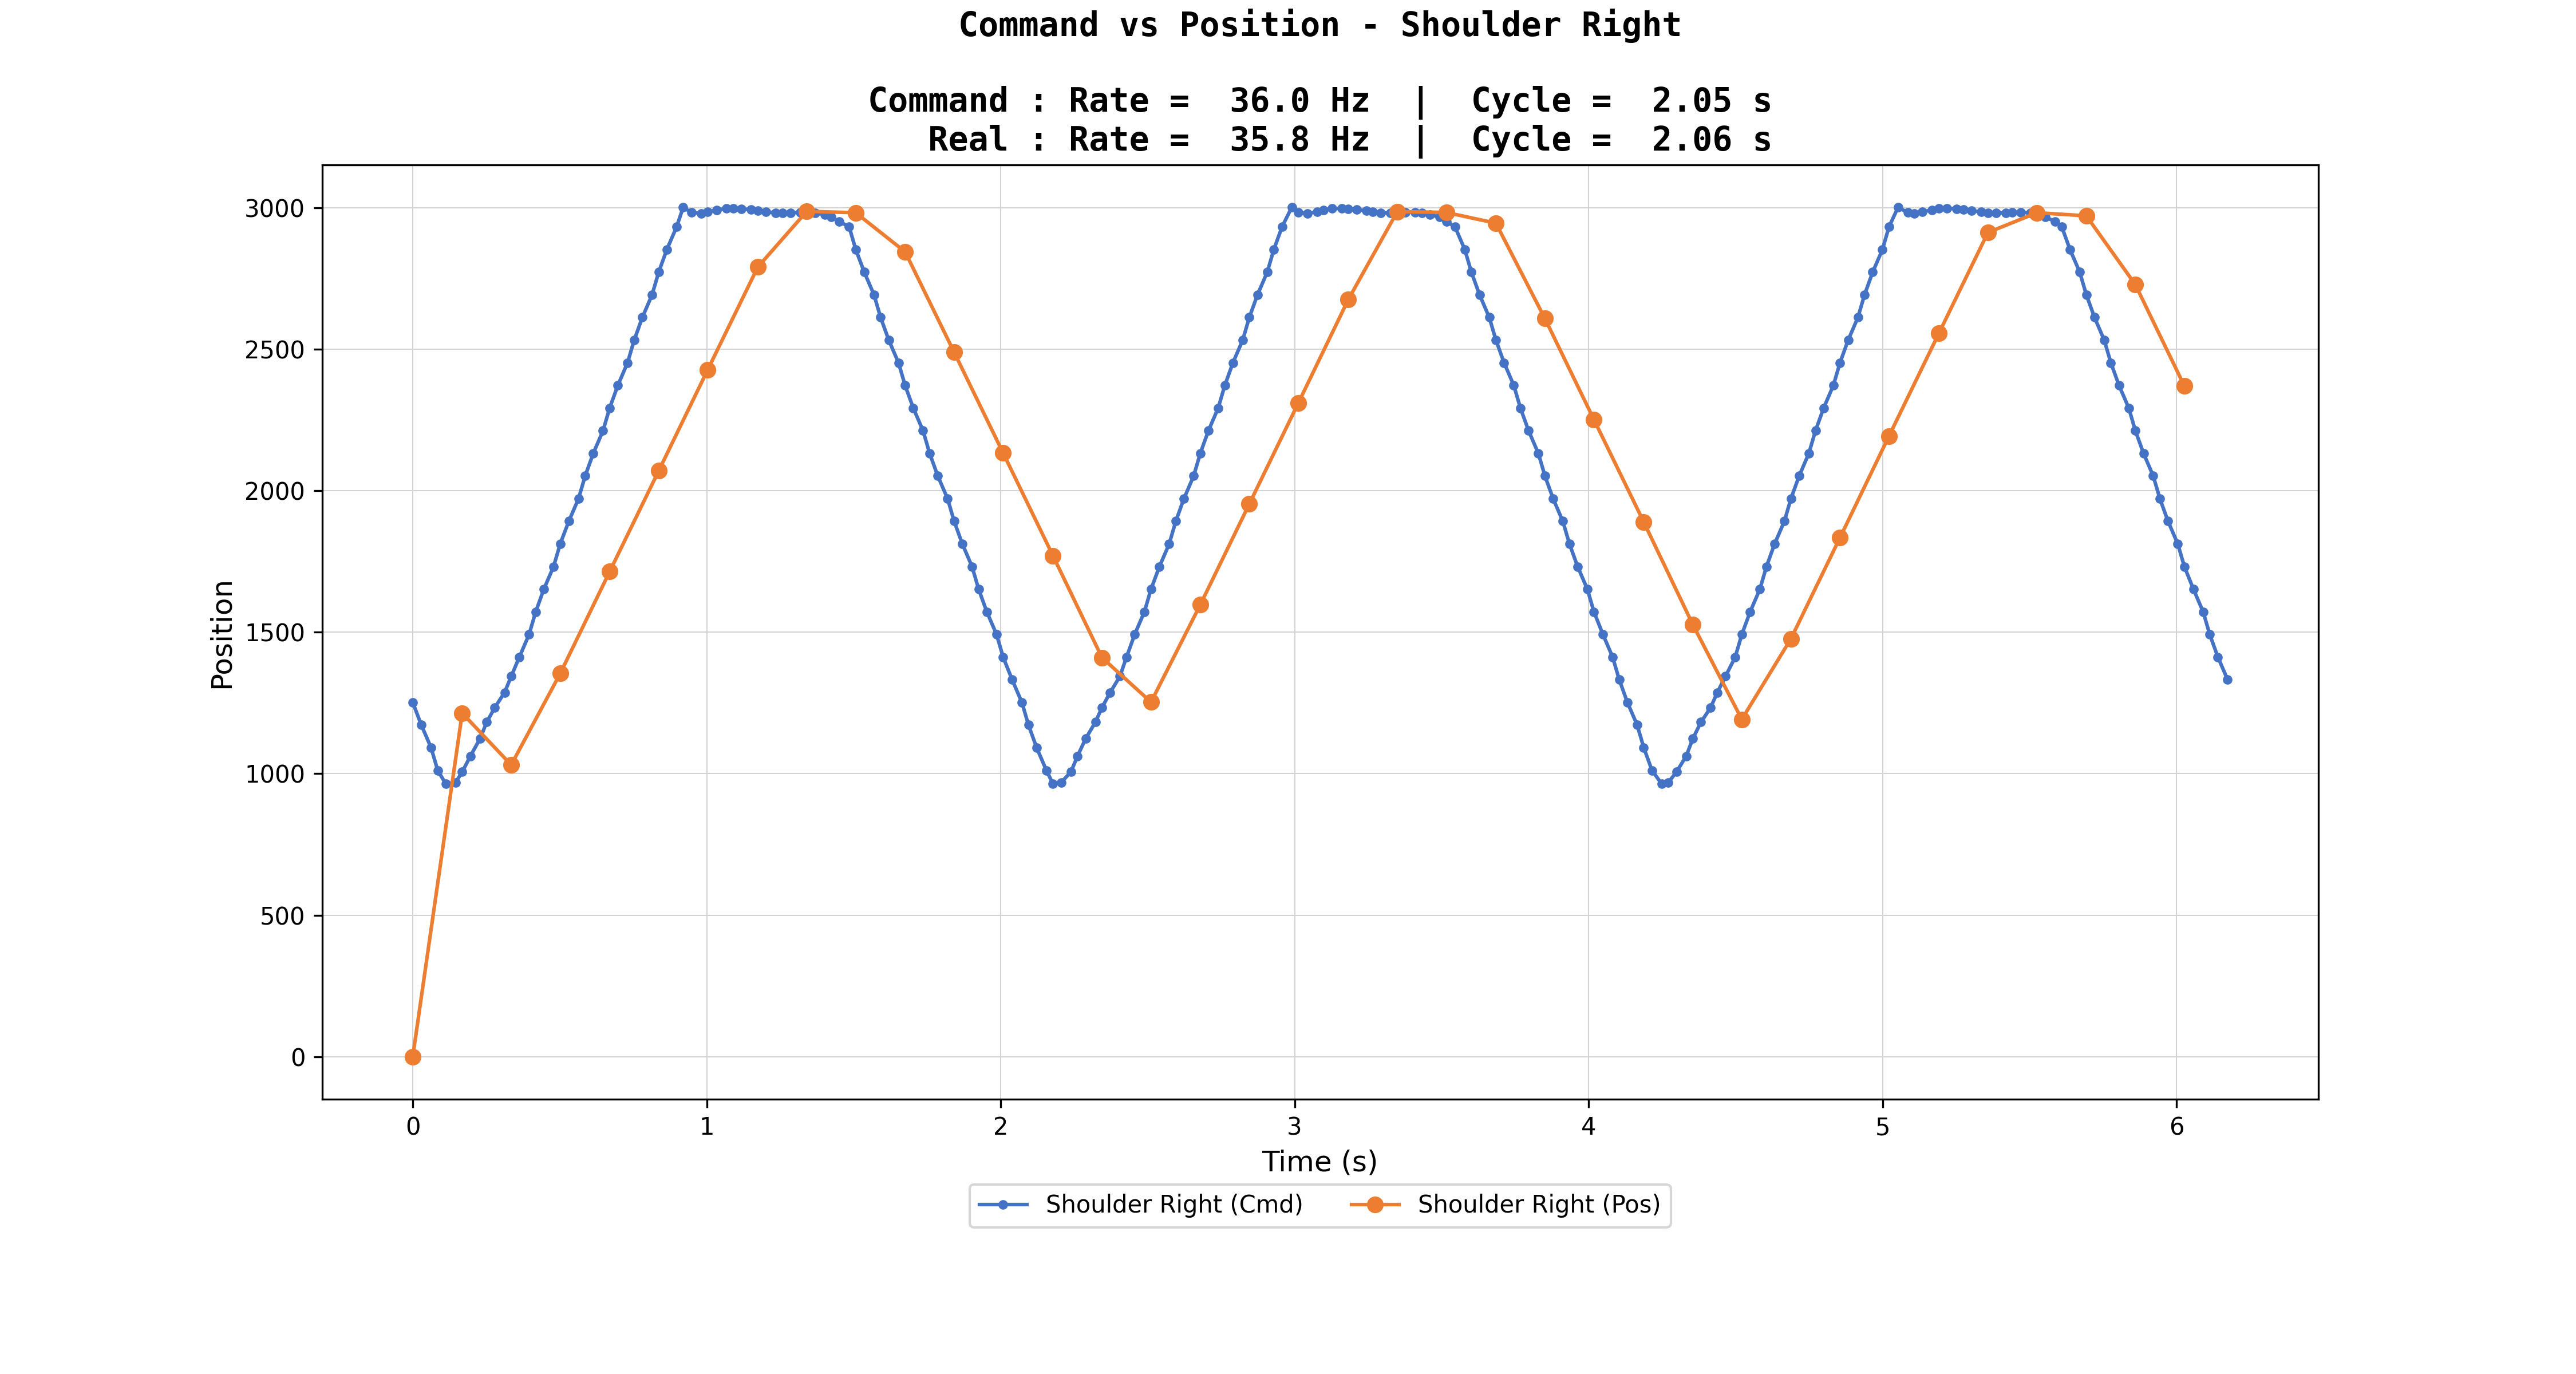
\includegraphics[width=0.8\textwidth]{graphiques/202607141717_ID_4_Spline_Cubique_Periodique_36Hz.png}
    \caption{Periodic interpolation at 36 Hz.}
    \label{fig:spline_per_36}
\end{figure}

In the graph we see the command curve, in blue, which anticipates the end of the cycle and joins the start of the next one perfectly smoothly. The transition, after 2 seconds, happens with no break in slope, definitively eliminating the mechanical jolts.

This structural continuity holds naturally at intermediate frequencies. The figure~\ref{fig:spline_per_50} shows that at 50~Hz, where the natural spline had a visible drop, the periodic spline gives a flawless closed loop. The signal chains together seamlessly over infinite cycles.

\begin{figure}[H]
    \centering
    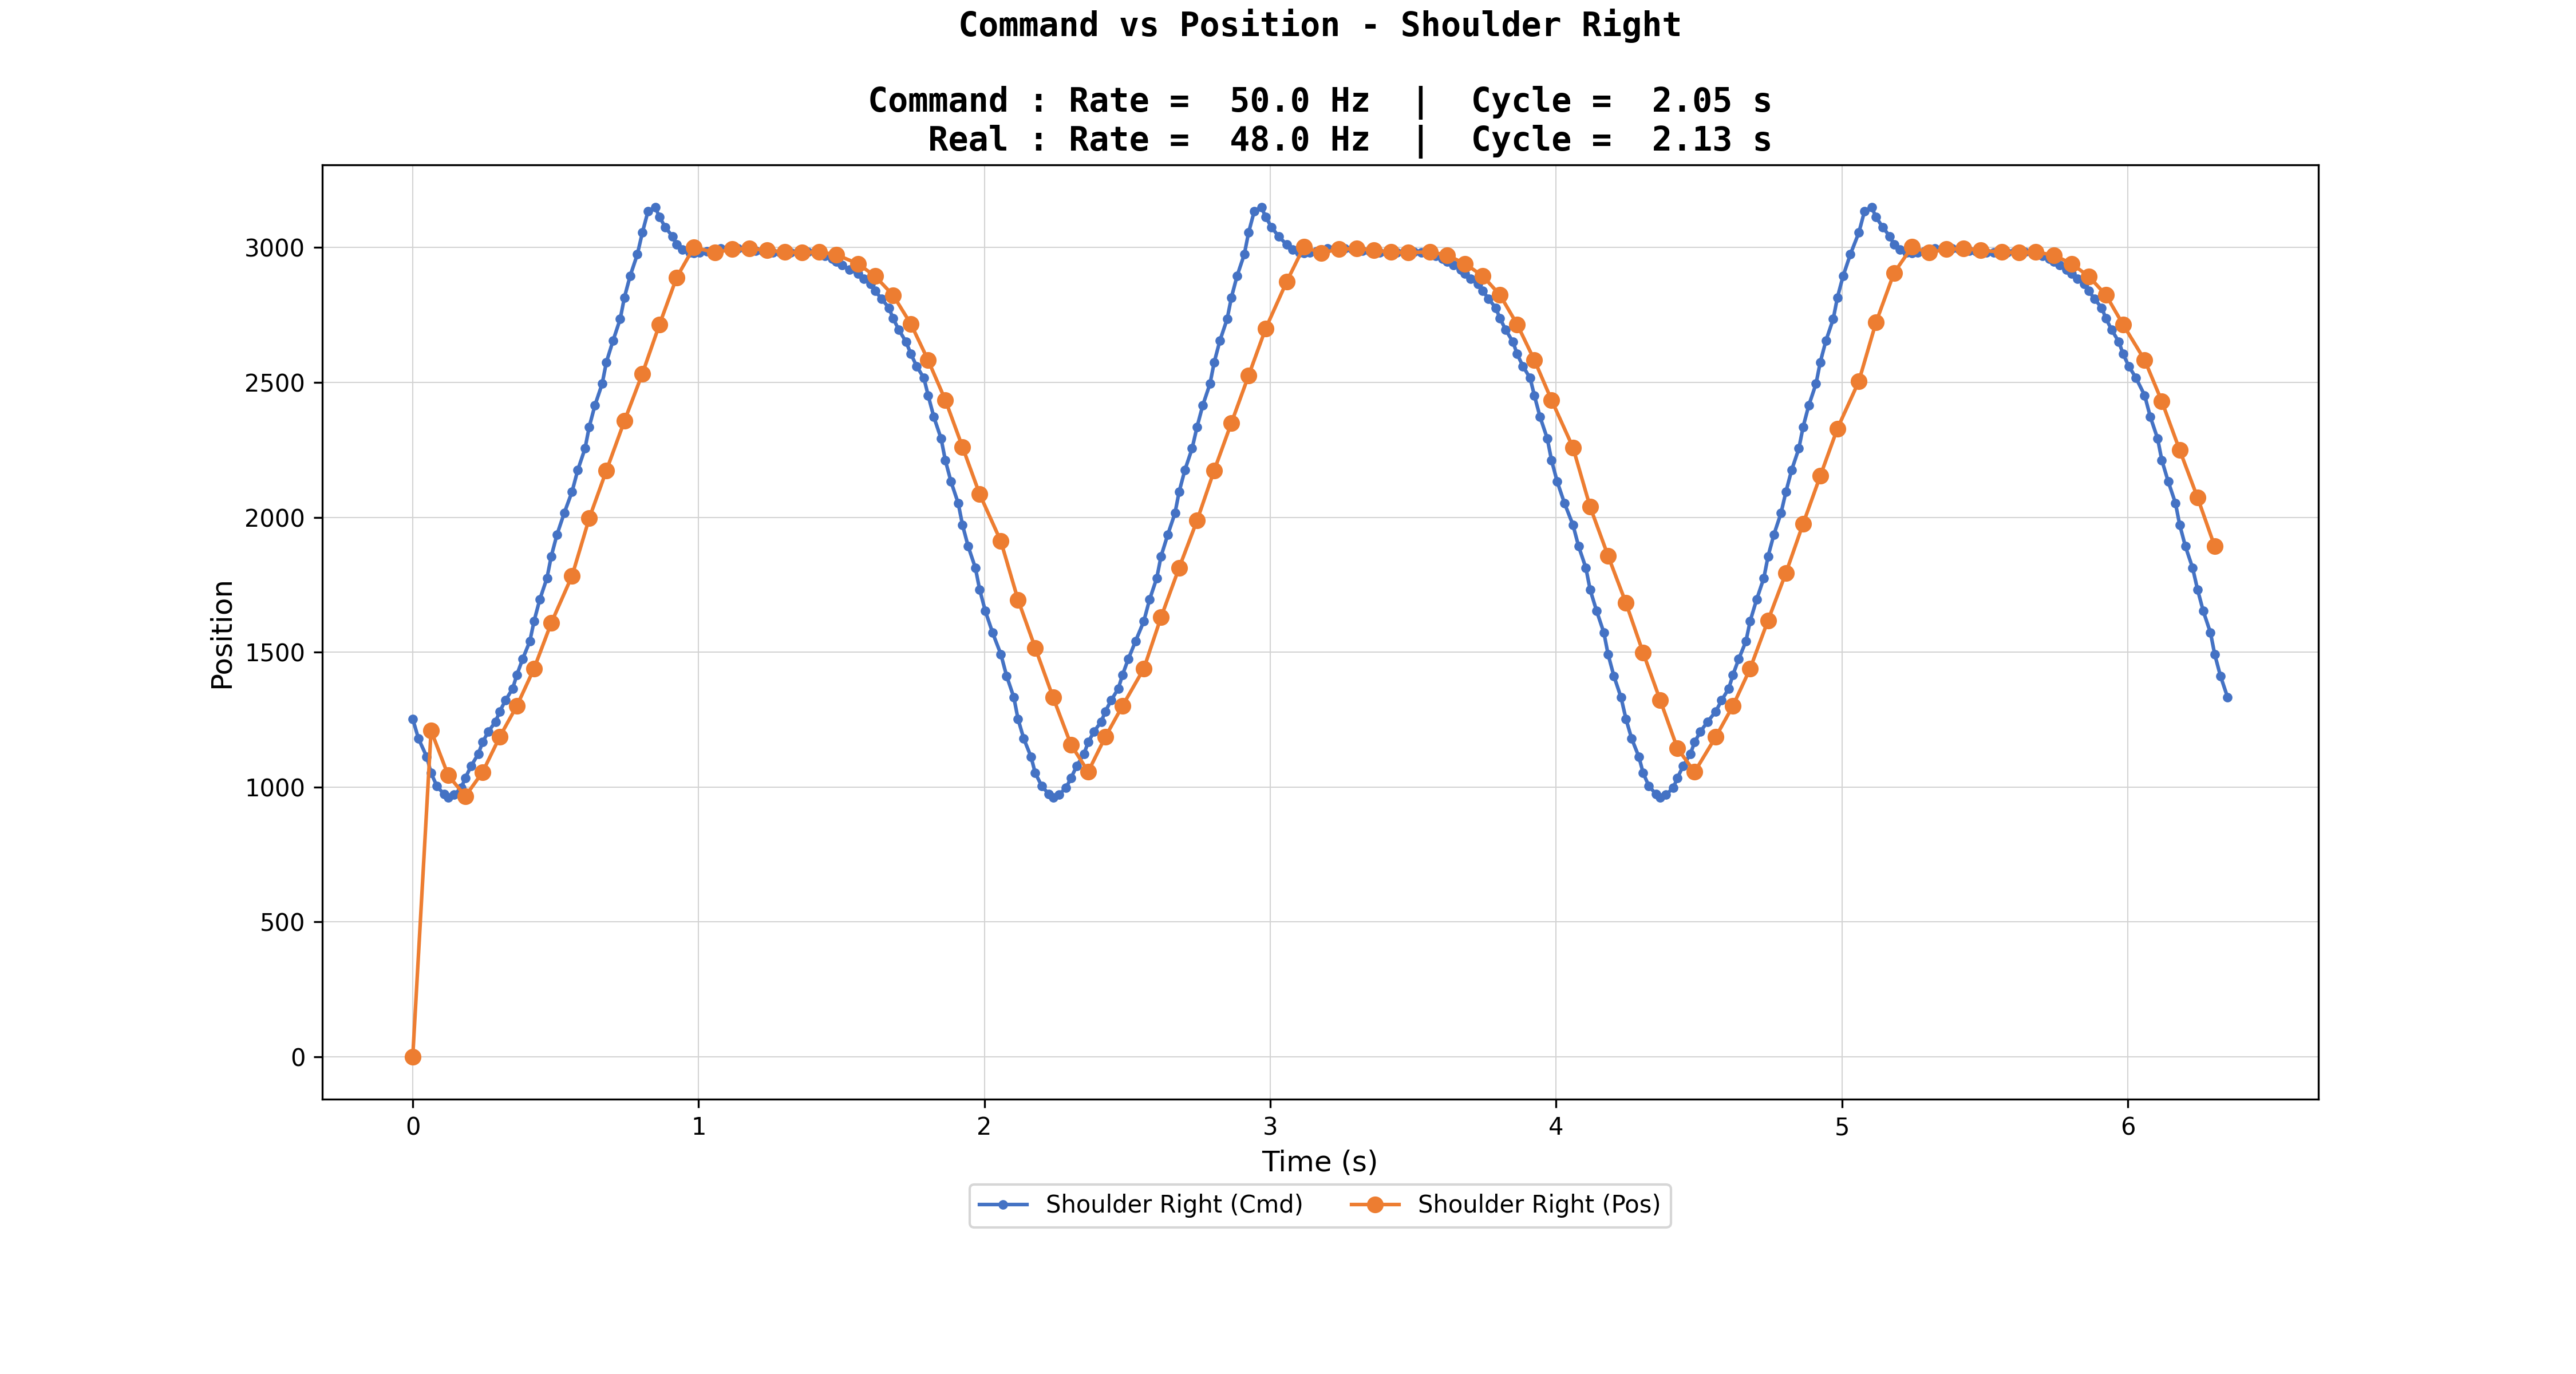
\includegraphics[width=0.8\textwidth]{graphiques/202607141720_ID_4_Spline_Cubique_50Hz.png}
    \caption{Periodic interpolation at 50 Hz.}
    \label{fig:spline_per_50}
\end{figure}

Finally, at high frequency (90~Hz), the method keeps the very high fidelity of the motion while guaranteeing a perfect join at the ends, as the figure~\ref{fig:spline_per_90} shows below. So the periodic spline is therefore the best choice for the SWUMANOID's motion interpolation, as it guarantees a smooth trajectory at any control frequency.

\begin{figure}[H]
    \centering
    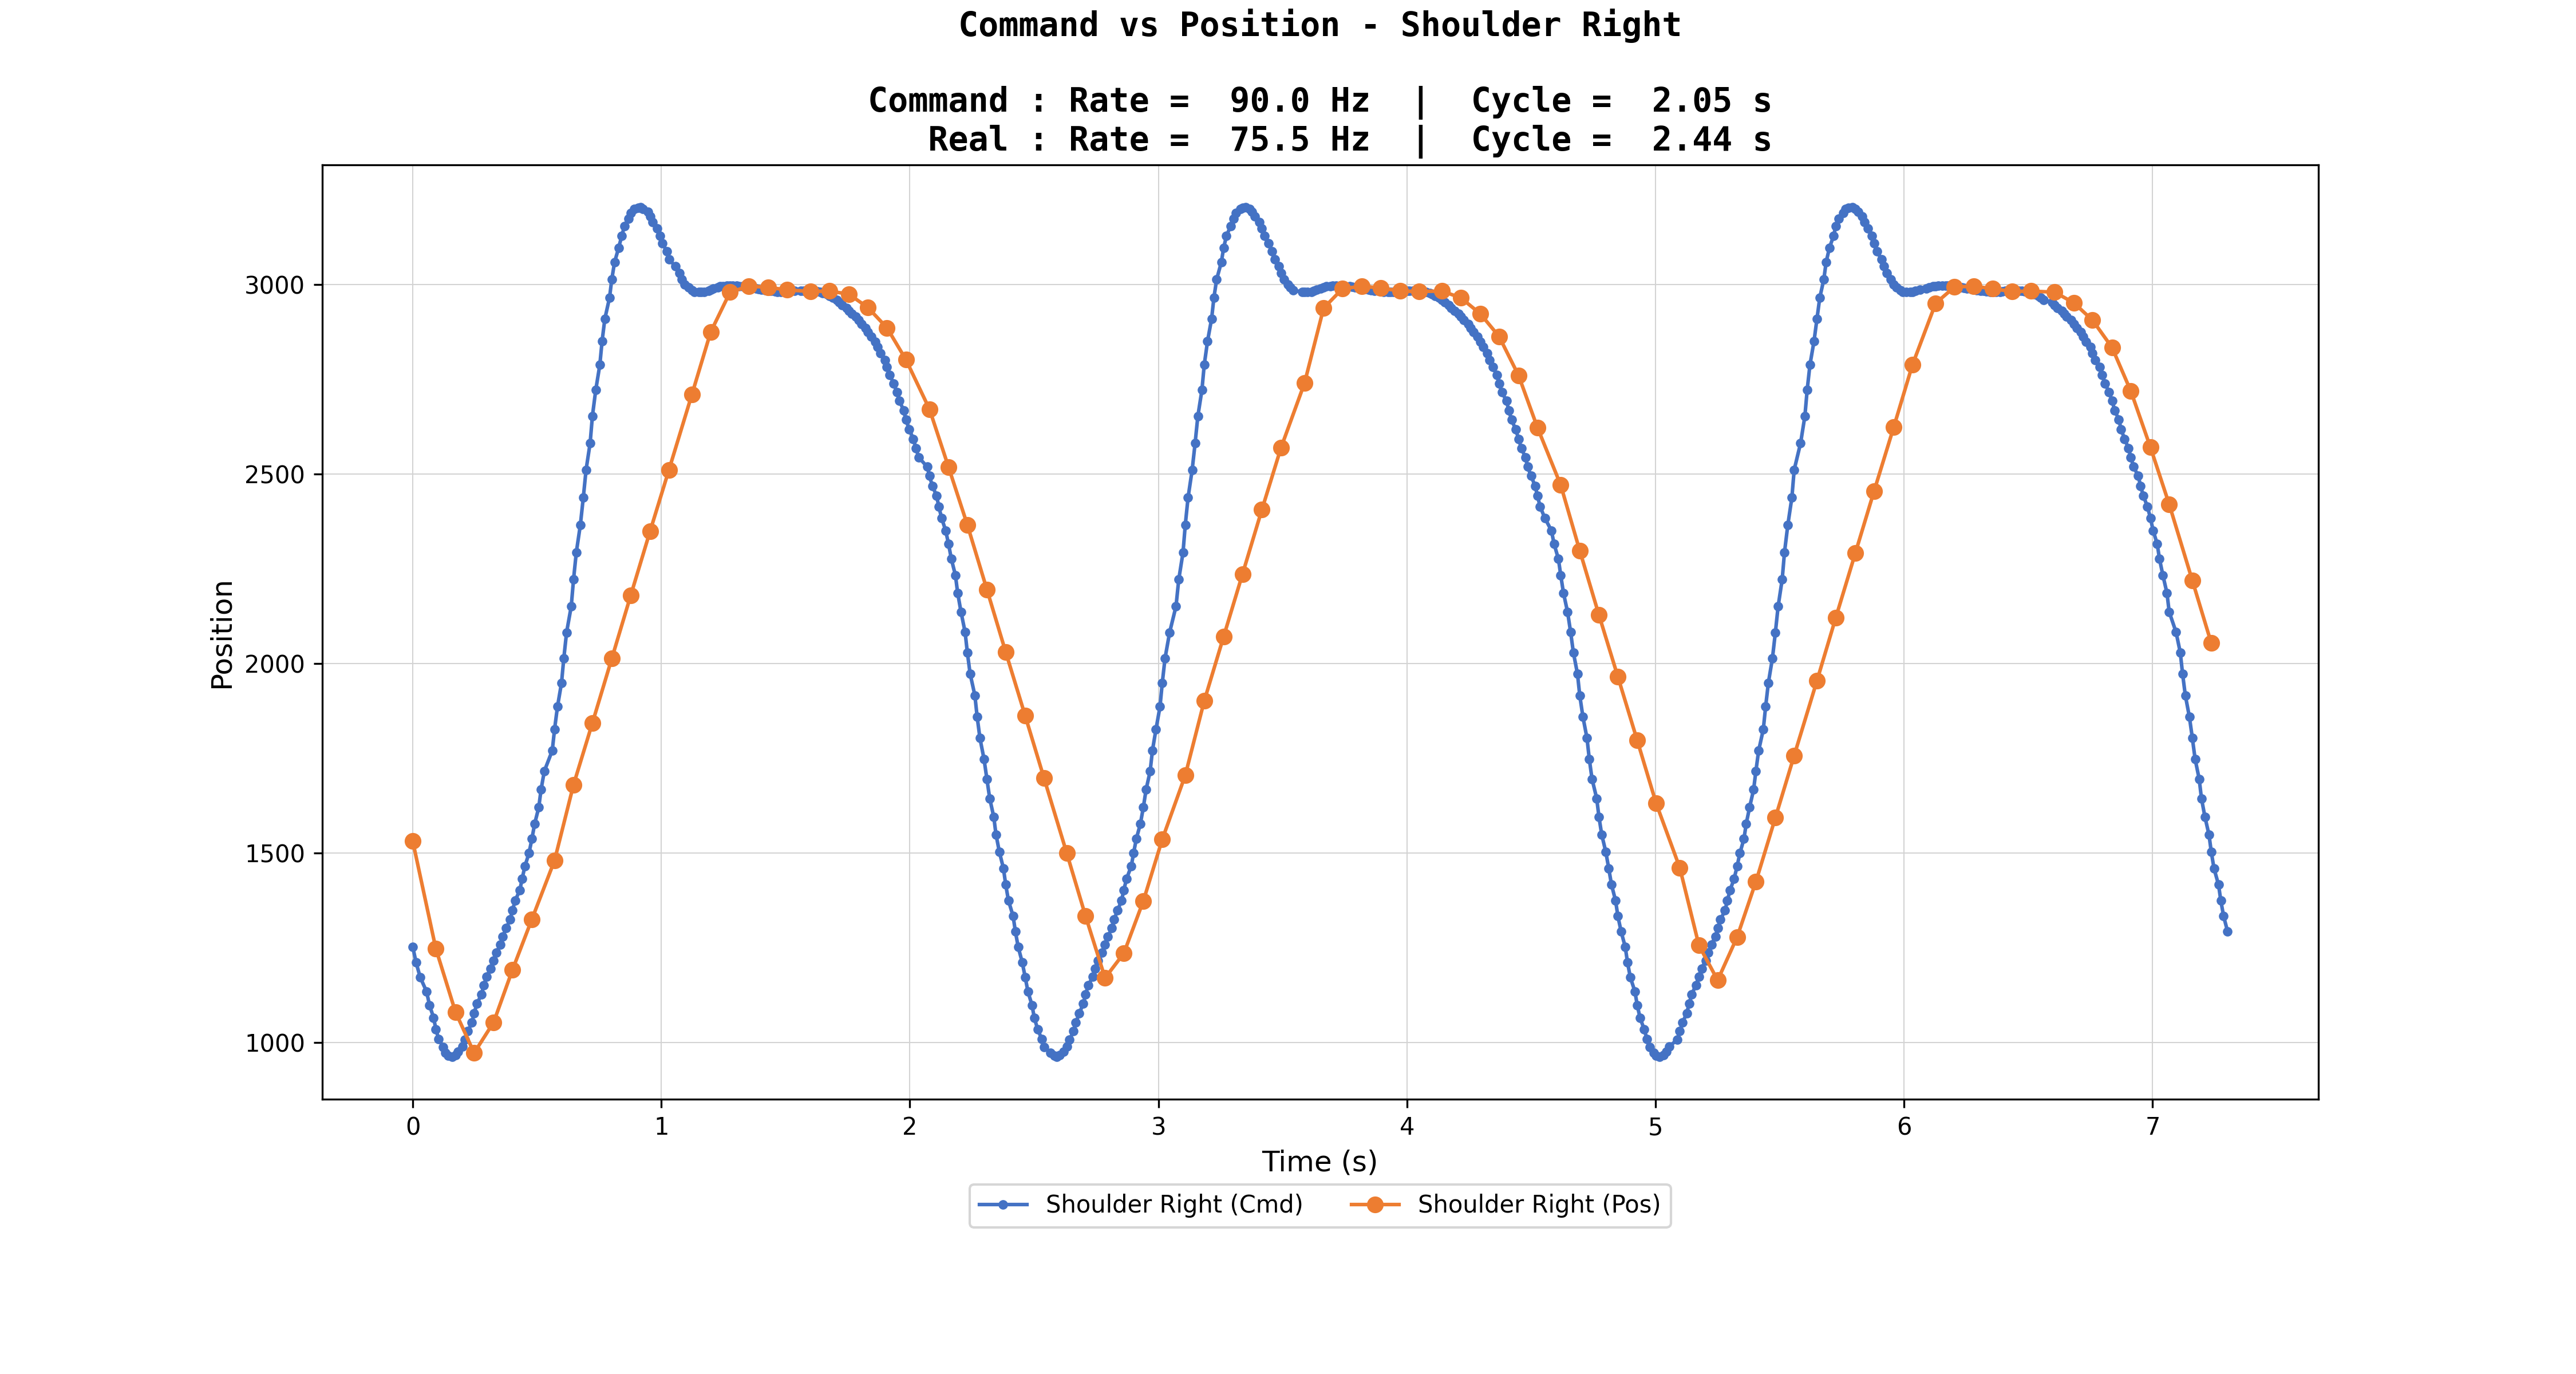
\includegraphics[width=0.8\textwidth]{graphiques/202607141725_ID_4_Spline_Cubique_Periodique_90Hz.png}
    \caption{Periodic interpolation at 90 Hz.}
    \label{fig:spline_per_90}
\end{figure}

By construction of the periodic interpolant~\eqref{eq:periodiques}, position, velocity and acceleration are continuous at the loop-back so the join between two consecutive cycles is class $\mathcal{C}^2$, just like any interior point of the trajectory. The momentum of the swimming stroke is thus fully preserved from one cycle to the next, and the motor jolts at loop-back are eliminated not approximately but exactly. In practice, the residual velocity discontinuity measured at the join is smaller than the maximum velocity variation observed inside the cycle. Moreover if the source file ends explicitly with a copy of its first frame, this duplicate is removed before fitting so as not to introduce a double node in the period.


\subsection{Minimum-Jerk Ramp}

For the move to the initial pose, the C++ firmware now generates a degree-5 polynomial approach trajectory (\textit{minimum-jerk}). The normalized time equation is:
\begin{equation}
s(t) = 6t^5 - 15t^4 + 10t^3, \quad t \in [0,1]
\end{equation}
The joint command at instant $k$ is then computed smoothly by:
\begin{equation}
q_k = q_{start} + s\left(\frac{k}{g_{rampSteps}}\right) \cdot (q_{goal} - q_{start})
\end{equation}
This software safeguard is paired with a temporary hardware speed limit via the Dynamixel registers, as shown in Table \ref{tab:hardware_profile}.

\begin{table}[h]
\centering
\begin{tabular}{|l|c|l|}
\hline
\textbf{Register} & \textbf{Address} & \textbf{Value at initialization} \\ \hline
\texttt{Profile Acceleration} & 108 & \texttt{10} (very gentle acceleration) \\ \hline
\texttt{Profile Velocity} & 112 & \texttt{40} ($\approx 9$ rpm) \\ \hline
\end{tabular}
\caption{Hardware speed limiting of the actuators.}
\label{tab:hardware_profile}
\end{table}

To \textbf{fix the CPU loop}, the 15 Hz limitation was resolved by drastically separating the blocking UART calls from the network handling (SSE), and by forcing a reset of the ESP32's hardware timers when the motion starts.

% \section{Implementing a PID controller}



\section{Angular Configuration of the SWUMANOID via the IMU}
\label{sec:calcul_angle}

This section formalizes, in full, the kinematic processing chain chosen to estimate the \emph{roll} ($\phi$, around the longitudinal axis $X$) and \emph{yaw} ($\psi$, around the vertical $Z$) angles of the SWUMANOID robot from the inertial unit (IMU) housed in the AtomS3R. The unit provides only a three-axis accelerometer $\mathbf{a}=(A_x,A_y,A_z)^{\mathsf T}$ and a three-axis gyroscope $\boldsymbol{\omega}=(G_x,G_y,G_z)^{\mathsf T}$, expressed in the AtomS3R's \emph{board} frame $\mathcal{B}$ neither an attitude quaternion nor a magnetometer is transmitted.

The attitude is therefore reconstructed entirely on the client, transformed into the robot frame $\mathcal{R}$, referenced by a tare operation, then smoothed. The adopted convention is \emph{Z-Up} (the robot's vertical axis pointing up), in line with robotics standards.

\begin{figure}[H]
    \centering
    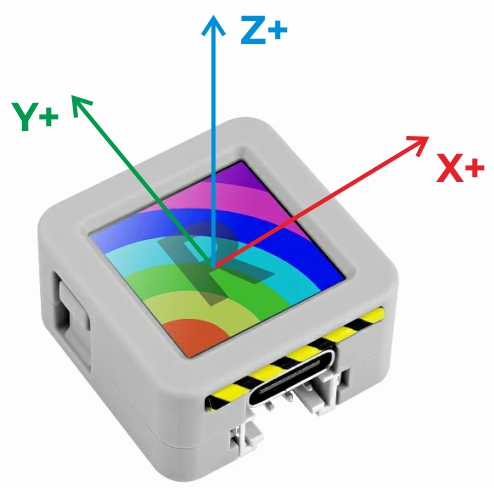
\includegraphics[width=0.25\linewidth]{schemas/IMU-AtomS3R_Defaut_Axes.png}
    \caption{Axis orientation of the AtomS3R base.}
    \label{fig:imu_axes}
\end{figure}

We write unit quaternions as $q=(q_w,q_x,q_y,q_z)$ (scalar part first), $\otimes$ for the Hamilton product, $q^{*}$ for the conjugate and, for a unit quaternion, $q^{-1}=q^{*}$. The world frame $\mathcal{W}$ is aligned with gravity, $\mathbf{z}_{\mathcal{W}}=(0,0,1)^{\mathsf T}$ pointing up. The AtomS3R's default axes and the SWUMANOID's target frame are shown respectively in the figure~\ref{fig:imu_axes} and~\ref{fig:swumanoid_frame}.


\begin{figure}[H]
    \centering
    \begin{subfigure}[b]{\textwidth}
        \centering
        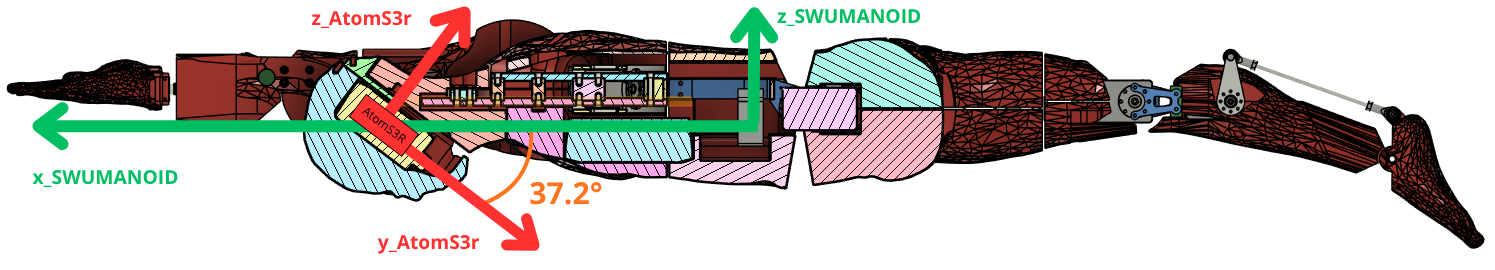
\includegraphics[width=0.8\linewidth]{schemas/AtomS3R_SWUMANOID_orientation_side_view.png}
        \caption{Side view of the SWUMANOID.}
    \end{subfigure}

    \vspace{0.4cm}

    \begin{subfigure}[b]{\textwidth}
        \centering
        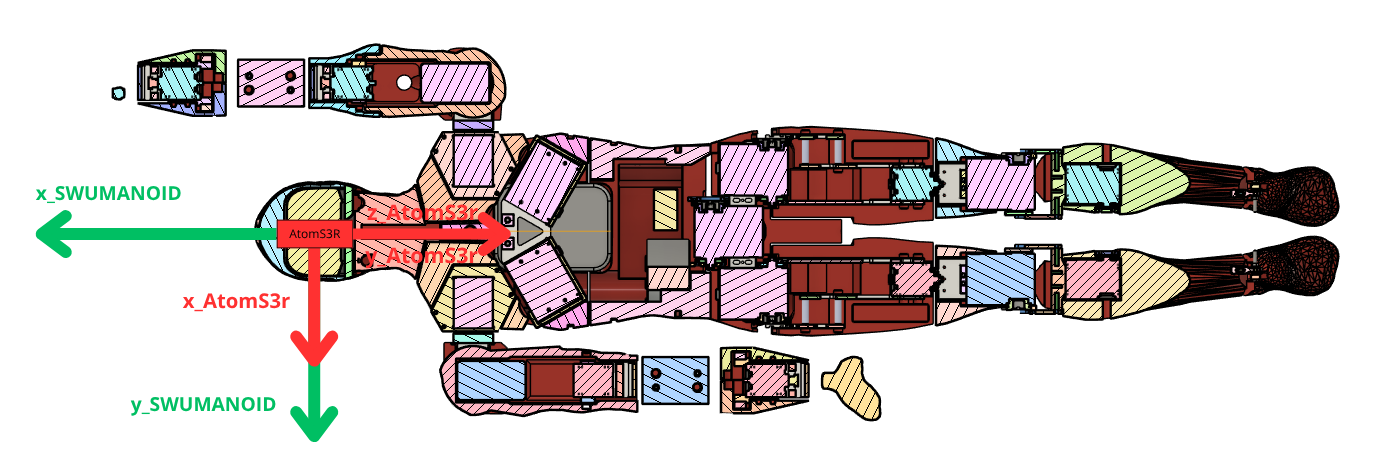
\includegraphics[width=0.8\linewidth]{schemas/AtomS3R_SWUMANOID_orientation_Back_View.png}
        \caption{Back view of the SWUMANOID.}
    \end{subfigure}
    \caption{Global view of the AtomS3R frame axes relative to the robot's target frame.}
    \label{fig:swumanoid_frame}
\end{figure}

\subsection{Acquisition and Fusion of the Raw Data}
\label{subsec:acquisition}

The firmware transmits acceleration in milli-$g$ and angular velocity in deci-degrees per second so the physical quantities are recovered by
\begin{equation}
\mathbf{a}=\frac{1}{1000}\,\mathbf{a}_{\text{raw}}\ [\,g\,],
\qquad
\boldsymbol{\omega}=\frac{1}{10}\,\boldsymbol{\omega}_{\text{raw}}\ [\,^\circ\!/\mathrm{s}\,]
\end{equation}
A dead zone is then applied component by component to the gyroscope, to neutralize the rest noise responsible for the slow yaw drift:
\begin{equation}
\tilde{\omega}_i=
\begin{cases}
0 & \text{if } |\omega_i|<\omega_{\mathrm{db}},\\
\omega_i & \text{otherwise,}
\end{cases}
\qquad i\in\{x,y,z\},\quad \omega_{\mathrm{db}}=1{.}2~^\circ\!/\mathrm{s}
\end{equation}

At rest, the accelerometer measures the reaction to gravity, a vector of unit norm (in $g$) collinear with the local vertical, its projection on the frame axes gives a \emph{drift-free} estimate of the tilt. Assuming a quasi-static sensor, the measured gravity is written in $\mathcal B$ as
\begin{equation}
\mathbf{a}=\mathbf{R}(\phi,\theta)^{\mathsf T}
\begin{pmatrix}0\\0\\1\end{pmatrix}
\end{equation}
which, expanding the rotation matrix for a roll $\phi$ (around $X$) and a pitch $\theta$ (around $Y$), leads to the components
\begin{equation}
A_x=-\sin\theta,\qquad
A_y=\cos\theta\,\sin\phi,\qquad
A_z=\cos\theta\,\cos\phi
\end{equation}
From this, by elimination and using the $\operatorname{arctan2}$ function, which resolves the quadrant ambiguity over $[-\pi,\pi]$, we get the \emph{instantaneous} tilt angles:
\begin{empheq}[box=\fbox]{align}
\phi_{\text{acc}} &= \operatorname{arctan2}\!\big(A_y,\;A_z\big) \label{eq:roll_acc}\\
\theta_{\text{acc}} &= \operatorname{arctan2}\!\Big(-A_x,\;\sqrt{A_y^{2}+A_z^{2}}\Big) \label{eq:pitch_acc}
\end{empheq}
Equation~\eqref{eq:roll_acc} is the physical basis of the roll estimate but the accelerometer has limits. Indeed, it is \emph{blind to yaw}, the gravity is invariant under rotation about the vertical, so $\psi$ appears in none of the equations above, and it is heavily noisy as soon as the sensor undergoes its own acceleration (vibrations from the 21 Dynamixel motors, shocks), the measured vector then no longer being purely gravitational.

The gyroscope provides the instantaneous angular velocity and allows, through integration, a fine and low-latency tracking of orientation, it suffers, on the other hand, from a cumulative drift, an integrated bias. The fusion approach therefore combines the long-term stability of the accelerometer~\eqref{eq:roll_acc}--\eqref{eq:pitch_acc} with the short-term reactivity of the gyroscope. Rather than manipulate Euler angles (prone to gimbal lock), the orientation is carried by an attitude quaternion $q_{\text{raw}}$ ($\mathcal B\rightarrow\mathcal W$) whose kinematics obey this equation :
\begin{equation}
\dot{q}=\tfrac{1}{2}\,q\otimes
\begin{pmatrix}0\\ \boldsymbol{\omega}\end{pmatrix}
\label{eq:kinematics}
\end{equation}
with $\boldsymbol{\omega}$ expressed in the body frame. The implementation integrates~\eqref{eq:kinematics} with the exact exponential map on each interval $\Delta t$ measured locally, it means setting $\boldsymbol{\omega}$ in $\mathrm{rad/s}$, $\Omega=\lVert\boldsymbol{\omega}\rVert$ and $\mathbf{n}=\boldsymbol{\omega}/\Omega$,
\begin{equation}
\delta q=\Big(\cos\tfrac{\Omega\,\Delta t}{2},\;\mathbf{n}\,\sin\tfrac{\Omega\,\Delta t}{2}\Big),
\qquad
q_{\text{raw}}\leftarrow q_{\text{raw}}\otimes\delta q
\label{eq:gyro_step}
\end{equation}
The post-multiplication on the right, reflects the \emph{local} nature of the rotation measured by the gyroscope.

Let $\hat{\mathbf{u}}=\mathbf{a}/\lVert\mathbf{a}\rVert$ be the direction of gravity measured in $\mathcal B$. The initial quaternion is the shortest arc bringing $\hat{\mathbf{u}}$ onto $\mathbf{z}_{\mathcal W}$:
\begin{equation}
q_{\text{raw}}^{(0)}=\frac{\big(1+\hat{\mathbf{u}}\cdot\mathbf{z}_{\mathcal W},\;\hat{\mathbf{u}}\times\mathbf{z}_{\mathcal W}\big)}{\big\lVert\big(1+\hat{\mathbf{u}}\cdot\mathbf{z}_{\mathcal W},\;\hat{\mathbf{u}}\times\mathbf{z}_{\mathcal W}\big)\big\rVert}
\label{eq:seed}
\end{equation}
so that the estimate starts flat, with the yaw arbitrarily fixed to zero, a purely relative heading.

At each sample, the gyroscope prediction~\eqref{eq:gyro_step} is realigned on gravity \emph{only when} the measurement is judged quasi-static, that is $\big|\,\lVert\mathbf{a}\rVert-1\,\big|\le\tau$ with $\tau=0{.}25\,g$, this test discards the self-acceleration phases, where gravity is masked. The predicted vertical in the body frame is
\begin{equation}
\hat{\mathbf{g}}_{\text{pred}}=q_{\text{raw}}^{-1}\otimes\mathbf{z}_{\mathcal W}\otimes q_{\text{raw}}
\end{equation}
and we build the correction quaternion $\delta q_c$ realizing the shortest arc from the \emph{measured} vertical $\hat{\mathbf{u}}$ to the \emph{predicted} vertical $\hat{\mathbf{g}}_{\text{pred}}$, same form as in~\eqref{eq:seed}. This correction is applied only \emph{partially}, by spherical interpolation from the identity with a gain $\mu$, then composed on the right and renormalized :
\begin{equation}
q_{\text{raw}}\leftarrow\frac{q_{\text{raw}}\otimes\operatorname{Slerp}\!\big(\mathbf{1},\,\delta q_c,\,\mu\big)}{\big\lVert\,q_{\text{raw}}\otimes\operatorname{Slerp}\!\big(\mathbf{1},\,\delta q_c,\,\mu\big)\,\big\rVert},
\qquad \mu=0{.}02
\label{eq:complementary}
\end{equation}
The operator $\operatorname{Slerp}\!\big(\mathbf{1},\,\delta q_c,\,\mu\big)$ performs a Spherical Linear Interpolation by applying a small gain ($\mu = 0.02$), it computes a fractional rotation representing only a $2\%$ step toward the accelerometer's estimated correction~\cite{madgwick2010}.

The pair of equations \eqref{eq:gyro_step} and \eqref{eq:complementary} thus realizes an explicit \emph{complementary filter} on the quaternion space~\cite{mahony2008}. The gyroscope handles the high-frequency dynamics, which areresponsive but prone to integration drift, while the accelerometer corrects the low-frequency drift of the roll and pitch angles by anchoring them to the true gravity vector. This geometric structure provides an explicit alternative to popular gradient-descent-based methods, such as the Madgwick filter~\cite{madgwick2010}.

Furthermore, because the gravity vector is invariant to rotations around the vertical axis, the accelerometer provides no observable information about the yaw. Consequently, the yaw estimate is never corrected and relies entirely on the gyroscope integration~\eqref{eq:gyro_step}. Without an absolute magnetic reference, this relative heading remains \emph{reversible}, so a physical return to the initial orientation brings the numerical yaw exactly back to its starting state, free from arbitrary correction twisting. The resulting quaternion $q_{\text{raw}}$ represents the board's absolute attitude, $\mathcal B\rightarrow\mathcal W$.

\subsection{Frame Change and Calibration}
\label{subsec:calib}
\label{subsec:tare}

The AtomS3R is not mounted along the SWUMANOID's anatomical axes, indeed, it sits in the head with a mechanical tilt of $37{.}2^\circ$ as we can see in the figure~\ref{fig:robot_tilt}.

\begin{figure}[H]
    \centering
    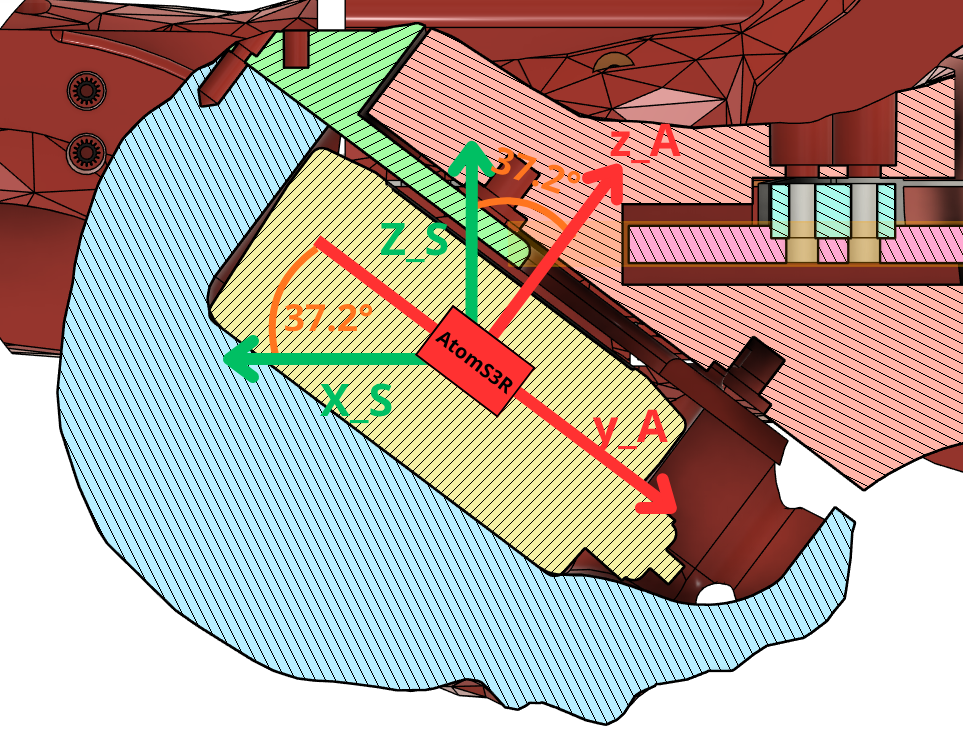
\includegraphics[width=0.6\linewidth]{schemas/AtomS3R_SWUMANOID_orientation_side_view_zoomed.png}
    \caption{Detailed view of the AtomS3R's mechanical tilt in the robot's head.}
    \label{fig:robot_tilt}
\end{figure}

To express the attitude in the robot's Z-Up frame $\mathcal R$, we apply a constant rigid transformation $q_{\text{calib}}$ corresponding to the following sequence of \emph{intrinsic} rotations, about the successive local axes, it demonstrated in the figure~\ref{fig:rotation_repere_schema} :
\begin{enumerate}
  \item $R_1$: a $+37{.}2^\circ$ rotation about the board's \emph{initial} $X$ axis, which compensates the mechanical tilt and straightens the vertical axis \emph{upward}.
  \item $R_2$: a $-90^\circ$ rotation about the \emph{new} $Z'$ axis, which aligns the board axes with the robot's front.
\end{enumerate}

\begin{figure}[H]
    \centering
    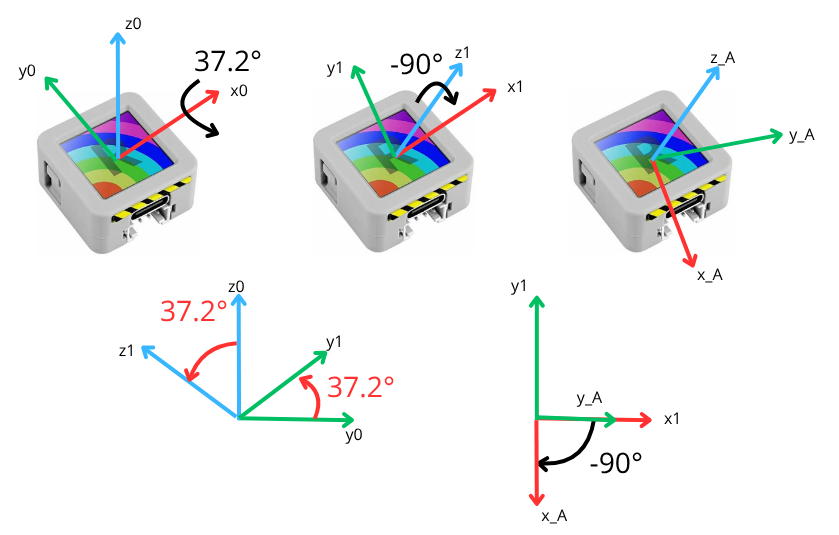
\includegraphics[width=0.9\linewidth]{schemas/AtomS3r_Changement_Repere_Transformation.png}
    \caption{Diagram of the successive rotations applied to the board frame.}
    \label{fig:rotation_repere_schema}
\end{figure}

With the elementary rotation matrices :
\begin{equation}
R_x(\alpha)=\begin{pmatrix}1&0&0\\0&\cos\alpha&-\sin\alpha\\0&\sin\alpha&\cos\alpha\end{pmatrix},
\qquad
R_z(\beta)=\begin{pmatrix}\cos\beta&-\sin\beta&0\\\sin\beta&\cos\beta&0\\0&0&1\end{pmatrix}
\end{equation}
the \emph{intrinsic} composition $R_1$ then $R_2$ about the already-turned axis is obtained by post-multiplication:
\begin{equation}
\mathbf{R}_{\text{calib}}=R_x(37{.}2^\circ)\,R_z(-90^\circ),
\qquad
R_z(-90^\circ)=\begin{pmatrix}0&1&0\\-1&0&0\\0&0&1\end{pmatrix}
\label{eq:Rcalib}
\end{equation}

But the code does not use $\mathbf{R}_{\text{calib}}$ but its equivalent quaternion, to eliminate any singularity. With the axis angle parametrization $q_{\mathbf{n}}(\gamma)=\big(\cos\tfrac{\gamma}{2},\,\mathbf{n}\sin\tfrac{\gamma}{2}\big)$,
\begin{equation}
q_x=q_{\mathbf{e}_x}(37{.}2^\circ)=\big(\cos 18{.}6^\circ,\,\sin 18{.}6^\circ,\,0,\,0\big),
\qquad
q_z=q_{\mathbf{e}_z}(-90^\circ)=\Big(\tfrac{\sqrt{2}}{2},\,0,\,0,\,-\tfrac{\sqrt{2}}{2}\Big)
\end{equation}
\begin{equation}
\boxed{\,q_{\text{calib}}=q_x\otimes q_z\,}
\label{eq:qcalib}
\end{equation}
The robot's absolute attitude, the mount being fixed to the body, results from the post-multiplication
\begin{equation}
\boxed{\,q_{\text{robot}}=q_{\text{raw}}\otimes q_{\text{calib}}\,}
\label{eq:qrobot}
\end{equation}

In goal to let the user sets the current pose as the origin $(0,0,0)$, we store the inverse (conjugate) of the transformed attitude at the trigger instant, $q_{\text{robot}}^{(0)}$:
\begin{equation}
q_{\text{tare}}=\big(q_{\text{robot}}^{(0)}\big)^{-1}=\big(q_{\text{robot}}^{(0)}\big)^{*}
\label{eq:qtare}
\end{equation}
then the displayed attitude is referenced at each sample by
\begin{equation}
\boxed{\,q_{\text{display}}=q_{\text{tare}}\otimes q_{\text{robot}}\,}
\label{eq:qdisplay}
\end{equation}
By construction, $q_{\text{display}}=\mathbf{1}$ (identity, i.e. $0^\circ$) when $q_{\text{robot}}=q_{\text{robot}}^{(0)}$, since $q_{\text{tare}}\otimes q_{\text{robot}}^{(0)}=\big(q_{\text{robot}}^{(0)}\big)^{-1}\otimes q_{\text{robot}}^{(0)}=\mathbf{1}$, any return to the reference pose brings the display rigorously back to zero. This mechanism is also initialized automatically at the first valid sample, which guarantees a zero display at startup, regardless of the board's hardware orientation.

\subsection{Euler Angle Extraction and Low-Pass Filtering}
\label{subsec:extract_filter}

The final angles are extracted from $q_{\text{display}}$ by conversion to Tait--Bryan angles in the order $Z\!-\!Y\!-\!X$. This choice is justified by the structure of the problem, in fact, in a three-axis decomposition, only the \emph{intermediate} axis carries the singularity at $\pm90^\circ$. By placing the \emph{pitch} ($Y$) in the intermediate position, we guarantee that the \emph{roll} ($X$) and the \emph{yaw} ($Z$), the outer axes, stay readable without degeneracy as long as the pitch remains far from $\pm90^\circ$, which is the case for a robot swimming flat. Writing $q_{\text{display}}=(q_w,q_x,q_y,q_z)$, the elements of the associated rotation matrix give :
\begin{empheq}[box=\fbox]{align}
\phi\ (\text{roll}) &= \operatorname{arctan2}\!\big(2(q_yq_z+q_wq_x),\;1-2(q_x^{2}+q_y^{2})\big) \label{eq:roll}\\
\theta\ (\text{pitch}) &= \arcsin\!\big(2(q_wq_y-q_xq_z)\big) \label{eq:pitch}\\
\psi\ (\text{yaw}) &= \operatorname{arctan2}\!\big(2(q_xq_y+q_wq_z),\;1-2(q_y^{2}+q_z^{2})\big) \label{eq:yaw}
\end{empheq}
Only roll~\eqref{eq:roll} and yaw~\eqref{eq:yaw} are kept for display, the yaw follows the right-hand rule about the upward vertical, it means that a positive physical heading produces a positive $\psi$, in agreement with the 3D avatar which is driven directly by $q_{\text{display}}$. The displayed values are $\phi^{\circ}=\tfrac{180}{\pi}\phi$ and $\psi^{\circ}=\tfrac{180}{\pi}\psi$.

\paragraph{Low-pass filter :} Despite the fusion, the angles $\phi^{\circ}$ and $\psi^{\circ}$ keep a residual noise, the IMU measurement noise, motor-induced vibrations, and micro-oscillations at rest. A first-order low-pass filter with exponential moving average is applied \emph{only} to these two final angles. In the continuous regime, away from an angular discontinuity, the discrete recurrence is
\begin{equation}
\boxed{\,y[n]=\alpha\,x[n]+(1-\alpha)\,y[n-1]\,},\qquad \alpha=0{.}2
\label{eq:ema}
\end{equation}
where $x[n]$ is the raw extracted angle~\eqref{eq:roll} or~\eqref{eq:yaw} and $y[n]$ the smoothed displayed value. To avoid any artifact when crossing the $\pm180^\circ$ discontinuity, the implementation works on the \emph{shortest arc} and the difference $x[n]-y[n-1]$ is brought back into $(-180^\circ,180^\circ]$ before weighting :
\begin{equation}
\Delta[n]=\big((x[n]-y[n-1]+180^\circ)\bmod 360^\circ\big)-180^\circ,
\qquad
y[n]=y[n-1]+\alpha\,\Delta[n]
\label{eq:ema_wrap}
\end{equation}
the output itself being folded back into $(-180^\circ,180^\circ]$, away from the discontinuity, \eqref{eq:ema_wrap} is strictly equivalent to~\eqref{eq:ema}. The associated cutoff frequency ($-3$~dB) depends on the sampling period $T_s$, the stream is sent at a variable rate and satisfies exactly :
\begin{equation}
\cos\!\big(2\pi f_c T_s\big)=1-\frac{\alpha^{2}}{2(1-\alpha)},
\qquad\text{so, for }\alpha\ll1,\quad
f_c\approx\frac{\alpha}{2\pi\sqrt{1-\alpha}\;T_s}\approx\frac{0{.}0356}{T_s}
\end{equation}
For a typical rate $f_s=1/T_s\approx50~\mathrm{Hz}$, we get $f_c\approx1{.}8~\mathrm{Hz}$, which effectively attenuates the mechanical vibrations while preserving the dynamics of the swimming stroke. Finally, the 3D avatar model is driven directly by the quaternion $q_{\text{display}}$ demonstrated in the equation \eqref{eq:qdisplay}, unfiltered and free of gimbal lock, while only the numerical display, HUD, receives the smoothed and rounded values $\operatorname{round}(y[n])$.
% \section{Adapting a marine simulation}

\section{Conclusion}
End of the internship!

% ==========================================
%             BIBLIOGRAPHY
% ==========================================
\clearpage

% Hide the default "References" title generated by LaTeX
\renewcommand{\refname}{\vspace{-4ex}}

\section*{Bibliography}
\addcontentsline{toc}{section}{Bibliography}

\begin{spacing}{1.1}
\begin{thebibliography}{99}
\setlength{\itemsep}{0pt}

\vspace{-0.5cm}

\bibitem{nakashima2007swum} M. NAKASHIMA, K. SATOU and Y. MIURA, "Development of Swimming Human Simulation Model Considering Rigid Body Dynamics and Unsteady Fluid Force for Whole Body," Journal of Fluid Science and Technology, vol. 2, no. 1, pp. 56--67, 2007.

\bibitem{nakashima2012optimizing} M. NAKASHIMA, S. MAEDA, T. MIWA and H. ICHIKAWA, "Optimizing Simulation of the Arm Stroke in Crawl Swimming Considering Muscle Strength Characteristics of Athlete Swimmers," Journal of Biomechanical Science and Engineering, vol. 7, no. 2, pp. 102--117, 2012.

\bibitem{swumsuit2005} SWUM DEVELOPER TEAM, "Swumsuit Manual for version 2.2.0," 2005.

\bibitem{chung2013free} C. CHUNG and M. NAKASHIMA, "Free Swimming of the Swimming Humanoid Robot for the Crawl Stroke," Journal of Aero Aqua Bio-mechanisms, vol. 3, no. 1, pp. 118--126, 2013.

\bibitem{chung2014swimming} C. CHUNG and M. NAKASHIMA, "Swimming Humanoid Robot “SWUMANOID” as an Experimental Platform for Research of Human Swimming," Journal of Robotics and Mechatronics, vol. 26, no. 2, pp. 265--266, 2014.

\bibitem{nakashima2016realization} M. NAKASHIMA and K. KUWAHARA, "Realization and swimming performance of the breaststroke by a swimming humanoid robot," ROBOMECH Journal, vol. 3, no. 10, 2016.

\bibitem{sp3485} MAXLINEAR (SIPEX), "SP3485: 3.3V Low Power Half-Duplex RS-485 Transceiver with 10Mbps Data Rate" Datasheet Rev. 2.0.2, August 2021. Accessed on July 7, 2026. URL: \url{https://www.maxlinear.com/product/interface/serial-transceivers/rs-485-rs-422/sp3485}.

\bibitem{max3485} ANALOG DEVICES (MAXIM INTEGRATED), "MAX3483--MAX3491: 3.3V, 10~Mbps RS-485/RS-422 Transceivers," Datasheet, 2014. Accessed on July 10, 2026. URL: \url{https://www.analog.com/en/products/max3485.html}.

\bibitem{esp32s3_uart} ESPRESSIF SYSTEMS, "ESP32-S3 Technical Reference Manual (Version 1.8)," 2024, sec. 26.4.6 (RS485 / Driver Control), pp. 931--932. Accessed on July 13, 2026. URL: \url{https://www.espressif.com/sites/default/files/documentation/esp32-s3_technical_reference_manual_en.pdf}.

\bibitem{mp2307} MONOLITHIC POWER SYSTEMS (MPS), "MP2307: 3A, 23V, 340kHz Synchronous Rectified Step-Down Converter," Datasheet, 2020. Accessed on July 13, 2026. URL: \url{https://www.monolithicpower.com/en/mp2307.html}.

\bibitem{minmax_m78ar05} MINMAX TECHNOLOGY CO., LTD., "M78AR-1 Series: 1A Switching Regulator (7805 Pin-Compatible)," Datasheet, 2018. Accessed on July 14, 2026. URL: \url{https://www.minmaxpower.com/en/product/M78AR-1}.

\bibitem{numerical_recipes} W. H. PRESS, S. A. TEUKOLSKY, W. T. VETTERLING and B. P. FLANNERY, "Numerical Recipes: The Art of Scientific Computing" 3rd ed., Cambridge University Press, 2007, sec. 2.7.1--2.7.2 (Sherman-Morrison and Cyclic Tridiagonal Systems), pp. 77--79.

\bibitem{burden_faires} R. L. BURDEN and J. D. FAIRES, "Numerical Analysis" 9th ed., Brooks/Cole, Cengage Learning, 2010, sec. 6.6 (Special Types of Matrices), pp. 398--409.

\bibitem{madgwick2010} S. O. MADGWICK, A. J. HARRISON and R. VAIDYANATHAN, "Estimation of IMU and MARG orientation using a gradient descent algorithm," IEEE International Conference on Rehabilitation Robotics (ICORR), 2011, pp. 1--7.

\bibitem{mahony2008} R. MAHONY, T. HAMEL and J.-M. PFLIMLIN, "Nonlinear Complementary Filters on the Special Orthogonal Group," IEEE Transactions on Automatic Control, vol. 53, no. 5, pp. 1203--1218, 2008.

\end{thebibliography}
\end{spacing}

\vspace{-0.5cm}

\section*{Sitography}
\addcontentsline{toc}{section}{Sitography}

\begin{thebibliography}{99}
\setcounter{enumiv}{15} % Resume numbering at [11]

\vspace{-0.5cm}

\bibitem{isct2024merger} INSTITUTE OF SCIENCE TOKYO. "Establishment of Institute of Science Tokyo: Merging Tokyo Tech and TMDU." Accessed on June 5, 2026. URL: University official website.

\bibitem{nakashimalab_website} M. NAKASHIMA. "Motomu Nakashima Laboratory - Research Projects." Accessed on June 8, 2026. URL: \url{https://www.hei.sc.e.titech.ac.jp/nakashima_labo/motomu/index2.html}.

\bibitem{m5stack_atoms3} M5STACK TECHNOLOGY CO., LTD. "ATOM S3 Official Documentation." Accessed on June 8, 2026. URL: \url{https://docs.m5stack.com/en/core/AtomS3}.

\bibitem{m5stack_atoms3r} M5STACK TECHNOLOGY CO., LTD. "ATOM S3R Official Documentation." Accessed on June 8, 2026. URL: \url{https://docs.m5stack.com/en/core/AtomS3R}.

\bibitem{dynamixel_x_manual} ROBOTIS CO., LTD. "Dynamixel X-Series Control Table and Protocol 2.0 (e-Manual)." Accessed on June 19, 2026. URL: \url{https://emanual.robotis.com/docs/en/dxl/x/}.

\bibitem{whatwg_sse} WHATWG. "HTML Living Standard --- Server-Sent Events." Accessed on June 12, 2026. URL: \url{https://html.spec.whatwg.org/multipage/server-sent-events.html}.

\bibitem{chartjs} CHART.JS CONTRIBUTORS. "Chart.js --- Open source HTML5 charting library." Accessed on June 12, 2026. URL: \url{https://www.chartjs.org/docs/latest/}.

\bibitem{threejs} THREE.JS AUTHORS. "Three.js --- JavaScript 3D library." Accessed on July 2, 2026. URL: \url{https://threejs.org/docs/}.

\bibitem{m5stack_atomic485} M5STACK TECHNOLOGY CO., LTD. "ATOMIC RS485 Base --- Documentation." Accessed on July 7, 2026. URL: \url{https://docs.m5stack.com/en/atom/atomic485}.

\bibitem{dynamixel_xw430t200} ROBOTIS CO., LTD. "DYNAMIXEL XW430-T200-R (e-Manual)." Accessed on July 21, 2026. URL: \url{https://emanual.robotis.com/docs/en/dxl/x/xw430-t200/}.

\bibitem{dynamixel_xw540t140} ROBOTIS CO., LTD. "DYNAMIXEL XW540-T140-R (e-Manual)." Accessed on July 21, 2026. URL: \url{https://emanual.robotis.com/docs/en/dxl/x/xw540-t140/}.

\bibitem{dynamixel_xw540t260} ROBOTIS CO., LTD. "DYNAMIXEL XW540-T260-R (e-Manual)." Accessed on July 21, 2026. URL: \url{https://emanual.robotis.com/docs/en/dxl/x/xw540-t260/}.

\bibitem{dynamixel_xm540w150} ROBOTIS CO., LTD. "DYNAMIXEL XM540-W150-R (e-Manual)." Accessed on July 21, 2026. URL: \url{https://emanual.robotis.com/docs/en/dxl/x/xm540-w150/}.

\end{thebibliography}

% This line forces the bibliography to appear in the table of contents
%\addcontentsline{toc}{section}{References}
%\bibliographystyle{unsrt} % Display style (unsrt sorts by order of appearance in the text)
% \bibliography{biblio}     % Call the biblio.bib file

\end{document}
